\documentclass[twoside]{book}

% Packages required by doxygen
\usepackage{fixltx2e}
\usepackage{calc}
\usepackage{doxygen}
\usepackage[export]{adjustbox} % also loads graphicx
\usepackage{graphicx}
\usepackage[utf8]{inputenc}
\usepackage{makeidx}
\usepackage{multicol}
\usepackage{multirow}
\PassOptionsToPackage{warn}{textcomp}
\usepackage{textcomp}
\usepackage[nointegrals]{wasysym}
\usepackage[table]{xcolor}

% Font selection
\usepackage[T1]{fontenc}
\usepackage[scaled=.90]{helvet}
\usepackage{courier}
\usepackage{amssymb}
\usepackage{sectsty}
\renewcommand{\familydefault}{\sfdefault}
\allsectionsfont{%
  \fontseries{bc}\selectfont%
  \color{darkgray}%
}
\renewcommand{\DoxyLabelFont}{%
  \fontseries{bc}\selectfont%
  \color{darkgray}%
}
\newcommand{\+}{\discretionary{\mbox{\scriptsize$\hookleftarrow$}}{}{}}

% Page & text layout
\usepackage{geometry}
\geometry{%
  a4paper,%
  top=2.5cm,%
  bottom=2.5cm,%
  left=2.5cm,%
  right=2.5cm%
}
\tolerance=750
\hfuzz=15pt
\hbadness=750
\setlength{\emergencystretch}{15pt}
\setlength{\parindent}{0cm}
\setlength{\parskip}{3ex plus 2ex minus 2ex}
\makeatletter
\renewcommand{\paragraph}{%
  \@startsection{paragraph}{4}{0ex}{-1.0ex}{1.0ex}{%
    \normalfont\normalsize\bfseries\SS@parafont%
  }%
}
\renewcommand{\subparagraph}{%
  \@startsection{subparagraph}{5}{0ex}{-1.0ex}{1.0ex}{%
    \normalfont\normalsize\bfseries\SS@subparafont%
  }%
}
\makeatother

% Headers & footers
\usepackage{fancyhdr}
\pagestyle{fancyplain}
\fancyhead[LE]{\fancyplain{}{\bfseries\thepage}}
\fancyhead[CE]{\fancyplain{}{}}
\fancyhead[RE]{\fancyplain{}{\bfseries\leftmark}}
\fancyhead[LO]{\fancyplain{}{\bfseries\rightmark}}
\fancyhead[CO]{\fancyplain{}{}}
\fancyhead[RO]{\fancyplain{}{\bfseries\thepage}}
\fancyfoot[LE]{\fancyplain{}{}}
\fancyfoot[CE]{\fancyplain{}{}}
\fancyfoot[RE]{\fancyplain{}{\bfseries\scriptsize Generated by Doxygen }}
\fancyfoot[LO]{\fancyplain{}{\bfseries\scriptsize Generated by Doxygen }}
\fancyfoot[CO]{\fancyplain{}{}}
\fancyfoot[RO]{\fancyplain{}{}}
\renewcommand{\footrulewidth}{0.4pt}
\renewcommand{\chaptermark}[1]{%
  \markboth{#1}{}%
}
\renewcommand{\sectionmark}[1]{%
  \markright{\thesection\ #1}%
}

% Indices & bibliography
\usepackage{natbib}
\usepackage[titles]{tocloft}
\setcounter{tocdepth}{3}
\setcounter{secnumdepth}{5}
\makeindex

% Hyperlinks (required, but should be loaded last)
\usepackage{ifpdf}
\ifpdf
  \usepackage[pdftex,pagebackref=true]{hyperref}
\else
  \usepackage[ps2pdf,pagebackref=true]{hyperref}
\fi
\hypersetup{%
  colorlinks=true,%
  linkcolor=blue,%
  citecolor=blue,%
  unicode%
}

% Custom commands
\newcommand{\clearemptydoublepage}{%
  \newpage{\pagestyle{empty}\cleardoublepage}%
}

\usepackage{caption}
\captionsetup{labelsep=space,justification=centering,font={bf},singlelinecheck=off,skip=4pt,position=top}

%===== C O N T E N T S =====

\begin{document}

% Titlepage & ToC
\hypersetup{pageanchor=false,
             bookmarksnumbered=true,
             pdfencoding=unicode
            }
\pagenumbering{alph}
\begin{titlepage}
\vspace*{7cm}
\begin{center}%
{\Large Uniform Data Operator \\[1ex]\large 1.\+0.\+0 alpha 5 }\\
\vspace*{1cm}
{\large Generated by Doxygen 1.8.14}\\
\end{center}
\end{titlepage}
\clearemptydoublepage
\pagenumbering{roman}
\tableofcontents
\clearemptydoublepage
\pagenumbering{arabic}
\hypersetup{pageanchor=true}

%--- Begin generated contents ---
\chapter{Uniform Data Operator}
\label{md__d_1__work__git_hub_uniform-data-operator__r_e_a_d_m_e}
\Hypertarget{md__d_1__work__git_hub_uniform-data-operator__r_e_a_d_m_e}
It\textquotesingle{}s a framework that allow to oparate and manage yours data by unified way, not depending from your data base or prefered format. Standardize your data structures and avoid adjust of your product only for one storage type that could be not suitable for you in future.

\section*{Modules}

\subsection*{Binnary Handler}

Provides base A\+PI for binary serizliation process.

\subsection*{S\+Q\+L\+Operator\+Handler}

Provides methods that simplify converting of app\textquotesingle{}s data to query format. Inform subscribers about {\ttfamily I\+Sql\+Pperators} events. Provides access to current {\ttfamily Active} S\+QL operator.

\subsection*{Attributes\+Handler}

Provides A\+PI thats simplify working with U\+DO attributes and members data.

\subsection*{Included operators\+:}


\begin{DoxyItemize}
\item {\ttfamily My\+S\+Q\+L\+Data\+Operator} -\/ provides uniform way to manage your data via My\+S\+QL database.
\end{DoxyItemize}

\section*{F.\+A.\+Q.}

\subsection*{How to describe table class/struct?}

\subsubsection*{Conception}

At first you need to understand conception of work with data and them representations at database.

For every table on server that must be compatible with your application on native level you need to provide the class/structure with compatible and correct described fields/properties.

This class/structure would be a bridge betwee your local data and server representation.

\subsubsection*{Describing}

Describing of data making by using of attributs from {\ttfamily \mbox{\hyperlink{namespace_uniform_data_operator_1_1_sql_1_1_tables_1_1_attributes}{Uniform\+Data\+Operator.\+Sql.\+Tables.\+Attributes}}} namespace. (Custom attributes and modifiers can has other namespace).


\begin{DoxyEnumerate}
\item Define {\ttfamily Table} attribute for your class/structure. Describe correct scheme and table name.
\item Define {\ttfamily System.\+Serializable} attribute for your class.
\item For every field/property that would be a column defind {\ttfamily Column} attribute. Set column name and type at constructor.
\item Define additive columns\textquotesingle{} attributes like {\ttfamily is\+Primary\+Key}, {\ttfamily is\+Auto\+Increment}, {\ttfamily Commentary}, etc. More details you can wind in source or offline documetation.
\end{DoxyEnumerate}

\subsection*{How operator defines what would be included in auto generated read/write queries?}

Every operator can has a different algorithm related to specific requirements of database server. But a common idea is mapping of you \textquotesingle{}Table\textquotesingle{} defined class by {\ttfamily Column} attributes and generate the queries based on them settings and values.

If some attribute affecting algorithm then that described at that\textquotesingle{}s summary.

\subsection*{I need to manage data received from server. How I can do it?}

Just use a property as column. Then you would be able to manage a complex get/set algorithms during operator actions.

\subsection*{Can I add supporting of other S\+QL server?}

Sure. Just create you Server\+Name\+Operator that implement I\+Sql\+Operator interface and your data described by U\+DO\textquotesingle{}s attributes would be compatible with your specific server.

Use the default My\+Sql\+Data\+Operator (group of partial classes) as example. Them are pretty good documented. If you done this job please consider sharing this source as contribution into U\+DO.

\subsection*{My S\+QL server incompatible with Db\+Data\+Type\textquotesingle{}s indexes. How I can adjust my data?}

By default {\ttfamily Column} attribute described via {\ttfamily Db\+Data\+Type} that mostly unusable for huge count of types that custom for every different S\+QL server. If you faced with such kind of problem so just create your own modifying attribute that would be used on your custom {\ttfamily I\+Sql\+Operator} instance.

Use {\ttfamily \mbox{\hyperlink{class_uniform_data_operator_1_1_sql_1_1_my_sql_1_1_attributes_1_1_my_sql_d_b_type_override}{Uniform\+Data\+Operator.\+Sql.\+My\+Sql.\+Attributes.\+My\+Sql\+D\+B\+Type\+Override}}} as example for your source. Check how it using at {\ttfamily My\+Sql\+Data\+Operator\+Commands.\+cs} in {\ttfamily Column\+Declaration\+Command} method.

\subsection*{Auto write/read not enough flexible for me. How I can make custom query?}

Auto managing of duplex exchanging of data with S\+QL server it\textquotesingle{}s just a high end feature. But not the only way to manage your uniformed data.

All what you need it\textquotesingle{}s pipe down on one level and start direct work with your {\ttfamily I\+Sql\+Operator} instance.

Make your own S\+QL query suitable by your specific task and send it to server via {\ttfamily Sql\+Operato\+Handler.\+Active} by use one of provided methods \+:
\begin{DoxyItemize}
\item {\ttfamily Execute\+Non\+Query}
\item {\ttfamily Execute\+Scalar}
\item {\ttfamily Execute\+Reader}
\item {\ttfamily Count}
\end{DoxyItemize}

\subsection*{How to establish connection with server?}


\begin{DoxyEnumerate}
\item Create and instance of your {\ttfamily I\+Sql\+Operator} instance.
\item Initialize properties of your {\ttfamily I\+Sql\+Operator} instance\+:
\begin{DoxyItemize}
\item {\ttfamily string Server}
\item {\ttfamily int Port}
\item {\ttfamily string Database}
\item {\ttfamily string User\+Id}
\item {\ttfamily string Password}
\end{DoxyItemize}
\item Call {\ttfamily Initialize} method on your {\ttfamily I\+Sql\+Operator} instance.
\item Call {\ttfamily Open\+Connection} method on your {\ttfamily I\+Sql\+Operator} instance.
\item Execute your S\+QL query.
\item Call {\ttfamily Close\+Connection} method on your {\ttfamily I\+Sql\+Operator} instance. 
\end{DoxyEnumerate}
\chapter{Namespace Index}
\section{Packages}
Here are the packages with brief descriptions (if available)\+:\begin{DoxyCompactList}
\item\contentsline{section}{\mbox{\hyperlink{namespace_base_tests}{Base\+Tests}} }{\pageref{namespace_base_tests}}{}
\item\contentsline{section}{\mbox{\hyperlink{namespace_base_tests_1_1_binary}{Base\+Tests.\+Binary}} }{\pageref{namespace_base_tests_1_1_binary}}{}
\item\contentsline{section}{\mbox{\hyperlink{namespace_base_tests_1_1_types}{Base\+Tests.\+Types}} }{\pageref{namespace_base_tests_1_1_types}}{}
\item\contentsline{section}{\mbox{\hyperlink{namespace_my_s_q_l_tests}{My\+S\+Q\+L\+Tests}} }{\pageref{namespace_my_s_q_l_tests}}{}
\item\contentsline{section}{\mbox{\hyperlink{namespace_uniform_data_operator}{Uniform\+Data\+Operator}} }{\pageref{namespace_uniform_data_operator}}{}
\item\contentsline{section}{\mbox{\hyperlink{namespace_uniform_data_operator_1_1_binary}{Uniform\+Data\+Operator.\+Binary}} }{\pageref{namespace_uniform_data_operator_1_1_binary}}{}
\item\contentsline{section}{\mbox{\hyperlink{namespace_uniform_data_operator_1_1_sql}{Uniform\+Data\+Operator.\+Sql}} }{\pageref{namespace_uniform_data_operator_1_1_sql}}{}
\item\contentsline{section}{\mbox{\hyperlink{namespace_uniform_data_operator_1_1_sql_1_1_attributes}{Uniform\+Data\+Operator.\+Sql.\+Attributes}} }{\pageref{namespace_uniform_data_operator_1_1_sql_1_1_attributes}}{}
\item\contentsline{section}{\mbox{\hyperlink{namespace_uniform_data_operator_1_1_sql_1_1_attributes_1_1_modifiers}{Uniform\+Data\+Operator.\+Sql.\+Attributes.\+Modifiers}} }{\pageref{namespace_uniform_data_operator_1_1_sql_1_1_attributes_1_1_modifiers}}{}
\item\contentsline{section}{\mbox{\hyperlink{namespace_uniform_data_operator_1_1_sql_1_1_my_sql}{Uniform\+Data\+Operator.\+Sql.\+My\+Sql}} }{\pageref{namespace_uniform_data_operator_1_1_sql_1_1_my_sql}}{}
\item\contentsline{section}{\mbox{\hyperlink{namespace_uniform_data_operator_1_1_sql_1_1_my_sql_1_1_attributes}{Uniform\+Data\+Operator.\+Sql.\+My\+Sql.\+Attributes}} }{\pageref{namespace_uniform_data_operator_1_1_sql_1_1_my_sql_1_1_attributes}}{}
\end{DoxyCompactList}

\chapter{Hierarchical Index}
\section{Class Hierarchy}
This inheritance list is sorted roughly, but not completely, alphabetically\+:\begin{DoxyCompactList}
\item Attribute\begin{DoxyCompactList}
\item \contentsline{section}{Uniform\+Data\+Operator.\+Sql.\+My\+Sql.\+Attributes.\+My\+Sql\+D\+B\+Type\+Override}{\pageref{class_uniform_data_operator_1_1_sql_1_1_my_sql_1_1_attributes_1_1_my_sql_d_b_type_override}}{}
\item \contentsline{section}{Uniform\+Data\+Operator.\+Sql.\+Tables.\+Attributes.\+Column}{\pageref{class_uniform_data_operator_1_1_sql_1_1_tables_1_1_attributes_1_1_column}}{}
\item \contentsline{section}{Uniform\+Data\+Operator.\+Sql.\+Tables.\+Attributes.\+Commentary}{\pageref{class_uniform_data_operator_1_1_sql_1_1_tables_1_1_attributes_1_1_commentary}}{}
\item \contentsline{section}{Uniform\+Data\+Operator.\+Sql.\+Tables.\+Attributes.\+Default}{\pageref{class_uniform_data_operator_1_1_sql_1_1_tables_1_1_attributes_1_1_default}}{}
\begin{DoxyCompactList}
\item \contentsline{section}{Uniform\+Data\+Operator.\+Sql.\+Tables.\+Attributes.\+Is\+Generated}{\pageref{class_uniform_data_operator_1_1_sql_1_1_tables_1_1_attributes_1_1_is_generated}}{}
\end{DoxyCompactList}
\item \contentsline{section}{Uniform\+Data\+Operator.\+Sql.\+Tables.\+Attributes.\+Is\+Auto\+Increment}{\pageref{class_uniform_data_operator_1_1_sql_1_1_tables_1_1_attributes_1_1_is_auto_increment}}{}
\item \contentsline{section}{Uniform\+Data\+Operator.\+Sql.\+Tables.\+Attributes.\+Is\+Binary}{\pageref{class_uniform_data_operator_1_1_sql_1_1_tables_1_1_attributes_1_1_is_binary}}{}
\item \contentsline{section}{Uniform\+Data\+Operator.\+Sql.\+Tables.\+Attributes.\+Is\+Foreign\+Key}{\pageref{class_uniform_data_operator_1_1_sql_1_1_tables_1_1_attributes_1_1_is_foreign_key}}{}
\item \contentsline{section}{Uniform\+Data\+Operator.\+Sql.\+Tables.\+Attributes.\+Is\+Not\+Null}{\pageref{class_uniform_data_operator_1_1_sql_1_1_tables_1_1_attributes_1_1_is_not_null}}{}
\item \contentsline{section}{Uniform\+Data\+Operator.\+Sql.\+Tables.\+Attributes.\+Is\+Primary\+Key}{\pageref{class_uniform_data_operator_1_1_sql_1_1_tables_1_1_attributes_1_1_is_primary_key}}{}
\item \contentsline{section}{Uniform\+Data\+Operator.\+Sql.\+Tables.\+Attributes.\+Is\+Unique}{\pageref{class_uniform_data_operator_1_1_sql_1_1_tables_1_1_attributes_1_1_is_unique}}{}
\item \contentsline{section}{Uniform\+Data\+Operator.\+Sql.\+Tables.\+Attributes.\+Is\+Unsigned}{\pageref{class_uniform_data_operator_1_1_sql_1_1_tables_1_1_attributes_1_1_is_unsigned}}{}
\item \contentsline{section}{Uniform\+Data\+Operator.\+Sql.\+Tables.\+Attributes.\+Is\+Zero\+Fill}{\pageref{class_uniform_data_operator_1_1_sql_1_1_tables_1_1_attributes_1_1_is_zero_fill}}{}
\item \contentsline{section}{Uniform\+Data\+Operator.\+Sql.\+Tables.\+Attributes.\+Modifiers.\+Set\+Query\+Ignore}{\pageref{class_uniform_data_operator_1_1_sql_1_1_tables_1_1_attributes_1_1_modifiers_1_1_set_query_ignore}}{}
\item \contentsline{section}{Uniform\+Data\+Operator.\+Sql.\+Tables.\+Attributes.\+Table}{\pageref{class_uniform_data_operator_1_1_sql_1_1_tables_1_1_attributes_1_1_table}}{}
\end{DoxyCompactList}
\item \contentsline{section}{Uniform\+Data\+Operator.\+Attributes\+Handler}{\pageref{class_uniform_data_operator_1_1_attributes_handler}}{}
\item \contentsline{section}{Uniform\+Data\+Operator.\+Binary.\+Binary\+Handler}{\pageref{class_uniform_data_operator_1_1_binary_1_1_binary_handler}}{}
\item \contentsline{section}{Base\+Tests.\+Binary.\+Binary\+Handler\+Tests}{\pageref{class_base_tests_1_1_binary_1_1_binary_handler_tests}}{}
\item \contentsline{section}{Base\+Tests.\+Types.\+Blob\+Type}{\pageref{class_base_tests_1_1_types_1_1_blob_type}}{}
\item \contentsline{section}{Uniform\+Data\+Operator.\+Sql.\+I\+Sql\+Operator}{\pageref{interface_uniform_data_operator_1_1_sql_1_1_i_sql_operator}}{}
\begin{DoxyCompactList}
\item \contentsline{section}{Uniform\+Data\+Operator.\+Sql.\+My\+Sql.\+My\+Sql\+Data\+Operator}{\pageref{class_uniform_data_operator_1_1_sql_1_1_my_sql_1_1_my_sql_data_operator}}{}
\item \contentsline{section}{Uniform\+Data\+Operator.\+Sql.\+My\+Sql.\+My\+Sql\+Data\+Operator}{\pageref{class_uniform_data_operator_1_1_sql_1_1_my_sql_1_1_my_sql_data_operator}}{}
\item \contentsline{section}{Uniform\+Data\+Operator.\+Sql.\+My\+Sql.\+My\+Sql\+Data\+Operator}{\pageref{class_uniform_data_operator_1_1_sql_1_1_my_sql_1_1_my_sql_data_operator}}{}
\item \contentsline{section}{Uniform\+Data\+Operator.\+Sql.\+My\+Sql.\+My\+Sql\+Data\+Operator}{\pageref{class_uniform_data_operator_1_1_sql_1_1_my_sql_1_1_my_sql_data_operator}}{}
\item \contentsline{section}{Uniform\+Data\+Operator.\+Sql.\+My\+Sql.\+My\+Sql\+Data\+Operator}{\pageref{class_uniform_data_operator_1_1_sql_1_1_my_sql_1_1_my_sql_data_operator}}{}
\item \contentsline{section}{Uniform\+Data\+Operator.\+Sql.\+My\+Sql.\+My\+Sql\+Data\+Operator}{\pageref{class_uniform_data_operator_1_1_sql_1_1_my_sql_1_1_my_sql_data_operator}}{}
\end{DoxyCompactList}
\item \contentsline{section}{My\+S\+Q\+L\+Tests.\+Local}{\pageref{class_my_s_q_l_tests_1_1_local}}{}
\item \contentsline{section}{Uniform\+Data\+Operator.\+Sql.\+Sql\+Operator\+Handler}{\pageref{class_uniform_data_operator_1_1_sql_1_1_sql_operator_handler}}{}
\item \contentsline{section}{Base\+Tests.\+Types.\+Table2\+Type}{\pageref{class_base_tests_1_1_types_1_1_table2_type}}{}
\item \contentsline{section}{Base\+Tests.\+Types.\+Table3\+Type}{\pageref{class_base_tests_1_1_types_1_1_table3_type}}{}
\item \contentsline{section}{Base\+Tests.\+Types.\+Table4\+Type}{\pageref{class_base_tests_1_1_types_1_1_table4_type}}{}
\item \contentsline{section}{Base\+Tests.\+Types.\+Table5\+Type}{\pageref{class_base_tests_1_1_types_1_1_table5_type}}{}
\item \contentsline{section}{My\+S\+Q\+L\+Tests.\+Tables}{\pageref{class_my_s_q_l_tests_1_1_tables}}{}
\item \contentsline{section}{Base\+Tests.\+Types.\+Table\+Type}{\pageref{class_base_tests_1_1_types_1_1_table_type}}{}
\end{DoxyCompactList}

\chapter{Class Index}
\section{Class List}
Here are the classes, structs, unions and interfaces with brief descriptions\+:\begin{DoxyCompactList}
\item\contentsline{section}{\mbox{\hyperlink{class_uniform_data_operator_1_1_attributes_handler}{Uniform\+Data\+Operator.\+Attributes\+Handler}} \\*Provides A\+PI to handle attributes. }{\pageref{class_uniform_data_operator_1_1_attributes_handler}}{}
\item\contentsline{section}{\mbox{\hyperlink{class_uniform_data_operator_1_1_binary_1_1_binary_handler}{Uniform\+Data\+Operator.\+Binary.\+Binary\+Handler}} \\*Provide A\+PI to working with binary files. }{\pageref{class_uniform_data_operator_1_1_binary_1_1_binary_handler}}{}
\item\contentsline{section}{\mbox{\hyperlink{class_base_tests_1_1_binary_1_1_binary_handler_tests}{Base\+Tests.\+Binary.\+Binary\+Handler\+Tests}} }{\pageref{class_base_tests_1_1_binary_1_1_binary_handler_tests}}{}
\item\contentsline{section}{\mbox{\hyperlink{class_base_tests_1_1_types_1_1_blob_type}{Base\+Tests.\+Types.\+Blob\+Type}} }{\pageref{class_base_tests_1_1_types_1_1_blob_type}}{}
\item\contentsline{section}{\mbox{\hyperlink{class_uniform_data_operator_1_1_sql_1_1_tables_1_1_attributes_1_1_column}{Uniform\+Data\+Operator.\+Sql.\+Tables.\+Attributes.\+Column}} }{\pageref{class_uniform_data_operator_1_1_sql_1_1_tables_1_1_attributes_1_1_column}}{}
\item\contentsline{section}{\mbox{\hyperlink{class_uniform_data_operator_1_1_sql_1_1_tables_1_1_attributes_1_1_commentary}{Uniform\+Data\+Operator.\+Sql.\+Tables.\+Attributes.\+Commentary}} \\*Add commentary to S\+QL table. }{\pageref{class_uniform_data_operator_1_1_sql_1_1_tables_1_1_attributes_1_1_commentary}}{}
\item\contentsline{section}{\mbox{\hyperlink{class_uniform_data_operator_1_1_sql_1_1_tables_1_1_attributes_1_1_default}{Uniform\+Data\+Operator.\+Sql.\+Tables.\+Attributes.\+Default}} \\*Add default valu to the field. }{\pageref{class_uniform_data_operator_1_1_sql_1_1_tables_1_1_attributes_1_1_default}}{}
\item\contentsline{section}{\mbox{\hyperlink{class_uniform_data_operator_1_1_sql_1_1_tables_1_1_attributes_1_1_is_auto_increment}{Uniform\+Data\+Operator.\+Sql.\+Tables.\+Attributes.\+Is\+Auto\+Increment}} \\*Is value of this column would incremented relative to previous one during init. }{\pageref{class_uniform_data_operator_1_1_sql_1_1_tables_1_1_attributes_1_1_is_auto_increment}}{}
\item\contentsline{section}{\mbox{\hyperlink{class_uniform_data_operator_1_1_sql_1_1_tables_1_1_attributes_1_1_is_binary}{Uniform\+Data\+Operator.\+Sql.\+Tables.\+Attributes.\+Is\+Binary}} \\*Is data would stored in binary format. }{\pageref{class_uniform_data_operator_1_1_sql_1_1_tables_1_1_attributes_1_1_is_binary}}{}
\item\contentsline{section}{\mbox{\hyperlink{class_uniform_data_operator_1_1_sql_1_1_tables_1_1_attributes_1_1_is_foreign_key}{Uniform\+Data\+Operator.\+Sql.\+Tables.\+Attributes.\+Is\+Foreign\+Key}} \\*Mark fireld as foreign key to other column. }{\pageref{class_uniform_data_operator_1_1_sql_1_1_tables_1_1_attributes_1_1_is_foreign_key}}{}
\item\contentsline{section}{\mbox{\hyperlink{class_uniform_data_operator_1_1_sql_1_1_tables_1_1_attributes_1_1_is_generated}{Uniform\+Data\+Operator.\+Sql.\+Tables.\+Attributes.\+Is\+Generated}} \\*Mark field as generated. }{\pageref{class_uniform_data_operator_1_1_sql_1_1_tables_1_1_attributes_1_1_is_generated}}{}
\item\contentsline{section}{\mbox{\hyperlink{class_uniform_data_operator_1_1_sql_1_1_tables_1_1_attributes_1_1_is_not_null}{Uniform\+Data\+Operator.\+Sql.\+Tables.\+Attributes.\+Is\+Not\+Null}} \\*Is value always not null. }{\pageref{class_uniform_data_operator_1_1_sql_1_1_tables_1_1_attributes_1_1_is_not_null}}{}
\item\contentsline{section}{\mbox{\hyperlink{class_uniform_data_operator_1_1_sql_1_1_tables_1_1_attributes_1_1_is_primary_key}{Uniform\+Data\+Operator.\+Sql.\+Tables.\+Attributes.\+Is\+Primary\+Key}} \\*Is it\textquotesingle{}s primary key. }{\pageref{class_uniform_data_operator_1_1_sql_1_1_tables_1_1_attributes_1_1_is_primary_key}}{}
\item\contentsline{section}{\mbox{\hyperlink{interface_uniform_data_operator_1_1_sql_1_1_i_sql_operator}{Uniform\+Data\+Operator.\+Sql.\+I\+Sql\+Operator}} \\*Implement that interface to provide possiblity to controll your data base by using S\+QL queryes. }{\pageref{interface_uniform_data_operator_1_1_sql_1_1_i_sql_operator}}{}
\item\contentsline{section}{\mbox{\hyperlink{class_uniform_data_operator_1_1_sql_1_1_tables_1_1_attributes_1_1_is_unique}{Uniform\+Data\+Operator.\+Sql.\+Tables.\+Attributes.\+Is\+Unique}} \\*Is this value must be unique by this column. }{\pageref{class_uniform_data_operator_1_1_sql_1_1_tables_1_1_attributes_1_1_is_unique}}{}
\item\contentsline{section}{\mbox{\hyperlink{class_uniform_data_operator_1_1_sql_1_1_tables_1_1_attributes_1_1_is_unsigned}{Uniform\+Data\+Operator.\+Sql.\+Tables.\+Attributes.\+Is\+Unsigned}} \\*Is not have signs after dot. }{\pageref{class_uniform_data_operator_1_1_sql_1_1_tables_1_1_attributes_1_1_is_unsigned}}{}
\item\contentsline{section}{\mbox{\hyperlink{class_uniform_data_operator_1_1_sql_1_1_tables_1_1_attributes_1_1_is_zero_fill}{Uniform\+Data\+Operator.\+Sql.\+Tables.\+Attributes.\+Is\+Zero\+Fill}} \\*Is value wold be willed by zero by default. Only for numerical columns. }{\pageref{class_uniform_data_operator_1_1_sql_1_1_tables_1_1_attributes_1_1_is_zero_fill}}{}
\item\contentsline{section}{\mbox{\hyperlink{class_my_s_q_l_tests_1_1_local}{My\+S\+Q\+L\+Tests.\+Local}} }{\pageref{class_my_s_q_l_tests_1_1_local}}{}
\item\contentsline{section}{\mbox{\hyperlink{class_uniform_data_operator_1_1_sql_1_1_my_sql_1_1_my_sql_data_operator}{Uniform\+Data\+Operator.\+Sql.\+My\+Sql.\+My\+Sql\+Data\+Operator}} \\*Operator that provides possibility to operate data on My\+S\+QL data base server. }{\pageref{class_uniform_data_operator_1_1_sql_1_1_my_sql_1_1_my_sql_data_operator}}{}
\item\contentsline{section}{\mbox{\hyperlink{class_uniform_data_operator_1_1_sql_1_1_my_sql_1_1_attributes_1_1_my_sql_d_b_type_override}{Uniform\+Data\+Operator.\+Sql.\+My\+Sql.\+Attributes.\+My\+Sql\+D\+B\+Type\+Override}} \\*Attribute that can be defined to override standard D\+B\+Type defined in Column attribute, for columns that would created in \mbox{\hyperlink{namespace_uniform_data_operator_1_1_sql_1_1_my_sql}{My\+Sql}} tables. }{\pageref{class_uniform_data_operator_1_1_sql_1_1_my_sql_1_1_attributes_1_1_my_sql_d_b_type_override}}{}
\item\contentsline{section}{\mbox{\hyperlink{class_uniform_data_operator_1_1_sql_1_1_tables_1_1_attributes_1_1_modifiers_1_1_set_query_ignore}{Uniform\+Data\+Operator.\+Sql.\+Tables.\+Attributes.\+Modifiers.\+Set\+Query\+Ignore}} \\*Can be defined to ignore of writing this value during set-\/like queries to server. }{\pageref{class_uniform_data_operator_1_1_sql_1_1_tables_1_1_attributes_1_1_modifiers_1_1_set_query_ignore}}{}
\item\contentsline{section}{\mbox{\hyperlink{class_uniform_data_operator_1_1_sql_1_1_sql_operator_handler}{Uniform\+Data\+Operator.\+Sql.\+Sql\+Operator\+Handler}} \\*Contains base catalog of uniform queries that strongly simplify managing of the data base. }{\pageref{class_uniform_data_operator_1_1_sql_1_1_sql_operator_handler}}{}
\item\contentsline{section}{\mbox{\hyperlink{class_uniform_data_operator_1_1_sql_1_1_tables_1_1_attributes_1_1_table}{Uniform\+Data\+Operator.\+Sql.\+Tables.\+Attributes.\+Table}} \\*Attribute that would force to automatic generation of table on your S\+QL server suitable for declered members in class or structure. }{\pageref{class_uniform_data_operator_1_1_sql_1_1_tables_1_1_attributes_1_1_table}}{}
\item\contentsline{section}{\mbox{\hyperlink{class_base_tests_1_1_types_1_1_table2_type}{Base\+Tests.\+Types.\+Table2\+Type}} }{\pageref{class_base_tests_1_1_types_1_1_table2_type}}{}
\item\contentsline{section}{\mbox{\hyperlink{class_base_tests_1_1_types_1_1_table3_type}{Base\+Tests.\+Types.\+Table3\+Type}} }{\pageref{class_base_tests_1_1_types_1_1_table3_type}}{}
\item\contentsline{section}{\mbox{\hyperlink{class_base_tests_1_1_types_1_1_table4_type}{Base\+Tests.\+Types.\+Table4\+Type}} }{\pageref{class_base_tests_1_1_types_1_1_table4_type}}{}
\item\contentsline{section}{\mbox{\hyperlink{class_base_tests_1_1_types_1_1_table5_type}{Base\+Tests.\+Types.\+Table5\+Type}} }{\pageref{class_base_tests_1_1_types_1_1_table5_type}}{}
\item\contentsline{section}{\mbox{\hyperlink{class_my_s_q_l_tests_1_1_tables}{My\+S\+Q\+L\+Tests.\+Tables}} }{\pageref{class_my_s_q_l_tests_1_1_tables}}{}
\item\contentsline{section}{\mbox{\hyperlink{class_base_tests_1_1_types_1_1_table_type}{Base\+Tests.\+Types.\+Table\+Type}} }{\pageref{class_base_tests_1_1_types_1_1_table_type}}{}
\end{DoxyCompactList}

\chapter{Namespace Documentation}
\hypertarget{namespace_base_tests}{}\section{Base\+Tests Namespace Reference}
\label{namespace_base_tests}\index{Base\+Tests@{Base\+Tests}}
\subsection*{Namespaces}
\begin{DoxyCompactItemize}
\end{DoxyCompactItemize}

\hypertarget{namespace_base_tests_1_1_binary}{}\section{Base\+Tests.\+Binary Namespace Reference}
\label{namespace_base_tests_1_1_binary}\index{Base\+Tests.\+Binary@{Base\+Tests.\+Binary}}
\subsection*{Classes}
\begin{DoxyCompactItemize}
\item 
class \mbox{\hyperlink{class_base_tests_1_1_binary_1_1_binary_handler_tests}{Binary\+Handler\+Tests}}
\end{DoxyCompactItemize}

\hypertarget{namespace_base_tests_1_1_types}{}\section{Base\+Tests.\+Types Namespace Reference}
\label{namespace_base_tests_1_1_types}\index{Base\+Tests.\+Types@{Base\+Tests.\+Types}}
\subsection*{Classes}
\begin{DoxyCompactItemize}
\item 
class \mbox{\hyperlink{class_base_tests_1_1_types_1_1_blob_type}{Blob\+Type}}
\item 
class \mbox{\hyperlink{class_base_tests_1_1_types_1_1_table2_type}{Table2\+Type}}
\item 
class \mbox{\hyperlink{class_base_tests_1_1_types_1_1_table3_type}{Table3\+Type}}
\item 
class \mbox{\hyperlink{class_base_tests_1_1_types_1_1_table4_type}{Table4\+Type}}
\item 
class \mbox{\hyperlink{class_base_tests_1_1_types_1_1_table5_type}{Table5\+Type}}
\item 
class \mbox{\hyperlink{class_base_tests_1_1_types_1_1_table_type}{Table\+Type}}
\end{DoxyCompactItemize}

\hypertarget{namespace_my_s_q_l_tests}{}\section{My\+S\+Q\+L\+Tests Namespace Reference}
\label{namespace_my_s_q_l_tests}\index{My\+S\+Q\+L\+Tests@{My\+S\+Q\+L\+Tests}}
\subsection*{Classes}
\begin{DoxyCompactItemize}
\item 
class \mbox{\hyperlink{class_my_s_q_l_tests_1_1_local}{Local}}
\item 
class \mbox{\hyperlink{class_my_s_q_l_tests_1_1_tables}{Tables}}
\end{DoxyCompactItemize}

\hypertarget{namespace_uniform_data_operator}{}\section{Uniform\+Data\+Operator Namespace Reference}
\label{namespace_uniform_data_operator}\index{Uniform\+Data\+Operator@{Uniform\+Data\+Operator}}
\subsection*{Namespaces}
\begin{DoxyCompactItemize}
\end{DoxyCompactItemize}
\subsection*{Classes}
\begin{DoxyCompactItemize}
\item 
class \mbox{\hyperlink{class_uniform_data_operator_1_1_attributes_handler}{Attributes\+Handler}}
\begin{DoxyCompactList}\small\item\em Provides A\+PI to handle attributes. \end{DoxyCompactList}\end{DoxyCompactItemize}

\hypertarget{namespace_uniform_data_operator_1_1_binary}{}\section{Uniform\+Data\+Operator.\+Binary Namespace Reference}
\label{namespace_uniform_data_operator_1_1_binary}\index{Uniform\+Data\+Operator.\+Binary@{Uniform\+Data\+Operator.\+Binary}}
\subsection*{Classes}
\begin{DoxyCompactItemize}
\item 
class \mbox{\hyperlink{class_uniform_data_operator_1_1_binary_1_1_binary_handler}{Binary\+Handler}}
\begin{DoxyCompactList}\small\item\em Provide A\+PI to working with binary files. \end{DoxyCompactList}\end{DoxyCompactItemize}

\hypertarget{namespace_uniform_data_operator_1_1_sql}{}\section{Uniform\+Data\+Operator.\+Sql Namespace Reference}
\label{namespace_uniform_data_operator_1_1_sql}\index{Uniform\+Data\+Operator.\+Sql@{Uniform\+Data\+Operator.\+Sql}}
\subsection*{Namespaces}
\begin{DoxyCompactItemize}
\end{DoxyCompactItemize}
\subsection*{Classes}
\begin{DoxyCompactItemize}
\item 
interface \mbox{\hyperlink{interface_uniform_data_operator_1_1_sql_1_1_i_sql_operator}{I\+Sql\+Operator}}
\begin{DoxyCompactList}\small\item\em Implement that interface to provide possiblity to controll your database by using S\+QL queryes. \end{DoxyCompactList}\item 
class \mbox{\hyperlink{class_uniform_data_operator_1_1_sql_1_1_sql_operator_handler}{Sql\+Operator\+Handler}}
\begin{DoxyCompactList}\small\item\em Contains base catalog of uniform queries that strongly simplify managing of the database. \end{DoxyCompactList}\end{DoxyCompactItemize}

\hypertarget{namespace_uniform_data_operator_1_1_sql_1_1_attributes}{}\section{Uniform\+Data\+Operator.\+Sql.\+Attributes Namespace Reference}
\label{namespace_uniform_data_operator_1_1_sql_1_1_attributes}\index{Uniform\+Data\+Operator.\+Sql.\+Attributes@{Uniform\+Data\+Operator.\+Sql.\+Attributes}}
\subsection*{Namespaces}
\begin{DoxyCompactItemize}
\end{DoxyCompactItemize}
\subsection*{Classes}
\begin{DoxyCompactItemize}
\item 
class \mbox{\hyperlink{class_uniform_data_operator_1_1_sql_1_1_attributes_1_1_column}{Column}}
\begin{DoxyCompactList}\small\item\em Descriptro of data base table\textquotesingle{}s column. \end{DoxyCompactList}\item 
class \mbox{\hyperlink{class_uniform_data_operator_1_1_sql_1_1_attributes_1_1_commentary}{Commentary}}
\begin{DoxyCompactList}\small\item\em Add commentary to S\+QL table. \end{DoxyCompactList}\item 
class \mbox{\hyperlink{class_uniform_data_operator_1_1_sql_1_1_attributes_1_1_default}{Default}}
\begin{DoxyCompactList}\small\item\em Add default valu to the field. \end{DoxyCompactList}\item 
class \mbox{\hyperlink{class_uniform_data_operator_1_1_sql_1_1_attributes_1_1_is_auto_increment}{Is\+Auto\+Increment}}
\begin{DoxyCompactList}\small\item\em Is value of this column would incremented relative to previous one during init. \end{DoxyCompactList}\item 
class \mbox{\hyperlink{class_uniform_data_operator_1_1_sql_1_1_attributes_1_1_is_binary}{Is\+Binary}}
\begin{DoxyCompactList}\small\item\em Is data would stored in binary format. \end{DoxyCompactList}\item 
class \mbox{\hyperlink{class_uniform_data_operator_1_1_sql_1_1_attributes_1_1_is_foreign_key}{Is\+Foreign\+Key}}
\begin{DoxyCompactList}\small\item\em Mark fireld as foreign key to other column. \end{DoxyCompactList}\item 
class \mbox{\hyperlink{class_uniform_data_operator_1_1_sql_1_1_attributes_1_1_is_generated}{Is\+Generated}}
\begin{DoxyCompactList}\small\item\em Mark field as generated. \end{DoxyCompactList}\item 
class \mbox{\hyperlink{class_uniform_data_operator_1_1_sql_1_1_attributes_1_1_is_not_null}{Is\+Not\+Null}}
\begin{DoxyCompactList}\small\item\em Is value always not null. \end{DoxyCompactList}\item 
class \mbox{\hyperlink{class_uniform_data_operator_1_1_sql_1_1_attributes_1_1_is_primary_key}{Is\+Primary\+Key}}
\begin{DoxyCompactList}\small\item\em Is it\textquotesingle{}s primary key. \end{DoxyCompactList}\item 
class \mbox{\hyperlink{class_uniform_data_operator_1_1_sql_1_1_attributes_1_1_is_unique}{Is\+Unique}}
\begin{DoxyCompactList}\small\item\em Is this value must be unique by this column. \end{DoxyCompactList}\item 
class \mbox{\hyperlink{class_uniform_data_operator_1_1_sql_1_1_attributes_1_1_is_unsigned}{Is\+Unsigned}}
\begin{DoxyCompactList}\small\item\em Is not have signs after dot. \end{DoxyCompactList}\item 
class \mbox{\hyperlink{class_uniform_data_operator_1_1_sql_1_1_attributes_1_1_is_zero_fill}{Is\+Zero\+Fill}}
\begin{DoxyCompactList}\small\item\em Is value wold be willed by zero by default. Only for numerical columns. \end{DoxyCompactList}\item 
class \mbox{\hyperlink{class_uniform_data_operator_1_1_sql_1_1_attributes_1_1_table}{Table}}
\begin{DoxyCompactList}\small\item\em Attribute that would force to automatic generation of table on your S\+QL server suitable for declered members in class or structure. \end{DoxyCompactList}\end{DoxyCompactItemize}

\hypertarget{namespace_uniform_data_operator_1_1_sql_1_1_attributes_1_1_modifiers}{}\section{Uniform\+Data\+Operator.\+Sql.\+Attributes.\+Modifiers Namespace Reference}
\label{namespace_uniform_data_operator_1_1_sql_1_1_attributes_1_1_modifiers}\index{Uniform\+Data\+Operator.\+Sql.\+Attributes.\+Modifiers@{Uniform\+Data\+Operator.\+Sql.\+Attributes.\+Modifiers}}
\subsection*{Classes}
\begin{DoxyCompactItemize}
\item 
class \mbox{\hyperlink{class_uniform_data_operator_1_1_sql_1_1_attributes_1_1_modifiers_1_1_d_b_path_override}{D\+B\+Path\+Override}}
\begin{DoxyCompactList}\small\item\em Overriding data base path to member in attributes that looking for this attribute. \end{DoxyCompactList}\item 
class \mbox{\hyperlink{class_uniform_data_operator_1_1_sql_1_1_attributes_1_1_modifiers_1_1_set_query_ignore}{Set\+Query\+Ignore}}
\begin{DoxyCompactList}\small\item\em Can be defined to ignore of writing this value during set-\/like queries to server. \end{DoxyCompactList}\end{DoxyCompactItemize}

\hypertarget{namespace_uniform_data_operator_1_1_sql_1_1_my_sql}{}\section{Uniform\+Data\+Operator.\+Sql.\+My\+Sql Namespace Reference}
\label{namespace_uniform_data_operator_1_1_sql_1_1_my_sql}\index{Uniform\+Data\+Operator.\+Sql.\+My\+Sql@{Uniform\+Data\+Operator.\+Sql.\+My\+Sql}}
\subsection*{Namespaces}
\begin{DoxyCompactItemize}
\end{DoxyCompactItemize}
\subsection*{Classes}
\begin{DoxyCompactItemize}
\item 
class \mbox{\hyperlink{class_uniform_data_operator_1_1_sql_1_1_my_sql_1_1_my_sql_data_operator}{My\+Sql\+Data\+Operator}}
\begin{DoxyCompactList}\small\item\em Operator that provides possibility to operate data on My\+S\+QL database server. \end{DoxyCompactList}\end{DoxyCompactItemize}

\hypertarget{namespace_uniform_data_operator_1_1_sql_1_1_my_sql_1_1_attributes}{}\section{Uniform\+Data\+Operator.\+Sql.\+My\+Sql.\+Attributes Namespace Reference}
\label{namespace_uniform_data_operator_1_1_sql_1_1_my_sql_1_1_attributes}\index{Uniform\+Data\+Operator.\+Sql.\+My\+Sql.\+Attributes@{Uniform\+Data\+Operator.\+Sql.\+My\+Sql.\+Attributes}}
\subsection*{Classes}
\begin{DoxyCompactItemize}
\item 
class \mbox{\hyperlink{class_uniform_data_operator_1_1_sql_1_1_my_sql_1_1_attributes_1_1_my_sql_d_b_type_override}{My\+Sql\+D\+B\+Type\+Override}}
\begin{DoxyCompactList}\small\item\em Attribute that can be defined to override standard D\+B\+Type defined in Column attribute, for columns that would created in \mbox{\hyperlink{namespace_uniform_data_operator_1_1_sql_1_1_my_sql}{My\+Sql}} tables. \end{DoxyCompactList}\end{DoxyCompactItemize}

\chapter{Class Documentation}
\hypertarget{class_uniform_data_operator_1_1_attributes_handler}{}\section{Uniform\+Data\+Operator.\+Attributes\+Handler Class Reference}
\label{class_uniform_data_operator_1_1_attributes_handler}\index{Uniform\+Data\+Operator.\+Attributes\+Handler@{Uniform\+Data\+Operator.\+Attributes\+Handler}}


Provides A\+PI to handle attributes.  


\subsection*{Static Public Member Functions}
\begin{DoxyCompactItemize}
\item 
static I\+Enumerable$<$ Field\+Info $>$ \mbox{\hyperlink{class_uniform_data_operator_1_1_attributes_handler_a075ceb8dabe05f15f7bd0bd4b1517c80}{Find\+Fields\+With\+Attribute$<$ T $>$}} (Type source)
\begin{DoxyCompactList}\small\item\em Looking for fields with defined target attribute. \end{DoxyCompactList}\item 
static I\+Enumerable$<$ Member\+Info $>$ \mbox{\hyperlink{class_uniform_data_operator_1_1_attributes_handler_af629ef53b40e2b73b2e8fb5dafd1239d}{Find\+Members\+With\+Attribute$<$ T $>$}} (Type source)
\begin{DoxyCompactList}\small\item\em Looking for fields an properties members with defined target attribute. \end{DoxyCompactList}\item 
static I\+Enumerable$<$ Member\+Info $>$ \mbox{\hyperlink{class_uniform_data_operator_1_1_attributes_handler_a5e4058aa0ace67c90606d7974690cafe}{Find\+Members\+With\+Attribute$<$ T $>$}} (I\+Enumerable$<$ Member\+Info $>$ source)
\begin{DoxyCompactList}\small\item\em Looking for members with defined target attribute. \end{DoxyCompactList}\item 
static I\+Enumerable$<$ Member\+Info $>$ \mbox{\hyperlink{class_uniform_data_operator_1_1_attributes_handler_abf0519ca2624a4c03b894e5b5cd2c594}{Find\+Members\+Without\+Attribute$<$ T $>$}} (I\+Enumerable$<$ Member\+Info $>$ source, System.\+Func$<$ Member\+Info, bool $>$ expression)
\begin{DoxyCompactList}\small\item\em Looking for members without defined target attribute. \end{DoxyCompactList}\item 
static I\+Enumerable$<$ Member\+Info $>$ \mbox{\hyperlink{class_uniform_data_operator_1_1_attributes_handler_a0a4cca8daa161032ea820531b35695d7}{Find\+Members\+Without\+Attribute$<$ T $>$}} (I\+Enumerable$<$ Member\+Info $>$ source)
\begin{DoxyCompactList}\small\item\em Looking for members without defined target attribute. \end{DoxyCompactList}\item 
static bool \mbox{\hyperlink{class_uniform_data_operator_1_1_attributes_handler_a83786a45a828f4c0584dc3e48dba9dfd}{Has\+Attribute$<$ Attribute\+Type $>$}} (Member\+Info member)
\begin{DoxyCompactList}\small\item\em Check does member has target attribute. \end{DoxyCompactList}\item 
static bool \mbox{\hyperlink{class_uniform_data_operator_1_1_attributes_handler_a95972193f6a4743f588dc1e00e646ce7}{Try\+To\+Get\+Attribute$<$ Attribute\+Type $>$}} (Member\+Info member, out Attribute\+Type attribute)
\begin{DoxyCompactList}\small\item\em Trying to detect attribute defined on member. \end{DoxyCompactList}\item 
static I\+Enumerable$<$ Property\+Info $>$ \mbox{\hyperlink{class_uniform_data_operator_1_1_attributes_handler_aadbc72ffe71063da1ecd611925f26e16}{Find\+Properties\+With\+Attribute$<$ T $>$}} (Type source)
\begin{DoxyCompactList}\small\item\em Looking for properties with defined target attribute. \end{DoxyCompactList}\item 
static object \mbox{\hyperlink{class_uniform_data_operator_1_1_attributes_handler_aca737c7e65bf12379f107fb1b77cf8e3}{Get\+Value}} (object holder, Member\+Info member)
\begin{DoxyCompactList}\small\item\em Return value of member. \end{DoxyCompactList}\item 
static void \mbox{\hyperlink{class_uniform_data_operator_1_1_attributes_handler_a2619c62d9978b033619e4bfd248f5290}{Set\+Value}} (object holder, Member\+Info member, object data)
\begin{DoxyCompactList}\small\item\em Setting value to member on specific object. \end{DoxyCompactList}\item 
static object \mbox{\hyperlink{class_uniform_data_operator_1_1_attributes_handler_a3c0dc5fda5e0397bf6b284392236c46e}{Converter}} (Type target\+Type, object data)
\begin{DoxyCompactList}\small\item\em Trying to convers object to other type. \end{DoxyCompactList}\end{DoxyCompactItemize}


\subsection{Detailed Description}
Provides A\+PI to handle attributes. 



\subsection{Member Function Documentation}
\mbox{\Hypertarget{class_uniform_data_operator_1_1_attributes_handler_a3c0dc5fda5e0397bf6b284392236c46e}\label{class_uniform_data_operator_1_1_attributes_handler_a3c0dc5fda5e0397bf6b284392236c46e}} 
\index{Uniform\+Data\+Operator\+::\+Attributes\+Handler@{Uniform\+Data\+Operator\+::\+Attributes\+Handler}!Converter@{Converter}}
\index{Converter@{Converter}!Uniform\+Data\+Operator\+::\+Attributes\+Handler@{Uniform\+Data\+Operator\+::\+Attributes\+Handler}}
\subsubsection{\texorpdfstring{Converter()}{Converter()}}
{\footnotesize\ttfamily static object Uniform\+Data\+Operator.\+Attributes\+Handler.\+Converter (\begin{DoxyParamCaption}\item[{Type}]{target\+Type,  }\item[{object}]{data }\end{DoxyParamCaption})\hspace{0.3cm}{\ttfamily [static]}}



Trying to convers object to other type. 


\begin{DoxyParams}{Parameters}
{\em target\+Type} & Prefered type of output object.\\
\hline
{\em data} & Soutce object.\\
\hline
\end{DoxyParams}
\begin{DoxyReturn}{Returns}
Converted object. The same if converting not possible
\end{DoxyReturn}
\mbox{\Hypertarget{class_uniform_data_operator_1_1_attributes_handler_a075ceb8dabe05f15f7bd0bd4b1517c80}\label{class_uniform_data_operator_1_1_attributes_handler_a075ceb8dabe05f15f7bd0bd4b1517c80}} 
\index{Uniform\+Data\+Operator\+::\+Attributes\+Handler@{Uniform\+Data\+Operator\+::\+Attributes\+Handler}!Find\+Fields\+With\+Attribute$<$ T $>$@{Find\+Fields\+With\+Attribute$<$ T $>$}}
\index{Find\+Fields\+With\+Attribute$<$ T $>$@{Find\+Fields\+With\+Attribute$<$ T $>$}!Uniform\+Data\+Operator\+::\+Attributes\+Handler@{Uniform\+Data\+Operator\+::\+Attributes\+Handler}}
\subsubsection{\texorpdfstring{Find\+Fields\+With\+Attribute$<$ T $>$()}{FindFieldsWithAttribute< T >()}}
{\footnotesize\ttfamily static I\+Enumerable$<$Field\+Info$>$ Uniform\+Data\+Operator.\+Attributes\+Handler.\+Find\+Fields\+With\+Attribute$<$ T $>$ (\begin{DoxyParamCaption}\item[{Type}]{source }\end{DoxyParamCaption})\hspace{0.3cm}{\ttfamily [static]}}



Looking for fields with defined target attribute. 


\begin{DoxyTemplParams}{Template Parameters}
{\em T} & Attribute\textquotesingle{}s type.\\
\hline
\end{DoxyTemplParams}

\begin{DoxyParams}{Parameters}
{\em source} & Type the would by used as source of fields.\\
\hline
\end{DoxyParams}
\begin{DoxyReturn}{Returns}
Collection of found attributes.
\end{DoxyReturn}
\begin{Desc}
\item[Type Constraints]\begin{description}
\item[{\em T} : {\em Attribute}]\end{description}
\end{Desc}
\mbox{\Hypertarget{class_uniform_data_operator_1_1_attributes_handler_af629ef53b40e2b73b2e8fb5dafd1239d}\label{class_uniform_data_operator_1_1_attributes_handler_af629ef53b40e2b73b2e8fb5dafd1239d}} 
\index{Uniform\+Data\+Operator\+::\+Attributes\+Handler@{Uniform\+Data\+Operator\+::\+Attributes\+Handler}!Find\+Members\+With\+Attribute$<$ T $>$@{Find\+Members\+With\+Attribute$<$ T $>$}}
\index{Find\+Members\+With\+Attribute$<$ T $>$@{Find\+Members\+With\+Attribute$<$ T $>$}!Uniform\+Data\+Operator\+::\+Attributes\+Handler@{Uniform\+Data\+Operator\+::\+Attributes\+Handler}}
\subsubsection{\texorpdfstring{Find\+Members\+With\+Attribute$<$ T $>$()}{FindMembersWithAttribute< T >()}\hspace{0.1cm}{\footnotesize\ttfamily [1/2]}}
{\footnotesize\ttfamily static I\+Enumerable$<$Member\+Info$>$ Uniform\+Data\+Operator.\+Attributes\+Handler.\+Find\+Members\+With\+Attribute$<$ T $>$ (\begin{DoxyParamCaption}\item[{Type}]{source }\end{DoxyParamCaption})\hspace{0.3cm}{\ttfamily [static]}}



Looking for fields an properties members with defined target attribute. 


\begin{DoxyTemplParams}{Template Parameters}
{\em T} & Attribute\textquotesingle{}s type.\\
\hline
\end{DoxyTemplParams}

\begin{DoxyParams}{Parameters}
{\em source} & Type the would by used as source of fields.\\
\hline
\end{DoxyParams}
\begin{DoxyReturn}{Returns}
Collection of found attributes.
\end{DoxyReturn}
\begin{Desc}
\item[Type Constraints]\begin{description}
\item[{\em T} : {\em Attribute}]\end{description}
\end{Desc}
\mbox{\Hypertarget{class_uniform_data_operator_1_1_attributes_handler_a5e4058aa0ace67c90606d7974690cafe}\label{class_uniform_data_operator_1_1_attributes_handler_a5e4058aa0ace67c90606d7974690cafe}} 
\index{Uniform\+Data\+Operator\+::\+Attributes\+Handler@{Uniform\+Data\+Operator\+::\+Attributes\+Handler}!Find\+Members\+With\+Attribute$<$ T $>$@{Find\+Members\+With\+Attribute$<$ T $>$}}
\index{Find\+Members\+With\+Attribute$<$ T $>$@{Find\+Members\+With\+Attribute$<$ T $>$}!Uniform\+Data\+Operator\+::\+Attributes\+Handler@{Uniform\+Data\+Operator\+::\+Attributes\+Handler}}
\subsubsection{\texorpdfstring{Find\+Members\+With\+Attribute$<$ T $>$()}{FindMembersWithAttribute< T >()}\hspace{0.1cm}{\footnotesize\ttfamily [2/2]}}
{\footnotesize\ttfamily static I\+Enumerable$<$Member\+Info$>$ Uniform\+Data\+Operator.\+Attributes\+Handler.\+Find\+Members\+With\+Attribute$<$ T $>$ (\begin{DoxyParamCaption}\item[{I\+Enumerable$<$ Member\+Info $>$}]{source }\end{DoxyParamCaption})\hspace{0.3cm}{\ttfamily [static]}}



Looking for members with defined target attribute. 


\begin{DoxyTemplParams}{Template Parameters}
{\em T} & Attribute\textquotesingle{}s type.\\
\hline
\end{DoxyTemplParams}

\begin{DoxyParams}{Parameters}
{\em source} & Type the would by used as source of fields.\\
\hline
\end{DoxyParams}
\begin{DoxyReturn}{Returns}
Collection of found attributes.
\end{DoxyReturn}
\begin{Desc}
\item[Type Constraints]\begin{description}
\item[{\em T} : {\em Attribute}]\end{description}
\end{Desc}
\mbox{\Hypertarget{class_uniform_data_operator_1_1_attributes_handler_abf0519ca2624a4c03b894e5b5cd2c594}\label{class_uniform_data_operator_1_1_attributes_handler_abf0519ca2624a4c03b894e5b5cd2c594}} 
\index{Uniform\+Data\+Operator\+::\+Attributes\+Handler@{Uniform\+Data\+Operator\+::\+Attributes\+Handler}!Find\+Members\+Without\+Attribute$<$ T $>$@{Find\+Members\+Without\+Attribute$<$ T $>$}}
\index{Find\+Members\+Without\+Attribute$<$ T $>$@{Find\+Members\+Without\+Attribute$<$ T $>$}!Uniform\+Data\+Operator\+::\+Attributes\+Handler@{Uniform\+Data\+Operator\+::\+Attributes\+Handler}}
\subsubsection{\texorpdfstring{Find\+Members\+Without\+Attribute$<$ T $>$()}{FindMembersWithoutAttribute< T >()}\hspace{0.1cm}{\footnotesize\ttfamily [1/2]}}
{\footnotesize\ttfamily static I\+Enumerable$<$Member\+Info$>$ Uniform\+Data\+Operator.\+Attributes\+Handler.\+Find\+Members\+Without\+Attribute$<$ T $>$ (\begin{DoxyParamCaption}\item[{I\+Enumerable$<$ Member\+Info $>$}]{source,  }\item[{System.\+Func$<$ Member\+Info, bool $>$}]{expression }\end{DoxyParamCaption})\hspace{0.3cm}{\ttfamily [static]}}



Looking for members without defined target attribute. 


\begin{DoxyTemplParams}{Template Parameters}
{\em T} & Attribute\textquotesingle{}s type.\\
\hline
\end{DoxyTemplParams}

\begin{DoxyParams}{Parameters}
{\em source} & Type the would by used as source of fields.\\
\hline
\end{DoxyParams}
\begin{DoxyReturn}{Returns}
Collection of found attributes.
\end{DoxyReturn}
\begin{Desc}
\item[Type Constraints]\begin{description}
\item[{\em T} : {\em Attribute}]\end{description}
\end{Desc}
\mbox{\Hypertarget{class_uniform_data_operator_1_1_attributes_handler_a0a4cca8daa161032ea820531b35695d7}\label{class_uniform_data_operator_1_1_attributes_handler_a0a4cca8daa161032ea820531b35695d7}} 
\index{Uniform\+Data\+Operator\+::\+Attributes\+Handler@{Uniform\+Data\+Operator\+::\+Attributes\+Handler}!Find\+Members\+Without\+Attribute$<$ T $>$@{Find\+Members\+Without\+Attribute$<$ T $>$}}
\index{Find\+Members\+Without\+Attribute$<$ T $>$@{Find\+Members\+Without\+Attribute$<$ T $>$}!Uniform\+Data\+Operator\+::\+Attributes\+Handler@{Uniform\+Data\+Operator\+::\+Attributes\+Handler}}
\subsubsection{\texorpdfstring{Find\+Members\+Without\+Attribute$<$ T $>$()}{FindMembersWithoutAttribute< T >()}\hspace{0.1cm}{\footnotesize\ttfamily [2/2]}}
{\footnotesize\ttfamily static I\+Enumerable$<$Member\+Info$>$ Uniform\+Data\+Operator.\+Attributes\+Handler.\+Find\+Members\+Without\+Attribute$<$ T $>$ (\begin{DoxyParamCaption}\item[{I\+Enumerable$<$ Member\+Info $>$}]{source }\end{DoxyParamCaption})\hspace{0.3cm}{\ttfamily [static]}}



Looking for members without defined target attribute. 


\begin{DoxyTemplParams}{Template Parameters}
{\em T} & Attribute\textquotesingle{}s type.\\
\hline
\end{DoxyTemplParams}

\begin{DoxyParams}{Parameters}
{\em source} & Type the would by used as source of fields.\\
\hline
\end{DoxyParams}
\begin{DoxyReturn}{Returns}
Collection of found attributes.
\end{DoxyReturn}
\begin{Desc}
\item[Type Constraints]\begin{description}
\item[{\em T} : {\em Attribute}]\end{description}
\end{Desc}
\mbox{\Hypertarget{class_uniform_data_operator_1_1_attributes_handler_aadbc72ffe71063da1ecd611925f26e16}\label{class_uniform_data_operator_1_1_attributes_handler_aadbc72ffe71063da1ecd611925f26e16}} 
\index{Uniform\+Data\+Operator\+::\+Attributes\+Handler@{Uniform\+Data\+Operator\+::\+Attributes\+Handler}!Find\+Properties\+With\+Attribute$<$ T $>$@{Find\+Properties\+With\+Attribute$<$ T $>$}}
\index{Find\+Properties\+With\+Attribute$<$ T $>$@{Find\+Properties\+With\+Attribute$<$ T $>$}!Uniform\+Data\+Operator\+::\+Attributes\+Handler@{Uniform\+Data\+Operator\+::\+Attributes\+Handler}}
\subsubsection{\texorpdfstring{Find\+Properties\+With\+Attribute$<$ T $>$()}{FindPropertiesWithAttribute< T >()}}
{\footnotesize\ttfamily static I\+Enumerable$<$Property\+Info$>$ Uniform\+Data\+Operator.\+Attributes\+Handler.\+Find\+Properties\+With\+Attribute$<$ T $>$ (\begin{DoxyParamCaption}\item[{Type}]{source }\end{DoxyParamCaption})\hspace{0.3cm}{\ttfamily [static]}}



Looking for properties with defined target attribute. 


\begin{DoxyTemplParams}{Template Parameters}
{\em T} & Attribute\textquotesingle{}s type.\\
\hline
\end{DoxyTemplParams}

\begin{DoxyParams}{Parameters}
{\em source} & Type the would by used as source of fields.\\
\hline
\end{DoxyParams}
\begin{DoxyReturn}{Returns}
Collection of found attributes.
\end{DoxyReturn}
\begin{Desc}
\item[Type Constraints]\begin{description}
\item[{\em T} : {\em Attribute}]\end{description}
\end{Desc}
\mbox{\Hypertarget{class_uniform_data_operator_1_1_attributes_handler_aca737c7e65bf12379f107fb1b77cf8e3}\label{class_uniform_data_operator_1_1_attributes_handler_aca737c7e65bf12379f107fb1b77cf8e3}} 
\index{Uniform\+Data\+Operator\+::\+Attributes\+Handler@{Uniform\+Data\+Operator\+::\+Attributes\+Handler}!Get\+Value@{Get\+Value}}
\index{Get\+Value@{Get\+Value}!Uniform\+Data\+Operator\+::\+Attributes\+Handler@{Uniform\+Data\+Operator\+::\+Attributes\+Handler}}
\subsubsection{\texorpdfstring{Get\+Value()}{GetValue()}}
{\footnotesize\ttfamily static object Uniform\+Data\+Operator.\+Attributes\+Handler.\+Get\+Value (\begin{DoxyParamCaption}\item[{object}]{holder,  }\item[{Member\+Info}]{member }\end{DoxyParamCaption})\hspace{0.3cm}{\ttfamily [static]}}



Return value of member. 


\begin{DoxyParams}{Parameters}
{\em holder} & Object that contain member info.\\
\hline
{\em member} & Target memeber\textquotesingle{}s info.\\
\hline
\end{DoxyParams}
\begin{DoxyReturn}{Returns}
Value of member.
\end{DoxyReturn}
\mbox{\Hypertarget{class_uniform_data_operator_1_1_attributes_handler_a83786a45a828f4c0584dc3e48dba9dfd}\label{class_uniform_data_operator_1_1_attributes_handler_a83786a45a828f4c0584dc3e48dba9dfd}} 
\index{Uniform\+Data\+Operator\+::\+Attributes\+Handler@{Uniform\+Data\+Operator\+::\+Attributes\+Handler}!Has\+Attribute$<$ Attribute\+Type $>$@{Has\+Attribute$<$ Attribute\+Type $>$}}
\index{Has\+Attribute$<$ Attribute\+Type $>$@{Has\+Attribute$<$ Attribute\+Type $>$}!Uniform\+Data\+Operator\+::\+Attributes\+Handler@{Uniform\+Data\+Operator\+::\+Attributes\+Handler}}
\subsubsection{\texorpdfstring{Has\+Attribute$<$ Attribute\+Type $>$()}{HasAttribute< AttributeType >()}}
{\footnotesize\ttfamily static bool Uniform\+Data\+Operator.\+Attributes\+Handler.\+Has\+Attribute$<$ Attribute\+Type $>$ (\begin{DoxyParamCaption}\item[{Member\+Info}]{member }\end{DoxyParamCaption})\hspace{0.3cm}{\ttfamily [static]}}



Check does member has target attribute. 


\begin{DoxyTemplParams}{Template Parameters}
{\em Attribute\+Type} & Type of target attribute.\\
\hline
\end{DoxyTemplParams}

\begin{DoxyParams}{Parameters}
{\em member} & \\
\hline
\end{DoxyParams}
\begin{DoxyReturn}{Returns}

\end{DoxyReturn}
\begin{Desc}
\item[Type Constraints]\begin{description}
\item[{\em Attribute\+Type} : {\em Attribute}]\end{description}
\end{Desc}
\mbox{\Hypertarget{class_uniform_data_operator_1_1_attributes_handler_a2619c62d9978b033619e4bfd248f5290}\label{class_uniform_data_operator_1_1_attributes_handler_a2619c62d9978b033619e4bfd248f5290}} 
\index{Uniform\+Data\+Operator\+::\+Attributes\+Handler@{Uniform\+Data\+Operator\+::\+Attributes\+Handler}!Set\+Value@{Set\+Value}}
\index{Set\+Value@{Set\+Value}!Uniform\+Data\+Operator\+::\+Attributes\+Handler@{Uniform\+Data\+Operator\+::\+Attributes\+Handler}}
\subsubsection{\texorpdfstring{Set\+Value()}{SetValue()}}
{\footnotesize\ttfamily static void Uniform\+Data\+Operator.\+Attributes\+Handler.\+Set\+Value (\begin{DoxyParamCaption}\item[{object}]{holder,  }\item[{Member\+Info}]{member,  }\item[{object}]{data }\end{DoxyParamCaption})\hspace{0.3cm}{\ttfamily [static]}}



Setting value to member on specific object. 


\begin{DoxyParams}{Parameters}
{\em holder} & Object that contain member info.\\
\hline
{\em member} & Target memeber\textquotesingle{}s info.\\
\hline
{\em data} & Data that would be setted up to member.\\
\hline
\end{DoxyParams}
\begin{DoxyReturn}{Returns}

\end{DoxyReturn}
\mbox{\Hypertarget{class_uniform_data_operator_1_1_attributes_handler_a95972193f6a4743f588dc1e00e646ce7}\label{class_uniform_data_operator_1_1_attributes_handler_a95972193f6a4743f588dc1e00e646ce7}} 
\index{Uniform\+Data\+Operator\+::\+Attributes\+Handler@{Uniform\+Data\+Operator\+::\+Attributes\+Handler}!Try\+To\+Get\+Attribute$<$ Attribute\+Type $>$@{Try\+To\+Get\+Attribute$<$ Attribute\+Type $>$}}
\index{Try\+To\+Get\+Attribute$<$ Attribute\+Type $>$@{Try\+To\+Get\+Attribute$<$ Attribute\+Type $>$}!Uniform\+Data\+Operator\+::\+Attributes\+Handler@{Uniform\+Data\+Operator\+::\+Attributes\+Handler}}
\subsubsection{\texorpdfstring{Try\+To\+Get\+Attribute$<$ Attribute\+Type $>$()}{TryToGetAttribute< AttributeType >()}}
{\footnotesize\ttfamily static bool Uniform\+Data\+Operator.\+Attributes\+Handler.\+Try\+To\+Get\+Attribute$<$ Attribute\+Type $>$ (\begin{DoxyParamCaption}\item[{Member\+Info}]{member,  }\item[{out Attribute\+Type}]{attribute }\end{DoxyParamCaption})\hspace{0.3cm}{\ttfamily [static]}}



Trying to detect attribute defined on member. 


\begin{DoxyTemplParams}{Template Parameters}
{\em Attribute\+Type} & Type of target attribute.\\
\hline
\end{DoxyTemplParams}

\begin{DoxyParams}{Parameters}
{\em member} & Member object.\\
\hline
{\em attribute} & Outbut that would contains found attribute.\\
\hline
\end{DoxyParams}
\begin{DoxyReturn}{Returns}
Result of the search.
\end{DoxyReturn}
\begin{Desc}
\item[Type Constraints]\begin{description}
\item[{\em Attribute\+Type} : {\em Attribute}]\end{description}
\end{Desc}


The documentation for this class was generated from the following file\+:\begin{DoxyCompactItemize}
\item 
D\+:/\+Work/\+Git\+Hub/uniform-\/data-\/operator/Attributes\+Handler.\+cs\end{DoxyCompactItemize}

\hypertarget{class_uniform_data_operator_1_1_binary_1_1_binary_handler}{}\section{Uniform\+Data\+Operator.\+Binary.\+Binary\+Handler Class Reference}
\label{class_uniform_data_operator_1_1_binary_1_1_binary_handler}\index{Uniform\+Data\+Operator.\+Binary.\+Binary\+Handler@{Uniform\+Data\+Operator.\+Binary.\+Binary\+Handler}}


Provide A\+PI to working with binary files.  


\subsection*{Static Public Member Functions}
\begin{DoxyCompactItemize}
\item 
static byte \mbox{[}$\,$\mbox{]} \mbox{\hyperlink{class_uniform_data_operator_1_1_binary_1_1_binary_handler_abe3a726c904b29b5817e0ad39a4e1463}{To\+Byte\+Array}} (object obj)
\begin{DoxyCompactList}\small\item\em Convert object to bytes array. \end{DoxyCompactList}\item 
static T \mbox{\hyperlink{class_uniform_data_operator_1_1_binary_1_1_binary_handler_a31772237797bd25f97b204b74289df70}{From\+Byte\+Array$<$ T $>$}} (byte\mbox{[}$\,$\mbox{]} data)
\begin{DoxyCompactList}\small\item\em Convert bytes array to object. \end{DoxyCompactList}\item 
static object \mbox{\hyperlink{class_uniform_data_operator_1_1_binary_1_1_binary_handler_ac3bd422de667147216fead7602828f3a}{From\+Byte\+Array}} (byte\mbox{[}$\,$\mbox{]} data)
\begin{DoxyCompactList}\small\item\em Convert bytes array to object. \end{DoxyCompactList}\end{DoxyCompactItemize}
\subsection*{Static Private Member Functions}
\begin{DoxyCompactItemize}
\item 
static Assembly \mbox{\hyperlink{class_uniform_data_operator_1_1_binary_1_1_binary_handler_a7fa6cdd576cd1597bc1107186ec1e730}{Current\+Domain\+\_\+\+Assembly\+Resolve}} (object sender, Resolve\+Event\+Args args)
\begin{DoxyCompactList}\small\item\em Occurs when assebly access is failed. \end{DoxyCompactList}\end{DoxyCompactItemize}


\subsection{Detailed Description}
Provide A\+PI to working with binary files. 



\subsection{Member Function Documentation}
\mbox{\Hypertarget{class_uniform_data_operator_1_1_binary_1_1_binary_handler_a7fa6cdd576cd1597bc1107186ec1e730}\label{class_uniform_data_operator_1_1_binary_1_1_binary_handler_a7fa6cdd576cd1597bc1107186ec1e730}} 
\index{Uniform\+Data\+Operator\+::\+Binary\+::\+Binary\+Handler@{Uniform\+Data\+Operator\+::\+Binary\+::\+Binary\+Handler}!Current\+Domain\+\_\+\+Assembly\+Resolve@{Current\+Domain\+\_\+\+Assembly\+Resolve}}
\index{Current\+Domain\+\_\+\+Assembly\+Resolve@{Current\+Domain\+\_\+\+Assembly\+Resolve}!Uniform\+Data\+Operator\+::\+Binary\+::\+Binary\+Handler@{Uniform\+Data\+Operator\+::\+Binary\+::\+Binary\+Handler}}
\subsubsection{\texorpdfstring{Current\+Domain\+\_\+\+Assembly\+Resolve()}{CurrentDomain\_AssemblyResolve()}}
{\footnotesize\ttfamily static Assembly Uniform\+Data\+Operator.\+Binary.\+Binary\+Handler.\+Current\+Domain\+\_\+\+Assembly\+Resolve (\begin{DoxyParamCaption}\item[{object}]{sender,  }\item[{Resolve\+Event\+Args}]{args }\end{DoxyParamCaption})\hspace{0.3cm}{\ttfamily [static]}, {\ttfamily [private]}}



Occurs when assebly access is failed. 


\begin{DoxyParams}{Parameters}
{\em sender} & Object that initiate that event.\\
\hline
{\em args} & Data about target requested assebly.\\
\hline
\end{DoxyParams}
\begin{DoxyReturn}{Returns}

\end{DoxyReturn}
\mbox{\Hypertarget{class_uniform_data_operator_1_1_binary_1_1_binary_handler_ac3bd422de667147216fead7602828f3a}\label{class_uniform_data_operator_1_1_binary_1_1_binary_handler_ac3bd422de667147216fead7602828f3a}} 
\index{Uniform\+Data\+Operator\+::\+Binary\+::\+Binary\+Handler@{Uniform\+Data\+Operator\+::\+Binary\+::\+Binary\+Handler}!From\+Byte\+Array@{From\+Byte\+Array}}
\index{From\+Byte\+Array@{From\+Byte\+Array}!Uniform\+Data\+Operator\+::\+Binary\+::\+Binary\+Handler@{Uniform\+Data\+Operator\+::\+Binary\+::\+Binary\+Handler}}
\subsubsection{\texorpdfstring{From\+Byte\+Array()}{FromByteArray()}}
{\footnotesize\ttfamily static object Uniform\+Data\+Operator.\+Binary.\+Binary\+Handler.\+From\+Byte\+Array (\begin{DoxyParamCaption}\item[{byte \mbox{[}$\,$\mbox{]}}]{data }\end{DoxyParamCaption})\hspace{0.3cm}{\ttfamily [static]}}



Convert bytes array to object. 


\begin{DoxyParams}{Parameters}
{\em data} & \mbox{\hyperlink{namespace_uniform_data_operator_1_1_binary}{Binary}} data.\\
\hline
\end{DoxyParams}
\begin{DoxyReturn}{Returns}
Deserialized object.
\end{DoxyReturn}
\mbox{\Hypertarget{class_uniform_data_operator_1_1_binary_1_1_binary_handler_a31772237797bd25f97b204b74289df70}\label{class_uniform_data_operator_1_1_binary_1_1_binary_handler_a31772237797bd25f97b204b74289df70}} 
\index{Uniform\+Data\+Operator\+::\+Binary\+::\+Binary\+Handler@{Uniform\+Data\+Operator\+::\+Binary\+::\+Binary\+Handler}!From\+Byte\+Array$<$ T $>$@{From\+Byte\+Array$<$ T $>$}}
\index{From\+Byte\+Array$<$ T $>$@{From\+Byte\+Array$<$ T $>$}!Uniform\+Data\+Operator\+::\+Binary\+::\+Binary\+Handler@{Uniform\+Data\+Operator\+::\+Binary\+::\+Binary\+Handler}}
\subsubsection{\texorpdfstring{From\+Byte\+Array$<$ T $>$()}{FromByteArray< T >()}}
{\footnotesize\ttfamily static T \mbox{\hyperlink{class_uniform_data_operator_1_1_binary_1_1_binary_handler_ac3bd422de667147216fead7602828f3a}{Uniform\+Data\+Operator.\+Binary.\+Binary\+Handler.\+From\+Byte\+Array}}$<$ T $>$ (\begin{DoxyParamCaption}\item[{byte \mbox{[}$\,$\mbox{]}}]{data }\end{DoxyParamCaption})\hspace{0.3cm}{\ttfamily [static]}}



Convert bytes array to object. 


\begin{DoxyTemplParams}{Template Parameters}
{\em T} & Type of target object.\\
\hline
\end{DoxyTemplParams}

\begin{DoxyParams}{Parameters}
{\em data} & \mbox{\hyperlink{namespace_uniform_data_operator_1_1_binary}{Binary}} data.\\
\hline
\end{DoxyParams}
\begin{DoxyReturn}{Returns}
Deserialized object.
\end{DoxyReturn}
\mbox{\Hypertarget{class_uniform_data_operator_1_1_binary_1_1_binary_handler_abe3a726c904b29b5817e0ad39a4e1463}\label{class_uniform_data_operator_1_1_binary_1_1_binary_handler_abe3a726c904b29b5817e0ad39a4e1463}} 
\index{Uniform\+Data\+Operator\+::\+Binary\+::\+Binary\+Handler@{Uniform\+Data\+Operator\+::\+Binary\+::\+Binary\+Handler}!To\+Byte\+Array@{To\+Byte\+Array}}
\index{To\+Byte\+Array@{To\+Byte\+Array}!Uniform\+Data\+Operator\+::\+Binary\+::\+Binary\+Handler@{Uniform\+Data\+Operator\+::\+Binary\+::\+Binary\+Handler}}
\subsubsection{\texorpdfstring{To\+Byte\+Array()}{ToByteArray()}}
{\footnotesize\ttfamily static byte \mbox{[}$\,$\mbox{]} Uniform\+Data\+Operator.\+Binary.\+Binary\+Handler.\+To\+Byte\+Array (\begin{DoxyParamCaption}\item[{object}]{obj }\end{DoxyParamCaption})\hspace{0.3cm}{\ttfamily [static]}}



Convert object to bytes array. 


\begin{DoxyParams}{Parameters}
{\em obj} & Object for serialization.\\
\hline
\end{DoxyParams}
\begin{DoxyReturn}{Returns}
\mbox{\hyperlink{namespace_uniform_data_operator_1_1_binary}{Binary}} data
\end{DoxyReturn}


The documentation for this class was generated from the following file\+:\begin{DoxyCompactItemize}
\item 
D\+:/\+Work/\+Git\+Hub/uniform-\/data-\/operator/\+Binary/Binary\+Handler.\+cs\end{DoxyCompactItemize}

\hypertarget{class_base_tests_1_1_binary_1_1_binary_handler_tests}{}\section{Base\+Tests.\+Binary.\+Binary\+Handler\+Tests Class Reference}
\label{class_base_tests_1_1_binary_1_1_binary_handler_tests}\index{Base\+Tests.\+Binary.\+Binary\+Handler\+Tests@{Base\+Tests.\+Binary.\+Binary\+Handler\+Tests}}
\subsection*{Public Member Functions}
\begin{DoxyCompactItemize}
\item 
\mbox{\Hypertarget{class_base_tests_1_1_binary_1_1_binary_handler_tests_a7a80b90b70f7775abee8957780d62718}\label{class_base_tests_1_1_binary_1_1_binary_handler_tests_a7a80b90b70f7775abee8957780d62718}} 
void {\bfseries Serizlize} ()
\item 
\mbox{\Hypertarget{class_base_tests_1_1_binary_1_1_binary_handler_tests_a3f56cf1a807a4b9a03a5ade61e24eab5}\label{class_base_tests_1_1_binary_1_1_binary_handler_tests_a3f56cf1a807a4b9a03a5ade61e24eab5}} 
void {\bfseries Deserialize} ()
\end{DoxyCompactItemize}


The documentation for this class was generated from the following file\+:\begin{DoxyCompactItemize}
\item 
D\+:/\+Work/\+Git\+Hub/uniform-\/data-\/operator/\+Tests/\+Base\+Tests/\+Binary/Binary\+Handler\+Tests.\+cs\end{DoxyCompactItemize}

\hypertarget{class_base_tests_1_1_types_1_1_blob_type}{}\section{Base\+Tests.\+Types.\+Blob\+Type Class Reference}
\label{class_base_tests_1_1_types_1_1_blob_type}\index{Base\+Tests.\+Types.\+Blob\+Type@{Base\+Tests.\+Types.\+Blob\+Type}}
\subsection*{Public Attributes}
\begin{DoxyCompactItemize}
\item 
\mbox{\Hypertarget{class_base_tests_1_1_types_1_1_blob_type_a3c06188698a50aeb4b1f91d330b252a3}\label{class_base_tests_1_1_types_1_1_blob_type_a3c06188698a50aeb4b1f91d330b252a3}} 
string {\bfseries s} = \char`\"{}Test\char`\"{}
\item 
\mbox{\Hypertarget{class_base_tests_1_1_types_1_1_blob_type_a4abad716178d46f3141cff38ad3cec8a}\label{class_base_tests_1_1_types_1_1_blob_type_a4abad716178d46f3141cff38ad3cec8a}} 
int {\bfseries i} = -\/2
\item 
\mbox{\Hypertarget{class_base_tests_1_1_types_1_1_blob_type_a8d21732eca92e641ec3507406b955bf0}\label{class_base_tests_1_1_types_1_1_blob_type_a8d21732eca92e641ec3507406b955bf0}} 
uint {\bfseries ui} = 4
\end{DoxyCompactItemize}


The documentation for this class was generated from the following file\+:\begin{DoxyCompactItemize}
\item 
D\+:/\+Work/\+Git\+Hub/uniform-\/data-\/operator/\+Tests/\+Base\+Tests/\+Types/Blob\+Type.\+cs\end{DoxyCompactItemize}

\hypertarget{class_uniform_data_operator_1_1_sql_1_1_attributes_1_1_column}{}\section{Uniform\+Data\+Operator.\+Sql.\+Attributes.\+Column Class Reference}
\label{class_uniform_data_operator_1_1_sql_1_1_attributes_1_1_column}\index{Uniform\+Data\+Operator.\+Sql.\+Attributes.\+Column@{Uniform\+Data\+Operator.\+Sql.\+Attributes.\+Column}}


Descriptro of data base table\textquotesingle{}s column.  


Inheritance diagram for Uniform\+Data\+Operator.\+Sql.\+Attributes.\+Column\+:\begin{figure}[H]
\begin{center}
\leavevmode
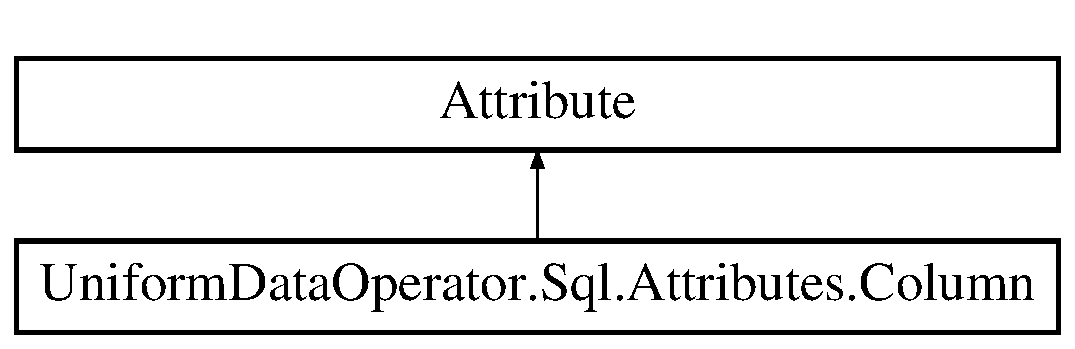
\includegraphics[height=2.000000cm]{d9/d44/class_uniform_data_operator_1_1_sql_1_1_attributes_1_1_column}
\end{center}
\end{figure}
\subsection*{Public Member Functions}
\begin{DoxyCompactItemize}
\item 
\mbox{\hyperlink{class_uniform_data_operator_1_1_sql_1_1_attributes_1_1_column_a8ff9ad5c1502f9e64f08273d7d4a50f6}{Column}} (string \mbox{\hyperlink{class_uniform_data_operator_1_1_sql_1_1_attributes_1_1_column_af17925ba835ca424a854689016526e93}{title}}, Db\+Type \mbox{\hyperlink{class_uniform_data_operator_1_1_sql_1_1_attributes_1_1_column_ad42f01b863fcea9172fc5efe2b8a0834}{type}})
\begin{DoxyCompactList}\small\item\em Init column. \end{DoxyCompactList}\item 
override string \mbox{\hyperlink{class_uniform_data_operator_1_1_sql_1_1_attributes_1_1_column_a20c1639a185fb8f5c3cd09927e79d672}{To\+String}} ()
\begin{DoxyCompactList}\small\item\em Converting column to string view. \end{DoxyCompactList}\end{DoxyCompactItemize}
\subsection*{Static Public Member Functions}
\begin{DoxyCompactItemize}
\item 
static implicit \mbox{\hyperlink{class_uniform_data_operator_1_1_sql_1_1_attributes_1_1_column_a2f2533d559fba4736f749a5eba9852f6}{operator string}} (\mbox{\hyperlink{class_uniform_data_operator_1_1_sql_1_1_attributes_1_1_column}{Column}} column)
\begin{DoxyCompactList}\small\item\em Converting column to string view. \end{DoxyCompactList}\item 
static void \mbox{\hyperlink{class_uniform_data_operator_1_1_sql_1_1_attributes_1_1_column_aa3e174a477fdbeaa14aff1c783c2b1f9}{Members\+Data\+To\+Command}} (ref object data, ref Db\+Command command, I\+Enumerable$<$ Member\+Info $>$ members)
\begin{DoxyCompactList}\small\item\em Adding members columns data to params. \end{DoxyCompactList}\item 
static void \mbox{\hyperlink{class_uniform_data_operator_1_1_sql_1_1_attributes_1_1_column_a7b8f106a53f21e586ef1f8f2ac5a43eb}{Members\+To\+Meta\+Lists}} (I\+Enumerable$<$ Member\+Info $>$ members, out List$<$ \mbox{\hyperlink{class_uniform_data_operator_1_1_sql_1_1_attributes_1_1_column}{Column}} $>$ columns, out List$<$ string $>$ variables)
\begin{DoxyCompactList}\small\item\em Converting collection of members to lists that contain\textquotesingle{}s splited meta data suitable for queries. \end{DoxyCompactList}\end{DoxyCompactItemize}
\subsection*{Public Attributes}
\begin{DoxyCompactItemize}
\item 
string \mbox{\hyperlink{class_uniform_data_operator_1_1_sql_1_1_attributes_1_1_column_af17925ba835ca424a854689016526e93}{title}}
\begin{DoxyCompactList}\small\item\em Title of column in table. \end{DoxyCompactList}\item 
Db\+Type \mbox{\hyperlink{class_uniform_data_operator_1_1_sql_1_1_attributes_1_1_column_ad42f01b863fcea9172fc5efe2b8a0834}{type}}
\begin{DoxyCompactList}\small\item\em Type of column in table. \end{DoxyCompactList}\end{DoxyCompactItemize}


\subsection{Detailed Description}
Descriptro of data base table\textquotesingle{}s column. 



\subsection{Constructor \& Destructor Documentation}
\mbox{\Hypertarget{class_uniform_data_operator_1_1_sql_1_1_attributes_1_1_column_a8ff9ad5c1502f9e64f08273d7d4a50f6}\label{class_uniform_data_operator_1_1_sql_1_1_attributes_1_1_column_a8ff9ad5c1502f9e64f08273d7d4a50f6}} 
\index{Uniform\+Data\+Operator\+::\+Sql\+::\+Attributes\+::\+Column@{Uniform\+Data\+Operator\+::\+Sql\+::\+Attributes\+::\+Column}!Column@{Column}}
\index{Column@{Column}!Uniform\+Data\+Operator\+::\+Sql\+::\+Attributes\+::\+Column@{Uniform\+Data\+Operator\+::\+Sql\+::\+Attributes\+::\+Column}}
\subsubsection{\texorpdfstring{Column()}{Column()}}
{\footnotesize\ttfamily Uniform\+Data\+Operator.\+Sql.\+Attributes.\+Column.\+Column (\begin{DoxyParamCaption}\item[{string}]{title,  }\item[{Db\+Type}]{type }\end{DoxyParamCaption})}



Init column. 


\begin{DoxyParams}{Parameters}
{\em title} & Title of column in table.\\
\hline
{\em type} & Type of column in table.\\
\hline
\end{DoxyParams}


\subsection{Member Function Documentation}
\mbox{\Hypertarget{class_uniform_data_operator_1_1_sql_1_1_attributes_1_1_column_aa3e174a477fdbeaa14aff1c783c2b1f9}\label{class_uniform_data_operator_1_1_sql_1_1_attributes_1_1_column_aa3e174a477fdbeaa14aff1c783c2b1f9}} 
\index{Uniform\+Data\+Operator\+::\+Sql\+::\+Attributes\+::\+Column@{Uniform\+Data\+Operator\+::\+Sql\+::\+Attributes\+::\+Column}!Members\+Data\+To\+Command@{Members\+Data\+To\+Command}}
\index{Members\+Data\+To\+Command@{Members\+Data\+To\+Command}!Uniform\+Data\+Operator\+::\+Sql\+::\+Attributes\+::\+Column@{Uniform\+Data\+Operator\+::\+Sql\+::\+Attributes\+::\+Column}}
\subsubsection{\texorpdfstring{Members\+Data\+To\+Command()}{MembersDataToCommand()}}
{\footnotesize\ttfamily static void Uniform\+Data\+Operator.\+Sql.\+Attributes.\+Column.\+Members\+Data\+To\+Command (\begin{DoxyParamCaption}\item[{ref object}]{data,  }\item[{ref Db\+Command}]{command,  }\item[{I\+Enumerable$<$ Member\+Info $>$}]{members }\end{DoxyParamCaption})\hspace{0.3cm}{\ttfamily [static]}}



Adding members columns data to params. 


\begin{DoxyParams}{Parameters}
{\em data} & Object that contains values relative to members.\\
\hline
{\em command} & Command objects that would share values.\\
\hline
{\em members} & Members that with defined \mbox{\hyperlink{class_uniform_data_operator_1_1_sql_1_1_attributes_1_1_column}{Column}} attribute that would be stored to command.\\
\hline
\end{DoxyParams}
\mbox{\Hypertarget{class_uniform_data_operator_1_1_sql_1_1_attributes_1_1_column_a7b8f106a53f21e586ef1f8f2ac5a43eb}\label{class_uniform_data_operator_1_1_sql_1_1_attributes_1_1_column_a7b8f106a53f21e586ef1f8f2ac5a43eb}} 
\index{Uniform\+Data\+Operator\+::\+Sql\+::\+Attributes\+::\+Column@{Uniform\+Data\+Operator\+::\+Sql\+::\+Attributes\+::\+Column}!Members\+To\+Meta\+Lists@{Members\+To\+Meta\+Lists}}
\index{Members\+To\+Meta\+Lists@{Members\+To\+Meta\+Lists}!Uniform\+Data\+Operator\+::\+Sql\+::\+Attributes\+::\+Column@{Uniform\+Data\+Operator\+::\+Sql\+::\+Attributes\+::\+Column}}
\subsubsection{\texorpdfstring{Members\+To\+Meta\+Lists()}{MembersToMetaLists()}}
{\footnotesize\ttfamily static void Uniform\+Data\+Operator.\+Sql.\+Attributes.\+Column.\+Members\+To\+Meta\+Lists (\begin{DoxyParamCaption}\item[{I\+Enumerable$<$ Member\+Info $>$}]{members,  }\item[{out List$<$ \mbox{\hyperlink{class_uniform_data_operator_1_1_sql_1_1_attributes_1_1_column}{Column}} $>$}]{columns,  }\item[{out List$<$ string $>$}]{variables }\end{DoxyParamCaption})\hspace{0.3cm}{\ttfamily [static]}}



Converting collection of members to lists that contain\textquotesingle{}s splited meta data suitable for queries. 


\begin{DoxyParams}{Parameters}
{\em members} & Source collection of memers.\\
\hline
{\em columns} & List that contains all detected columns descriptors.\\
\hline
{\em variables} & List that contains names of local variables in format allowed to internal queries generators.\\
\hline
\end{DoxyParams}
\mbox{\Hypertarget{class_uniform_data_operator_1_1_sql_1_1_attributes_1_1_column_a2f2533d559fba4736f749a5eba9852f6}\label{class_uniform_data_operator_1_1_sql_1_1_attributes_1_1_column_a2f2533d559fba4736f749a5eba9852f6}} 
\index{Uniform\+Data\+Operator\+::\+Sql\+::\+Attributes\+::\+Column@{Uniform\+Data\+Operator\+::\+Sql\+::\+Attributes\+::\+Column}!operator string@{operator string}}
\index{operator string@{operator string}!Uniform\+Data\+Operator\+::\+Sql\+::\+Attributes\+::\+Column@{Uniform\+Data\+Operator\+::\+Sql\+::\+Attributes\+::\+Column}}
\subsubsection{\texorpdfstring{operator string()}{operator string()}}
{\footnotesize\ttfamily static implicit Uniform\+Data\+Operator.\+Sql.\+Attributes.\+Column.\+operator string (\begin{DoxyParamCaption}\item[{\mbox{\hyperlink{class_uniform_data_operator_1_1_sql_1_1_attributes_1_1_column}{Column}}}]{column }\end{DoxyParamCaption})\hspace{0.3cm}{\ttfamily [static]}}



Converting column to string view. 


\begin{DoxyParams}{Parameters}
{\em column} & Input column.\\
\hline
\end{DoxyParams}
\mbox{\Hypertarget{class_uniform_data_operator_1_1_sql_1_1_attributes_1_1_column_a20c1639a185fb8f5c3cd09927e79d672}\label{class_uniform_data_operator_1_1_sql_1_1_attributes_1_1_column_a20c1639a185fb8f5c3cd09927e79d672}} 
\index{Uniform\+Data\+Operator\+::\+Sql\+::\+Attributes\+::\+Column@{Uniform\+Data\+Operator\+::\+Sql\+::\+Attributes\+::\+Column}!To\+String@{To\+String}}
\index{To\+String@{To\+String}!Uniform\+Data\+Operator\+::\+Sql\+::\+Attributes\+::\+Column@{Uniform\+Data\+Operator\+::\+Sql\+::\+Attributes\+::\+Column}}
\subsubsection{\texorpdfstring{To\+String()}{ToString()}}
{\footnotesize\ttfamily override string Uniform\+Data\+Operator.\+Sql.\+Attributes.\+Column.\+To\+String (\begin{DoxyParamCaption}{ }\end{DoxyParamCaption})}



Converting column to string view. 

\begin{DoxyReturn}{Returns}
Tielt of column.
\end{DoxyReturn}


\subsection{Member Data Documentation}
\mbox{\Hypertarget{class_uniform_data_operator_1_1_sql_1_1_attributes_1_1_column_af17925ba835ca424a854689016526e93}\label{class_uniform_data_operator_1_1_sql_1_1_attributes_1_1_column_af17925ba835ca424a854689016526e93}} 
\index{Uniform\+Data\+Operator\+::\+Sql\+::\+Attributes\+::\+Column@{Uniform\+Data\+Operator\+::\+Sql\+::\+Attributes\+::\+Column}!title@{title}}
\index{title@{title}!Uniform\+Data\+Operator\+::\+Sql\+::\+Attributes\+::\+Column@{Uniform\+Data\+Operator\+::\+Sql\+::\+Attributes\+::\+Column}}
\subsubsection{\texorpdfstring{title}{title}}
{\footnotesize\ttfamily string Uniform\+Data\+Operator.\+Sql.\+Attributes.\+Column.\+title}



Title of column in table. 

\mbox{\Hypertarget{class_uniform_data_operator_1_1_sql_1_1_attributes_1_1_column_ad42f01b863fcea9172fc5efe2b8a0834}\label{class_uniform_data_operator_1_1_sql_1_1_attributes_1_1_column_ad42f01b863fcea9172fc5efe2b8a0834}} 
\index{Uniform\+Data\+Operator\+::\+Sql\+::\+Attributes\+::\+Column@{Uniform\+Data\+Operator\+::\+Sql\+::\+Attributes\+::\+Column}!type@{type}}
\index{type@{type}!Uniform\+Data\+Operator\+::\+Sql\+::\+Attributes\+::\+Column@{Uniform\+Data\+Operator\+::\+Sql\+::\+Attributes\+::\+Column}}
\subsubsection{\texorpdfstring{type}{type}}
{\footnotesize\ttfamily Db\+Type Uniform\+Data\+Operator.\+Sql.\+Attributes.\+Column.\+type}



Type of column in table. 



The documentation for this class was generated from the following file\+:\begin{DoxyCompactItemize}
\item 
D\+:/\+Work/\+Git\+Hub/uniform-\/data-\/operator/\+S\+Q\+L/\+Attributes/Column.\+cs\end{DoxyCompactItemize}

\hypertarget{class_uniform_data_operator_1_1_sql_1_1_attributes_1_1_commentary}{}\section{Uniform\+Data\+Operator.\+Sql.\+Attributes.\+Commentary Class Reference}
\label{class_uniform_data_operator_1_1_sql_1_1_attributes_1_1_commentary}\index{Uniform\+Data\+Operator.\+Sql.\+Attributes.\+Commentary@{Uniform\+Data\+Operator.\+Sql.\+Attributes.\+Commentary}}


Add commentary to S\+QL table.  


Inheritance diagram for Uniform\+Data\+Operator.\+Sql.\+Attributes.\+Commentary\+:\begin{figure}[H]
\begin{center}
\leavevmode
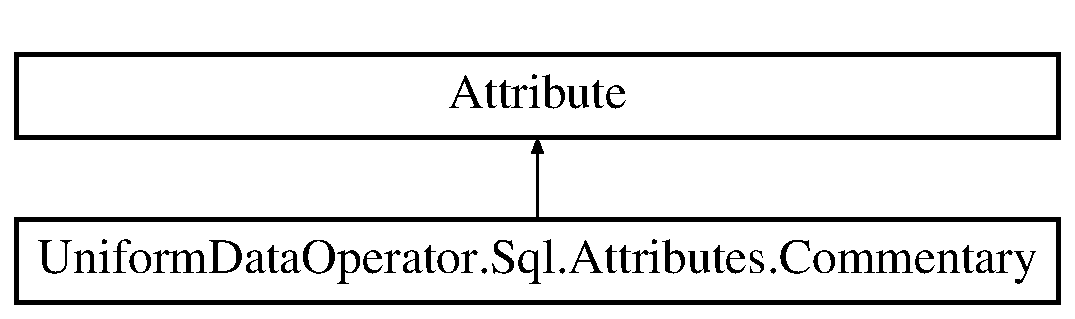
\includegraphics[height=2.000000cm]{d7/d35/class_uniform_data_operator_1_1_sql_1_1_attributes_1_1_commentary}
\end{center}
\end{figure}
\subsection*{Public Member Functions}
\begin{DoxyCompactItemize}
\item 
\mbox{\hyperlink{class_uniform_data_operator_1_1_sql_1_1_attributes_1_1_commentary_a32175c17c1db206f170ec84a8e83abd7}{Commentary}} (string \mbox{\hyperlink{class_uniform_data_operator_1_1_sql_1_1_attributes_1_1_commentary_a5cb463ba92cc10199d1a8ffb8c8729fd}{commentary}})
\begin{DoxyCompactList}\small\item\em Init commentary for column in table. \end{DoxyCompactList}\item 
override string \mbox{\hyperlink{class_uniform_data_operator_1_1_sql_1_1_attributes_1_1_commentary_a254d1f32018f1686b615a9ced5c0b1d5}{To\+String}} ()
\begin{DoxyCompactList}\small\item\em Return comment in string format. \end{DoxyCompactList}\end{DoxyCompactItemize}
\subsection*{Static Public Member Functions}
\begin{DoxyCompactItemize}
\item 
static implicit \mbox{\hyperlink{class_uniform_data_operator_1_1_sql_1_1_attributes_1_1_commentary_adb8a38bd8b9febe1222e715e7f7309d8}{operator string}} (\mbox{\hyperlink{class_uniform_data_operator_1_1_sql_1_1_attributes_1_1_commentary}{Commentary}} \mbox{\hyperlink{class_uniform_data_operator_1_1_sql_1_1_attributes_1_1_commentary_a5cb463ba92cc10199d1a8ffb8c8729fd}{commentary}})
\begin{DoxyCompactList}\small\item\em Return comment in string format. \end{DoxyCompactList}\end{DoxyCompactItemize}
\subsection*{Protected Attributes}
\begin{DoxyCompactItemize}
\item 
string \mbox{\hyperlink{class_uniform_data_operator_1_1_sql_1_1_attributes_1_1_commentary_a5cb463ba92cc10199d1a8ffb8c8729fd}{commentary}}
\begin{DoxyCompactList}\small\item\em \mbox{\hyperlink{class_uniform_data_operator_1_1_sql_1_1_attributes_1_1_commentary}{Commentary}} to the column. \end{DoxyCompactList}\end{DoxyCompactItemize}


\subsection{Detailed Description}
Add commentary to S\+QL table. 



\subsection{Constructor \& Destructor Documentation}
\mbox{\Hypertarget{class_uniform_data_operator_1_1_sql_1_1_attributes_1_1_commentary_a32175c17c1db206f170ec84a8e83abd7}\label{class_uniform_data_operator_1_1_sql_1_1_attributes_1_1_commentary_a32175c17c1db206f170ec84a8e83abd7}} 
\index{Uniform\+Data\+Operator\+::\+Sql\+::\+Attributes\+::\+Commentary@{Uniform\+Data\+Operator\+::\+Sql\+::\+Attributes\+::\+Commentary}!Commentary@{Commentary}}
\index{Commentary@{Commentary}!Uniform\+Data\+Operator\+::\+Sql\+::\+Attributes\+::\+Commentary@{Uniform\+Data\+Operator\+::\+Sql\+::\+Attributes\+::\+Commentary}}
\subsubsection{\texorpdfstring{Commentary()}{Commentary()}}
{\footnotesize\ttfamily Uniform\+Data\+Operator.\+Sql.\+Attributes.\+Commentary.\+Commentary (\begin{DoxyParamCaption}\item[{string}]{commentary }\end{DoxyParamCaption})}



Init commentary for column in table. 


\begin{DoxyParams}{Parameters}
{\em commentary} & \mbox{\hyperlink{class_uniform_data_operator_1_1_sql_1_1_attributes_1_1_commentary}{Commentary}} to the column.\\
\hline
\end{DoxyParams}


\subsection{Member Function Documentation}
\mbox{\Hypertarget{class_uniform_data_operator_1_1_sql_1_1_attributes_1_1_commentary_adb8a38bd8b9febe1222e715e7f7309d8}\label{class_uniform_data_operator_1_1_sql_1_1_attributes_1_1_commentary_adb8a38bd8b9febe1222e715e7f7309d8}} 
\index{Uniform\+Data\+Operator\+::\+Sql\+::\+Attributes\+::\+Commentary@{Uniform\+Data\+Operator\+::\+Sql\+::\+Attributes\+::\+Commentary}!operator string@{operator string}}
\index{operator string@{operator string}!Uniform\+Data\+Operator\+::\+Sql\+::\+Attributes\+::\+Commentary@{Uniform\+Data\+Operator\+::\+Sql\+::\+Attributes\+::\+Commentary}}
\subsubsection{\texorpdfstring{operator string()}{operator string()}}
{\footnotesize\ttfamily static implicit Uniform\+Data\+Operator.\+Sql.\+Attributes.\+Commentary.\+operator string (\begin{DoxyParamCaption}\item[{\mbox{\hyperlink{class_uniform_data_operator_1_1_sql_1_1_attributes_1_1_commentary}{Commentary}}}]{commentary }\end{DoxyParamCaption})\hspace{0.3cm}{\ttfamily [static]}}



Return comment in string format. 


\begin{DoxyParams}{Parameters}
{\em commentary} & Input comment.\\
\hline
\end{DoxyParams}
\mbox{\Hypertarget{class_uniform_data_operator_1_1_sql_1_1_attributes_1_1_commentary_a254d1f32018f1686b615a9ced5c0b1d5}\label{class_uniform_data_operator_1_1_sql_1_1_attributes_1_1_commentary_a254d1f32018f1686b615a9ced5c0b1d5}} 
\index{Uniform\+Data\+Operator\+::\+Sql\+::\+Attributes\+::\+Commentary@{Uniform\+Data\+Operator\+::\+Sql\+::\+Attributes\+::\+Commentary}!To\+String@{To\+String}}
\index{To\+String@{To\+String}!Uniform\+Data\+Operator\+::\+Sql\+::\+Attributes\+::\+Commentary@{Uniform\+Data\+Operator\+::\+Sql\+::\+Attributes\+::\+Commentary}}
\subsubsection{\texorpdfstring{To\+String()}{ToString()}}
{\footnotesize\ttfamily override string Uniform\+Data\+Operator.\+Sql.\+Attributes.\+Commentary.\+To\+String (\begin{DoxyParamCaption}{ }\end{DoxyParamCaption})}



Return comment in string format. 

\begin{DoxyReturn}{Returns}
Comment in string format.
\end{DoxyReturn}


\subsection{Member Data Documentation}
\mbox{\Hypertarget{class_uniform_data_operator_1_1_sql_1_1_attributes_1_1_commentary_a5cb463ba92cc10199d1a8ffb8c8729fd}\label{class_uniform_data_operator_1_1_sql_1_1_attributes_1_1_commentary_a5cb463ba92cc10199d1a8ffb8c8729fd}} 
\index{Uniform\+Data\+Operator\+::\+Sql\+::\+Attributes\+::\+Commentary@{Uniform\+Data\+Operator\+::\+Sql\+::\+Attributes\+::\+Commentary}!commentary@{commentary}}
\index{commentary@{commentary}!Uniform\+Data\+Operator\+::\+Sql\+::\+Attributes\+::\+Commentary@{Uniform\+Data\+Operator\+::\+Sql\+::\+Attributes\+::\+Commentary}}
\subsubsection{\texorpdfstring{commentary}{commentary}}
{\footnotesize\ttfamily string Uniform\+Data\+Operator.\+Sql.\+Attributes.\+Commentary.\+commentary\hspace{0.3cm}{\ttfamily [protected]}}



\mbox{\hyperlink{class_uniform_data_operator_1_1_sql_1_1_attributes_1_1_commentary}{Commentary}} to the column. 



The documentation for this class was generated from the following file\+:\begin{DoxyCompactItemize}
\item 
D\+:/\+Work/\+Git\+Hub/uniform-\/data-\/operator/\+S\+Q\+L/\+Attributes/Commentary.\+cs\end{DoxyCompactItemize}

\hypertarget{class_uniform_data_operator_1_1_sql_1_1_attributes_1_1_modifiers_1_1_d_b_path_override}{}\section{Uniform\+Data\+Operator.\+Sql.\+Attributes.\+Modifiers.\+D\+B\+Path\+Override Class Reference}
\label{class_uniform_data_operator_1_1_sql_1_1_attributes_1_1_modifiers_1_1_d_b_path_override}\index{Uniform\+Data\+Operator.\+Sql.\+Attributes.\+Modifiers.\+D\+B\+Path\+Override@{Uniform\+Data\+Operator.\+Sql.\+Attributes.\+Modifiers.\+D\+B\+Path\+Override}}


Overriding data base path to member in attributes that looking for this attribute.  


Inheritance diagram for Uniform\+Data\+Operator.\+Sql.\+Attributes.\+Modifiers.\+D\+B\+Path\+Override\+:\begin{figure}[H]
\begin{center}
\leavevmode
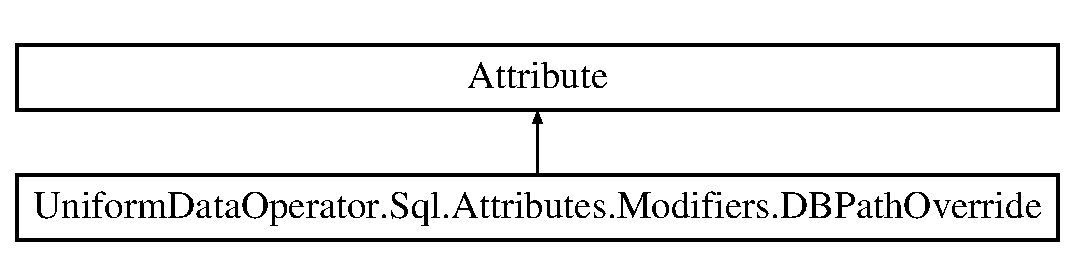
\includegraphics[height=2.000000cm]{d0/daf/class_uniform_data_operator_1_1_sql_1_1_attributes_1_1_modifiers_1_1_d_b_path_override}
\end{center}
\end{figure}
\subsection*{Static Public Member Functions}
\begin{DoxyCompactItemize}
\item 
static bool \mbox{\hyperlink{class_uniform_data_operator_1_1_sql_1_1_attributes_1_1_modifiers_1_1_d_b_path_override_aa7601220e39d8a68e911e4215bf94cb5}{Try\+To\+Get\+Valid\+Override$<$ T $>$}} (Member\+Info member, out \mbox{\hyperlink{class_uniform_data_operator_1_1_sql_1_1_attributes_1_1_modifiers_1_1_d_b_path_override}{D\+B\+Path\+Override}} output)
\begin{DoxyCompactList}\small\item\em Looking for path overriding attribute suitable for specified member and assking attribute. \end{DoxyCompactList}\end{DoxyCompactItemize}
\subsection*{Public Attributes}
\begin{DoxyCompactItemize}
\item 
Type \mbox{\hyperlink{class_uniform_data_operator_1_1_sql_1_1_attributes_1_1_modifiers_1_1_d_b_path_override_adab73111e55f6fe699e34e19a1b86335}{target\+Attribute}}
\begin{DoxyCompactList}\small\item\em Type of attribute that would be affected by this overriding. If null that overriding would be applied to all who looking for. \end{DoxyCompactList}\item 
string \mbox{\hyperlink{class_uniform_data_operator_1_1_sql_1_1_attributes_1_1_modifiers_1_1_d_b_path_override_ac9dae1ac46998a11f6b037dc72639e53}{schema}}
\begin{DoxyCompactList}\small\item\em Name of schema that would be used during mentoing of this member in queries if possible. Will be skiped if null. \end{DoxyCompactList}\item 
string \mbox{\hyperlink{class_uniform_data_operator_1_1_sql_1_1_attributes_1_1_modifiers_1_1_d_b_path_override_abc320e5e035c21997a54aad8e4df52b7}{table}}
\begin{DoxyCompactList}\small\item\em Name of table that would be used during mentoing of this member in queries if possible. Will be skiped if null. \end{DoxyCompactList}\item 
string \mbox{\hyperlink{class_uniform_data_operator_1_1_sql_1_1_attributes_1_1_modifiers_1_1_d_b_path_override_afb1db0b618dd444cdaaab366172e4af1}{column}}
\begin{DoxyCompactList}\small\item\em Name of column that would be used during mentoing of this member in queries if possible. Will be skiped if null. \end{DoxyCompactList}\end{DoxyCompactItemize}


\subsection{Detailed Description}
Overriding data base path to member in attributes that looking for this attribute. 



\subsection{Member Function Documentation}
\mbox{\Hypertarget{class_uniform_data_operator_1_1_sql_1_1_attributes_1_1_modifiers_1_1_d_b_path_override_aa7601220e39d8a68e911e4215bf94cb5}\label{class_uniform_data_operator_1_1_sql_1_1_attributes_1_1_modifiers_1_1_d_b_path_override_aa7601220e39d8a68e911e4215bf94cb5}} 
\index{Uniform\+Data\+Operator\+::\+Sql\+::\+Attributes\+::\+Modifiers\+::\+D\+B\+Path\+Override@{Uniform\+Data\+Operator\+::\+Sql\+::\+Attributes\+::\+Modifiers\+::\+D\+B\+Path\+Override}!Try\+To\+Get\+Valid\+Override$<$ T $>$@{Try\+To\+Get\+Valid\+Override$<$ T $>$}}
\index{Try\+To\+Get\+Valid\+Override$<$ T $>$@{Try\+To\+Get\+Valid\+Override$<$ T $>$}!Uniform\+Data\+Operator\+::\+Sql\+::\+Attributes\+::\+Modifiers\+::\+D\+B\+Path\+Override@{Uniform\+Data\+Operator\+::\+Sql\+::\+Attributes\+::\+Modifiers\+::\+D\+B\+Path\+Override}}
\subsubsection{\texorpdfstring{Try\+To\+Get\+Valid\+Override$<$ T $>$()}{TryToGetValidOverride< T >()}}
{\footnotesize\ttfamily static bool Uniform\+Data\+Operator.\+Sql.\+Attributes.\+Modifiers.\+D\+B\+Path\+Override.\+Try\+To\+Get\+Valid\+Override$<$ T $>$ (\begin{DoxyParamCaption}\item[{Member\+Info}]{member,  }\item[{out \mbox{\hyperlink{class_uniform_data_operator_1_1_sql_1_1_attributes_1_1_modifiers_1_1_d_b_path_override}{D\+B\+Path\+Override}}}]{output }\end{DoxyParamCaption})\hspace{0.3cm}{\ttfamily [static]}}



Looking for path overriding attribute suitable for specified member and assking attribute. 


\begin{DoxyTemplParams}{Template Parameters}
{\em T} & Attribute that would be locked as an overriding target\\
\hline
\end{DoxyTemplParams}

\begin{DoxyParams}{Parameters}
{\em member} & Member that could contains attribute.\\
\hline
{\em output} & Suitable override attribute.\\
\hline
\end{DoxyParams}
\begin{DoxyReturn}{Returns}
Result of operation.
\end{DoxyReturn}
\begin{Desc}
\item[Type Constraints]\begin{description}
\item[{\em T} : {\em Attribute}]\end{description}
\end{Desc}


\subsection{Member Data Documentation}
\mbox{\Hypertarget{class_uniform_data_operator_1_1_sql_1_1_attributes_1_1_modifiers_1_1_d_b_path_override_afb1db0b618dd444cdaaab366172e4af1}\label{class_uniform_data_operator_1_1_sql_1_1_attributes_1_1_modifiers_1_1_d_b_path_override_afb1db0b618dd444cdaaab366172e4af1}} 
\index{Uniform\+Data\+Operator\+::\+Sql\+::\+Attributes\+::\+Modifiers\+::\+D\+B\+Path\+Override@{Uniform\+Data\+Operator\+::\+Sql\+::\+Attributes\+::\+Modifiers\+::\+D\+B\+Path\+Override}!column@{column}}
\index{column@{column}!Uniform\+Data\+Operator\+::\+Sql\+::\+Attributes\+::\+Modifiers\+::\+D\+B\+Path\+Override@{Uniform\+Data\+Operator\+::\+Sql\+::\+Attributes\+::\+Modifiers\+::\+D\+B\+Path\+Override}}
\subsubsection{\texorpdfstring{column}{column}}
{\footnotesize\ttfamily string Uniform\+Data\+Operator.\+Sql.\+Attributes.\+Modifiers.\+D\+B\+Path\+Override.\+column}



Name of column that would be used during mentoing of this member in queries if possible. Will be skiped if null. 

\mbox{\Hypertarget{class_uniform_data_operator_1_1_sql_1_1_attributes_1_1_modifiers_1_1_d_b_path_override_ac9dae1ac46998a11f6b037dc72639e53}\label{class_uniform_data_operator_1_1_sql_1_1_attributes_1_1_modifiers_1_1_d_b_path_override_ac9dae1ac46998a11f6b037dc72639e53}} 
\index{Uniform\+Data\+Operator\+::\+Sql\+::\+Attributes\+::\+Modifiers\+::\+D\+B\+Path\+Override@{Uniform\+Data\+Operator\+::\+Sql\+::\+Attributes\+::\+Modifiers\+::\+D\+B\+Path\+Override}!schema@{schema}}
\index{schema@{schema}!Uniform\+Data\+Operator\+::\+Sql\+::\+Attributes\+::\+Modifiers\+::\+D\+B\+Path\+Override@{Uniform\+Data\+Operator\+::\+Sql\+::\+Attributes\+::\+Modifiers\+::\+D\+B\+Path\+Override}}
\subsubsection{\texorpdfstring{schema}{schema}}
{\footnotesize\ttfamily string Uniform\+Data\+Operator.\+Sql.\+Attributes.\+Modifiers.\+D\+B\+Path\+Override.\+schema}



Name of schema that would be used during mentoing of this member in queries if possible. Will be skiped if null. 

\mbox{\Hypertarget{class_uniform_data_operator_1_1_sql_1_1_attributes_1_1_modifiers_1_1_d_b_path_override_abc320e5e035c21997a54aad8e4df52b7}\label{class_uniform_data_operator_1_1_sql_1_1_attributes_1_1_modifiers_1_1_d_b_path_override_abc320e5e035c21997a54aad8e4df52b7}} 
\index{Uniform\+Data\+Operator\+::\+Sql\+::\+Attributes\+::\+Modifiers\+::\+D\+B\+Path\+Override@{Uniform\+Data\+Operator\+::\+Sql\+::\+Attributes\+::\+Modifiers\+::\+D\+B\+Path\+Override}!table@{table}}
\index{table@{table}!Uniform\+Data\+Operator\+::\+Sql\+::\+Attributes\+::\+Modifiers\+::\+D\+B\+Path\+Override@{Uniform\+Data\+Operator\+::\+Sql\+::\+Attributes\+::\+Modifiers\+::\+D\+B\+Path\+Override}}
\subsubsection{\texorpdfstring{table}{table}}
{\footnotesize\ttfamily string Uniform\+Data\+Operator.\+Sql.\+Attributes.\+Modifiers.\+D\+B\+Path\+Override.\+table}



Name of table that would be used during mentoing of this member in queries if possible. Will be skiped if null. 

\mbox{\Hypertarget{class_uniform_data_operator_1_1_sql_1_1_attributes_1_1_modifiers_1_1_d_b_path_override_adab73111e55f6fe699e34e19a1b86335}\label{class_uniform_data_operator_1_1_sql_1_1_attributes_1_1_modifiers_1_1_d_b_path_override_adab73111e55f6fe699e34e19a1b86335}} 
\index{Uniform\+Data\+Operator\+::\+Sql\+::\+Attributes\+::\+Modifiers\+::\+D\+B\+Path\+Override@{Uniform\+Data\+Operator\+::\+Sql\+::\+Attributes\+::\+Modifiers\+::\+D\+B\+Path\+Override}!target\+Attribute@{target\+Attribute}}
\index{target\+Attribute@{target\+Attribute}!Uniform\+Data\+Operator\+::\+Sql\+::\+Attributes\+::\+Modifiers\+::\+D\+B\+Path\+Override@{Uniform\+Data\+Operator\+::\+Sql\+::\+Attributes\+::\+Modifiers\+::\+D\+B\+Path\+Override}}
\subsubsection{\texorpdfstring{target\+Attribute}{targetAttribute}}
{\footnotesize\ttfamily Type Uniform\+Data\+Operator.\+Sql.\+Attributes.\+Modifiers.\+D\+B\+Path\+Override.\+target\+Attribute}



Type of attribute that would be affected by this overriding. If null that overriding would be applied to all who looking for. 



The documentation for this class was generated from the following file\+:\begin{DoxyCompactItemize}
\item 
D\+:/\+Work/\+Git\+Hub/uniform-\/data-\/operator/\+S\+Q\+L/\+Attributes/\+Modifiers/D\+B\+Path\+Override.\+cs\end{DoxyCompactItemize}

\hypertarget{class_uniform_data_operator_1_1_sql_1_1_attributes_1_1_default}{}\section{Uniform\+Data\+Operator.\+Sql.\+Attributes.\+Default Class Reference}
\label{class_uniform_data_operator_1_1_sql_1_1_attributes_1_1_default}\index{Uniform\+Data\+Operator.\+Sql.\+Attributes.\+Default@{Uniform\+Data\+Operator.\+Sql.\+Attributes.\+Default}}


Add default valu to the field.  


Inheritance diagram for Uniform\+Data\+Operator.\+Sql.\+Attributes.\+Default\+:\begin{figure}[H]
\begin{center}
\leavevmode
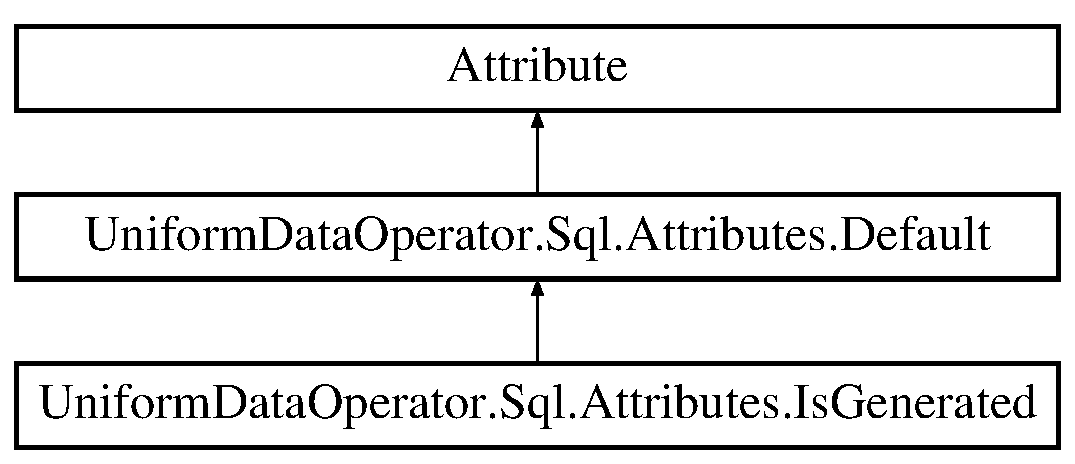
\includegraphics[height=3.000000cm]{d6/df9/class_uniform_data_operator_1_1_sql_1_1_attributes_1_1_default}
\end{center}
\end{figure}
\subsection*{Public Member Functions}
\begin{DoxyCompactItemize}
\item 
\mbox{\hyperlink{class_uniform_data_operator_1_1_sql_1_1_attributes_1_1_default_a9b6f3f42eccfc683466b3b8740e57212}{Default}} (string \mbox{\hyperlink{class_uniform_data_operator_1_1_sql_1_1_attributes_1_1_default_a1ba564b7f35af4395bafa39d6f5f69dc}{def\+Exp}})
\begin{DoxyCompactList}\small\item\em Init default value. \end{DoxyCompactList}\end{DoxyCompactItemize}
\subsection*{Public Attributes}
\begin{DoxyCompactItemize}
\item 
string \mbox{\hyperlink{class_uniform_data_operator_1_1_sql_1_1_attributes_1_1_default_a1ba564b7f35af4395bafa39d6f5f69dc}{def\+Exp}}
\begin{DoxyCompactList}\small\item\em \mbox{\hyperlink{class_uniform_data_operator_1_1_sql_1_1_attributes_1_1_default}{Default}} or Expression value. \end{DoxyCompactList}\end{DoxyCompactItemize}


\subsection{Detailed Description}
Add default valu to the field. 



\subsection{Constructor \& Destructor Documentation}
\mbox{\Hypertarget{class_uniform_data_operator_1_1_sql_1_1_attributes_1_1_default_a9b6f3f42eccfc683466b3b8740e57212}\label{class_uniform_data_operator_1_1_sql_1_1_attributes_1_1_default_a9b6f3f42eccfc683466b3b8740e57212}} 
\index{Uniform\+Data\+Operator\+::\+Sql\+::\+Attributes\+::\+Default@{Uniform\+Data\+Operator\+::\+Sql\+::\+Attributes\+::\+Default}!Default@{Default}}
\index{Default@{Default}!Uniform\+Data\+Operator\+::\+Sql\+::\+Attributes\+::\+Default@{Uniform\+Data\+Operator\+::\+Sql\+::\+Attributes\+::\+Default}}
\subsubsection{\texorpdfstring{Default()}{Default()}}
{\footnotesize\ttfamily Uniform\+Data\+Operator.\+Sql.\+Attributes.\+Default.\+Default (\begin{DoxyParamCaption}\item[{string}]{def\+Exp }\end{DoxyParamCaption})}



Init default value. 


\begin{DoxyParams}{Parameters}
{\em def\+Exp} & \mbox{\hyperlink{class_uniform_data_operator_1_1_sql_1_1_attributes_1_1_default}{Default}} or Expression value.\\
\hline
\end{DoxyParams}


\subsection{Member Data Documentation}
\mbox{\Hypertarget{class_uniform_data_operator_1_1_sql_1_1_attributes_1_1_default_a1ba564b7f35af4395bafa39d6f5f69dc}\label{class_uniform_data_operator_1_1_sql_1_1_attributes_1_1_default_a1ba564b7f35af4395bafa39d6f5f69dc}} 
\index{Uniform\+Data\+Operator\+::\+Sql\+::\+Attributes\+::\+Default@{Uniform\+Data\+Operator\+::\+Sql\+::\+Attributes\+::\+Default}!def\+Exp@{def\+Exp}}
\index{def\+Exp@{def\+Exp}!Uniform\+Data\+Operator\+::\+Sql\+::\+Attributes\+::\+Default@{Uniform\+Data\+Operator\+::\+Sql\+::\+Attributes\+::\+Default}}
\subsubsection{\texorpdfstring{def\+Exp}{defExp}}
{\footnotesize\ttfamily string Uniform\+Data\+Operator.\+Sql.\+Attributes.\+Default.\+def\+Exp}



\mbox{\hyperlink{class_uniform_data_operator_1_1_sql_1_1_attributes_1_1_default}{Default}} or Expression value. 



The documentation for this class was generated from the following file\+:\begin{DoxyCompactItemize}
\item 
D\+:/\+Work/\+Git\+Hub/uniform-\/data-\/operator/\+S\+Q\+L/\+Attributes/Default.\+cs\end{DoxyCompactItemize}

\hypertarget{class_uniform_data_operator_1_1_sql_1_1_attributes_1_1_is_auto_increment}{}\section{Uniform\+Data\+Operator.\+Sql.\+Attributes.\+Is\+Auto\+Increment Class Reference}
\label{class_uniform_data_operator_1_1_sql_1_1_attributes_1_1_is_auto_increment}\index{Uniform\+Data\+Operator.\+Sql.\+Attributes.\+Is\+Auto\+Increment@{Uniform\+Data\+Operator.\+Sql.\+Attributes.\+Is\+Auto\+Increment}}


Is value of this column would incremented relative to previous one during init.  


Inheritance diagram for Uniform\+Data\+Operator.\+Sql.\+Attributes.\+Is\+Auto\+Increment\+:\begin{figure}[H]
\begin{center}
\leavevmode
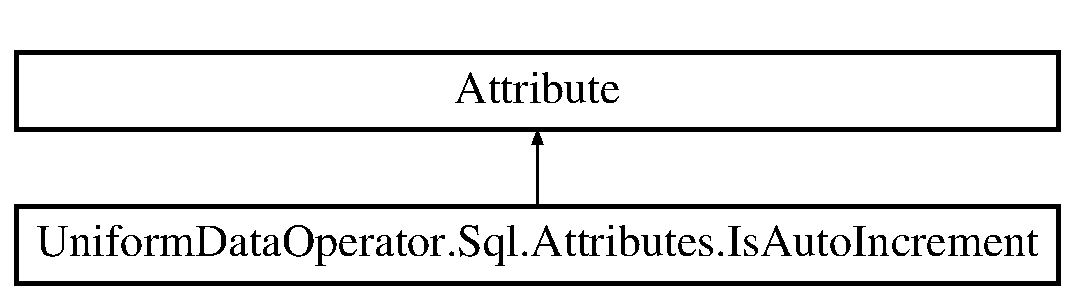
\includegraphics[height=2.000000cm]{d0/d59/class_uniform_data_operator_1_1_sql_1_1_attributes_1_1_is_auto_increment}
\end{center}
\end{figure}
\subsection*{Public Member Functions}
\begin{DoxyCompactItemize}
\item 
\mbox{\hyperlink{class_uniform_data_operator_1_1_sql_1_1_attributes_1_1_is_auto_increment_a738141c99b028f95fa9943dc385dd896}{Is\+Auto\+Increment}} ()
\begin{DoxyCompactList}\small\item\em Mark column as auto increament. \end{DoxyCompactList}\item 
\mbox{\Hypertarget{class_uniform_data_operator_1_1_sql_1_1_attributes_1_1_is_auto_increment_ad3e160ed18c83920560794d457cb9f97}\label{class_uniform_data_operator_1_1_sql_1_1_attributes_1_1_is_auto_increment_ad3e160ed18c83920560794d457cb9f97}} 
{\bfseries Is\+Auto\+Increment} (int ignore\+Value)
\end{DoxyCompactItemize}
\subsection*{Static Public Member Functions}
\begin{DoxyCompactItemize}
\item 
static Member\+Info \mbox{\hyperlink{class_uniform_data_operator_1_1_sql_1_1_attributes_1_1_is_auto_increment_ac254039f081903e685e116ec6993f9db}{Get\+Ignorable}} (ref object data)
\begin{DoxyCompactList}\small\item\em Trying to find member with defined \mbox{\hyperlink{class_uniform_data_operator_1_1_sql_1_1_attributes_1_1_is_auto_increment}{Is\+Auto\+Increment}} attribute in collection. If found, comparing it\textquotesingle{}s value with ignorable one. \end{DoxyCompactList}\item 
static Member\+Info \mbox{\hyperlink{class_uniform_data_operator_1_1_sql_1_1_attributes_1_1_is_auto_increment_ac662ab14322c8114855cb22e5395ab56}{Get\+Ignorable}} (ref object data, I\+Enumerable$<$ Member\+Info $>$ members)
\begin{DoxyCompactList}\small\item\em Trying to find member with defined \mbox{\hyperlink{class_uniform_data_operator_1_1_sql_1_1_attributes_1_1_is_auto_increment}{Is\+Auto\+Increment}} attribute in collection. If found, comparing it\textquotesingle{}s value with ignorable one. \end{DoxyCompactList}\end{DoxyCompactItemize}
\subsection*{Public Attributes}
\begin{DoxyCompactItemize}
\item 
\mbox{\Hypertarget{class_uniform_data_operator_1_1_sql_1_1_attributes_1_1_is_auto_increment_a3d14551782db0a2825335c02058c4735}\label{class_uniform_data_operator_1_1_sql_1_1_attributes_1_1_is_auto_increment_a3d14551782db0a2825335c02058c4735}} 
int {\bfseries ignore\+Value} = -\/1
\end{DoxyCompactItemize}
\subsection*{Static Protected Member Functions}
\begin{DoxyCompactItemize}
\item 
static bool \mbox{\hyperlink{class_uniform_data_operator_1_1_sql_1_1_attributes_1_1_is_auto_increment_acea9a992c39c789aa6ac336d7240a7bc}{Is\+Int\+Like}} (Type type)
\begin{DoxyCompactList}\small\item\em Cheing does the type is seems like int. \end{DoxyCompactList}\end{DoxyCompactItemize}


\subsection{Detailed Description}
Is value of this column would incremented relative to previous one during init. 



\subsection{Constructor \& Destructor Documentation}
\mbox{\Hypertarget{class_uniform_data_operator_1_1_sql_1_1_attributes_1_1_is_auto_increment_a738141c99b028f95fa9943dc385dd896}\label{class_uniform_data_operator_1_1_sql_1_1_attributes_1_1_is_auto_increment_a738141c99b028f95fa9943dc385dd896}} 
\index{Uniform\+Data\+Operator\+::\+Sql\+::\+Attributes\+::\+Is\+Auto\+Increment@{Uniform\+Data\+Operator\+::\+Sql\+::\+Attributes\+::\+Is\+Auto\+Increment}!Is\+Auto\+Increment@{Is\+Auto\+Increment}}
\index{Is\+Auto\+Increment@{Is\+Auto\+Increment}!Uniform\+Data\+Operator\+::\+Sql\+::\+Attributes\+::\+Is\+Auto\+Increment@{Uniform\+Data\+Operator\+::\+Sql\+::\+Attributes\+::\+Is\+Auto\+Increment}}
\subsubsection{\texorpdfstring{Is\+Auto\+Increment()}{IsAutoIncrement()}}
{\footnotesize\ttfamily Uniform\+Data\+Operator.\+Sql.\+Attributes.\+Is\+Auto\+Increment.\+Is\+Auto\+Increment (\begin{DoxyParamCaption}{ }\end{DoxyParamCaption})}



Mark column as auto increament. 



\subsection{Member Function Documentation}
\mbox{\Hypertarget{class_uniform_data_operator_1_1_sql_1_1_attributes_1_1_is_auto_increment_ac254039f081903e685e116ec6993f9db}\label{class_uniform_data_operator_1_1_sql_1_1_attributes_1_1_is_auto_increment_ac254039f081903e685e116ec6993f9db}} 
\index{Uniform\+Data\+Operator\+::\+Sql\+::\+Attributes\+::\+Is\+Auto\+Increment@{Uniform\+Data\+Operator\+::\+Sql\+::\+Attributes\+::\+Is\+Auto\+Increment}!Get\+Ignorable@{Get\+Ignorable}}
\index{Get\+Ignorable@{Get\+Ignorable}!Uniform\+Data\+Operator\+::\+Sql\+::\+Attributes\+::\+Is\+Auto\+Increment@{Uniform\+Data\+Operator\+::\+Sql\+::\+Attributes\+::\+Is\+Auto\+Increment}}
\subsubsection{\texorpdfstring{Get\+Ignorable()}{GetIgnorable()}\hspace{0.1cm}{\footnotesize\ttfamily [1/2]}}
{\footnotesize\ttfamily static Member\+Info Uniform\+Data\+Operator.\+Sql.\+Attributes.\+Is\+Auto\+Increment.\+Get\+Ignorable (\begin{DoxyParamCaption}\item[{ref object}]{data }\end{DoxyParamCaption})\hspace{0.3cm}{\ttfamily [static]}}



Trying to find member with defined \mbox{\hyperlink{class_uniform_data_operator_1_1_sql_1_1_attributes_1_1_is_auto_increment}{Is\+Auto\+Increment}} attribute in collection. If found, comparing it\textquotesingle{}s value with ignorable one. 

Scaning all members that has defined \mbox{\hyperlink{class_uniform_data_operator_1_1_sql_1_1_attributes_1_1_column}{Column}} attribute. 


\begin{DoxyParams}{Parameters}
{\em data} & Object that contain member.\\
\hline
\end{DoxyParams}
\begin{DoxyReturn}{Returns}
Return member if value equal defined ignorable. Null if \mbox{\hyperlink{class_uniform_data_operator_1_1_sql_1_1_attributes_1_1_is_auto_increment}{Is\+Auto\+Increment}} not defined or object has not defaul value.
\end{DoxyReturn}
\mbox{\Hypertarget{class_uniform_data_operator_1_1_sql_1_1_attributes_1_1_is_auto_increment_ac662ab14322c8114855cb22e5395ab56}\label{class_uniform_data_operator_1_1_sql_1_1_attributes_1_1_is_auto_increment_ac662ab14322c8114855cb22e5395ab56}} 
\index{Uniform\+Data\+Operator\+::\+Sql\+::\+Attributes\+::\+Is\+Auto\+Increment@{Uniform\+Data\+Operator\+::\+Sql\+::\+Attributes\+::\+Is\+Auto\+Increment}!Get\+Ignorable@{Get\+Ignorable}}
\index{Get\+Ignorable@{Get\+Ignorable}!Uniform\+Data\+Operator\+::\+Sql\+::\+Attributes\+::\+Is\+Auto\+Increment@{Uniform\+Data\+Operator\+::\+Sql\+::\+Attributes\+::\+Is\+Auto\+Increment}}
\subsubsection{\texorpdfstring{Get\+Ignorable()}{GetIgnorable()}\hspace{0.1cm}{\footnotesize\ttfamily [2/2]}}
{\footnotesize\ttfamily static Member\+Info Uniform\+Data\+Operator.\+Sql.\+Attributes.\+Is\+Auto\+Increment.\+Get\+Ignorable (\begin{DoxyParamCaption}\item[{ref object}]{data,  }\item[{I\+Enumerable$<$ Member\+Info $>$}]{members }\end{DoxyParamCaption})\hspace{0.3cm}{\ttfamily [static]}}



Trying to find member with defined \mbox{\hyperlink{class_uniform_data_operator_1_1_sql_1_1_attributes_1_1_is_auto_increment}{Is\+Auto\+Increment}} attribute in collection. If found, comparing it\textquotesingle{}s value with ignorable one. 


\begin{DoxyParams}{Parameters}
{\em data} & Object that contain member.\\
\hline
{\em members} & List of members that would be checked for this object.\\
\hline
\end{DoxyParams}
\begin{DoxyReturn}{Returns}
Return member if value equal defined ignorable. Null if \mbox{\hyperlink{class_uniform_data_operator_1_1_sql_1_1_attributes_1_1_is_auto_increment}{Is\+Auto\+Increment}} not defined or object has not defaul value.
\end{DoxyReturn}
\mbox{\Hypertarget{class_uniform_data_operator_1_1_sql_1_1_attributes_1_1_is_auto_increment_acea9a992c39c789aa6ac336d7240a7bc}\label{class_uniform_data_operator_1_1_sql_1_1_attributes_1_1_is_auto_increment_acea9a992c39c789aa6ac336d7240a7bc}} 
\index{Uniform\+Data\+Operator\+::\+Sql\+::\+Attributes\+::\+Is\+Auto\+Increment@{Uniform\+Data\+Operator\+::\+Sql\+::\+Attributes\+::\+Is\+Auto\+Increment}!Is\+Int\+Like@{Is\+Int\+Like}}
\index{Is\+Int\+Like@{Is\+Int\+Like}!Uniform\+Data\+Operator\+::\+Sql\+::\+Attributes\+::\+Is\+Auto\+Increment@{Uniform\+Data\+Operator\+::\+Sql\+::\+Attributes\+::\+Is\+Auto\+Increment}}
\subsubsection{\texorpdfstring{Is\+Int\+Like()}{IsIntLike()}}
{\footnotesize\ttfamily static bool Uniform\+Data\+Operator.\+Sql.\+Attributes.\+Is\+Auto\+Increment.\+Is\+Int\+Like (\begin{DoxyParamCaption}\item[{Type}]{type }\end{DoxyParamCaption})\hspace{0.3cm}{\ttfamily [static]}, {\ttfamily [protected]}}



Cheing does the type is seems like int. 


\begin{DoxyParams}{Parameters}
{\em type} & Type that would be comparet to ints.\\
\hline
\end{DoxyParams}
\begin{DoxyReturn}{Returns}
Result of types commpession.
\end{DoxyReturn}


The documentation for this class was generated from the following file\+:\begin{DoxyCompactItemize}
\item 
D\+:/\+Work/\+Git\+Hub/uniform-\/data-\/operator/\+S\+Q\+L/\+Attributes/Is\+Auto\+Increment.\+cs\end{DoxyCompactItemize}

\hypertarget{class_uniform_data_operator_1_1_sql_1_1_attributes_1_1_is_binary}{}\section{Uniform\+Data\+Operator.\+Sql.\+Attributes.\+Is\+Binary Class Reference}
\label{class_uniform_data_operator_1_1_sql_1_1_attributes_1_1_is_binary}\index{Uniform\+Data\+Operator.\+Sql.\+Attributes.\+Is\+Binary@{Uniform\+Data\+Operator.\+Sql.\+Attributes.\+Is\+Binary}}


Is data would stored in binary format.  


Inheritance diagram for Uniform\+Data\+Operator.\+Sql.\+Attributes.\+Is\+Binary\+:\begin{figure}[H]
\begin{center}
\leavevmode
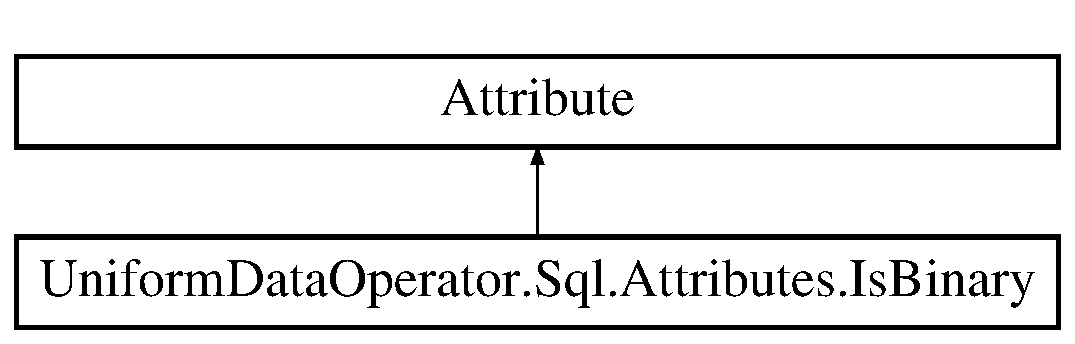
\includegraphics[height=2.000000cm]{d7/d13/class_uniform_data_operator_1_1_sql_1_1_attributes_1_1_is_binary}
\end{center}
\end{figure}


\subsection{Detailed Description}
Is data would stored in binary format. 



The documentation for this class was generated from the following file\+:\begin{DoxyCompactItemize}
\item 
D\+:/\+Work/\+Git\+Hub/uniform-\/data-\/operator/\+S\+Q\+L/\+Attributes/Is\+Binary.\+cs\end{DoxyCompactItemize}

\hypertarget{class_uniform_data_operator_1_1_sql_1_1_attributes_1_1_is_foreign_key}{}\section{Uniform\+Data\+Operator.\+Sql.\+Attributes.\+Is\+Foreign\+Key Class Reference}
\label{class_uniform_data_operator_1_1_sql_1_1_attributes_1_1_is_foreign_key}\index{Uniform\+Data\+Operator.\+Sql.\+Attributes.\+Is\+Foreign\+Key@{Uniform\+Data\+Operator.\+Sql.\+Attributes.\+Is\+Foreign\+Key}}


Mark fireld as foreign key to other column.  


Inheritance diagram for Uniform\+Data\+Operator.\+Sql.\+Attributes.\+Is\+Foreign\+Key\+:\begin{figure}[H]
\begin{center}
\leavevmode
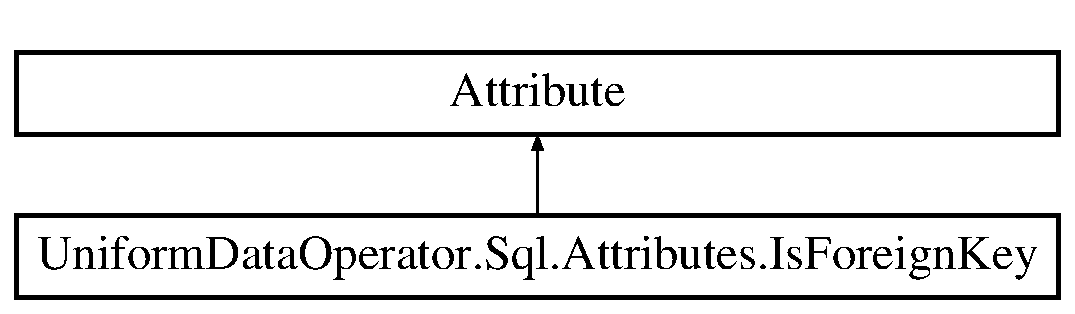
\includegraphics[height=2.000000cm]{de/db6/class_uniform_data_operator_1_1_sql_1_1_attributes_1_1_is_foreign_key}
\end{center}
\end{figure}
\subsection*{Public Types}
\begin{DoxyCompactItemize}
\item 
enum \mbox{\hyperlink{class_uniform_data_operator_1_1_sql_1_1_attributes_1_1_is_foreign_key_a6039622384e2bbd1aa386e326ee0f850}{Action}} \{ \mbox{\hyperlink{class_uniform_data_operator_1_1_sql_1_1_attributes_1_1_is_foreign_key_a6039622384e2bbd1aa386e326ee0f850a1e601ea653db1c729c9ee5746730fabe}{Action.\+No\+Action}}, 
\mbox{\hyperlink{class_uniform_data_operator_1_1_sql_1_1_attributes_1_1_is_foreign_key_a6039622384e2bbd1aa386e326ee0f850a2dc2b15e8b0ee7ed3fdd4cf53ad0a8c3}{Action.\+Cascade}}, 
\mbox{\hyperlink{class_uniform_data_operator_1_1_sql_1_1_attributes_1_1_is_foreign_key_a6039622384e2bbd1aa386e326ee0f850a034d70b46e41ec9d0306b0001e04cae7}{Action.\+Restrict}}, 
\mbox{\hyperlink{class_uniform_data_operator_1_1_sql_1_1_attributes_1_1_is_foreign_key_a6039622384e2bbd1aa386e326ee0f850a2ac481dd701d4f580b6b01eb34442e71}{Action.\+Set\+Null}}
 \}
\begin{DoxyCompactList}\small\item\em Action\textquotesingle{}s mode that would be used as reaction on event. \end{DoxyCompactList}\end{DoxyCompactItemize}
\subsection*{Public Member Functions}
\begin{DoxyCompactItemize}
\item 
\mbox{\hyperlink{class_uniform_data_operator_1_1_sql_1_1_attributes_1_1_is_foreign_key_a9c18736fa9035fb89c30cd5269d3ccc7}{Is\+Foreign\+Key}} (string \mbox{\hyperlink{class_uniform_data_operator_1_1_sql_1_1_attributes_1_1_is_foreign_key_a3adbb93b1e9ebb988b6fabf24e10991e}{schema}}, string \mbox{\hyperlink{class_uniform_data_operator_1_1_sql_1_1_attributes_1_1_is_foreign_key_ac480fc5f3f8ff86e0bb5877bab793e19}{table}}, string \mbox{\hyperlink{class_uniform_data_operator_1_1_sql_1_1_attributes_1_1_is_foreign_key_a8d14eef86991a9e1a187876626cbb70b}{column}})
\begin{DoxyCompactList}\small\item\em Configurate forgeign column reference. \end{DoxyCompactList}\item 
\mbox{\hyperlink{class_uniform_data_operator_1_1_sql_1_1_attributes_1_1_is_foreign_key_a9075c37e69d16608cd912c53726a683e}{Is\+Foreign\+Key}} (string \mbox{\hyperlink{class_uniform_data_operator_1_1_sql_1_1_attributes_1_1_is_foreign_key_a3adbb93b1e9ebb988b6fabf24e10991e}{schema}}, string \mbox{\hyperlink{class_uniform_data_operator_1_1_sql_1_1_attributes_1_1_is_foreign_key_ac480fc5f3f8ff86e0bb5877bab793e19}{table}}, string \mbox{\hyperlink{class_uniform_data_operator_1_1_sql_1_1_attributes_1_1_is_foreign_key_a8d14eef86991a9e1a187876626cbb70b}{column}}, \mbox{\hyperlink{class_uniform_data_operator_1_1_sql_1_1_attributes_1_1_is_foreign_key_a6039622384e2bbd1aa386e326ee0f850}{Action}} \mbox{\hyperlink{class_uniform_data_operator_1_1_sql_1_1_attributes_1_1_is_foreign_key_af70b31f4805f136d6a32b1fa33d9bbf6}{on\+Delete\+Command}}, \mbox{\hyperlink{class_uniform_data_operator_1_1_sql_1_1_attributes_1_1_is_foreign_key_a6039622384e2bbd1aa386e326ee0f850}{Action}} \mbox{\hyperlink{class_uniform_data_operator_1_1_sql_1_1_attributes_1_1_is_foreign_key_a3a45eb5c4419a10aafcc097c227bb794}{on\+Update\+Command}})
\begin{DoxyCompactList}\small\item\em Configurate forgeign column reference. \end{DoxyCompactList}\item 
string \mbox{\hyperlink{class_uniform_data_operator_1_1_sql_1_1_attributes_1_1_is_foreign_key_a0e272caef16165a57fee1499c7a94c8d}{F\+K\+Name}} (string self\+Table\+Name)
\begin{DoxyCompactList}\small\item\em Generate fk key name related to this column. \end{DoxyCompactList}\end{DoxyCompactItemize}
\subsection*{Static Public Member Functions}
\begin{DoxyCompactItemize}
\item 
static string \mbox{\hyperlink{class_uniform_data_operator_1_1_sql_1_1_attributes_1_1_is_foreign_key_a2673778ee437ef079b99d58636f7617b}{Action\+To\+Command}} (\mbox{\hyperlink{class_uniform_data_operator_1_1_sql_1_1_attributes_1_1_is_foreign_key_a6039622384e2bbd1aa386e326ee0f850}{Action}} action)
\begin{DoxyCompactList}\small\item\em Convert action to string format. \end{DoxyCompactList}\item 
static string \mbox{\hyperlink{class_uniform_data_operator_1_1_sql_1_1_attributes_1_1_is_foreign_key_a8d5c79de848dd87916ab946972db0188}{F\+K\+Index\+Declaration\+Command}} (Member\+Info member, string self\+Table\+Name)
\begin{DoxyCompactList}\small\item\em Return index init string suitable from forgeign key suitable for this column. Can auto detect modifers. \end{DoxyCompactList}\item 
static string \mbox{\hyperlink{class_uniform_data_operator_1_1_sql_1_1_attributes_1_1_is_foreign_key_a6becd6dc4bd6df070252b152a57f0152}{F\+K\+Index\+Declaration\+Command}} (\mbox{\hyperlink{class_uniform_data_operator_1_1_sql_1_1_attributes_1_1_column}{Column}} \mbox{\hyperlink{class_uniform_data_operator_1_1_sql_1_1_attributes_1_1_is_foreign_key_a8d14eef86991a9e1a187876626cbb70b}{column}}, \mbox{\hyperlink{class_uniform_data_operator_1_1_sql_1_1_attributes_1_1_is_foreign_key}{Is\+Foreign\+Key}} is\+Foreign\+Key, string self\+Table\+Name)
\begin{DoxyCompactList}\small\item\em Return index init string suitable from forgeign key suitable for this column. \end{DoxyCompactList}\item 
static void \mbox{\hyperlink{class_uniform_data_operator_1_1_sql_1_1_attributes_1_1_is_foreign_key_aba50c9adf8e4fac95010d26a17b54644}{Drop\+Indexator}} ()
\begin{DoxyCompactList}\small\item\em Clearing current index history. \end{DoxyCompactList}\item 
static string \mbox{\hyperlink{class_uniform_data_operator_1_1_sql_1_1_attributes_1_1_is_foreign_key_a795f460cb328bfe6d471134b4d48bedf}{Constrain\+Declaration\+Command}} (\mbox{\hyperlink{class_uniform_data_operator_1_1_sql_1_1_attributes_1_1_column}{Column}} \mbox{\hyperlink{class_uniform_data_operator_1_1_sql_1_1_attributes_1_1_is_foreign_key_a8d14eef86991a9e1a187876626cbb70b}{column}}, \mbox{\hyperlink{class_uniform_data_operator_1_1_sql_1_1_attributes_1_1_is_foreign_key}{Is\+Foreign\+Key}} is\+Foreign\+Key, string self\+Table\+Name)
\begin{DoxyCompactList}\small\item\em Generate init string from contrains related to this column. \end{DoxyCompactList}\item 
static string \mbox{\hyperlink{class_uniform_data_operator_1_1_sql_1_1_attributes_1_1_is_foreign_key_ae1dae3d2e36c2c38fe5306b42209ef74}{Constrain\+Declaration\+Command}} (Member\+Info member, string self\+Table\+Name)
\begin{DoxyCompactList}\small\item\em Generate init string from contrains related to this column. Can auto detect modifers. \end{DoxyCompactList}\end{DoxyCompactItemize}
\subsection*{Public Attributes}
\begin{DoxyCompactItemize}
\item 
string \mbox{\hyperlink{class_uniform_data_operator_1_1_sql_1_1_attributes_1_1_is_foreign_key_a3adbb93b1e9ebb988b6fabf24e10991e}{schema}}
\begin{DoxyCompactList}\small\item\em Name of foreign schema. \end{DoxyCompactList}\item 
string \mbox{\hyperlink{class_uniform_data_operator_1_1_sql_1_1_attributes_1_1_is_foreign_key_ac480fc5f3f8ff86e0bb5877bab793e19}{table}}
\begin{DoxyCompactList}\small\item\em Name of foreign table. \end{DoxyCompactList}\item 
string \mbox{\hyperlink{class_uniform_data_operator_1_1_sql_1_1_attributes_1_1_is_foreign_key_a8d14eef86991a9e1a187876626cbb70b}{column}}
\begin{DoxyCompactList}\small\item\em Name of foreign column. \end{DoxyCompactList}\item 
\mbox{\hyperlink{class_uniform_data_operator_1_1_sql_1_1_attributes_1_1_is_foreign_key_a6039622384e2bbd1aa386e326ee0f850}{Action}} \mbox{\hyperlink{class_uniform_data_operator_1_1_sql_1_1_attributes_1_1_is_foreign_key_af70b31f4805f136d6a32b1fa33d9bbf6}{on\+Delete\+Command}} = \mbox{\hyperlink{class_uniform_data_operator_1_1_sql_1_1_attributes_1_1_is_foreign_key_a6039622384e2bbd1aa386e326ee0f850a1e601ea653db1c729c9ee5746730fabe}{Action.\+No\+Action}}
\begin{DoxyCompactList}\small\item\em Command that would be applied in case of deleting. \end{DoxyCompactList}\item 
\mbox{\hyperlink{class_uniform_data_operator_1_1_sql_1_1_attributes_1_1_is_foreign_key_a6039622384e2bbd1aa386e326ee0f850}{Action}} \mbox{\hyperlink{class_uniform_data_operator_1_1_sql_1_1_attributes_1_1_is_foreign_key_a3a45eb5c4419a10aafcc097c227bb794}{on\+Update\+Command}} = \mbox{\hyperlink{class_uniform_data_operator_1_1_sql_1_1_attributes_1_1_is_foreign_key_a6039622384e2bbd1aa386e326ee0f850a1e601ea653db1c729c9ee5746730fabe}{Action.\+No\+Action}}
\begin{DoxyCompactList}\small\item\em Command that would be applied in case of updating. \end{DoxyCompactList}\end{DoxyCompactItemize}
\subsection*{Static Private Attributes}
\begin{DoxyCompactItemize}
\item 
\mbox{\Hypertarget{class_uniform_data_operator_1_1_sql_1_1_attributes_1_1_is_foreign_key_a30ca24c3d7b8c38c36a112c6d3d9db55}\label{class_uniform_data_operator_1_1_sql_1_1_attributes_1_1_is_foreign_key_a30ca24c3d7b8c38c36a112c6d3d9db55}} 
static readonly Hash\+Set$<$ string $>$ {\bfseries used\+Indexes} = new Hash\+Set$<$string$>$()
\end{DoxyCompactItemize}


\subsection{Detailed Description}
Mark fireld as foreign key to other column. 



\subsection{Member Enumeration Documentation}
\mbox{\Hypertarget{class_uniform_data_operator_1_1_sql_1_1_attributes_1_1_is_foreign_key_a6039622384e2bbd1aa386e326ee0f850}\label{class_uniform_data_operator_1_1_sql_1_1_attributes_1_1_is_foreign_key_a6039622384e2bbd1aa386e326ee0f850}} 
\index{Uniform\+Data\+Operator\+::\+Sql\+::\+Attributes\+::\+Is\+Foreign\+Key@{Uniform\+Data\+Operator\+::\+Sql\+::\+Attributes\+::\+Is\+Foreign\+Key}!Action@{Action}}
\index{Action@{Action}!Uniform\+Data\+Operator\+::\+Sql\+::\+Attributes\+::\+Is\+Foreign\+Key@{Uniform\+Data\+Operator\+::\+Sql\+::\+Attributes\+::\+Is\+Foreign\+Key}}
\subsubsection{\texorpdfstring{Action}{Action}}
{\footnotesize\ttfamily enum \mbox{\hyperlink{class_uniform_data_operator_1_1_sql_1_1_attributes_1_1_is_foreign_key_a6039622384e2bbd1aa386e326ee0f850}{Uniform\+Data\+Operator.\+Sql.\+Attributes.\+Is\+Foreign\+Key.\+Action}}\hspace{0.3cm}{\ttfamily [strong]}}



Action\textquotesingle{}s mode that would be used as reaction on event. 

\begin{DoxyEnumFields}{Enumerator}
\raisebox{\heightof{T}}[0pt][0pt]{\index{No\+Action@{No\+Action}!Uniform\+Data\+Operator\+::\+Sql\+::\+Attributes\+::\+Is\+Foreign\+Key@{Uniform\+Data\+Operator\+::\+Sql\+::\+Attributes\+::\+Is\+Foreign\+Key}}\index{Uniform\+Data\+Operator\+::\+Sql\+::\+Attributes\+::\+Is\+Foreign\+Key@{Uniform\+Data\+Operator\+::\+Sql\+::\+Attributes\+::\+Is\+Foreign\+Key}!No\+Action@{No\+Action}}}\mbox{\Hypertarget{class_uniform_data_operator_1_1_sql_1_1_attributes_1_1_is_foreign_key_a6039622384e2bbd1aa386e326ee0f850a1e601ea653db1c729c9ee5746730fabe}\label{class_uniform_data_operator_1_1_sql_1_1_attributes_1_1_is_foreign_key_a6039622384e2bbd1aa386e326ee0f850a1e601ea653db1c729c9ee5746730fabe}} 
No\+Action&Don\textquotesingle{}t do anything. \\
\hline

\raisebox{\heightof{T}}[0pt][0pt]{\index{Cascade@{Cascade}!Uniform\+Data\+Operator\+::\+Sql\+::\+Attributes\+::\+Is\+Foreign\+Key@{Uniform\+Data\+Operator\+::\+Sql\+::\+Attributes\+::\+Is\+Foreign\+Key}}\index{Uniform\+Data\+Operator\+::\+Sql\+::\+Attributes\+::\+Is\+Foreign\+Key@{Uniform\+Data\+Operator\+::\+Sql\+::\+Attributes\+::\+Is\+Foreign\+Key}!Cascade@{Cascade}}}\mbox{\Hypertarget{class_uniform_data_operator_1_1_sql_1_1_attributes_1_1_is_foreign_key_a6039622384e2bbd1aa386e326ee0f850a2dc2b15e8b0ee7ed3fdd4cf53ad0a8c3}\label{class_uniform_data_operator_1_1_sql_1_1_attributes_1_1_is_foreign_key_a6039622384e2bbd1aa386e326ee0f850a2dc2b15e8b0ee7ed3fdd4cf53ad0a8c3}} 
Cascade&Goins down by member and react all members in relative tables. \\
\hline

\raisebox{\heightof{T}}[0pt][0pt]{\index{Restrict@{Restrict}!Uniform\+Data\+Operator\+::\+Sql\+::\+Attributes\+::\+Is\+Foreign\+Key@{Uniform\+Data\+Operator\+::\+Sql\+::\+Attributes\+::\+Is\+Foreign\+Key}}\index{Uniform\+Data\+Operator\+::\+Sql\+::\+Attributes\+::\+Is\+Foreign\+Key@{Uniform\+Data\+Operator\+::\+Sql\+::\+Attributes\+::\+Is\+Foreign\+Key}!Restrict@{Restrict}}}\mbox{\Hypertarget{class_uniform_data_operator_1_1_sql_1_1_attributes_1_1_is_foreign_key_a6039622384e2bbd1aa386e326ee0f850a034d70b46e41ec9d0306b0001e04cae7}\label{class_uniform_data_operator_1_1_sql_1_1_attributes_1_1_is_foreign_key_a6039622384e2bbd1aa386e326ee0f850a034d70b46e41ec9d0306b0001e04cae7}} 
Restrict&Don\textquotesingle{}t do anything. \\
\hline

\raisebox{\heightof{T}}[0pt][0pt]{\index{Set\+Null@{Set\+Null}!Uniform\+Data\+Operator\+::\+Sql\+::\+Attributes\+::\+Is\+Foreign\+Key@{Uniform\+Data\+Operator\+::\+Sql\+::\+Attributes\+::\+Is\+Foreign\+Key}}\index{Uniform\+Data\+Operator\+::\+Sql\+::\+Attributes\+::\+Is\+Foreign\+Key@{Uniform\+Data\+Operator\+::\+Sql\+::\+Attributes\+::\+Is\+Foreign\+Key}!Set\+Null@{Set\+Null}}}\mbox{\Hypertarget{class_uniform_data_operator_1_1_sql_1_1_attributes_1_1_is_foreign_key_a6039622384e2bbd1aa386e326ee0f850a2ac481dd701d4f580b6b01eb34442e71}\label{class_uniform_data_operator_1_1_sql_1_1_attributes_1_1_is_foreign_key_a6039622384e2bbd1aa386e326ee0f850a2ac481dd701d4f580b6b01eb34442e71}} 
Set\+Null&Setting null to coulmn value. \\
\hline

\end{DoxyEnumFields}


\subsection{Constructor \& Destructor Documentation}
\mbox{\Hypertarget{class_uniform_data_operator_1_1_sql_1_1_attributes_1_1_is_foreign_key_a9c18736fa9035fb89c30cd5269d3ccc7}\label{class_uniform_data_operator_1_1_sql_1_1_attributes_1_1_is_foreign_key_a9c18736fa9035fb89c30cd5269d3ccc7}} 
\index{Uniform\+Data\+Operator\+::\+Sql\+::\+Attributes\+::\+Is\+Foreign\+Key@{Uniform\+Data\+Operator\+::\+Sql\+::\+Attributes\+::\+Is\+Foreign\+Key}!Is\+Foreign\+Key@{Is\+Foreign\+Key}}
\index{Is\+Foreign\+Key@{Is\+Foreign\+Key}!Uniform\+Data\+Operator\+::\+Sql\+::\+Attributes\+::\+Is\+Foreign\+Key@{Uniform\+Data\+Operator\+::\+Sql\+::\+Attributes\+::\+Is\+Foreign\+Key}}
\subsubsection{\texorpdfstring{Is\+Foreign\+Key()}{IsForeignKey()}\hspace{0.1cm}{\footnotesize\ttfamily [1/2]}}
{\footnotesize\ttfamily Uniform\+Data\+Operator.\+Sql.\+Attributes.\+Is\+Foreign\+Key.\+Is\+Foreign\+Key (\begin{DoxyParamCaption}\item[{string}]{schema,  }\item[{string}]{table,  }\item[{string}]{column }\end{DoxyParamCaption})}



Configurate forgeign column reference. 


\begin{DoxyParams}{Parameters}
{\em schema} & Name of foreign schema.\\
\hline
{\em table} & Name of foreign table.\\
\hline
{\em column} & Name of foreign column.\\
\hline
\end{DoxyParams}
\mbox{\Hypertarget{class_uniform_data_operator_1_1_sql_1_1_attributes_1_1_is_foreign_key_a9075c37e69d16608cd912c53726a683e}\label{class_uniform_data_operator_1_1_sql_1_1_attributes_1_1_is_foreign_key_a9075c37e69d16608cd912c53726a683e}} 
\index{Uniform\+Data\+Operator\+::\+Sql\+::\+Attributes\+::\+Is\+Foreign\+Key@{Uniform\+Data\+Operator\+::\+Sql\+::\+Attributes\+::\+Is\+Foreign\+Key}!Is\+Foreign\+Key@{Is\+Foreign\+Key}}
\index{Is\+Foreign\+Key@{Is\+Foreign\+Key}!Uniform\+Data\+Operator\+::\+Sql\+::\+Attributes\+::\+Is\+Foreign\+Key@{Uniform\+Data\+Operator\+::\+Sql\+::\+Attributes\+::\+Is\+Foreign\+Key}}
\subsubsection{\texorpdfstring{Is\+Foreign\+Key()}{IsForeignKey()}\hspace{0.1cm}{\footnotesize\ttfamily [2/2]}}
{\footnotesize\ttfamily Uniform\+Data\+Operator.\+Sql.\+Attributes.\+Is\+Foreign\+Key.\+Is\+Foreign\+Key (\begin{DoxyParamCaption}\item[{string}]{schema,  }\item[{string}]{table,  }\item[{string}]{column,  }\item[{\mbox{\hyperlink{class_uniform_data_operator_1_1_sql_1_1_attributes_1_1_is_foreign_key_a6039622384e2bbd1aa386e326ee0f850}{Action}}}]{on\+Delete\+Command,  }\item[{\mbox{\hyperlink{class_uniform_data_operator_1_1_sql_1_1_attributes_1_1_is_foreign_key_a6039622384e2bbd1aa386e326ee0f850}{Action}}}]{on\+Update\+Command }\end{DoxyParamCaption})}



Configurate forgeign column reference. 


\begin{DoxyParams}{Parameters}
{\em schema} & Name of foreign schema.\\
\hline
{\em table} & Name of foreign table.\\
\hline
{\em column} & Name of foreign column.\\
\hline
{\em on\+Delete\+Command} & Command that would be applied in case of deleting.\\
\hline
{\em on\+Update\+Command} & Command that would be applied in case of updating.\\
\hline
\end{DoxyParams}


\subsection{Member Function Documentation}
\mbox{\Hypertarget{class_uniform_data_operator_1_1_sql_1_1_attributes_1_1_is_foreign_key_a2673778ee437ef079b99d58636f7617b}\label{class_uniform_data_operator_1_1_sql_1_1_attributes_1_1_is_foreign_key_a2673778ee437ef079b99d58636f7617b}} 
\index{Uniform\+Data\+Operator\+::\+Sql\+::\+Attributes\+::\+Is\+Foreign\+Key@{Uniform\+Data\+Operator\+::\+Sql\+::\+Attributes\+::\+Is\+Foreign\+Key}!Action\+To\+Command@{Action\+To\+Command}}
\index{Action\+To\+Command@{Action\+To\+Command}!Uniform\+Data\+Operator\+::\+Sql\+::\+Attributes\+::\+Is\+Foreign\+Key@{Uniform\+Data\+Operator\+::\+Sql\+::\+Attributes\+::\+Is\+Foreign\+Key}}
\subsubsection{\texorpdfstring{Action\+To\+Command()}{ActionToCommand()}}
{\footnotesize\ttfamily static string Uniform\+Data\+Operator.\+Sql.\+Attributes.\+Is\+Foreign\+Key.\+Action\+To\+Command (\begin{DoxyParamCaption}\item[{\mbox{\hyperlink{class_uniform_data_operator_1_1_sql_1_1_attributes_1_1_is_foreign_key_a6039622384e2bbd1aa386e326ee0f850}{Action}}}]{action }\end{DoxyParamCaption})\hspace{0.3cm}{\ttfamily [static]}}



Convert action to string format. 


\begin{DoxyParams}{Parameters}
{\em action} & Target action.\\
\hline
\end{DoxyParams}
\begin{DoxyReturn}{Returns}
Command format action.
\end{DoxyReturn}
\mbox{\Hypertarget{class_uniform_data_operator_1_1_sql_1_1_attributes_1_1_is_foreign_key_a795f460cb328bfe6d471134b4d48bedf}\label{class_uniform_data_operator_1_1_sql_1_1_attributes_1_1_is_foreign_key_a795f460cb328bfe6d471134b4d48bedf}} 
\index{Uniform\+Data\+Operator\+::\+Sql\+::\+Attributes\+::\+Is\+Foreign\+Key@{Uniform\+Data\+Operator\+::\+Sql\+::\+Attributes\+::\+Is\+Foreign\+Key}!Constrain\+Declaration\+Command@{Constrain\+Declaration\+Command}}
\index{Constrain\+Declaration\+Command@{Constrain\+Declaration\+Command}!Uniform\+Data\+Operator\+::\+Sql\+::\+Attributes\+::\+Is\+Foreign\+Key@{Uniform\+Data\+Operator\+::\+Sql\+::\+Attributes\+::\+Is\+Foreign\+Key}}
\subsubsection{\texorpdfstring{Constrain\+Declaration\+Command()}{ConstrainDeclarationCommand()}\hspace{0.1cm}{\footnotesize\ttfamily [1/2]}}
{\footnotesize\ttfamily static string Uniform\+Data\+Operator.\+Sql.\+Attributes.\+Is\+Foreign\+Key.\+Constrain\+Declaration\+Command (\begin{DoxyParamCaption}\item[{\mbox{\hyperlink{class_uniform_data_operator_1_1_sql_1_1_attributes_1_1_column}{Column}}}]{column,  }\item[{\mbox{\hyperlink{class_uniform_data_operator_1_1_sql_1_1_attributes_1_1_is_foreign_key}{Is\+Foreign\+Key}}}]{is\+Foreign\+Key,  }\item[{string}]{self\+Table\+Name }\end{DoxyParamCaption})\hspace{0.3cm}{\ttfamily [static]}}



Generate init string from contrains related to this column. 


\begin{DoxyParams}{Parameters}
{\em column} & \mbox{\hyperlink{class_uniform_data_operator_1_1_sql_1_1_attributes_1_1_column}{Column}} attribute.\\
\hline
{\em is\+Foreign\+Key} & FK attribute.\\
\hline
{\em self\+Table\+Name} & Name of holding table.\\
\hline
\end{DoxyParams}
\begin{DoxyReturn}{Returns}
Generated S\+QL command.
\end{DoxyReturn}
\mbox{\Hypertarget{class_uniform_data_operator_1_1_sql_1_1_attributes_1_1_is_foreign_key_ae1dae3d2e36c2c38fe5306b42209ef74}\label{class_uniform_data_operator_1_1_sql_1_1_attributes_1_1_is_foreign_key_ae1dae3d2e36c2c38fe5306b42209ef74}} 
\index{Uniform\+Data\+Operator\+::\+Sql\+::\+Attributes\+::\+Is\+Foreign\+Key@{Uniform\+Data\+Operator\+::\+Sql\+::\+Attributes\+::\+Is\+Foreign\+Key}!Constrain\+Declaration\+Command@{Constrain\+Declaration\+Command}}
\index{Constrain\+Declaration\+Command@{Constrain\+Declaration\+Command}!Uniform\+Data\+Operator\+::\+Sql\+::\+Attributes\+::\+Is\+Foreign\+Key@{Uniform\+Data\+Operator\+::\+Sql\+::\+Attributes\+::\+Is\+Foreign\+Key}}
\subsubsection{\texorpdfstring{Constrain\+Declaration\+Command()}{ConstrainDeclarationCommand()}\hspace{0.1cm}{\footnotesize\ttfamily [2/2]}}
{\footnotesize\ttfamily static string Uniform\+Data\+Operator.\+Sql.\+Attributes.\+Is\+Foreign\+Key.\+Constrain\+Declaration\+Command (\begin{DoxyParamCaption}\item[{Member\+Info}]{member,  }\item[{string}]{self\+Table\+Name }\end{DoxyParamCaption})\hspace{0.3cm}{\ttfamily [static]}}



Generate init string from contrains related to this column. Can auto detect modifers. 


\begin{DoxyParams}{Parameters}
{\em member} & Member that would be used to looking for descriptors.\\
\hline
{\em self\+Table\+Name} & Name of holding table.\\
\hline
\end{DoxyParams}
\begin{DoxyReturn}{Returns}
Generated S\+QL command.
\end{DoxyReturn}
\mbox{\Hypertarget{class_uniform_data_operator_1_1_sql_1_1_attributes_1_1_is_foreign_key_aba50c9adf8e4fac95010d26a17b54644}\label{class_uniform_data_operator_1_1_sql_1_1_attributes_1_1_is_foreign_key_aba50c9adf8e4fac95010d26a17b54644}} 
\index{Uniform\+Data\+Operator\+::\+Sql\+::\+Attributes\+::\+Is\+Foreign\+Key@{Uniform\+Data\+Operator\+::\+Sql\+::\+Attributes\+::\+Is\+Foreign\+Key}!Drop\+Indexator@{Drop\+Indexator}}
\index{Drop\+Indexator@{Drop\+Indexator}!Uniform\+Data\+Operator\+::\+Sql\+::\+Attributes\+::\+Is\+Foreign\+Key@{Uniform\+Data\+Operator\+::\+Sql\+::\+Attributes\+::\+Is\+Foreign\+Key}}
\subsubsection{\texorpdfstring{Drop\+Indexator()}{DropIndexator()}}
{\footnotesize\ttfamily static void Uniform\+Data\+Operator.\+Sql.\+Attributes.\+Is\+Foreign\+Key.\+Drop\+Indexator (\begin{DoxyParamCaption}{ }\end{DoxyParamCaption})\hspace{0.3cm}{\ttfamily [static]}}



Clearing current index history. 

\mbox{\Hypertarget{class_uniform_data_operator_1_1_sql_1_1_attributes_1_1_is_foreign_key_a8d5c79de848dd87916ab946972db0188}\label{class_uniform_data_operator_1_1_sql_1_1_attributes_1_1_is_foreign_key_a8d5c79de848dd87916ab946972db0188}} 
\index{Uniform\+Data\+Operator\+::\+Sql\+::\+Attributes\+::\+Is\+Foreign\+Key@{Uniform\+Data\+Operator\+::\+Sql\+::\+Attributes\+::\+Is\+Foreign\+Key}!F\+K\+Index\+Declaration\+Command@{F\+K\+Index\+Declaration\+Command}}
\index{F\+K\+Index\+Declaration\+Command@{F\+K\+Index\+Declaration\+Command}!Uniform\+Data\+Operator\+::\+Sql\+::\+Attributes\+::\+Is\+Foreign\+Key@{Uniform\+Data\+Operator\+::\+Sql\+::\+Attributes\+::\+Is\+Foreign\+Key}}
\subsubsection{\texorpdfstring{F\+K\+Index\+Declaration\+Command()}{FKIndexDeclarationCommand()}\hspace{0.1cm}{\footnotesize\ttfamily [1/2]}}
{\footnotesize\ttfamily static string Uniform\+Data\+Operator.\+Sql.\+Attributes.\+Is\+Foreign\+Key.\+F\+K\+Index\+Declaration\+Command (\begin{DoxyParamCaption}\item[{Member\+Info}]{member,  }\item[{string}]{self\+Table\+Name }\end{DoxyParamCaption})\hspace{0.3cm}{\ttfamily [static]}}



Return index init string suitable from forgeign key suitable for this column. Can auto detect modifers. 


\begin{DoxyParams}{Parameters}
{\em member} & Member that would be used to looking for descriptors.\\
\hline
{\em self\+Table\+Name} & Name of the table that contain column.\\
\hline
\end{DoxyParams}
\begin{DoxyReturn}{Returns}
Return S\+QL command that wold generate FK index.
\end{DoxyReturn}
\mbox{\Hypertarget{class_uniform_data_operator_1_1_sql_1_1_attributes_1_1_is_foreign_key_a6becd6dc4bd6df070252b152a57f0152}\label{class_uniform_data_operator_1_1_sql_1_1_attributes_1_1_is_foreign_key_a6becd6dc4bd6df070252b152a57f0152}} 
\index{Uniform\+Data\+Operator\+::\+Sql\+::\+Attributes\+::\+Is\+Foreign\+Key@{Uniform\+Data\+Operator\+::\+Sql\+::\+Attributes\+::\+Is\+Foreign\+Key}!F\+K\+Index\+Declaration\+Command@{F\+K\+Index\+Declaration\+Command}}
\index{F\+K\+Index\+Declaration\+Command@{F\+K\+Index\+Declaration\+Command}!Uniform\+Data\+Operator\+::\+Sql\+::\+Attributes\+::\+Is\+Foreign\+Key@{Uniform\+Data\+Operator\+::\+Sql\+::\+Attributes\+::\+Is\+Foreign\+Key}}
\subsubsection{\texorpdfstring{F\+K\+Index\+Declaration\+Command()}{FKIndexDeclarationCommand()}\hspace{0.1cm}{\footnotesize\ttfamily [2/2]}}
{\footnotesize\ttfamily static string Uniform\+Data\+Operator.\+Sql.\+Attributes.\+Is\+Foreign\+Key.\+F\+K\+Index\+Declaration\+Command (\begin{DoxyParamCaption}\item[{\mbox{\hyperlink{class_uniform_data_operator_1_1_sql_1_1_attributes_1_1_column}{Column}}}]{column,  }\item[{\mbox{\hyperlink{class_uniform_data_operator_1_1_sql_1_1_attributes_1_1_is_foreign_key}{Is\+Foreign\+Key}}}]{is\+Foreign\+Key,  }\item[{string}]{self\+Table\+Name }\end{DoxyParamCaption})\hspace{0.3cm}{\ttfamily [static]}}



Return index init string suitable from forgeign key suitable for this column. 


\begin{DoxyParams}{Parameters}
{\em column} & \mbox{\hyperlink{class_uniform_data_operator_1_1_sql_1_1_attributes_1_1_column}{Column}} attribute.\\
\hline
{\em is\+Foreign\+Key} & FL attribute\\
\hline
{\em self\+Table\+Name} & Name of holding table.\\
\hline
\end{DoxyParams}
\begin{DoxyReturn}{Returns}
Generated S\+QL command.
\end{DoxyReturn}
\mbox{\Hypertarget{class_uniform_data_operator_1_1_sql_1_1_attributes_1_1_is_foreign_key_a0e272caef16165a57fee1499c7a94c8d}\label{class_uniform_data_operator_1_1_sql_1_1_attributes_1_1_is_foreign_key_a0e272caef16165a57fee1499c7a94c8d}} 
\index{Uniform\+Data\+Operator\+::\+Sql\+::\+Attributes\+::\+Is\+Foreign\+Key@{Uniform\+Data\+Operator\+::\+Sql\+::\+Attributes\+::\+Is\+Foreign\+Key}!F\+K\+Name@{F\+K\+Name}}
\index{F\+K\+Name@{F\+K\+Name}!Uniform\+Data\+Operator\+::\+Sql\+::\+Attributes\+::\+Is\+Foreign\+Key@{Uniform\+Data\+Operator\+::\+Sql\+::\+Attributes\+::\+Is\+Foreign\+Key}}
\subsubsection{\texorpdfstring{F\+K\+Name()}{FKName()}}
{\footnotesize\ttfamily string Uniform\+Data\+Operator.\+Sql.\+Attributes.\+Is\+Foreign\+Key.\+F\+K\+Name (\begin{DoxyParamCaption}\item[{string}]{self\+Table\+Name }\end{DoxyParamCaption})}



Generate fk key name related to this column. 


\begin{DoxyParams}{Parameters}
{\em self\+Table\+Name} & Name of the table that contain column.\\
\hline
\end{DoxyParams}
\begin{DoxyReturn}{Returns}
Return FK suitable name
\end{DoxyReturn}


\subsection{Member Data Documentation}
\mbox{\Hypertarget{class_uniform_data_operator_1_1_sql_1_1_attributes_1_1_is_foreign_key_a8d14eef86991a9e1a187876626cbb70b}\label{class_uniform_data_operator_1_1_sql_1_1_attributes_1_1_is_foreign_key_a8d14eef86991a9e1a187876626cbb70b}} 
\index{Uniform\+Data\+Operator\+::\+Sql\+::\+Attributes\+::\+Is\+Foreign\+Key@{Uniform\+Data\+Operator\+::\+Sql\+::\+Attributes\+::\+Is\+Foreign\+Key}!column@{column}}
\index{column@{column}!Uniform\+Data\+Operator\+::\+Sql\+::\+Attributes\+::\+Is\+Foreign\+Key@{Uniform\+Data\+Operator\+::\+Sql\+::\+Attributes\+::\+Is\+Foreign\+Key}}
\subsubsection{\texorpdfstring{column}{column}}
{\footnotesize\ttfamily string Uniform\+Data\+Operator.\+Sql.\+Attributes.\+Is\+Foreign\+Key.\+column}



Name of foreign column. 

\mbox{\Hypertarget{class_uniform_data_operator_1_1_sql_1_1_attributes_1_1_is_foreign_key_af70b31f4805f136d6a32b1fa33d9bbf6}\label{class_uniform_data_operator_1_1_sql_1_1_attributes_1_1_is_foreign_key_af70b31f4805f136d6a32b1fa33d9bbf6}} 
\index{Uniform\+Data\+Operator\+::\+Sql\+::\+Attributes\+::\+Is\+Foreign\+Key@{Uniform\+Data\+Operator\+::\+Sql\+::\+Attributes\+::\+Is\+Foreign\+Key}!on\+Delete\+Command@{on\+Delete\+Command}}
\index{on\+Delete\+Command@{on\+Delete\+Command}!Uniform\+Data\+Operator\+::\+Sql\+::\+Attributes\+::\+Is\+Foreign\+Key@{Uniform\+Data\+Operator\+::\+Sql\+::\+Attributes\+::\+Is\+Foreign\+Key}}
\subsubsection{\texorpdfstring{on\+Delete\+Command}{onDeleteCommand}}
{\footnotesize\ttfamily \mbox{\hyperlink{class_uniform_data_operator_1_1_sql_1_1_attributes_1_1_is_foreign_key_a6039622384e2bbd1aa386e326ee0f850}{Action}} Uniform\+Data\+Operator.\+Sql.\+Attributes.\+Is\+Foreign\+Key.\+on\+Delete\+Command = \mbox{\hyperlink{class_uniform_data_operator_1_1_sql_1_1_attributes_1_1_is_foreign_key_a6039622384e2bbd1aa386e326ee0f850a1e601ea653db1c729c9ee5746730fabe}{Action.\+No\+Action}}}



Command that would be applied in case of deleting. 

\mbox{\Hypertarget{class_uniform_data_operator_1_1_sql_1_1_attributes_1_1_is_foreign_key_a3a45eb5c4419a10aafcc097c227bb794}\label{class_uniform_data_operator_1_1_sql_1_1_attributes_1_1_is_foreign_key_a3a45eb5c4419a10aafcc097c227bb794}} 
\index{Uniform\+Data\+Operator\+::\+Sql\+::\+Attributes\+::\+Is\+Foreign\+Key@{Uniform\+Data\+Operator\+::\+Sql\+::\+Attributes\+::\+Is\+Foreign\+Key}!on\+Update\+Command@{on\+Update\+Command}}
\index{on\+Update\+Command@{on\+Update\+Command}!Uniform\+Data\+Operator\+::\+Sql\+::\+Attributes\+::\+Is\+Foreign\+Key@{Uniform\+Data\+Operator\+::\+Sql\+::\+Attributes\+::\+Is\+Foreign\+Key}}
\subsubsection{\texorpdfstring{on\+Update\+Command}{onUpdateCommand}}
{\footnotesize\ttfamily \mbox{\hyperlink{class_uniform_data_operator_1_1_sql_1_1_attributes_1_1_is_foreign_key_a6039622384e2bbd1aa386e326ee0f850}{Action}} Uniform\+Data\+Operator.\+Sql.\+Attributes.\+Is\+Foreign\+Key.\+on\+Update\+Command = \mbox{\hyperlink{class_uniform_data_operator_1_1_sql_1_1_attributes_1_1_is_foreign_key_a6039622384e2bbd1aa386e326ee0f850a1e601ea653db1c729c9ee5746730fabe}{Action.\+No\+Action}}}



Command that would be applied in case of updating. 

\mbox{\Hypertarget{class_uniform_data_operator_1_1_sql_1_1_attributes_1_1_is_foreign_key_a3adbb93b1e9ebb988b6fabf24e10991e}\label{class_uniform_data_operator_1_1_sql_1_1_attributes_1_1_is_foreign_key_a3adbb93b1e9ebb988b6fabf24e10991e}} 
\index{Uniform\+Data\+Operator\+::\+Sql\+::\+Attributes\+::\+Is\+Foreign\+Key@{Uniform\+Data\+Operator\+::\+Sql\+::\+Attributes\+::\+Is\+Foreign\+Key}!schema@{schema}}
\index{schema@{schema}!Uniform\+Data\+Operator\+::\+Sql\+::\+Attributes\+::\+Is\+Foreign\+Key@{Uniform\+Data\+Operator\+::\+Sql\+::\+Attributes\+::\+Is\+Foreign\+Key}}
\subsubsection{\texorpdfstring{schema}{schema}}
{\footnotesize\ttfamily string Uniform\+Data\+Operator.\+Sql.\+Attributes.\+Is\+Foreign\+Key.\+schema}



Name of foreign schema. 

\mbox{\Hypertarget{class_uniform_data_operator_1_1_sql_1_1_attributes_1_1_is_foreign_key_ac480fc5f3f8ff86e0bb5877bab793e19}\label{class_uniform_data_operator_1_1_sql_1_1_attributes_1_1_is_foreign_key_ac480fc5f3f8ff86e0bb5877bab793e19}} 
\index{Uniform\+Data\+Operator\+::\+Sql\+::\+Attributes\+::\+Is\+Foreign\+Key@{Uniform\+Data\+Operator\+::\+Sql\+::\+Attributes\+::\+Is\+Foreign\+Key}!table@{table}}
\index{table@{table}!Uniform\+Data\+Operator\+::\+Sql\+::\+Attributes\+::\+Is\+Foreign\+Key@{Uniform\+Data\+Operator\+::\+Sql\+::\+Attributes\+::\+Is\+Foreign\+Key}}
\subsubsection{\texorpdfstring{table}{table}}
{\footnotesize\ttfamily string Uniform\+Data\+Operator.\+Sql.\+Attributes.\+Is\+Foreign\+Key.\+table}



Name of foreign table. 



The documentation for this class was generated from the following file\+:\begin{DoxyCompactItemize}
\item 
D\+:/\+Work/\+Git\+Hub/uniform-\/data-\/operator/\+S\+Q\+L/\+Attributes/Is\+Foreign\+Key.\+cs\end{DoxyCompactItemize}

\hypertarget{class_uniform_data_operator_1_1_sql_1_1_attributes_1_1_is_generated}{}\section{Uniform\+Data\+Operator.\+Sql.\+Attributes.\+Is\+Generated Class Reference}
\label{class_uniform_data_operator_1_1_sql_1_1_attributes_1_1_is_generated}\index{Uniform\+Data\+Operator.\+Sql.\+Attributes.\+Is\+Generated@{Uniform\+Data\+Operator.\+Sql.\+Attributes.\+Is\+Generated}}


Mark field as generated.  


Inheritance diagram for Uniform\+Data\+Operator.\+Sql.\+Attributes.\+Is\+Generated\+:\begin{figure}[H]
\begin{center}
\leavevmode
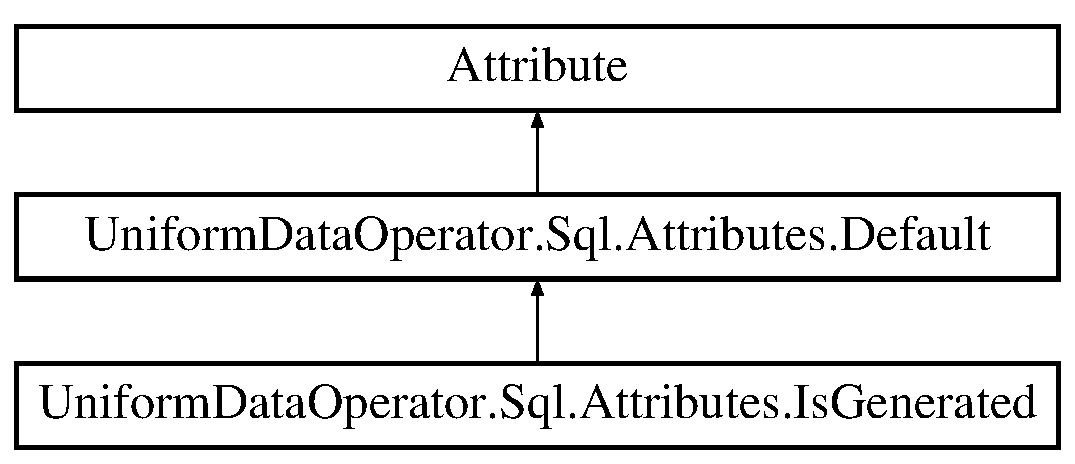
\includegraphics[height=3.000000cm]{d7/daf/class_uniform_data_operator_1_1_sql_1_1_attributes_1_1_is_generated}
\end{center}
\end{figure}
\subsection*{Public Types}
\begin{DoxyCompactItemize}
\item 
enum \mbox{\hyperlink{class_uniform_data_operator_1_1_sql_1_1_attributes_1_1_is_generated_aa8286a355a1ac86ccd56cf5b44f5ed59}{Mode}} \{ \mbox{\hyperlink{class_uniform_data_operator_1_1_sql_1_1_attributes_1_1_is_generated_aa8286a355a1ac86ccd56cf5b44f5ed59a7bf2d26eab899c413218b729d4d914b7}{Mode.\+Stored}}, 
\mbox{\hyperlink{class_uniform_data_operator_1_1_sql_1_1_attributes_1_1_is_generated_aa8286a355a1ac86ccd56cf5b44f5ed59aa6d194ab7efe0417c28a02b8a8997bd0}{Mode.\+Virual}}
 \}
\begin{DoxyCompactList}\small\item\em Modes of generated columns. \end{DoxyCompactList}\end{DoxyCompactItemize}
\subsection*{Public Member Functions}
\begin{DoxyCompactItemize}
\item 
\mbox{\hyperlink{class_uniform_data_operator_1_1_sql_1_1_attributes_1_1_is_generated_ae54943cf65edc20532518f10236ded09}{Is\+Generated}} (\mbox{\hyperlink{class_uniform_data_operator_1_1_sql_1_1_attributes_1_1_is_generated_aa8286a355a1ac86ccd56cf5b44f5ed59}{Mode}} \mbox{\hyperlink{class_uniform_data_operator_1_1_sql_1_1_attributes_1_1_is_generated_a9721250897ee9813cccc2aaa17ec8983}{mode}}, string \mbox{\hyperlink{class_uniform_data_operator_1_1_sql_1_1_attributes_1_1_default_a1ba564b7f35af4395bafa39d6f5f69dc}{def\+Exp}})
\begin{DoxyCompactList}\small\item\em Init generated expression. \end{DoxyCompactList}\end{DoxyCompactItemize}
\subsection*{Public Attributes}
\begin{DoxyCompactItemize}
\item 
\mbox{\hyperlink{class_uniform_data_operator_1_1_sql_1_1_attributes_1_1_is_generated_aa8286a355a1ac86ccd56cf5b44f5ed59}{Mode}} \mbox{\hyperlink{class_uniform_data_operator_1_1_sql_1_1_attributes_1_1_is_generated_a9721250897ee9813cccc2aaa17ec8983}{mode}} = \mbox{\hyperlink{class_uniform_data_operator_1_1_sql_1_1_attributes_1_1_is_generated_aa8286a355a1ac86ccd56cf5b44f5ed59aa6d194ab7efe0417c28a02b8a8997bd0}{Mode.\+Virual}}
\begin{DoxyCompactList}\small\item\em How to operate with value. \end{DoxyCompactList}\end{DoxyCompactItemize}


\subsection{Detailed Description}
Mark field as generated. 



\subsection{Member Enumeration Documentation}
\mbox{\Hypertarget{class_uniform_data_operator_1_1_sql_1_1_attributes_1_1_is_generated_aa8286a355a1ac86ccd56cf5b44f5ed59}\label{class_uniform_data_operator_1_1_sql_1_1_attributes_1_1_is_generated_aa8286a355a1ac86ccd56cf5b44f5ed59}} 
\index{Uniform\+Data\+Operator\+::\+Sql\+::\+Attributes\+::\+Is\+Generated@{Uniform\+Data\+Operator\+::\+Sql\+::\+Attributes\+::\+Is\+Generated}!Mode@{Mode}}
\index{Mode@{Mode}!Uniform\+Data\+Operator\+::\+Sql\+::\+Attributes\+::\+Is\+Generated@{Uniform\+Data\+Operator\+::\+Sql\+::\+Attributes\+::\+Is\+Generated}}
\subsubsection{\texorpdfstring{Mode}{Mode}}
{\footnotesize\ttfamily enum \mbox{\hyperlink{class_uniform_data_operator_1_1_sql_1_1_attributes_1_1_is_generated_aa8286a355a1ac86ccd56cf5b44f5ed59}{Uniform\+Data\+Operator.\+Sql.\+Attributes.\+Is\+Generated.\+Mode}}\hspace{0.3cm}{\ttfamily [strong]}}



Modes of generated columns. 

\begin{DoxyEnumFields}{Enumerator}
\raisebox{\heightof{T}}[0pt][0pt]{\index{Stored@{Stored}!Uniform\+Data\+Operator\+::\+Sql\+::\+Attributes\+::\+Is\+Generated@{Uniform\+Data\+Operator\+::\+Sql\+::\+Attributes\+::\+Is\+Generated}}\index{Uniform\+Data\+Operator\+::\+Sql\+::\+Attributes\+::\+Is\+Generated@{Uniform\+Data\+Operator\+::\+Sql\+::\+Attributes\+::\+Is\+Generated}!Stored@{Stored}}}\mbox{\Hypertarget{class_uniform_data_operator_1_1_sql_1_1_attributes_1_1_is_generated_aa8286a355a1ac86ccd56cf5b44f5ed59a7bf2d26eab899c413218b729d4d914b7}\label{class_uniform_data_operator_1_1_sql_1_1_attributes_1_1_is_generated_aa8286a355a1ac86ccd56cf5b44f5ed59a7bf2d26eab899c413218b729d4d914b7}} 
Stored&Value computed be expression and stored in data base as value. \\
\hline

\raisebox{\heightof{T}}[0pt][0pt]{\index{Virual@{Virual}!Uniform\+Data\+Operator\+::\+Sql\+::\+Attributes\+::\+Is\+Generated@{Uniform\+Data\+Operator\+::\+Sql\+::\+Attributes\+::\+Is\+Generated}}\index{Uniform\+Data\+Operator\+::\+Sql\+::\+Attributes\+::\+Is\+Generated@{Uniform\+Data\+Operator\+::\+Sql\+::\+Attributes\+::\+Is\+Generated}!Virual@{Virual}}}\mbox{\Hypertarget{class_uniform_data_operator_1_1_sql_1_1_attributes_1_1_is_generated_aa8286a355a1ac86ccd56cf5b44f5ed59aa6d194ab7efe0417c28a02b8a8997bd0}\label{class_uniform_data_operator_1_1_sql_1_1_attributes_1_1_is_generated_aa8286a355a1ac86ccd56cf5b44f5ed59aa6d194ab7efe0417c28a02b8a8997bd0}} 
Virual&Value would be computed as expression during every call. \\
\hline

\end{DoxyEnumFields}


\subsection{Constructor \& Destructor Documentation}
\mbox{\Hypertarget{class_uniform_data_operator_1_1_sql_1_1_attributes_1_1_is_generated_ae54943cf65edc20532518f10236ded09}\label{class_uniform_data_operator_1_1_sql_1_1_attributes_1_1_is_generated_ae54943cf65edc20532518f10236ded09}} 
\index{Uniform\+Data\+Operator\+::\+Sql\+::\+Attributes\+::\+Is\+Generated@{Uniform\+Data\+Operator\+::\+Sql\+::\+Attributes\+::\+Is\+Generated}!Is\+Generated@{Is\+Generated}}
\index{Is\+Generated@{Is\+Generated}!Uniform\+Data\+Operator\+::\+Sql\+::\+Attributes\+::\+Is\+Generated@{Uniform\+Data\+Operator\+::\+Sql\+::\+Attributes\+::\+Is\+Generated}}
\subsubsection{\texorpdfstring{Is\+Generated()}{IsGenerated()}}
{\footnotesize\ttfamily Uniform\+Data\+Operator.\+Sql.\+Attributes.\+Is\+Generated.\+Is\+Generated (\begin{DoxyParamCaption}\item[{\mbox{\hyperlink{class_uniform_data_operator_1_1_sql_1_1_attributes_1_1_is_generated_aa8286a355a1ac86ccd56cf5b44f5ed59}{Mode}}}]{mode,  }\item[{string}]{def\+Exp }\end{DoxyParamCaption})}



Init generated expression. 


\begin{DoxyParams}{Parameters}
{\em mode} & How to operate with value.\\
\hline
{\em def\+Exp} & \mbox{\hyperlink{class_uniform_data_operator_1_1_sql_1_1_attributes_1_1_default}{Default}} or Expression value.\\
\hline
\end{DoxyParams}


\subsection{Member Data Documentation}
\mbox{\Hypertarget{class_uniform_data_operator_1_1_sql_1_1_attributes_1_1_is_generated_a9721250897ee9813cccc2aaa17ec8983}\label{class_uniform_data_operator_1_1_sql_1_1_attributes_1_1_is_generated_a9721250897ee9813cccc2aaa17ec8983}} 
\index{Uniform\+Data\+Operator\+::\+Sql\+::\+Attributes\+::\+Is\+Generated@{Uniform\+Data\+Operator\+::\+Sql\+::\+Attributes\+::\+Is\+Generated}!mode@{mode}}
\index{mode@{mode}!Uniform\+Data\+Operator\+::\+Sql\+::\+Attributes\+::\+Is\+Generated@{Uniform\+Data\+Operator\+::\+Sql\+::\+Attributes\+::\+Is\+Generated}}
\subsubsection{\texorpdfstring{mode}{mode}}
{\footnotesize\ttfamily \mbox{\hyperlink{class_uniform_data_operator_1_1_sql_1_1_attributes_1_1_is_generated_aa8286a355a1ac86ccd56cf5b44f5ed59}{Mode}} Uniform\+Data\+Operator.\+Sql.\+Attributes.\+Is\+Generated.\+mode = \mbox{\hyperlink{class_uniform_data_operator_1_1_sql_1_1_attributes_1_1_is_generated_aa8286a355a1ac86ccd56cf5b44f5ed59aa6d194ab7efe0417c28a02b8a8997bd0}{Mode.\+Virual}}}



How to operate with value. 



The documentation for this class was generated from the following file\+:\begin{DoxyCompactItemize}
\item 
D\+:/\+Work/\+Git\+Hub/uniform-\/data-\/operator/\+S\+Q\+L/\+Attributes/Is\+Generated.\+cs\end{DoxyCompactItemize}

\hypertarget{class_uniform_data_operator_1_1_sql_1_1_attributes_1_1_is_not_null}{}\section{Uniform\+Data\+Operator.\+Sql.\+Attributes.\+Is\+Not\+Null Class Reference}
\label{class_uniform_data_operator_1_1_sql_1_1_attributes_1_1_is_not_null}\index{Uniform\+Data\+Operator.\+Sql.\+Attributes.\+Is\+Not\+Null@{Uniform\+Data\+Operator.\+Sql.\+Attributes.\+Is\+Not\+Null}}


Is value always not null.  


Inheritance diagram for Uniform\+Data\+Operator.\+Sql.\+Attributes.\+Is\+Not\+Null\+:\begin{figure}[H]
\begin{center}
\leavevmode
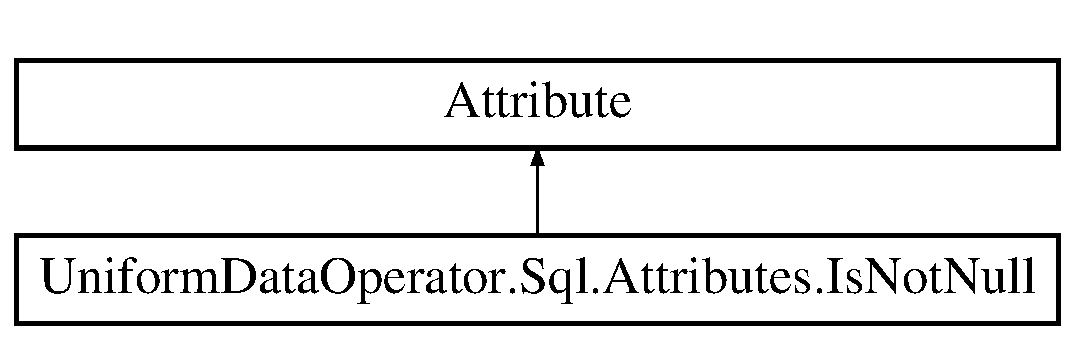
\includegraphics[height=2.000000cm]{d4/d02/class_uniform_data_operator_1_1_sql_1_1_attributes_1_1_is_not_null}
\end{center}
\end{figure}


\subsection{Detailed Description}
Is value always not null. 



The documentation for this class was generated from the following file\+:\begin{DoxyCompactItemize}
\item 
D\+:/\+Work/\+Git\+Hub/uniform-\/data-\/operator/\+S\+Q\+L/\+Attributes/Is\+Not\+Null.\+cs\end{DoxyCompactItemize}

\hypertarget{class_uniform_data_operator_1_1_sql_1_1_attributes_1_1_is_primary_key}{}\section{Uniform\+Data\+Operator.\+Sql.\+Attributes.\+Is\+Primary\+Key Class Reference}
\label{class_uniform_data_operator_1_1_sql_1_1_attributes_1_1_is_primary_key}\index{Uniform\+Data\+Operator.\+Sql.\+Attributes.\+Is\+Primary\+Key@{Uniform\+Data\+Operator.\+Sql.\+Attributes.\+Is\+Primary\+Key}}


Is it\textquotesingle{}s primary key.  


Inheritance diagram for Uniform\+Data\+Operator.\+Sql.\+Attributes.\+Is\+Primary\+Key\+:\begin{figure}[H]
\begin{center}
\leavevmode
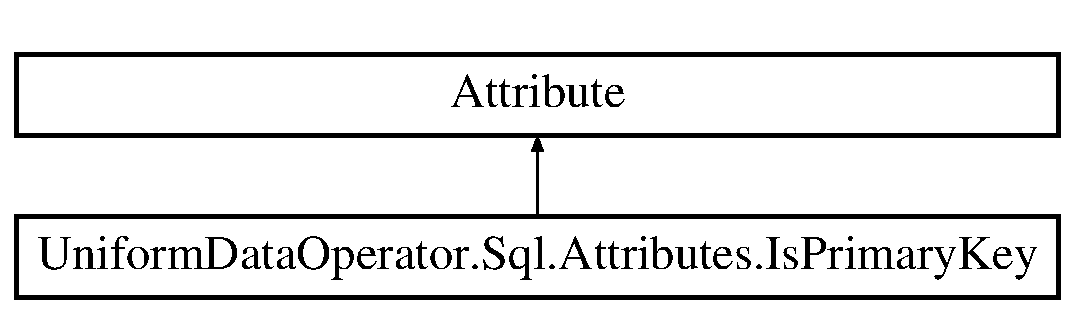
\includegraphics[height=2.000000cm]{d4/da1/class_uniform_data_operator_1_1_sql_1_1_attributes_1_1_is_primary_key}
\end{center}
\end{figure}


\subsection{Detailed Description}
Is it\textquotesingle{}s primary key. 



The documentation for this class was generated from the following file\+:\begin{DoxyCompactItemize}
\item 
D\+:/\+Work/\+Git\+Hub/uniform-\/data-\/operator/\+S\+Q\+L/\+Attributes/Is\+Primary\+Key.\+cs\end{DoxyCompactItemize}

\hypertarget{interface_uniform_data_operator_1_1_sql_1_1_i_sql_operator}{}\section{Uniform\+Data\+Operator.\+Sql.\+I\+Sql\+Operator Interface Reference}
\label{interface_uniform_data_operator_1_1_sql_1_1_i_sql_operator}\index{Uniform\+Data\+Operator.\+Sql.\+I\+Sql\+Operator@{Uniform\+Data\+Operator.\+Sql.\+I\+Sql\+Operator}}


Implement that interface to provide possiblity to controll your data base by using S\+QL queryes.  


Inheritance diagram for Uniform\+Data\+Operator.\+Sql.\+I\+Sql\+Operator\+:\begin{figure}[H]
\begin{center}
\leavevmode
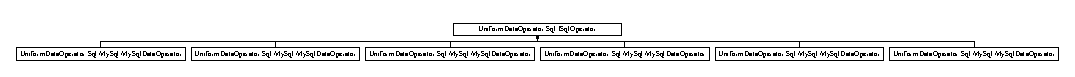
\includegraphics[height=0.590717cm]{d1/dad/interface_uniform_data_operator_1_1_sql_1_1_i_sql_operator}
\end{center}
\end{figure}
\subsection*{Public Member Functions}
\begin{DoxyCompactItemize}
\item 
void \mbox{\hyperlink{interface_uniform_data_operator_1_1_sql_1_1_i_sql_operator_a590fa080f8c35ebf5ee6ac535545e2a8}{Initialize}} ()
\begin{DoxyCompactList}\small\item\em Initialize operator. \end{DoxyCompactList}\item 
Db\+Command \mbox{\hyperlink{interface_uniform_data_operator_1_1_sql_1_1_i_sql_operator_afc0fd8b8c82515c498a6959453f331f1}{New\+Command}} ()
\begin{DoxyCompactList}\small\item\em Return new clear command suitable for current DB. \end{DoxyCompactList}\item 
Db\+Command \mbox{\hyperlink{interface_uniform_data_operator_1_1_sql_1_1_i_sql_operator_a10c43a3bfb6e8c88b692488c3341f297}{New\+Command}} (string command\+Text)
\begin{DoxyCompactList}\small\item\em Return new clear command suitable for current DB with included command text. \end{DoxyCompactList}\item 
Db\+Parameter \mbox{\hyperlink{interface_uniform_data_operator_1_1_sql_1_1_i_sql_operator_ab43375e7f5d9dcce2adfef2f19a2078f}{Member\+To\+Parameter}} (object data, \mbox{\hyperlink{class_uniform_data_operator_1_1_sql_1_1_tables_1_1_attributes_1_1_column}{Tables.\+Attributes.\+Column}} column)
\begin{DoxyCompactList}\small\item\em Convert value of member to data base parameter that can be used in command. \end{DoxyCompactList}\item 
Db\+Command \mbox{\hyperlink{interface_uniform_data_operator_1_1_sql_1_1_i_sql_operator_a12d464e0532a3e194b1221eee0c32d34}{Disable\+Sql\+Checks}} (Db\+Command command)
\begin{DoxyCompactList}\small\item\em Add code that disabling S\+QL checks during executing command. \end{DoxyCompactList}\item 
string \mbox{\hyperlink{interface_uniform_data_operator_1_1_sql_1_1_i_sql_operator_a0757f304a24ffaa743e23e8bdd210950}{Disable\+Sql\+Checks}} (string command)
\begin{DoxyCompactList}\small\item\em Add code that disabling S\+QL checks during executing command. \end{DoxyCompactList}\item 
string \mbox{\hyperlink{interface_uniform_data_operator_1_1_sql_1_1_i_sql_operator_a51af40df39808d53cdcc81852b836634}{Db\+Type\+To\+String}} (Db\+Type type)
\begin{DoxyCompactList}\small\item\em Trying to convert D\+B\+Type to specified type in string format that suitable to this database. \end{DoxyCompactList}\item 
bool \mbox{\hyperlink{interface_uniform_data_operator_1_1_sql_1_1_i_sql_operator_a3b5fbe97e664e1ef689576ab8757f957}{Validate\+Table\+Member}} (\mbox{\hyperlink{class_uniform_data_operator_1_1_sql_1_1_tables_1_1_attributes_1_1_table}{Table}} table\+Descriptor, Member\+Info column\+Member)
\begin{DoxyCompactList}\small\item\em Validate data base table column acording to member attributes. \end{DoxyCompactList}\item 
bool \mbox{\hyperlink{interface_uniform_data_operator_1_1_sql_1_1_i_sql_operator_a6fc9e5efd1e21ae9998b9c56ae9e347c}{Open\+Connection}} (out string error)
\begin{DoxyCompactList}\small\item\em Opening connection to S\+QL server. \end{DoxyCompactList}\item 
bool \mbox{\hyperlink{interface_uniform_data_operator_1_1_sql_1_1_i_sql_operator_a1a6429996e1bbb452f4e034fd634e640}{Close\+Connection}} ()
\begin{DoxyCompactList}\small\item\em Closing connection to S\+QL server. \end{DoxyCompactList}\item 
void \mbox{\hyperlink{interface_uniform_data_operator_1_1_sql_1_1_i_sql_operator_a096be4f746c1fcbb8b2894c2517b937c}{Backup}} (string directory)
\begin{DoxyCompactList}\small\item\em Backuping data base to sql file in directory. Name would be generated by timestamp. \end{DoxyCompactList}\item 
void \mbox{\hyperlink{interface_uniform_data_operator_1_1_sql_1_1_i_sql_operator_acf6fdbfc57a21efc371e0772244defd5}{Restore}} (string file\+Path)
\begin{DoxyCompactList}\small\item\em Restoring S\+QL db from file. \end{DoxyCompactList}\item 
bool \mbox{\hyperlink{interface_uniform_data_operator_1_1_sql_1_1_i_sql_operator_a5ae8328a464ef80f1ae1bd46a573c265}{Activate\+Schema}} (string schema\+Name, out string error)
\begin{DoxyCompactList}\small\item\em Trying to set schema to databases server in case if shema not exist. \end{DoxyCompactList}\item 
string \mbox{\hyperlink{interface_uniform_data_operator_1_1_sql_1_1_i_sql_operator_aac9c3ed1e73af66e383340a154786ec7}{Column\+Declaration\+Command}} (Member\+Info member)
\begin{DoxyCompactList}\small\item\em Return generated S\+QL command relative to init time. \end{DoxyCompactList}\item 
bool \mbox{\hyperlink{interface_uniform_data_operator_1_1_sql_1_1_i_sql_operator_ad05106eb6bd1a50f35b476a42821dfa3}{Set\+To\+Table}} (Type table\+Type, object data, out string error)
\begin{DoxyCompactList}\small\item\em Creating request that setting up data from object to data base server acording to attributes. \end{DoxyCompactList}\item 
Task \mbox{\hyperlink{interface_uniform_data_operator_1_1_sql_1_1_i_sql_operator_a35ef3899954f213e391751e9cda09322}{Set\+To\+Table\+Async}} (Type table\+Type, Cancellation\+Token cancellation\+Token, object data)
\begin{DoxyCompactList}\small\item\em Creating request that setting up data from object to data base server acording to attributes. \end{DoxyCompactList}\item 
bool \mbox{\hyperlink{interface_uniform_data_operator_1_1_sql_1_1_i_sql_operator_a9a1822fcafcb1a3abd59b40f2cef7930}{Set\+To\+Object}} (Type table\+Type, object obj, out string error, string\mbox{[}$\,$\mbox{]} select, params string\mbox{[}$\,$\mbox{]} where)
\begin{DoxyCompactList}\small\item\em Setting data from DB Data reader to object by using column map described at object Type. Auto-\/generate S\+QL query and request coluns data relative to privary keys described in object. \end{DoxyCompactList}\item 
bool \mbox{\hyperlink{interface_uniform_data_operator_1_1_sql_1_1_i_sql_operator_ae1053edf9aa3d9385ef3591e7ee863c7}{Set\+To\+Object}} (Type table\+Type, object obj, out string error, params string\mbox{[}$\,$\mbox{]} selsect)
\begin{DoxyCompactList}\small\item\em Setting data from DB Data reader to object by using column map described at object Type. Auto-\/generate S\+QL query and request coluns data relative to privary keys described in object. \end{DoxyCompactList}\item 
bool \mbox{\hyperlink{interface_uniform_data_operator_1_1_sql_1_1_i_sql_operator_ac170526dd0fa31f2848ece5f5c5bb9d7}{Set\+To\+Object}} (Type table\+Type, object obj, out string error)
\begin{DoxyCompactList}\small\item\em Setting data from DB Data reader to object by using column map described at object Type. Auto-\/generate S\+QL query and request coluns data relative to privary keys described in object. \end{DoxyCompactList}\item 
Task \mbox{\hyperlink{interface_uniform_data_operator_1_1_sql_1_1_i_sql_operator_a16e1513f43f3b9d76c687ba3b026573d}{Set\+To\+Object\+Async}} (Type table\+Type, Cancellation\+Token cancellation\+Token, object obj, string\mbox{[}$\,$\mbox{]} select, params string\mbox{[}$\,$\mbox{]} where)
\begin{DoxyCompactList}\small\item\em Setting data from DB Data reader to object by using column map described at object Type. Auto-\/generate S\+QL query and request coluns data relative to privary keys described in object. \end{DoxyCompactList}\item 
Task \mbox{\hyperlink{interface_uniform_data_operator_1_1_sql_1_1_i_sql_operator_a3a973b49f190dabe6bcd0bf3e79b3c5e}{Set\+To\+Object\+Async}} (Type table\+Type, Cancellation\+Token cancellation\+Token, object obj, params string\mbox{[}$\,$\mbox{]} select)
\begin{DoxyCompactList}\small\item\em Setting data from DB Data reader to object by using column map described at object Type. Auto-\/generate S\+QL query and request coluns data relative to privary keys described in object. \end{DoxyCompactList}\item 
Task \mbox{\hyperlink{interface_uniform_data_operator_1_1_sql_1_1_i_sql_operator_a497325acf359d4f8444ee0c2ff858e6e}{Set\+To\+Object\+Async}} (Type table\+Type, Cancellation\+Token cancellation\+Token, object obj)
\begin{DoxyCompactList}\small\item\em Setting data from DB Data reader to object by using column map described at object Type. Auto-\/generate S\+QL query and request coluns data relative to privary keys described in object. \end{DoxyCompactList}\end{DoxyCompactItemize}
\subsection*{Properties}
\begin{DoxyCompactItemize}
\item 
string \mbox{\hyperlink{interface_uniform_data_operator_1_1_sql_1_1_i_sql_operator_ab1b593e38cb9377dac847811c483f2f3}{Server}}\hspace{0.3cm}{\ttfamily  \mbox{[}get, set\mbox{]}}
\begin{DoxyCompactList}\small\item\em Server\textquotesingle{}s ip. \end{DoxyCompactList}\item 
int \mbox{\hyperlink{interface_uniform_data_operator_1_1_sql_1_1_i_sql_operator_a2d0ac2538fa196b181f6e0ab523db137}{Port}}\hspace{0.3cm}{\ttfamily  \mbox{[}get, set\mbox{]}}
\begin{DoxyCompactList}\small\item\em Port for server access. \end{DoxyCompactList}\item 
string \mbox{\hyperlink{interface_uniform_data_operator_1_1_sql_1_1_i_sql_operator_a55b7f28ed4ab20f124e67e2d447f8b40}{Database}}\hspace{0.3cm}{\ttfamily  \mbox{[}get, set\mbox{]}}
\begin{DoxyCompactList}\small\item\em Database\textquotesingle{}s name. \end{DoxyCompactList}\item 
string \mbox{\hyperlink{interface_uniform_data_operator_1_1_sql_1_1_i_sql_operator_abf0c3a32c8161030b37ccf960c395d4f}{User\+Id}}\hspace{0.3cm}{\ttfamily  \mbox{[}get, set\mbox{]}}
\begin{DoxyCompactList}\small\item\em User for connection. \end{DoxyCompactList}\item 
string \mbox{\hyperlink{interface_uniform_data_operator_1_1_sql_1_1_i_sql_operator_a90f63ab37347ec080b37dc3256ead7a4}{Password}}\hspace{0.3cm}{\ttfamily  \mbox{[}get, set\mbox{]}}
\begin{DoxyCompactList}\small\item\em User\textquotesingle{}s password. \end{DoxyCompactList}\item 
Db\+Connection \mbox{\hyperlink{interface_uniform_data_operator_1_1_sql_1_1_i_sql_operator_a99f034a986828e96955e3187cdfb28da}{Connection}}\hspace{0.3cm}{\ttfamily  \mbox{[}get\mbox{]}}
\begin{DoxyCompactList}\small\item\em Connection to DB. \end{DoxyCompactList}\end{DoxyCompactItemize}


\subsection{Detailed Description}
Implement that interface to provide possiblity to controll your data base by using S\+QL queryes. 



\subsection{Member Function Documentation}
\mbox{\Hypertarget{interface_uniform_data_operator_1_1_sql_1_1_i_sql_operator_a5ae8328a464ef80f1ae1bd46a573c265}\label{interface_uniform_data_operator_1_1_sql_1_1_i_sql_operator_a5ae8328a464ef80f1ae1bd46a573c265}} 
\index{Uniform\+Data\+Operator\+::\+Sql\+::\+I\+Sql\+Operator@{Uniform\+Data\+Operator\+::\+Sql\+::\+I\+Sql\+Operator}!Activate\+Schema@{Activate\+Schema}}
\index{Activate\+Schema@{Activate\+Schema}!Uniform\+Data\+Operator\+::\+Sql\+::\+I\+Sql\+Operator@{Uniform\+Data\+Operator\+::\+Sql\+::\+I\+Sql\+Operator}}
\subsubsection{\texorpdfstring{Activate\+Schema()}{ActivateSchema()}}
{\footnotesize\ttfamily bool Uniform\+Data\+Operator.\+Sql.\+I\+Sql\+Operator.\+Activate\+Schema (\begin{DoxyParamCaption}\item[{string}]{schema\+Name,  }\item[{out string}]{error }\end{DoxyParamCaption})}



Trying to set schema to databases server in case if shema not exist. 


\begin{DoxyParams}{Parameters}
{\em schema\+Name} & Name of the schema that would be used.\\
\hline
{\em error} & Error faces during operation.\\
\hline
\end{DoxyParams}
\begin{DoxyReturn}{Returns}

\end{DoxyReturn}


Implemented in \mbox{\hyperlink{class_uniform_data_operator_1_1_sql_1_1_my_sql_1_1_my_sql_data_operator_a2ed7d06bc016ae6d07cbcceffc21bbd3}{Uniform\+Data\+Operator.\+Sql.\+My\+Sql.\+My\+Sql\+Data\+Operator}}.

\mbox{\Hypertarget{interface_uniform_data_operator_1_1_sql_1_1_i_sql_operator_a096be4f746c1fcbb8b2894c2517b937c}\label{interface_uniform_data_operator_1_1_sql_1_1_i_sql_operator_a096be4f746c1fcbb8b2894c2517b937c}} 
\index{Uniform\+Data\+Operator\+::\+Sql\+::\+I\+Sql\+Operator@{Uniform\+Data\+Operator\+::\+Sql\+::\+I\+Sql\+Operator}!Backup@{Backup}}
\index{Backup@{Backup}!Uniform\+Data\+Operator\+::\+Sql\+::\+I\+Sql\+Operator@{Uniform\+Data\+Operator\+::\+Sql\+::\+I\+Sql\+Operator}}
\subsubsection{\texorpdfstring{Backup()}{Backup()}}
{\footnotesize\ttfamily void Uniform\+Data\+Operator.\+Sql.\+I\+Sql\+Operator.\+Backup (\begin{DoxyParamCaption}\item[{string}]{directory }\end{DoxyParamCaption})}



Backuping data base to sql file in directory. Name would be generated by timestamp. 


\begin{DoxyParams}{Parameters}
{\em directory} & Directory that would store the backup file.\\
\hline
\end{DoxyParams}


Implemented in \mbox{\hyperlink{class_uniform_data_operator_1_1_sql_1_1_my_sql_1_1_my_sql_data_operator_a0dbd58206733a17dd26143b58d0859d7}{Uniform\+Data\+Operator.\+Sql.\+My\+Sql.\+My\+Sql\+Data\+Operator}}.

\mbox{\Hypertarget{interface_uniform_data_operator_1_1_sql_1_1_i_sql_operator_a1a6429996e1bbb452f4e034fd634e640}\label{interface_uniform_data_operator_1_1_sql_1_1_i_sql_operator_a1a6429996e1bbb452f4e034fd634e640}} 
\index{Uniform\+Data\+Operator\+::\+Sql\+::\+I\+Sql\+Operator@{Uniform\+Data\+Operator\+::\+Sql\+::\+I\+Sql\+Operator}!Close\+Connection@{Close\+Connection}}
\index{Close\+Connection@{Close\+Connection}!Uniform\+Data\+Operator\+::\+Sql\+::\+I\+Sql\+Operator@{Uniform\+Data\+Operator\+::\+Sql\+::\+I\+Sql\+Operator}}
\subsubsection{\texorpdfstring{Close\+Connection()}{CloseConnection()}}
{\footnotesize\ttfamily bool Uniform\+Data\+Operator.\+Sql.\+I\+Sql\+Operator.\+Close\+Connection (\begin{DoxyParamCaption}{ }\end{DoxyParamCaption})}



Closing connection to S\+QL server. 

\begin{DoxyReturn}{Returns}
Result of connection closing.
\end{DoxyReturn}


Implemented in \mbox{\hyperlink{class_uniform_data_operator_1_1_sql_1_1_my_sql_1_1_my_sql_data_operator_ae096306ef55611afbe96b0017f2032f6}{Uniform\+Data\+Operator.\+Sql.\+My\+Sql.\+My\+Sql\+Data\+Operator}}.

\mbox{\Hypertarget{interface_uniform_data_operator_1_1_sql_1_1_i_sql_operator_aac9c3ed1e73af66e383340a154786ec7}\label{interface_uniform_data_operator_1_1_sql_1_1_i_sql_operator_aac9c3ed1e73af66e383340a154786ec7}} 
\index{Uniform\+Data\+Operator\+::\+Sql\+::\+I\+Sql\+Operator@{Uniform\+Data\+Operator\+::\+Sql\+::\+I\+Sql\+Operator}!Column\+Declaration\+Command@{Column\+Declaration\+Command}}
\index{Column\+Declaration\+Command@{Column\+Declaration\+Command}!Uniform\+Data\+Operator\+::\+Sql\+::\+I\+Sql\+Operator@{Uniform\+Data\+Operator\+::\+Sql\+::\+I\+Sql\+Operator}}
\subsubsection{\texorpdfstring{Column\+Declaration\+Command()}{ColumnDeclarationCommand()}}
{\footnotesize\ttfamily string Uniform\+Data\+Operator.\+Sql.\+I\+Sql\+Operator.\+Column\+Declaration\+Command (\begin{DoxyParamCaption}\item[{Member\+Info}]{member }\end{DoxyParamCaption})}



Return generated S\+QL command relative to init time. 


\begin{DoxyParams}{Parameters}
{\em member} & Member that contains defined attributes that describes column definition.\\
\hline
\end{DoxyParams}
\begin{DoxyReturn}{Returns}
S\+QL command relative to target server.
\end{DoxyReturn}


Implemented in \mbox{\hyperlink{class_uniform_data_operator_1_1_sql_1_1_my_sql_1_1_my_sql_data_operator_a0bdc2943e5d10576fb564913cdd744e7}{Uniform\+Data\+Operator.\+Sql.\+My\+Sql.\+My\+Sql\+Data\+Operator}}.

\mbox{\Hypertarget{interface_uniform_data_operator_1_1_sql_1_1_i_sql_operator_a51af40df39808d53cdcc81852b836634}\label{interface_uniform_data_operator_1_1_sql_1_1_i_sql_operator_a51af40df39808d53cdcc81852b836634}} 
\index{Uniform\+Data\+Operator\+::\+Sql\+::\+I\+Sql\+Operator@{Uniform\+Data\+Operator\+::\+Sql\+::\+I\+Sql\+Operator}!Db\+Type\+To\+String@{Db\+Type\+To\+String}}
\index{Db\+Type\+To\+String@{Db\+Type\+To\+String}!Uniform\+Data\+Operator\+::\+Sql\+::\+I\+Sql\+Operator@{Uniform\+Data\+Operator\+::\+Sql\+::\+I\+Sql\+Operator}}
\subsubsection{\texorpdfstring{Db\+Type\+To\+String()}{DbTypeToString()}}
{\footnotesize\ttfamily string Uniform\+Data\+Operator.\+Sql.\+I\+Sql\+Operator.\+Db\+Type\+To\+String (\begin{DoxyParamCaption}\item[{Db\+Type}]{type }\end{DoxyParamCaption})}



Trying to convert D\+B\+Type to specified type in string format that suitable to this database. 


\begin{DoxyParams}{Parameters}
{\em type} & Common D\+B\+Type.\\
\hline
\end{DoxyParams}
\begin{DoxyReturn}{Returns}
Type suitable for S\+QL command relative to this type of data base. Invalid\+Cast\+Exception in case if converting not possible.
\end{DoxyReturn}


Implemented in \mbox{\hyperlink{class_uniform_data_operator_1_1_sql_1_1_my_sql_1_1_my_sql_data_operator_a7b854ebbcdf31c67716d8c365c321a31}{Uniform\+Data\+Operator.\+Sql.\+My\+Sql.\+My\+Sql\+Data\+Operator}}.

\mbox{\Hypertarget{interface_uniform_data_operator_1_1_sql_1_1_i_sql_operator_a12d464e0532a3e194b1221eee0c32d34}\label{interface_uniform_data_operator_1_1_sql_1_1_i_sql_operator_a12d464e0532a3e194b1221eee0c32d34}} 
\index{Uniform\+Data\+Operator\+::\+Sql\+::\+I\+Sql\+Operator@{Uniform\+Data\+Operator\+::\+Sql\+::\+I\+Sql\+Operator}!Disable\+Sql\+Checks@{Disable\+Sql\+Checks}}
\index{Disable\+Sql\+Checks@{Disable\+Sql\+Checks}!Uniform\+Data\+Operator\+::\+Sql\+::\+I\+Sql\+Operator@{Uniform\+Data\+Operator\+::\+Sql\+::\+I\+Sql\+Operator}}
\subsubsection{\texorpdfstring{Disable\+Sql\+Checks()}{DisableSqlChecks()}\hspace{0.1cm}{\footnotesize\ttfamily [1/2]}}
{\footnotesize\ttfamily Db\+Command Uniform\+Data\+Operator.\+Sql.\+I\+Sql\+Operator.\+Disable\+Sql\+Checks (\begin{DoxyParamCaption}\item[{Db\+Command}]{command }\end{DoxyParamCaption})}



Add code that disabling S\+QL checks during executing command. 


\begin{DoxyParams}{Parameters}
{\em command} & Target command that would be modified during operation.\\
\hline
\end{DoxyParams}
\begin{DoxyReturn}{Returns}
Modified comand.
\end{DoxyReturn}


Implemented in \mbox{\hyperlink{class_uniform_data_operator_1_1_sql_1_1_my_sql_1_1_my_sql_data_operator_affbacb4fb1773fc14cdbb9cbcd315c5f}{Uniform\+Data\+Operator.\+Sql.\+My\+Sql.\+My\+Sql\+Data\+Operator}}.

\mbox{\Hypertarget{interface_uniform_data_operator_1_1_sql_1_1_i_sql_operator_a0757f304a24ffaa743e23e8bdd210950}\label{interface_uniform_data_operator_1_1_sql_1_1_i_sql_operator_a0757f304a24ffaa743e23e8bdd210950}} 
\index{Uniform\+Data\+Operator\+::\+Sql\+::\+I\+Sql\+Operator@{Uniform\+Data\+Operator\+::\+Sql\+::\+I\+Sql\+Operator}!Disable\+Sql\+Checks@{Disable\+Sql\+Checks}}
\index{Disable\+Sql\+Checks@{Disable\+Sql\+Checks}!Uniform\+Data\+Operator\+::\+Sql\+::\+I\+Sql\+Operator@{Uniform\+Data\+Operator\+::\+Sql\+::\+I\+Sql\+Operator}}
\subsubsection{\texorpdfstring{Disable\+Sql\+Checks()}{DisableSqlChecks()}\hspace{0.1cm}{\footnotesize\ttfamily [2/2]}}
{\footnotesize\ttfamily string Uniform\+Data\+Operator.\+Sql.\+I\+Sql\+Operator.\+Disable\+Sql\+Checks (\begin{DoxyParamCaption}\item[{string}]{command }\end{DoxyParamCaption})}



Add code that disabling S\+QL checks during executing command. 


\begin{DoxyParams}{Parameters}
{\em command} & Target command that would be modified during operation.\\
\hline
\end{DoxyParams}
\begin{DoxyReturn}{Returns}
Modified comand.
\end{DoxyReturn}


Implemented in \mbox{\hyperlink{class_uniform_data_operator_1_1_sql_1_1_my_sql_1_1_my_sql_data_operator_a3e80f9136c9fef46a443901a15f1e289}{Uniform\+Data\+Operator.\+Sql.\+My\+Sql.\+My\+Sql\+Data\+Operator}}.

\mbox{\Hypertarget{interface_uniform_data_operator_1_1_sql_1_1_i_sql_operator_a590fa080f8c35ebf5ee6ac535545e2a8}\label{interface_uniform_data_operator_1_1_sql_1_1_i_sql_operator_a590fa080f8c35ebf5ee6ac535545e2a8}} 
\index{Uniform\+Data\+Operator\+::\+Sql\+::\+I\+Sql\+Operator@{Uniform\+Data\+Operator\+::\+Sql\+::\+I\+Sql\+Operator}!Initialize@{Initialize}}
\index{Initialize@{Initialize}!Uniform\+Data\+Operator\+::\+Sql\+::\+I\+Sql\+Operator@{Uniform\+Data\+Operator\+::\+Sql\+::\+I\+Sql\+Operator}}
\subsubsection{\texorpdfstring{Initialize()}{Initialize()}}
{\footnotesize\ttfamily void Uniform\+Data\+Operator.\+Sql.\+I\+Sql\+Operator.\+Initialize (\begin{DoxyParamCaption}{ }\end{DoxyParamCaption})}



Initialize operator. 



Implemented in \mbox{\hyperlink{class_uniform_data_operator_1_1_sql_1_1_my_sql_1_1_my_sql_data_operator_a5aad834d2ceba598037b6ed19b27db6d}{Uniform\+Data\+Operator.\+Sql.\+My\+Sql.\+My\+Sql\+Data\+Operator}}.

\mbox{\Hypertarget{interface_uniform_data_operator_1_1_sql_1_1_i_sql_operator_ab43375e7f5d9dcce2adfef2f19a2078f}\label{interface_uniform_data_operator_1_1_sql_1_1_i_sql_operator_ab43375e7f5d9dcce2adfef2f19a2078f}} 
\index{Uniform\+Data\+Operator\+::\+Sql\+::\+I\+Sql\+Operator@{Uniform\+Data\+Operator\+::\+Sql\+::\+I\+Sql\+Operator}!Member\+To\+Parameter@{Member\+To\+Parameter}}
\index{Member\+To\+Parameter@{Member\+To\+Parameter}!Uniform\+Data\+Operator\+::\+Sql\+::\+I\+Sql\+Operator@{Uniform\+Data\+Operator\+::\+Sql\+::\+I\+Sql\+Operator}}
\subsubsection{\texorpdfstring{Member\+To\+Parameter()}{MemberToParameter()}}
{\footnotesize\ttfamily Db\+Parameter Uniform\+Data\+Operator.\+Sql.\+I\+Sql\+Operator.\+Member\+To\+Parameter (\begin{DoxyParamCaption}\item[{object}]{data,  }\item[{\mbox{\hyperlink{class_uniform_data_operator_1_1_sql_1_1_tables_1_1_attributes_1_1_column}{Tables.\+Attributes.\+Column}}}]{column }\end{DoxyParamCaption})}



Convert value of member to data base parameter that can be used in command. 


\begin{DoxyParams}{Parameters}
{\em data} & Value of the object that would applied to parameter.\\
\hline
{\em column} & Column attribute relative to member of data.\\
\hline
\end{DoxyParams}
\begin{DoxyReturn}{Returns}
Parameter that could by used in commands to data base.
\end{DoxyReturn}
\mbox{\Hypertarget{interface_uniform_data_operator_1_1_sql_1_1_i_sql_operator_afc0fd8b8c82515c498a6959453f331f1}\label{interface_uniform_data_operator_1_1_sql_1_1_i_sql_operator_afc0fd8b8c82515c498a6959453f331f1}} 
\index{Uniform\+Data\+Operator\+::\+Sql\+::\+I\+Sql\+Operator@{Uniform\+Data\+Operator\+::\+Sql\+::\+I\+Sql\+Operator}!New\+Command@{New\+Command}}
\index{New\+Command@{New\+Command}!Uniform\+Data\+Operator\+::\+Sql\+::\+I\+Sql\+Operator@{Uniform\+Data\+Operator\+::\+Sql\+::\+I\+Sql\+Operator}}
\subsubsection{\texorpdfstring{New\+Command()}{NewCommand()}\hspace{0.1cm}{\footnotesize\ttfamily [1/2]}}
{\footnotesize\ttfamily Db\+Command Uniform\+Data\+Operator.\+Sql.\+I\+Sql\+Operator.\+New\+Command (\begin{DoxyParamCaption}{ }\end{DoxyParamCaption})}



Return new clear command suitable for current DB. 



Implemented in \mbox{\hyperlink{class_uniform_data_operator_1_1_sql_1_1_my_sql_1_1_my_sql_data_operator_af5850bfb38f7dfcd5acd5157458ef4bd}{Uniform\+Data\+Operator.\+Sql.\+My\+Sql.\+My\+Sql\+Data\+Operator}}.

\mbox{\Hypertarget{interface_uniform_data_operator_1_1_sql_1_1_i_sql_operator_a10c43a3bfb6e8c88b692488c3341f297}\label{interface_uniform_data_operator_1_1_sql_1_1_i_sql_operator_a10c43a3bfb6e8c88b692488c3341f297}} 
\index{Uniform\+Data\+Operator\+::\+Sql\+::\+I\+Sql\+Operator@{Uniform\+Data\+Operator\+::\+Sql\+::\+I\+Sql\+Operator}!New\+Command@{New\+Command}}
\index{New\+Command@{New\+Command}!Uniform\+Data\+Operator\+::\+Sql\+::\+I\+Sql\+Operator@{Uniform\+Data\+Operator\+::\+Sql\+::\+I\+Sql\+Operator}}
\subsubsection{\texorpdfstring{New\+Command()}{NewCommand()}\hspace{0.1cm}{\footnotesize\ttfamily [2/2]}}
{\footnotesize\ttfamily Db\+Command Uniform\+Data\+Operator.\+Sql.\+I\+Sql\+Operator.\+New\+Command (\begin{DoxyParamCaption}\item[{string}]{command\+Text }\end{DoxyParamCaption})}



Return new clear command suitable for current DB with included command text. 



Implemented in \mbox{\hyperlink{class_uniform_data_operator_1_1_sql_1_1_my_sql_1_1_my_sql_data_operator_a6c2e2d374072c275953a515379963881}{Uniform\+Data\+Operator.\+Sql.\+My\+Sql.\+My\+Sql\+Data\+Operator}}.

\mbox{\Hypertarget{interface_uniform_data_operator_1_1_sql_1_1_i_sql_operator_a6fc9e5efd1e21ae9998b9c56ae9e347c}\label{interface_uniform_data_operator_1_1_sql_1_1_i_sql_operator_a6fc9e5efd1e21ae9998b9c56ae9e347c}} 
\index{Uniform\+Data\+Operator\+::\+Sql\+::\+I\+Sql\+Operator@{Uniform\+Data\+Operator\+::\+Sql\+::\+I\+Sql\+Operator}!Open\+Connection@{Open\+Connection}}
\index{Open\+Connection@{Open\+Connection}!Uniform\+Data\+Operator\+::\+Sql\+::\+I\+Sql\+Operator@{Uniform\+Data\+Operator\+::\+Sql\+::\+I\+Sql\+Operator}}
\subsubsection{\texorpdfstring{Open\+Connection()}{OpenConnection()}}
{\footnotesize\ttfamily bool Uniform\+Data\+Operator.\+Sql.\+I\+Sql\+Operator.\+Open\+Connection (\begin{DoxyParamCaption}\item[{out string}]{error }\end{DoxyParamCaption})}



Opening connection to S\+QL server. 


\begin{DoxyParams}{Parameters}
{\em error} & Faced error. Null if passed success.\\
\hline
\end{DoxyParams}
\begin{DoxyReturn}{Returns}
Result of connection.
\end{DoxyReturn}


Implemented in \mbox{\hyperlink{class_uniform_data_operator_1_1_sql_1_1_my_sql_1_1_my_sql_data_operator_ae7ad4f4d29d927fa8551b087a6e596b5}{Uniform\+Data\+Operator.\+Sql.\+My\+Sql.\+My\+Sql\+Data\+Operator}}.

\mbox{\Hypertarget{interface_uniform_data_operator_1_1_sql_1_1_i_sql_operator_acf6fdbfc57a21efc371e0772244defd5}\label{interface_uniform_data_operator_1_1_sql_1_1_i_sql_operator_acf6fdbfc57a21efc371e0772244defd5}} 
\index{Uniform\+Data\+Operator\+::\+Sql\+::\+I\+Sql\+Operator@{Uniform\+Data\+Operator\+::\+Sql\+::\+I\+Sql\+Operator}!Restore@{Restore}}
\index{Restore@{Restore}!Uniform\+Data\+Operator\+::\+Sql\+::\+I\+Sql\+Operator@{Uniform\+Data\+Operator\+::\+Sql\+::\+I\+Sql\+Operator}}
\subsubsection{\texorpdfstring{Restore()}{Restore()}}
{\footnotesize\ttfamily void Uniform\+Data\+Operator.\+Sql.\+I\+Sql\+Operator.\+Restore (\begin{DoxyParamCaption}\item[{string}]{file\+Path }\end{DoxyParamCaption})}



Restoring S\+QL db from file. 


\begin{DoxyParams}{Parameters}
{\em file\+Path} & Full path to file\\
\hline
\end{DoxyParams}


Implemented in \mbox{\hyperlink{class_uniform_data_operator_1_1_sql_1_1_my_sql_1_1_my_sql_data_operator_a22a9e92989ebdb3a52b8ebe409c59831}{Uniform\+Data\+Operator.\+Sql.\+My\+Sql.\+My\+Sql\+Data\+Operator}}.

\mbox{\Hypertarget{interface_uniform_data_operator_1_1_sql_1_1_i_sql_operator_a9a1822fcafcb1a3abd59b40f2cef7930}\label{interface_uniform_data_operator_1_1_sql_1_1_i_sql_operator_a9a1822fcafcb1a3abd59b40f2cef7930}} 
\index{Uniform\+Data\+Operator\+::\+Sql\+::\+I\+Sql\+Operator@{Uniform\+Data\+Operator\+::\+Sql\+::\+I\+Sql\+Operator}!Set\+To\+Object@{Set\+To\+Object}}
\index{Set\+To\+Object@{Set\+To\+Object}!Uniform\+Data\+Operator\+::\+Sql\+::\+I\+Sql\+Operator@{Uniform\+Data\+Operator\+::\+Sql\+::\+I\+Sql\+Operator}}
\subsubsection{\texorpdfstring{Set\+To\+Object()}{SetToObject()}\hspace{0.1cm}{\footnotesize\ttfamily [1/3]}}
{\footnotesize\ttfamily bool Uniform\+Data\+Operator.\+Sql.\+I\+Sql\+Operator.\+Set\+To\+Object (\begin{DoxyParamCaption}\item[{Type}]{table\+Type,  }\item[{object}]{obj,  }\item[{out string}]{error,  }\item[{string \mbox{[}$\,$\mbox{]}}]{select,  }\item[{params string \mbox{[}$\,$\mbox{]}}]{where }\end{DoxyParamCaption})}



Setting data from DB Data reader to object by using column map described at object Type. Auto-\/generate S\+QL query and request coluns data relative to privary keys described in object. 


\begin{DoxyParams}{Parameters}
{\em table\+Type} & Type that has defined Table attribute Would be used as table descriptor during query building.\\
\hline
{\em obj} & Target object that cantains described primary keys, that would be used during query generation.\\
\hline
{\em error} & Error faces during operation.\\
\hline
{\em select} & List of requested columns that would included to S\+QL query.\\
\hline
{\em where} & List of requested columns that would included to {\ttfamily W\+H\+E\+RE} part of S\+QL query.\\
\hline
\end{DoxyParams}
\begin{DoxyReturn}{Returns}
Result of operation.
\end{DoxyReturn}


Implemented in \mbox{\hyperlink{class_uniform_data_operator_1_1_sql_1_1_my_sql_1_1_my_sql_data_operator_a8f44635dc337c3652041f079190a792d}{Uniform\+Data\+Operator.\+Sql.\+My\+Sql.\+My\+Sql\+Data\+Operator}}.

\mbox{\Hypertarget{interface_uniform_data_operator_1_1_sql_1_1_i_sql_operator_ae1053edf9aa3d9385ef3591e7ee863c7}\label{interface_uniform_data_operator_1_1_sql_1_1_i_sql_operator_ae1053edf9aa3d9385ef3591e7ee863c7}} 
\index{Uniform\+Data\+Operator\+::\+Sql\+::\+I\+Sql\+Operator@{Uniform\+Data\+Operator\+::\+Sql\+::\+I\+Sql\+Operator}!Set\+To\+Object@{Set\+To\+Object}}
\index{Set\+To\+Object@{Set\+To\+Object}!Uniform\+Data\+Operator\+::\+Sql\+::\+I\+Sql\+Operator@{Uniform\+Data\+Operator\+::\+Sql\+::\+I\+Sql\+Operator}}
\subsubsection{\texorpdfstring{Set\+To\+Object()}{SetToObject()}\hspace{0.1cm}{\footnotesize\ttfamily [2/3]}}
{\footnotesize\ttfamily bool Uniform\+Data\+Operator.\+Sql.\+I\+Sql\+Operator.\+Set\+To\+Object (\begin{DoxyParamCaption}\item[{Type}]{table\+Type,  }\item[{object}]{obj,  }\item[{out string}]{error,  }\item[{params string \mbox{[}$\,$\mbox{]}}]{selsect }\end{DoxyParamCaption})}



Setting data from DB Data reader to object by using column map described at object Type. Auto-\/generate S\+QL query and request coluns data relative to privary keys described in object. 


\begin{DoxyParams}{Parameters}
{\em table\+Type} & Type that has defined Table attribute. Would be used as table descriptor during query building.\\
\hline
{\em obj} & Target object that cantains described primary keys, that would be used during query generation.\\
\hline
{\em error} & Error faces during operation.\\
\hline
{\em selsect} & List of requested columns that would included to S\+QL query.\\
\hline
\end{DoxyParams}
\begin{DoxyReturn}{Returns}
Result of operation.
\end{DoxyReturn}


Implemented in \mbox{\hyperlink{class_uniform_data_operator_1_1_sql_1_1_my_sql_1_1_my_sql_data_operator_af763205fa1d8a8ad83afc672d5743d65}{Uniform\+Data\+Operator.\+Sql.\+My\+Sql.\+My\+Sql\+Data\+Operator}}.

\mbox{\Hypertarget{interface_uniform_data_operator_1_1_sql_1_1_i_sql_operator_ac170526dd0fa31f2848ece5f5c5bb9d7}\label{interface_uniform_data_operator_1_1_sql_1_1_i_sql_operator_ac170526dd0fa31f2848ece5f5c5bb9d7}} 
\index{Uniform\+Data\+Operator\+::\+Sql\+::\+I\+Sql\+Operator@{Uniform\+Data\+Operator\+::\+Sql\+::\+I\+Sql\+Operator}!Set\+To\+Object@{Set\+To\+Object}}
\index{Set\+To\+Object@{Set\+To\+Object}!Uniform\+Data\+Operator\+::\+Sql\+::\+I\+Sql\+Operator@{Uniform\+Data\+Operator\+::\+Sql\+::\+I\+Sql\+Operator}}
\subsubsection{\texorpdfstring{Set\+To\+Object()}{SetToObject()}\hspace{0.1cm}{\footnotesize\ttfamily [3/3]}}
{\footnotesize\ttfamily bool Uniform\+Data\+Operator.\+Sql.\+I\+Sql\+Operator.\+Set\+To\+Object (\begin{DoxyParamCaption}\item[{Type}]{table\+Type,  }\item[{object}]{obj,  }\item[{out string}]{error }\end{DoxyParamCaption})}



Setting data from DB Data reader to object by using column map described at object Type. Auto-\/generate S\+QL query and request coluns data relative to privary keys described in object. 


\begin{DoxyParams}{Parameters}
{\em table\+Type} & Type that has defined Table attribute. Would be used as table descriptor during query building.\\
\hline
{\em obj} & Target object that cantains described primary keys, that would be used during query generation.\\
\hline
{\em error} & Error faces during operation.\\
\hline
\end{DoxyParams}
\begin{DoxyReturn}{Returns}
Result of operation.
\end{DoxyReturn}


Implemented in \mbox{\hyperlink{class_uniform_data_operator_1_1_sql_1_1_my_sql_1_1_my_sql_data_operator_a5da5cc531c8c953f73e7fc50513790e9}{Uniform\+Data\+Operator.\+Sql.\+My\+Sql.\+My\+Sql\+Data\+Operator}}.

\mbox{\Hypertarget{interface_uniform_data_operator_1_1_sql_1_1_i_sql_operator_a16e1513f43f3b9d76c687ba3b026573d}\label{interface_uniform_data_operator_1_1_sql_1_1_i_sql_operator_a16e1513f43f3b9d76c687ba3b026573d}} 
\index{Uniform\+Data\+Operator\+::\+Sql\+::\+I\+Sql\+Operator@{Uniform\+Data\+Operator\+::\+Sql\+::\+I\+Sql\+Operator}!Set\+To\+Object\+Async@{Set\+To\+Object\+Async}}
\index{Set\+To\+Object\+Async@{Set\+To\+Object\+Async}!Uniform\+Data\+Operator\+::\+Sql\+::\+I\+Sql\+Operator@{Uniform\+Data\+Operator\+::\+Sql\+::\+I\+Sql\+Operator}}
\subsubsection{\texorpdfstring{Set\+To\+Object\+Async()}{SetToObjectAsync()}\hspace{0.1cm}{\footnotesize\ttfamily [1/3]}}
{\footnotesize\ttfamily Task Uniform\+Data\+Operator.\+Sql.\+I\+Sql\+Operator.\+Set\+To\+Object\+Async (\begin{DoxyParamCaption}\item[{Type}]{table\+Type,  }\item[{Cancellation\+Token}]{cancellation\+Token,  }\item[{object}]{obj,  }\item[{string \mbox{[}$\,$\mbox{]}}]{select,  }\item[{params string \mbox{[}$\,$\mbox{]}}]{where }\end{DoxyParamCaption})}



Setting data from DB Data reader to object by using column map described at object Type. Auto-\/generate S\+QL query and request coluns data relative to privary keys described in object. 

Add to W\+H\+E\+RE block only requested columns. Request data only for required columns. 


\begin{DoxyParams}{Parameters}
{\em table\+Type} & Type that has defined Table attribute Would be used as table descriptor during query building.\\
\hline
{\em cancellation\+Token} & Token that can terminate operation.\\
\hline
{\em obj} & Target object that cantains described primary keys, that would be used during query generation.\\
\hline
{\em select} & List of requested columns that would included to S\+QL query.\\
\hline
{\em where} & List of requested columns that would included to {\ttfamily W\+H\+E\+RE} part of S\+QL query.\\
\hline
\end{DoxyParams}


Implemented in \mbox{\hyperlink{class_uniform_data_operator_1_1_sql_1_1_my_sql_1_1_my_sql_data_operator_a98b579ed4a87c3f9dbdb90ffc28bf15c}{Uniform\+Data\+Operator.\+Sql.\+My\+Sql.\+My\+Sql\+Data\+Operator}}.

\mbox{\Hypertarget{interface_uniform_data_operator_1_1_sql_1_1_i_sql_operator_a3a973b49f190dabe6bcd0bf3e79b3c5e}\label{interface_uniform_data_operator_1_1_sql_1_1_i_sql_operator_a3a973b49f190dabe6bcd0bf3e79b3c5e}} 
\index{Uniform\+Data\+Operator\+::\+Sql\+::\+I\+Sql\+Operator@{Uniform\+Data\+Operator\+::\+Sql\+::\+I\+Sql\+Operator}!Set\+To\+Object\+Async@{Set\+To\+Object\+Async}}
\index{Set\+To\+Object\+Async@{Set\+To\+Object\+Async}!Uniform\+Data\+Operator\+::\+Sql\+::\+I\+Sql\+Operator@{Uniform\+Data\+Operator\+::\+Sql\+::\+I\+Sql\+Operator}}
\subsubsection{\texorpdfstring{Set\+To\+Object\+Async()}{SetToObjectAsync()}\hspace{0.1cm}{\footnotesize\ttfamily [2/3]}}
{\footnotesize\ttfamily Task Uniform\+Data\+Operator.\+Sql.\+I\+Sql\+Operator.\+Set\+To\+Object\+Async (\begin{DoxyParamCaption}\item[{Type}]{table\+Type,  }\item[{Cancellation\+Token}]{cancellation\+Token,  }\item[{object}]{obj,  }\item[{params string \mbox{[}$\,$\mbox{]}}]{select }\end{DoxyParamCaption})}



Setting data from DB Data reader to object by using column map described at object Type. Auto-\/generate S\+QL query and request coluns data relative to privary keys described in object. 

Request data only for required columns. 


\begin{DoxyParams}{Parameters}
{\em table\+Type} & Type that has defined Table attribute Would be used as table descriptor during query building.\\
\hline
{\em cancellation\+Token} & Token that can terminate operation.\\
\hline
{\em obj} & Target object that cantains described primary keys, that would be used during query generation.\\
\hline
{\em select} & List of requested columns that would included to S\+QL query.\\
\hline
\end{DoxyParams}


Implemented in \mbox{\hyperlink{class_uniform_data_operator_1_1_sql_1_1_my_sql_1_1_my_sql_data_operator_a49ee22a2a69fbc0752c989c7b79e5e43}{Uniform\+Data\+Operator.\+Sql.\+My\+Sql.\+My\+Sql\+Data\+Operator}}.

\mbox{\Hypertarget{interface_uniform_data_operator_1_1_sql_1_1_i_sql_operator_a497325acf359d4f8444ee0c2ff858e6e}\label{interface_uniform_data_operator_1_1_sql_1_1_i_sql_operator_a497325acf359d4f8444ee0c2ff858e6e}} 
\index{Uniform\+Data\+Operator\+::\+Sql\+::\+I\+Sql\+Operator@{Uniform\+Data\+Operator\+::\+Sql\+::\+I\+Sql\+Operator}!Set\+To\+Object\+Async@{Set\+To\+Object\+Async}}
\index{Set\+To\+Object\+Async@{Set\+To\+Object\+Async}!Uniform\+Data\+Operator\+::\+Sql\+::\+I\+Sql\+Operator@{Uniform\+Data\+Operator\+::\+Sql\+::\+I\+Sql\+Operator}}
\subsubsection{\texorpdfstring{Set\+To\+Object\+Async()}{SetToObjectAsync()}\hspace{0.1cm}{\footnotesize\ttfamily [3/3]}}
{\footnotesize\ttfamily Task Uniform\+Data\+Operator.\+Sql.\+I\+Sql\+Operator.\+Set\+To\+Object\+Async (\begin{DoxyParamCaption}\item[{Type}]{table\+Type,  }\item[{Cancellation\+Token}]{cancellation\+Token,  }\item[{object}]{obj }\end{DoxyParamCaption})}



Setting data from DB Data reader to object by using column map described at object Type. Auto-\/generate S\+QL query and request coluns data relative to privary keys described in object. 


\begin{DoxyParams}{Parameters}
{\em table\+Type} & Type that has defined Table attribute Would be used as table descriptor during query building.\\
\hline
{\em cancellation\+Token} & Token that can terminate operation.\\
\hline
{\em obj} & Target object that cantains described primary keys, that would be used during query generation.\\
\hline
\end{DoxyParams}


Implemented in \mbox{\hyperlink{class_uniform_data_operator_1_1_sql_1_1_my_sql_1_1_my_sql_data_operator_a3be9aeb9ce11e3fd536449843a585490}{Uniform\+Data\+Operator.\+Sql.\+My\+Sql.\+My\+Sql\+Data\+Operator}}.

\mbox{\Hypertarget{interface_uniform_data_operator_1_1_sql_1_1_i_sql_operator_ad05106eb6bd1a50f35b476a42821dfa3}\label{interface_uniform_data_operator_1_1_sql_1_1_i_sql_operator_ad05106eb6bd1a50f35b476a42821dfa3}} 
\index{Uniform\+Data\+Operator\+::\+Sql\+::\+I\+Sql\+Operator@{Uniform\+Data\+Operator\+::\+Sql\+::\+I\+Sql\+Operator}!Set\+To\+Table@{Set\+To\+Table}}
\index{Set\+To\+Table@{Set\+To\+Table}!Uniform\+Data\+Operator\+::\+Sql\+::\+I\+Sql\+Operator@{Uniform\+Data\+Operator\+::\+Sql\+::\+I\+Sql\+Operator}}
\subsubsection{\texorpdfstring{Set\+To\+Table()}{SetToTable()}}
{\footnotesize\ttfamily bool Uniform\+Data\+Operator.\+Sql.\+I\+Sql\+Operator.\+Set\+To\+Table (\begin{DoxyParamCaption}\item[{Type}]{table\+Type,  }\item[{object}]{data,  }\item[{out string}]{error }\end{DoxyParamCaption})}



Creating request that setting up data from object to data base server acording to attributes. 

$<$type name=\char`\"{}table\+Type\char`\"{}$>$Type that has defined Table attribute. Would be used as table descriptor during query building.


\begin{DoxyParams}{Parameters}
{\em data} & Object that contains fields that would be writed to data base. Affected only fields and properties with defined Column attribute.\\
\hline
{\em error} & Error faces during operation.\\
\hline
\end{DoxyParams}
\begin{DoxyReturn}{Returns}
Result of operation.
\end{DoxyReturn}


Implemented in \mbox{\hyperlink{class_uniform_data_operator_1_1_sql_1_1_my_sql_1_1_my_sql_data_operator_a5a12c84883a7e4945b4fb3787a39b302}{Uniform\+Data\+Operator.\+Sql.\+My\+Sql.\+My\+Sql\+Data\+Operator}}.

\mbox{\Hypertarget{interface_uniform_data_operator_1_1_sql_1_1_i_sql_operator_a35ef3899954f213e391751e9cda09322}\label{interface_uniform_data_operator_1_1_sql_1_1_i_sql_operator_a35ef3899954f213e391751e9cda09322}} 
\index{Uniform\+Data\+Operator\+::\+Sql\+::\+I\+Sql\+Operator@{Uniform\+Data\+Operator\+::\+Sql\+::\+I\+Sql\+Operator}!Set\+To\+Table\+Async@{Set\+To\+Table\+Async}}
\index{Set\+To\+Table\+Async@{Set\+To\+Table\+Async}!Uniform\+Data\+Operator\+::\+Sql\+::\+I\+Sql\+Operator@{Uniform\+Data\+Operator\+::\+Sql\+::\+I\+Sql\+Operator}}
\subsubsection{\texorpdfstring{Set\+To\+Table\+Async()}{SetToTableAsync()}}
{\footnotesize\ttfamily Task Uniform\+Data\+Operator.\+Sql.\+I\+Sql\+Operator.\+Set\+To\+Table\+Async (\begin{DoxyParamCaption}\item[{Type}]{table\+Type,  }\item[{Cancellation\+Token}]{cancellation\+Token,  }\item[{object}]{data }\end{DoxyParamCaption})}



Creating request that setting up data from object to data base server acording to attributes. 


\begin{DoxyParams}{Parameters}
{\em table\+Type} & Type that has defined Table attribute Would be used as table descriptor during query building.\\
\hline
{\em cancellation\+Token} & Token that can terminate operation.\\
\hline
{\em data} & Object that contains fields that would be writed to data base. Affected only fields and properties with defined Column attribute.\\
\hline
\end{DoxyParams}


Implemented in \mbox{\hyperlink{class_uniform_data_operator_1_1_sql_1_1_my_sql_1_1_my_sql_data_operator_a036b234868363f2f680e5157ee459439}{Uniform\+Data\+Operator.\+Sql.\+My\+Sql.\+My\+Sql\+Data\+Operator}}.

\mbox{\Hypertarget{interface_uniform_data_operator_1_1_sql_1_1_i_sql_operator_a3b5fbe97e664e1ef689576ab8757f957}\label{interface_uniform_data_operator_1_1_sql_1_1_i_sql_operator_a3b5fbe97e664e1ef689576ab8757f957}} 
\index{Uniform\+Data\+Operator\+::\+Sql\+::\+I\+Sql\+Operator@{Uniform\+Data\+Operator\+::\+Sql\+::\+I\+Sql\+Operator}!Validate\+Table\+Member@{Validate\+Table\+Member}}
\index{Validate\+Table\+Member@{Validate\+Table\+Member}!Uniform\+Data\+Operator\+::\+Sql\+::\+I\+Sql\+Operator@{Uniform\+Data\+Operator\+::\+Sql\+::\+I\+Sql\+Operator}}
\subsubsection{\texorpdfstring{Validate\+Table\+Member()}{ValidateTableMember()}}
{\footnotesize\ttfamily bool Uniform\+Data\+Operator.\+Sql.\+I\+Sql\+Operator.\+Validate\+Table\+Member (\begin{DoxyParamCaption}\item[{\mbox{\hyperlink{class_uniform_data_operator_1_1_sql_1_1_tables_1_1_attributes_1_1_table}{Table}}}]{table\+Descriptor,  }\item[{Member\+Info}]{column\+Member }\end{DoxyParamCaption})}



Validate data base table column acording to member attributes. 


\begin{DoxyParams}{Parameters}
{\em table\+Descriptor} & Table meta data.\\
\hline
{\em column\+Member} & Member with defined Column attribute that would be comared with \\
\hline
\end{DoxyParams}
\begin{DoxyReturn}{Returns}
Result of validation.
\end{DoxyReturn}


Implemented in \mbox{\hyperlink{class_uniform_data_operator_1_1_sql_1_1_my_sql_1_1_my_sql_data_operator_a233ab791c68b93aded97bfd9986767e8}{Uniform\+Data\+Operator.\+Sql.\+My\+Sql.\+My\+Sql\+Data\+Operator}}.



\subsection{Property Documentation}
\mbox{\Hypertarget{interface_uniform_data_operator_1_1_sql_1_1_i_sql_operator_a99f034a986828e96955e3187cdfb28da}\label{interface_uniform_data_operator_1_1_sql_1_1_i_sql_operator_a99f034a986828e96955e3187cdfb28da}} 
\index{Uniform\+Data\+Operator\+::\+Sql\+::\+I\+Sql\+Operator@{Uniform\+Data\+Operator\+::\+Sql\+::\+I\+Sql\+Operator}!Connection@{Connection}}
\index{Connection@{Connection}!Uniform\+Data\+Operator\+::\+Sql\+::\+I\+Sql\+Operator@{Uniform\+Data\+Operator\+::\+Sql\+::\+I\+Sql\+Operator}}
\subsubsection{\texorpdfstring{Connection}{Connection}}
{\footnotesize\ttfamily Db\+Connection Uniform\+Data\+Operator.\+Sql.\+I\+Sql\+Operator.\+Connection\hspace{0.3cm}{\ttfamily [get]}}



Connection to DB. 

\mbox{\Hypertarget{interface_uniform_data_operator_1_1_sql_1_1_i_sql_operator_a55b7f28ed4ab20f124e67e2d447f8b40}\label{interface_uniform_data_operator_1_1_sql_1_1_i_sql_operator_a55b7f28ed4ab20f124e67e2d447f8b40}} 
\index{Uniform\+Data\+Operator\+::\+Sql\+::\+I\+Sql\+Operator@{Uniform\+Data\+Operator\+::\+Sql\+::\+I\+Sql\+Operator}!Database@{Database}}
\index{Database@{Database}!Uniform\+Data\+Operator\+::\+Sql\+::\+I\+Sql\+Operator@{Uniform\+Data\+Operator\+::\+Sql\+::\+I\+Sql\+Operator}}
\subsubsection{\texorpdfstring{Database}{Database}}
{\footnotesize\ttfamily string Uniform\+Data\+Operator.\+Sql.\+I\+Sql\+Operator.\+Database\hspace{0.3cm}{\ttfamily [get]}, {\ttfamily [set]}}



Database\textquotesingle{}s name. 

\mbox{\Hypertarget{interface_uniform_data_operator_1_1_sql_1_1_i_sql_operator_a90f63ab37347ec080b37dc3256ead7a4}\label{interface_uniform_data_operator_1_1_sql_1_1_i_sql_operator_a90f63ab37347ec080b37dc3256ead7a4}} 
\index{Uniform\+Data\+Operator\+::\+Sql\+::\+I\+Sql\+Operator@{Uniform\+Data\+Operator\+::\+Sql\+::\+I\+Sql\+Operator}!Password@{Password}}
\index{Password@{Password}!Uniform\+Data\+Operator\+::\+Sql\+::\+I\+Sql\+Operator@{Uniform\+Data\+Operator\+::\+Sql\+::\+I\+Sql\+Operator}}
\subsubsection{\texorpdfstring{Password}{Password}}
{\footnotesize\ttfamily string Uniform\+Data\+Operator.\+Sql.\+I\+Sql\+Operator.\+Password\hspace{0.3cm}{\ttfamily [get]}, {\ttfamily [set]}}



User\textquotesingle{}s password. 

\mbox{\Hypertarget{interface_uniform_data_operator_1_1_sql_1_1_i_sql_operator_a2d0ac2538fa196b181f6e0ab523db137}\label{interface_uniform_data_operator_1_1_sql_1_1_i_sql_operator_a2d0ac2538fa196b181f6e0ab523db137}} 
\index{Uniform\+Data\+Operator\+::\+Sql\+::\+I\+Sql\+Operator@{Uniform\+Data\+Operator\+::\+Sql\+::\+I\+Sql\+Operator}!Port@{Port}}
\index{Port@{Port}!Uniform\+Data\+Operator\+::\+Sql\+::\+I\+Sql\+Operator@{Uniform\+Data\+Operator\+::\+Sql\+::\+I\+Sql\+Operator}}
\subsubsection{\texorpdfstring{Port}{Port}}
{\footnotesize\ttfamily int Uniform\+Data\+Operator.\+Sql.\+I\+Sql\+Operator.\+Port\hspace{0.3cm}{\ttfamily [get]}, {\ttfamily [set]}}



Port for server access. 

\mbox{\Hypertarget{interface_uniform_data_operator_1_1_sql_1_1_i_sql_operator_ab1b593e38cb9377dac847811c483f2f3}\label{interface_uniform_data_operator_1_1_sql_1_1_i_sql_operator_ab1b593e38cb9377dac847811c483f2f3}} 
\index{Uniform\+Data\+Operator\+::\+Sql\+::\+I\+Sql\+Operator@{Uniform\+Data\+Operator\+::\+Sql\+::\+I\+Sql\+Operator}!Server@{Server}}
\index{Server@{Server}!Uniform\+Data\+Operator\+::\+Sql\+::\+I\+Sql\+Operator@{Uniform\+Data\+Operator\+::\+Sql\+::\+I\+Sql\+Operator}}
\subsubsection{\texorpdfstring{Server}{Server}}
{\footnotesize\ttfamily string Uniform\+Data\+Operator.\+Sql.\+I\+Sql\+Operator.\+Server\hspace{0.3cm}{\ttfamily [get]}, {\ttfamily [set]}}



Server\textquotesingle{}s ip. 

\mbox{\Hypertarget{interface_uniform_data_operator_1_1_sql_1_1_i_sql_operator_abf0c3a32c8161030b37ccf960c395d4f}\label{interface_uniform_data_operator_1_1_sql_1_1_i_sql_operator_abf0c3a32c8161030b37ccf960c395d4f}} 
\index{Uniform\+Data\+Operator\+::\+Sql\+::\+I\+Sql\+Operator@{Uniform\+Data\+Operator\+::\+Sql\+::\+I\+Sql\+Operator}!User\+Id@{User\+Id}}
\index{User\+Id@{User\+Id}!Uniform\+Data\+Operator\+::\+Sql\+::\+I\+Sql\+Operator@{Uniform\+Data\+Operator\+::\+Sql\+::\+I\+Sql\+Operator}}
\subsubsection{\texorpdfstring{User\+Id}{UserId}}
{\footnotesize\ttfamily string Uniform\+Data\+Operator.\+Sql.\+I\+Sql\+Operator.\+User\+Id\hspace{0.3cm}{\ttfamily [get]}, {\ttfamily [set]}}



User for connection. 



The documentation for this interface was generated from the following file\+:\begin{DoxyCompactItemize}
\item 
D\+:/\+Work/\+Git\+Hub/uniform-\/data-\/operator/\+S\+Q\+L/I\+Sql\+Operator.\+cs\end{DoxyCompactItemize}

\hypertarget{class_uniform_data_operator_1_1_sql_1_1_attributes_1_1_is_unique}{}\section{Uniform\+Data\+Operator.\+Sql.\+Attributes.\+Is\+Unique Class Reference}
\label{class_uniform_data_operator_1_1_sql_1_1_attributes_1_1_is_unique}\index{Uniform\+Data\+Operator.\+Sql.\+Attributes.\+Is\+Unique@{Uniform\+Data\+Operator.\+Sql.\+Attributes.\+Is\+Unique}}


Is this value must be unique by this column.  


Inheritance diagram for Uniform\+Data\+Operator.\+Sql.\+Attributes.\+Is\+Unique\+:\begin{figure}[H]
\begin{center}
\leavevmode
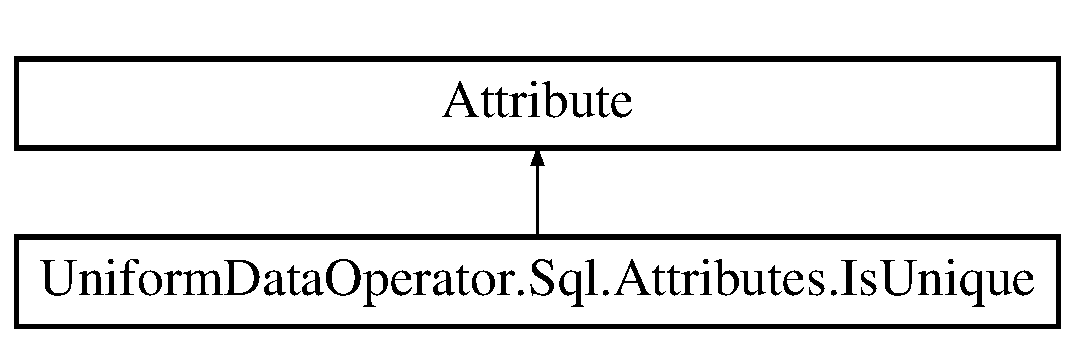
\includegraphics[height=2.000000cm]{d0/d90/class_uniform_data_operator_1_1_sql_1_1_attributes_1_1_is_unique}
\end{center}
\end{figure}
\subsection*{Public Member Functions}
\begin{DoxyCompactItemize}
\item 
string \mbox{\hyperlink{class_uniform_data_operator_1_1_sql_1_1_attributes_1_1_is_unique_aff4e39a64a247b951300a64992c72238}{Unique\+Index\+Declaration\+Command}} (Member\+Info member)
\begin{DoxyCompactList}\small\item\em Return unique index init string. \end{DoxyCompactList}\end{DoxyCompactItemize}


\subsection{Detailed Description}
Is this value must be unique by this column. 



\subsection{Member Function Documentation}
\mbox{\Hypertarget{class_uniform_data_operator_1_1_sql_1_1_attributes_1_1_is_unique_aff4e39a64a247b951300a64992c72238}\label{class_uniform_data_operator_1_1_sql_1_1_attributes_1_1_is_unique_aff4e39a64a247b951300a64992c72238}} 
\index{Uniform\+Data\+Operator\+::\+Sql\+::\+Attributes\+::\+Is\+Unique@{Uniform\+Data\+Operator\+::\+Sql\+::\+Attributes\+::\+Is\+Unique}!Unique\+Index\+Declaration\+Command@{Unique\+Index\+Declaration\+Command}}
\index{Unique\+Index\+Declaration\+Command@{Unique\+Index\+Declaration\+Command}!Uniform\+Data\+Operator\+::\+Sql\+::\+Attributes\+::\+Is\+Unique@{Uniform\+Data\+Operator\+::\+Sql\+::\+Attributes\+::\+Is\+Unique}}
\subsubsection{\texorpdfstring{Unique\+Index\+Declaration\+Command()}{UniqueIndexDeclarationCommand()}}
{\footnotesize\ttfamily string Uniform\+Data\+Operator.\+Sql.\+Attributes.\+Is\+Unique.\+Unique\+Index\+Declaration\+Command (\begin{DoxyParamCaption}\item[{Member\+Info}]{member }\end{DoxyParamCaption})}



Return unique index init string. 

\begin{DoxyReturn}{Returns}

\end{DoxyReturn}


The documentation for this class was generated from the following file\+:\begin{DoxyCompactItemize}
\item 
D\+:/\+Work/\+Git\+Hub/uniform-\/data-\/operator/\+S\+Q\+L/\+Attributes/Is\+Unique.\+cs\end{DoxyCompactItemize}

\hypertarget{class_uniform_data_operator_1_1_sql_1_1_attributes_1_1_is_unsigned}{}\section{Uniform\+Data\+Operator.\+Sql.\+Attributes.\+Is\+Unsigned Class Reference}
\label{class_uniform_data_operator_1_1_sql_1_1_attributes_1_1_is_unsigned}\index{Uniform\+Data\+Operator.\+Sql.\+Attributes.\+Is\+Unsigned@{Uniform\+Data\+Operator.\+Sql.\+Attributes.\+Is\+Unsigned}}


Is not have signs after dot.  


Inheritance diagram for Uniform\+Data\+Operator.\+Sql.\+Attributes.\+Is\+Unsigned\+:\begin{figure}[H]
\begin{center}
\leavevmode
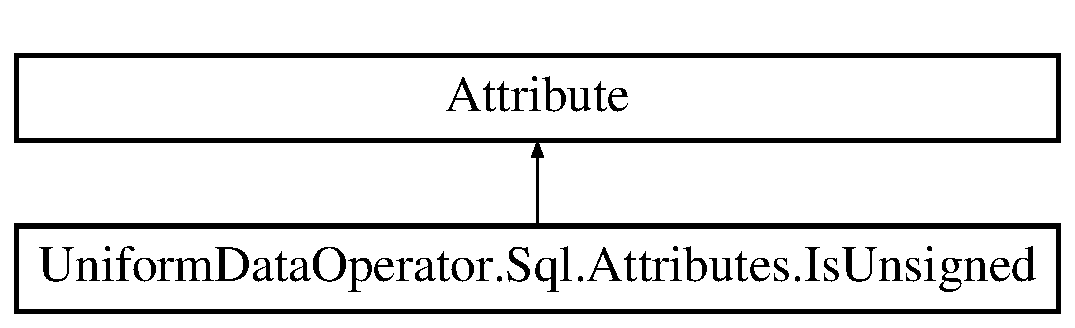
\includegraphics[height=2.000000cm]{d5/d70/class_uniform_data_operator_1_1_sql_1_1_attributes_1_1_is_unsigned}
\end{center}
\end{figure}


\subsection{Detailed Description}
Is not have signs after dot. 



The documentation for this class was generated from the following file\+:\begin{DoxyCompactItemize}
\item 
D\+:/\+Work/\+Git\+Hub/uniform-\/data-\/operator/\+S\+Q\+L/\+Attributes/Is\+Unsigned.\+cs\end{DoxyCompactItemize}

\hypertarget{class_uniform_data_operator_1_1_sql_1_1_attributes_1_1_is_zero_fill}{}\section{Uniform\+Data\+Operator.\+Sql.\+Attributes.\+Is\+Zero\+Fill Class Reference}
\label{class_uniform_data_operator_1_1_sql_1_1_attributes_1_1_is_zero_fill}\index{Uniform\+Data\+Operator.\+Sql.\+Attributes.\+Is\+Zero\+Fill@{Uniform\+Data\+Operator.\+Sql.\+Attributes.\+Is\+Zero\+Fill}}


Is value wold be willed by zero by default. Only for numerical columns.  


Inheritance diagram for Uniform\+Data\+Operator.\+Sql.\+Attributes.\+Is\+Zero\+Fill\+:\begin{figure}[H]
\begin{center}
\leavevmode
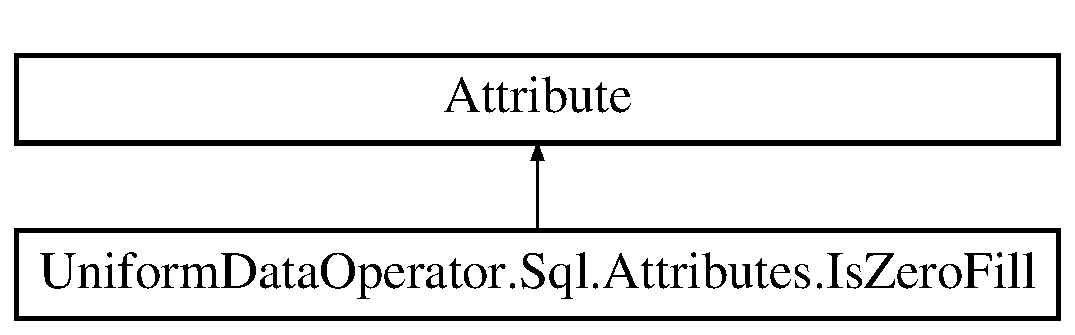
\includegraphics[height=2.000000cm]{d5/d8d/class_uniform_data_operator_1_1_sql_1_1_attributes_1_1_is_zero_fill}
\end{center}
\end{figure}


\subsection{Detailed Description}
Is value wold be willed by zero by default. Only for numerical columns. 



The documentation for this class was generated from the following file\+:\begin{DoxyCompactItemize}
\item 
D\+:/\+Work/\+Git\+Hub/uniform-\/data-\/operator/\+S\+Q\+L/\+Attributes/Is\+Zero\+Fill.\+cs\end{DoxyCompactItemize}

\hypertarget{class_my_s_q_l_tests_1_1_local}{}\section{My\+S\+Q\+L\+Tests.\+Local Class Reference}
\label{class_my_s_q_l_tests_1_1_local}\index{My\+S\+Q\+L\+Tests.\+Local@{My\+S\+Q\+L\+Tests.\+Local}}
\subsection*{Static Public Attributes}
\begin{DoxyCompactItemize}
\item 
\mbox{\Hypertarget{class_my_s_q_l_tests_1_1_local_a19d9d8d0e3af59a0856bba6184a464eb}\label{class_my_s_q_l_tests_1_1_local_a19d9d8d0e3af59a0856bba6184a464eb}} 
static string {\bfseries username} = \char`\"{}root\char`\"{}
\item 
\mbox{\Hypertarget{class_my_s_q_l_tests_1_1_local_ad4430d5a115b43817b9776f2ccbf5633}\label{class_my_s_q_l_tests_1_1_local_ad4430d5a115b43817b9776f2ccbf5633}} 
static string {\bfseries password} = \char`\"{}57182631\+Qbit\char`\"{}
\end{DoxyCompactItemize}


The documentation for this class was generated from the following file\+:\begin{DoxyCompactItemize}
\item 
D\+:/\+Work/\+Git\+Hub/uniform-\/data-\/operator/\+Tests/\+My\+S\+Q\+L\+Tests/Local.\+cs\end{DoxyCompactItemize}

\hypertarget{class_uniform_data_operator_1_1_sql_1_1_my_sql_1_1_my_sql_data_operator}{}\section{Uniform\+Data\+Operator.\+Sql.\+My\+Sql.\+My\+Sql\+Data\+Operator Class Reference}
\label{class_uniform_data_operator_1_1_sql_1_1_my_sql_1_1_my_sql_data_operator}\index{Uniform\+Data\+Operator.\+Sql.\+My\+Sql.\+My\+Sql\+Data\+Operator@{Uniform\+Data\+Operator.\+Sql.\+My\+Sql.\+My\+Sql\+Data\+Operator}}


Operator that provides possibility to operate data on My\+S\+QL data base server.  


Inheritance diagram for Uniform\+Data\+Operator.\+Sql.\+My\+Sql.\+My\+Sql\+Data\+Operator\+:\begin{figure}[H]
\begin{center}
\leavevmode
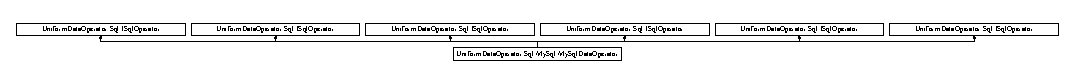
\includegraphics[height=0.590717cm]{d5/d34/class_uniform_data_operator_1_1_sql_1_1_my_sql_1_1_my_sql_data_operator}
\end{center}
\end{figure}
\subsection*{Public Member Functions}
\begin{DoxyCompactItemize}
\item 
void \mbox{\hyperlink{class_uniform_data_operator_1_1_sql_1_1_my_sql_1_1_my_sql_data_operator_a0dbd58206733a17dd26143b58d0859d7}{Backup}} (string directory)
\begin{DoxyCompactList}\small\item\em Backuping data base to sql file in directory. Name would be generated by timestamp. \end{DoxyCompactList}\item 
void \mbox{\hyperlink{class_uniform_data_operator_1_1_sql_1_1_my_sql_1_1_my_sql_data_operator_a22a9e92989ebdb3a52b8ebe409c59831}{Restore}} (string file\+Path)
\begin{DoxyCompactList}\small\item\em Restoring S\+QL db from file. \end{DoxyCompactList}\item 
bool \mbox{\hyperlink{class_uniform_data_operator_1_1_sql_1_1_my_sql_1_1_my_sql_data_operator_a2ed7d06bc016ae6d07cbcceffc21bbd3}{Activate\+Schema}} (string schema\+Name, out string error)
\begin{DoxyCompactList}\small\item\em Trying to set schema to databases server in case if schema not exist. \end{DoxyCompactList}\item 
string \mbox{\hyperlink{class_uniform_data_operator_1_1_sql_1_1_my_sql_1_1_my_sql_data_operator_a0bdc2943e5d10576fb564913cdd744e7}{Column\+Declaration\+Command}} (Member\+Info member)
\begin{DoxyCompactList}\small\item\em Return generated S\+QL command relative to init time. \end{DoxyCompactList}\item 
Db\+Command \mbox{\hyperlink{class_uniform_data_operator_1_1_sql_1_1_my_sql_1_1_my_sql_data_operator_ac3af074cabe5721a685f0650dc69a871}{Generate\+Set\+To\+Table\+Command}} (Type table\+Type, object data, out string error)
\begin{DoxyCompactList}\small\item\em Generating set to table sql command from provided source data. \end{DoxyCompactList}\item 
bool \mbox{\hyperlink{class_uniform_data_operator_1_1_sql_1_1_my_sql_1_1_my_sql_data_operator_ac1bee965fd57e9b2949c09a6b72a9e3e}{Set\+To\+Table$<$ T $>$}} (object data, out string error)
\begin{DoxyCompactList}\small\item\em Creating request that setting up data from object to data base server acording to attributes. \end{DoxyCompactList}\item 
bool \mbox{\hyperlink{class_uniform_data_operator_1_1_sql_1_1_my_sql_1_1_my_sql_data_operator_a5a12c84883a7e4945b4fb3787a39b302}{Set\+To\+Table}} (Type table\+Type, object data, out string error)
\begin{DoxyCompactList}\small\item\em Creating request that setting up data from object to data base server acording to attributes. \end{DoxyCompactList}\item 
async Task \mbox{\hyperlink{class_uniform_data_operator_1_1_sql_1_1_my_sql_1_1_my_sql_data_operator_ac615a17b6330b292dcf3fd912e1f4fe2}{Set\+To\+Table\+Async$<$ T $>$}} (Cancellation\+Token cancellation\+Token, object data)
\begin{DoxyCompactList}\small\item\em Creating request that setting up data from object to data base server acording to attributes. \end{DoxyCompactList}\item 
async Task \mbox{\hyperlink{class_uniform_data_operator_1_1_sql_1_1_my_sql_1_1_my_sql_data_operator_a036b234868363f2f680e5157ee459439}{Set\+To\+Table\+Async}} (Type table\+Type, Cancellation\+Token cancellation\+Token, object data)
\begin{DoxyCompactList}\small\item\em Creating request that setting up data from object to data base server acording to attributes. \end{DoxyCompactList}\item 
bool \mbox{\hyperlink{class_uniform_data_operator_1_1_sql_1_1_my_sql_1_1_my_sql_data_operator_ae7ad4f4d29d927fa8551b087a6e596b5}{Open\+Connection}} (out string error)
\begin{DoxyCompactList}\small\item\em Opening connection to S\+QL server. \end{DoxyCompactList}\item 
bool \mbox{\hyperlink{class_uniform_data_operator_1_1_sql_1_1_my_sql_1_1_my_sql_data_operator_ae096306ef55611afbe96b0017f2032f6}{Close\+Connection}} ()
\begin{DoxyCompactList}\small\item\em Closing connection to S\+QL server. \end{DoxyCompactList}\item 
bool \mbox{\hyperlink{class_uniform_data_operator_1_1_sql_1_1_my_sql_1_1_my_sql_data_operator_a8f44635dc337c3652041f079190a792d}{Set\+To\+Object}} (Type table\+Type, object obj, out string error, string\mbox{[}$\,$\mbox{]} select, params string\mbox{[}$\,$\mbox{]} where)
\begin{DoxyCompactList}\small\item\em Trying to set object data to database. \end{DoxyCompactList}\item 
bool \mbox{\hyperlink{class_uniform_data_operator_1_1_sql_1_1_my_sql_1_1_my_sql_data_operator_af763205fa1d8a8ad83afc672d5743d65}{Set\+To\+Object}} (Type table\+Type, object obj, out string error, params string\mbox{[}$\,$\mbox{]} select)
\begin{DoxyCompactList}\small\item\em Trying to set object data to database. Automaticly build where block with primary keys. \end{DoxyCompactList}\item 
bool \mbox{\hyperlink{class_uniform_data_operator_1_1_sql_1_1_my_sql_1_1_my_sql_data_operator_a5da5cc531c8c953f73e7fc50513790e9}{Set\+To\+Object}} (Type table\+Type, object obj, out string error)
\begin{DoxyCompactList}\small\item\em Trying to set object data to database. Automaticly build where block with primary keys. Select all available columns. \end{DoxyCompactList}\item 
bool \mbox{\hyperlink{class_uniform_data_operator_1_1_sql_1_1_my_sql_1_1_my_sql_data_operator_a38d9367d43538c2afc77331fe18ab666}{Set\+To\+Objects}} (Type table\+Type, object obj, out I\+List collection, out string error, string\mbox{[}$\,$\mbox{]} select, params string\mbox{[}$\,$\mbox{]} where)
\begin{DoxyCompactList}\small\item\em Setting data from DB Data reader to object by using column map described at object Type. Auto-\/generate S\+QL query and request coluns data relative to privary keys described in object. \end{DoxyCompactList}\item 
bool \mbox{\hyperlink{class_uniform_data_operator_1_1_sql_1_1_my_sql_1_1_my_sql_data_operator_a26b72128803de85e9c44ac6deecc78c4}{Set\+To\+Objects}} (Type table\+Type, object obj, out I\+List collection, out string error, params string\mbox{[}$\,$\mbox{]} select)
\begin{DoxyCompactList}\small\item\em Setting data from DB Data reader to object by using column map described at object Type. Auto-\/generate S\+QL query and request coluns data relative to privary keys described in object. \end{DoxyCompactList}\item 
bool \mbox{\hyperlink{class_uniform_data_operator_1_1_sql_1_1_my_sql_1_1_my_sql_data_operator_a4079de461f0a37c0b69754a0e93dc05b}{Set\+To\+Objects}} (Type table\+Type, object obj, out I\+List collection, out string error)
\begin{DoxyCompactList}\small\item\em Setting data from DB Data reader to object by using column map described at object Type. Auto-\/generate S\+QL query and request coluns data relative to privary keys described in object. \end{DoxyCompactList}\item 
async Task \mbox{\hyperlink{class_uniform_data_operator_1_1_sql_1_1_my_sql_1_1_my_sql_data_operator_a98b579ed4a87c3f9dbdb90ffc28bf15c}{Set\+To\+Object\+Async}} (Type table\+Type, Cancellation\+Token cancellation\+Token, object obj, string\mbox{[}$\,$\mbox{]} select, params string\mbox{[}$\,$\mbox{]} where)
\begin{DoxyCompactList}\small\item\em Trying to set object data to database. \end{DoxyCompactList}\item 
async Task \mbox{\hyperlink{class_uniform_data_operator_1_1_sql_1_1_my_sql_1_1_my_sql_data_operator_a49ee22a2a69fbc0752c989c7b79e5e43}{Set\+To\+Object\+Async}} (Type table\+Type, Cancellation\+Token cancellation\+Token, object obj, params string\mbox{[}$\,$\mbox{]} select)
\begin{DoxyCompactList}\small\item\em Trying to set object data to database. \end{DoxyCompactList}\item 
async Task \mbox{\hyperlink{class_uniform_data_operator_1_1_sql_1_1_my_sql_1_1_my_sql_data_operator_a3be9aeb9ce11e3fd536449843a585490}{Set\+To\+Object\+Async}} (Type table\+Type, Cancellation\+Token cancellation\+Token, object obj)
\begin{DoxyCompactList}\small\item\em Trying to set object data to database. \end{DoxyCompactList}\item 
async Task \mbox{\hyperlink{class_uniform_data_operator_1_1_sql_1_1_my_sql_1_1_my_sql_data_operator_a5fc9ae81932a2d5259dd817e91593988}{Set\+To\+Objects\+Async}} (Type table\+Type, Cancellation\+Token cancellation\+Token, object obj, System.\+Action$<$ I\+List $>$ callback, string\mbox{[}$\,$\mbox{]} select, params string\mbox{[}$\,$\mbox{]} where)
\begin{DoxyCompactList}\small\item\em Setting data from DB Data reader to object by using column map described at object Type. Auto-\/generate S\+QL query and request coluns data relative to privary keys described in object. \end{DoxyCompactList}\item 
async Task \mbox{\hyperlink{class_uniform_data_operator_1_1_sql_1_1_my_sql_1_1_my_sql_data_operator_a1ca50c33ecedb751642e77668da5229f}{Set\+To\+Objects\+Async}} (Type table\+Type, Cancellation\+Token cancellation\+Token, object obj, System.\+Action$<$ I\+List $>$ callback, params string\mbox{[}$\,$\mbox{]} select)
\begin{DoxyCompactList}\small\item\em Setting data from DB Data reader to object by using column map described at object Type. Auto-\/generate S\+QL query and request coluns data relative to privary keys described in object. \end{DoxyCompactList}\item 
async Task \mbox{\hyperlink{class_uniform_data_operator_1_1_sql_1_1_my_sql_1_1_my_sql_data_operator_a28cf5d9cf061019b0e7da5d966c8db63}{Set\+To\+Objects\+Async}} (Type table\+Type, Cancellation\+Token cancellation\+Token, object obj, System.\+Action$<$ I\+List $>$ callback)
\begin{DoxyCompactList}\small\item\em Setting data from DB Data reader to object by using column map described at object Type. Auto-\/generate S\+QL query and request coluns data relative to privary keys described in object. \end{DoxyCompactList}\item 
void \mbox{\hyperlink{class_uniform_data_operator_1_1_sql_1_1_my_sql_1_1_my_sql_data_operator_a5aad834d2ceba598037b6ed19b27db6d}{Initialize}} ()
\begin{DoxyCompactList}\small\item\em Initialize My\+Sql\+Connection. \end{DoxyCompactList}\item 
Db\+Command \mbox{\hyperlink{class_uniform_data_operator_1_1_sql_1_1_my_sql_1_1_my_sql_data_operator_af5850bfb38f7dfcd5acd5157458ef4bd}{New\+Command}} ()
\begin{DoxyCompactList}\small\item\em Return new clear command suitable for current DB. \end{DoxyCompactList}\item 
Db\+Command \mbox{\hyperlink{class_uniform_data_operator_1_1_sql_1_1_my_sql_1_1_my_sql_data_operator_a6c2e2d374072c275953a515379963881}{New\+Command}} (string command\+Text)
\begin{DoxyCompactList}\small\item\em Return new clear command suitable for current DB with included command text. \end{DoxyCompactList}\item 
Db\+Command \mbox{\hyperlink{class_uniform_data_operator_1_1_sql_1_1_my_sql_1_1_my_sql_data_operator_affbacb4fb1773fc14cdbb9cbcd315c5f}{Disable\+Sql\+Checks}} (Db\+Command command)
\begin{DoxyCompactList}\small\item\em Add code that disabling S\+QL checks during executing command. \end{DoxyCompactList}\item 
string \mbox{\hyperlink{class_uniform_data_operator_1_1_sql_1_1_my_sql_1_1_my_sql_data_operator_a3e80f9136c9fef46a443901a15f1e289}{Disable\+Sql\+Checks}} (string command)
\begin{DoxyCompactList}\small\item\em Add code that disabling S\+QL checks during executing command. \end{DoxyCompactList}\item 
bool \mbox{\hyperlink{class_uniform_data_operator_1_1_sql_1_1_my_sql_1_1_my_sql_data_operator_a233ab791c68b93aded97bfd9986767e8}{Validate\+Table\+Member}} (\mbox{\hyperlink{class_uniform_data_operator_1_1_sql_1_1_attributes_1_1_table}{Table}} table\+Descriptor, Member\+Info column\+Member)
\begin{DoxyCompactList}\small\item\em Validate data base table column acording to member attributes. \end{DoxyCompactList}\item 
Db\+Parameter \mbox{\hyperlink{class_uniform_data_operator_1_1_sql_1_1_my_sql_1_1_my_sql_data_operator_a7d10fc1dfc16ece78ad066f596523782}{Member\+To\+Parameter}} (object data, \mbox{\hyperlink{class_uniform_data_operator_1_1_sql_1_1_attributes_1_1_column}{Column}} column)
\begin{DoxyCompactList}\small\item\em Convert value of member to data base parameter that can be used in command. \end{DoxyCompactList}\item 
string \mbox{\hyperlink{class_uniform_data_operator_1_1_sql_1_1_my_sql_1_1_my_sql_data_operator_a7b854ebbcdf31c67716d8c365c321a31}{Db\+Type\+To\+String}} (Db\+Type type)
\begin{DoxyCompactList}\small\item\em Trying to convert D\+B\+Type to specified type in string format that suitable to this database. \end{DoxyCompactList}\end{DoxyCompactItemize}
\subsection*{Properties}
\begin{DoxyCompactItemize}
\item 
static \mbox{\hyperlink{class_uniform_data_operator_1_1_sql_1_1_my_sql_1_1_my_sql_data_operator}{My\+Sql\+Data\+Operator}} \mbox{\hyperlink{class_uniform_data_operator_1_1_sql_1_1_my_sql_1_1_my_sql_data_operator_a8e8f8f936f6a4306dc4dc0d3eb07770c}{Active}}\hspace{0.3cm}{\ttfamily  \mbox{[}get\mbox{]}}
\begin{DoxyCompactList}\small\item\em Active single tone instance of My\+S\+QL data provider. \end{DoxyCompactList}\item 
string \mbox{\hyperlink{class_uniform_data_operator_1_1_sql_1_1_my_sql_1_1_my_sql_data_operator_a2154fef9e522ef26cf08642483fed223}{Server}} = \char`\"{}127.\+0.\+0.\+1\char`\"{}\hspace{0.3cm}{\ttfamily  \mbox{[}get, set\mbox{]}}
\begin{DoxyCompactList}\small\item\em Server\textquotesingle{}s ip. \end{DoxyCompactList}\item 
int \mbox{\hyperlink{class_uniform_data_operator_1_1_sql_1_1_my_sql_1_1_my_sql_data_operator_a2cfc65d2842491734270dfe114d9eec5}{Port}} = 3306\hspace{0.3cm}{\ttfamily  \mbox{[}get, set\mbox{]}}
\begin{DoxyCompactList}\small\item\em Port for server access. \end{DoxyCompactList}\item 
string \mbox{\hyperlink{class_uniform_data_operator_1_1_sql_1_1_my_sql_1_1_my_sql_data_operator_a144616e12acb2b55c7046af0c9af989d}{Database}}\hspace{0.3cm}{\ttfamily  \mbox{[}get, set\mbox{]}}
\begin{DoxyCompactList}\small\item\em Database\textquotesingle{}s name. \end{DoxyCompactList}\item 
string \mbox{\hyperlink{class_uniform_data_operator_1_1_sql_1_1_my_sql_1_1_my_sql_data_operator_ae5e119508a6d9807b9e138c628a6e18f}{User\+Id}}\hspace{0.3cm}{\ttfamily  \mbox{[}get, set\mbox{]}}
\begin{DoxyCompactList}\small\item\em User for connection. \end{DoxyCompactList}\item 
string \mbox{\hyperlink{class_uniform_data_operator_1_1_sql_1_1_my_sql_1_1_my_sql_data_operator_aa080c79169d2bf29ac2249436ef2471c}{Password}}\hspace{0.3cm}{\ttfamily  \mbox{[}get, set\mbox{]}}
\begin{DoxyCompactList}\small\item\em User\textquotesingle{}s password. \end{DoxyCompactList}\item 
Db\+Connection \mbox{\hyperlink{class_uniform_data_operator_1_1_sql_1_1_my_sql_1_1_my_sql_data_operator_a5c5d34c3f7b7d95773ba44ede46409a0}{Connection}}\hspace{0.3cm}{\ttfamily  \mbox{[}get\mbox{]}}
\begin{DoxyCompactList}\small\item\em Connection to DB. \end{DoxyCompactList}\end{DoxyCompactItemize}
\subsection*{Static Private Member Functions}
\begin{DoxyCompactItemize}
\item 
static bool \mbox{\hyperlink{class_uniform_data_operator_1_1_sql_1_1_my_sql_1_1_my_sql_data_operator_a821d08d641098b3f5e4dd6342a3db718}{Validate\+Entry\+RD}} (Type table\+Type, object obj, out string error)
\begin{DoxyCompactList}\small\item\em Validate entry data for read query. \end{DoxyCompactList}\item 
static List$<$ Member\+Info $>$ \mbox{\hyperlink{class_uniform_data_operator_1_1_sql_1_1_my_sql_1_1_my_sql_data_operator_ad6b8397c665d57eac1a2680c7b5f44e9}{Members\+Allowed\+To\+Set}} (Type table\+Type, object obj, out string error)
\begin{DoxyCompactList}\small\item\em Detect common collection of members that can be included to query. \end{DoxyCompactList}\item 
static Db\+Command \mbox{\hyperlink{class_uniform_data_operator_1_1_sql_1_1_my_sql_1_1_my_sql_data_operator_a0d3153822bac0ad760aed9f37e58d69b}{Generate\+Set\+To\+Object\+Command}} (Type table\+Type, object obj, I\+Enumerable$<$ Member\+Info $>$ where, I\+Enumerable$<$ Member\+Info $>$ select)
\begin{DoxyCompactList}\small\item\em Trying to generate command that would request objects members from server. \end{DoxyCompactList}\item 
static bool \mbox{\hyperlink{class_uniform_data_operator_1_1_sql_1_1_my_sql_1_1_my_sql_data_operator_a30fd1063d13dae2c7833aed7c405554c}{Detect\+P\+K\+To\+Set}} (Type table\+Type, out string error, out string\mbox{[}$\,$\mbox{]} pks\+Array)
\begin{DoxyCompactList}\small\item\em Looking for primary keys in table and build them names to array. \end{DoxyCompactList}\end{DoxyCompactItemize}
\subsection*{Private Attributes}
\begin{DoxyCompactItemize}
\item 
My\+Sql\+Connection \mbox{\hyperlink{class_uniform_data_operator_1_1_sql_1_1_my_sql_1_1_my_sql_data_operator_a807f034631cd8284ecc020d765e6f6f1}{connection}}
\begin{DoxyCompactList}\small\item\em Object that managing connection with DB. \end{DoxyCompactList}\end{DoxyCompactItemize}


\subsection{Detailed Description}
Operator that provides possibility to operate data on My\+S\+QL data base server. 



\subsection{Member Function Documentation}
\mbox{\Hypertarget{class_uniform_data_operator_1_1_sql_1_1_my_sql_1_1_my_sql_data_operator_a2ed7d06bc016ae6d07cbcceffc21bbd3}\label{class_uniform_data_operator_1_1_sql_1_1_my_sql_1_1_my_sql_data_operator_a2ed7d06bc016ae6d07cbcceffc21bbd3}} 
\index{Uniform\+Data\+Operator\+::\+Sql\+::\+My\+Sql\+::\+My\+Sql\+Data\+Operator@{Uniform\+Data\+Operator\+::\+Sql\+::\+My\+Sql\+::\+My\+Sql\+Data\+Operator}!Activate\+Schema@{Activate\+Schema}}
\index{Activate\+Schema@{Activate\+Schema}!Uniform\+Data\+Operator\+::\+Sql\+::\+My\+Sql\+::\+My\+Sql\+Data\+Operator@{Uniform\+Data\+Operator\+::\+Sql\+::\+My\+Sql\+::\+My\+Sql\+Data\+Operator}}
\subsubsection{\texorpdfstring{Activate\+Schema()}{ActivateSchema()}}
{\footnotesize\ttfamily bool Uniform\+Data\+Operator.\+Sql.\+My\+Sql.\+My\+Sql\+Data\+Operator.\+Activate\+Schema (\begin{DoxyParamCaption}\item[{string}]{schema\+Name,  }\item[{out string}]{error }\end{DoxyParamCaption})}



Trying to set schema to databases server in case if schema not exist. 


\begin{DoxyParams}{Parameters}
{\em schema\+Name} & Name of the schema that would be used.\\
\hline
{\em error} & Error faces during operation.\\
\hline
\end{DoxyParams}
\begin{DoxyReturn}{Returns}

\end{DoxyReturn}


Implements \mbox{\hyperlink{interface_uniform_data_operator_1_1_sql_1_1_i_sql_operator_a5ae8328a464ef80f1ae1bd46a573c265}{Uniform\+Data\+Operator.\+Sql.\+I\+Sql\+Operator}}.

\mbox{\Hypertarget{class_uniform_data_operator_1_1_sql_1_1_my_sql_1_1_my_sql_data_operator_a0dbd58206733a17dd26143b58d0859d7}\label{class_uniform_data_operator_1_1_sql_1_1_my_sql_1_1_my_sql_data_operator_a0dbd58206733a17dd26143b58d0859d7}} 
\index{Uniform\+Data\+Operator\+::\+Sql\+::\+My\+Sql\+::\+My\+Sql\+Data\+Operator@{Uniform\+Data\+Operator\+::\+Sql\+::\+My\+Sql\+::\+My\+Sql\+Data\+Operator}!Backup@{Backup}}
\index{Backup@{Backup}!Uniform\+Data\+Operator\+::\+Sql\+::\+My\+Sql\+::\+My\+Sql\+Data\+Operator@{Uniform\+Data\+Operator\+::\+Sql\+::\+My\+Sql\+::\+My\+Sql\+Data\+Operator}}
\subsubsection{\texorpdfstring{Backup()}{Backup()}}
{\footnotesize\ttfamily void Uniform\+Data\+Operator.\+Sql.\+My\+Sql.\+My\+Sql\+Data\+Operator.\+Backup (\begin{DoxyParamCaption}\item[{string}]{directory }\end{DoxyParamCaption})}



Backuping data base to sql file in directory. Name would be generated by timestamp. 


\begin{DoxyParams}{Parameters}
{\em directory} & Directory that would store the backup file.\\
\hline
\end{DoxyParams}


Implements \mbox{\hyperlink{interface_uniform_data_operator_1_1_sql_1_1_i_sql_operator_a096be4f746c1fcbb8b2894c2517b937c}{Uniform\+Data\+Operator.\+Sql.\+I\+Sql\+Operator}}.

\mbox{\Hypertarget{class_uniform_data_operator_1_1_sql_1_1_my_sql_1_1_my_sql_data_operator_ae096306ef55611afbe96b0017f2032f6}\label{class_uniform_data_operator_1_1_sql_1_1_my_sql_1_1_my_sql_data_operator_ae096306ef55611afbe96b0017f2032f6}} 
\index{Uniform\+Data\+Operator\+::\+Sql\+::\+My\+Sql\+::\+My\+Sql\+Data\+Operator@{Uniform\+Data\+Operator\+::\+Sql\+::\+My\+Sql\+::\+My\+Sql\+Data\+Operator}!Close\+Connection@{Close\+Connection}}
\index{Close\+Connection@{Close\+Connection}!Uniform\+Data\+Operator\+::\+Sql\+::\+My\+Sql\+::\+My\+Sql\+Data\+Operator@{Uniform\+Data\+Operator\+::\+Sql\+::\+My\+Sql\+::\+My\+Sql\+Data\+Operator}}
\subsubsection{\texorpdfstring{Close\+Connection()}{CloseConnection()}}
{\footnotesize\ttfamily bool Uniform\+Data\+Operator.\+Sql.\+My\+Sql.\+My\+Sql\+Data\+Operator.\+Close\+Connection (\begin{DoxyParamCaption}{ }\end{DoxyParamCaption})}



Closing connection to S\+QL server. 

\begin{DoxyReturn}{Returns}
Result of connection closing.
\end{DoxyReturn}


Implements \mbox{\hyperlink{interface_uniform_data_operator_1_1_sql_1_1_i_sql_operator_a1a6429996e1bbb452f4e034fd634e640}{Uniform\+Data\+Operator.\+Sql.\+I\+Sql\+Operator}}.

\mbox{\Hypertarget{class_uniform_data_operator_1_1_sql_1_1_my_sql_1_1_my_sql_data_operator_a0bdc2943e5d10576fb564913cdd744e7}\label{class_uniform_data_operator_1_1_sql_1_1_my_sql_1_1_my_sql_data_operator_a0bdc2943e5d10576fb564913cdd744e7}} 
\index{Uniform\+Data\+Operator\+::\+Sql\+::\+My\+Sql\+::\+My\+Sql\+Data\+Operator@{Uniform\+Data\+Operator\+::\+Sql\+::\+My\+Sql\+::\+My\+Sql\+Data\+Operator}!Column\+Declaration\+Command@{Column\+Declaration\+Command}}
\index{Column\+Declaration\+Command@{Column\+Declaration\+Command}!Uniform\+Data\+Operator\+::\+Sql\+::\+My\+Sql\+::\+My\+Sql\+Data\+Operator@{Uniform\+Data\+Operator\+::\+Sql\+::\+My\+Sql\+::\+My\+Sql\+Data\+Operator}}
\subsubsection{\texorpdfstring{Column\+Declaration\+Command()}{ColumnDeclarationCommand()}}
{\footnotesize\ttfamily string Uniform\+Data\+Operator.\+Sql.\+My\+Sql.\+My\+Sql\+Data\+Operator.\+Column\+Declaration\+Command (\begin{DoxyParamCaption}\item[{Member\+Info}]{member }\end{DoxyParamCaption})}



Return generated S\+QL command relative to init time. 


\begin{DoxyParams}{Parameters}
{\em member} & Member that contains defined attributes that describes column definition.\\
\hline
\end{DoxyParams}
\begin{DoxyReturn}{Returns}
S\+QL command relative to \mbox{\hyperlink{namespace_uniform_data_operator_1_1_sql_1_1_my_sql}{My\+Sql}} server.
\end{DoxyReturn}


Implements \mbox{\hyperlink{interface_uniform_data_operator_1_1_sql_1_1_i_sql_operator_aac9c3ed1e73af66e383340a154786ec7}{Uniform\+Data\+Operator.\+Sql.\+I\+Sql\+Operator}}.

\mbox{\Hypertarget{class_uniform_data_operator_1_1_sql_1_1_my_sql_1_1_my_sql_data_operator_a7b854ebbcdf31c67716d8c365c321a31}\label{class_uniform_data_operator_1_1_sql_1_1_my_sql_1_1_my_sql_data_operator_a7b854ebbcdf31c67716d8c365c321a31}} 
\index{Uniform\+Data\+Operator\+::\+Sql\+::\+My\+Sql\+::\+My\+Sql\+Data\+Operator@{Uniform\+Data\+Operator\+::\+Sql\+::\+My\+Sql\+::\+My\+Sql\+Data\+Operator}!Db\+Type\+To\+String@{Db\+Type\+To\+String}}
\index{Db\+Type\+To\+String@{Db\+Type\+To\+String}!Uniform\+Data\+Operator\+::\+Sql\+::\+My\+Sql\+::\+My\+Sql\+Data\+Operator@{Uniform\+Data\+Operator\+::\+Sql\+::\+My\+Sql\+::\+My\+Sql\+Data\+Operator}}
\subsubsection{\texorpdfstring{Db\+Type\+To\+String()}{DbTypeToString()}}
{\footnotesize\ttfamily string Uniform\+Data\+Operator.\+Sql.\+My\+Sql.\+My\+Sql\+Data\+Operator.\+Db\+Type\+To\+String (\begin{DoxyParamCaption}\item[{Db\+Type}]{type }\end{DoxyParamCaption})}



Trying to convert D\+B\+Type to specified type in string format that suitable to this database. 


\begin{DoxyParams}{Parameters}
{\em type} & Common D\+B\+Type.\\
\hline
\end{DoxyParams}
\begin{DoxyReturn}{Returns}
Type suitable for S\+QL command relative to this type of data base. Invalid\+Cast\+Exception in case if converting not possible.
\end{DoxyReturn}


Implements \mbox{\hyperlink{interface_uniform_data_operator_1_1_sql_1_1_i_sql_operator_a51af40df39808d53cdcc81852b836634}{Uniform\+Data\+Operator.\+Sql.\+I\+Sql\+Operator}}.

\mbox{\Hypertarget{class_uniform_data_operator_1_1_sql_1_1_my_sql_1_1_my_sql_data_operator_a30fd1063d13dae2c7833aed7c405554c}\label{class_uniform_data_operator_1_1_sql_1_1_my_sql_1_1_my_sql_data_operator_a30fd1063d13dae2c7833aed7c405554c}} 
\index{Uniform\+Data\+Operator\+::\+Sql\+::\+My\+Sql\+::\+My\+Sql\+Data\+Operator@{Uniform\+Data\+Operator\+::\+Sql\+::\+My\+Sql\+::\+My\+Sql\+Data\+Operator}!Detect\+P\+K\+To\+Set@{Detect\+P\+K\+To\+Set}}
\index{Detect\+P\+K\+To\+Set@{Detect\+P\+K\+To\+Set}!Uniform\+Data\+Operator\+::\+Sql\+::\+My\+Sql\+::\+My\+Sql\+Data\+Operator@{Uniform\+Data\+Operator\+::\+Sql\+::\+My\+Sql\+::\+My\+Sql\+Data\+Operator}}
\subsubsection{\texorpdfstring{Detect\+P\+K\+To\+Set()}{DetectPKToSet()}}
{\footnotesize\ttfamily static bool Uniform\+Data\+Operator.\+Sql.\+My\+Sql.\+My\+Sql\+Data\+Operator.\+Detect\+P\+K\+To\+Set (\begin{DoxyParamCaption}\item[{Type}]{table\+Type,  }\item[{out string}]{error,  }\item[{out string \mbox{[}$\,$\mbox{]}}]{pks\+Array }\end{DoxyParamCaption})\hspace{0.3cm}{\ttfamily [static]}, {\ttfamily [private]}}



Looking for primary keys in table and build them names to array. 


\begin{DoxyParams}{Parameters}
{\em table\+Type} & Type that describe table.\\
\hline
{\em error} & Error if occured. Null if operation success.\\
\hline
{\em pks\+Array} & Output arrey that contains names of PK columns.\\
\hline
\end{DoxyParams}
\begin{DoxyReturn}{Returns}

\end{DoxyReturn}
\mbox{\Hypertarget{class_uniform_data_operator_1_1_sql_1_1_my_sql_1_1_my_sql_data_operator_affbacb4fb1773fc14cdbb9cbcd315c5f}\label{class_uniform_data_operator_1_1_sql_1_1_my_sql_1_1_my_sql_data_operator_affbacb4fb1773fc14cdbb9cbcd315c5f}} 
\index{Uniform\+Data\+Operator\+::\+Sql\+::\+My\+Sql\+::\+My\+Sql\+Data\+Operator@{Uniform\+Data\+Operator\+::\+Sql\+::\+My\+Sql\+::\+My\+Sql\+Data\+Operator}!Disable\+Sql\+Checks@{Disable\+Sql\+Checks}}
\index{Disable\+Sql\+Checks@{Disable\+Sql\+Checks}!Uniform\+Data\+Operator\+::\+Sql\+::\+My\+Sql\+::\+My\+Sql\+Data\+Operator@{Uniform\+Data\+Operator\+::\+Sql\+::\+My\+Sql\+::\+My\+Sql\+Data\+Operator}}
\subsubsection{\texorpdfstring{Disable\+Sql\+Checks()}{DisableSqlChecks()}\hspace{0.1cm}{\footnotesize\ttfamily [1/2]}}
{\footnotesize\ttfamily Db\+Command Uniform\+Data\+Operator.\+Sql.\+My\+Sql.\+My\+Sql\+Data\+Operator.\+Disable\+Sql\+Checks (\begin{DoxyParamCaption}\item[{Db\+Command}]{command }\end{DoxyParamCaption})}



Add code that disabling S\+QL checks during executing command. 


\begin{DoxyParams}{Parameters}
{\em command} & Target command that would be modified during operation.\\
\hline
\end{DoxyParams}
\begin{DoxyReturn}{Returns}
Modified comand.
\end{DoxyReturn}


Implements \mbox{\hyperlink{interface_uniform_data_operator_1_1_sql_1_1_i_sql_operator_a12d464e0532a3e194b1221eee0c32d34}{Uniform\+Data\+Operator.\+Sql.\+I\+Sql\+Operator}}.

\mbox{\Hypertarget{class_uniform_data_operator_1_1_sql_1_1_my_sql_1_1_my_sql_data_operator_a3e80f9136c9fef46a443901a15f1e289}\label{class_uniform_data_operator_1_1_sql_1_1_my_sql_1_1_my_sql_data_operator_a3e80f9136c9fef46a443901a15f1e289}} 
\index{Uniform\+Data\+Operator\+::\+Sql\+::\+My\+Sql\+::\+My\+Sql\+Data\+Operator@{Uniform\+Data\+Operator\+::\+Sql\+::\+My\+Sql\+::\+My\+Sql\+Data\+Operator}!Disable\+Sql\+Checks@{Disable\+Sql\+Checks}}
\index{Disable\+Sql\+Checks@{Disable\+Sql\+Checks}!Uniform\+Data\+Operator\+::\+Sql\+::\+My\+Sql\+::\+My\+Sql\+Data\+Operator@{Uniform\+Data\+Operator\+::\+Sql\+::\+My\+Sql\+::\+My\+Sql\+Data\+Operator}}
\subsubsection{\texorpdfstring{Disable\+Sql\+Checks()}{DisableSqlChecks()}\hspace{0.1cm}{\footnotesize\ttfamily [2/2]}}
{\footnotesize\ttfamily string Uniform\+Data\+Operator.\+Sql.\+My\+Sql.\+My\+Sql\+Data\+Operator.\+Disable\+Sql\+Checks (\begin{DoxyParamCaption}\item[{string}]{command }\end{DoxyParamCaption})}



Add code that disabling S\+QL checks during executing command. 


\begin{DoxyParams}{Parameters}
{\em command} & Target command that would be modified during operation.\\
\hline
\end{DoxyParams}
\begin{DoxyReturn}{Returns}
Modified comand.
\end{DoxyReturn}


Implements \mbox{\hyperlink{interface_uniform_data_operator_1_1_sql_1_1_i_sql_operator_a0757f304a24ffaa743e23e8bdd210950}{Uniform\+Data\+Operator.\+Sql.\+I\+Sql\+Operator}}.

\mbox{\Hypertarget{class_uniform_data_operator_1_1_sql_1_1_my_sql_1_1_my_sql_data_operator_a0d3153822bac0ad760aed9f37e58d69b}\label{class_uniform_data_operator_1_1_sql_1_1_my_sql_1_1_my_sql_data_operator_a0d3153822bac0ad760aed9f37e58d69b}} 
\index{Uniform\+Data\+Operator\+::\+Sql\+::\+My\+Sql\+::\+My\+Sql\+Data\+Operator@{Uniform\+Data\+Operator\+::\+Sql\+::\+My\+Sql\+::\+My\+Sql\+Data\+Operator}!Generate\+Set\+To\+Object\+Command@{Generate\+Set\+To\+Object\+Command}}
\index{Generate\+Set\+To\+Object\+Command@{Generate\+Set\+To\+Object\+Command}!Uniform\+Data\+Operator\+::\+Sql\+::\+My\+Sql\+::\+My\+Sql\+Data\+Operator@{Uniform\+Data\+Operator\+::\+Sql\+::\+My\+Sql\+::\+My\+Sql\+Data\+Operator}}
\subsubsection{\texorpdfstring{Generate\+Set\+To\+Object\+Command()}{GenerateSetToObjectCommand()}}
{\footnotesize\ttfamily static Db\+Command Uniform\+Data\+Operator.\+Sql.\+My\+Sql.\+My\+Sql\+Data\+Operator.\+Generate\+Set\+To\+Object\+Command (\begin{DoxyParamCaption}\item[{Type}]{table\+Type,  }\item[{object}]{obj,  }\item[{I\+Enumerable$<$ Member\+Info $>$}]{where,  }\item[{I\+Enumerable$<$ Member\+Info $>$}]{select }\end{DoxyParamCaption})\hspace{0.3cm}{\ttfamily [static]}, {\ttfamily [private]}}



Trying to generate command that would request objects members from server. 


\begin{DoxyParams}{Parameters}
{\em table\+Type} & Type that has defined Table attribute.\\
\hline
{\em obj} & Target object that cantains described primary keys, that would be used during query generation.\\
\hline
{\em where} & Collection that contains membewrs that need to be included to W\+H\+E\+RE \mbox{\hyperlink{namespace_uniform_data_operator_1_1_sql}{Sql}} block of S\+E\+L\+E\+CT query.\\
\hline
{\em select} & Collection that contains membewrs that need to be included to S\+E\+L\+E\+CT \mbox{\hyperlink{namespace_uniform_data_operator_1_1_sql}{Sql}} block of S\+E\+L\+E\+CT query. If empty then would be auto changed to $\ast$\\
\hline
\end{DoxyParams}
\begin{DoxyReturn}{Returns}
Generated command suitable for current {\ttfamily Active} S\+QL server.
\end{DoxyReturn}
\mbox{\Hypertarget{class_uniform_data_operator_1_1_sql_1_1_my_sql_1_1_my_sql_data_operator_ac3af074cabe5721a685f0650dc69a871}\label{class_uniform_data_operator_1_1_sql_1_1_my_sql_1_1_my_sql_data_operator_ac3af074cabe5721a685f0650dc69a871}} 
\index{Uniform\+Data\+Operator\+::\+Sql\+::\+My\+Sql\+::\+My\+Sql\+Data\+Operator@{Uniform\+Data\+Operator\+::\+Sql\+::\+My\+Sql\+::\+My\+Sql\+Data\+Operator}!Generate\+Set\+To\+Table\+Command@{Generate\+Set\+To\+Table\+Command}}
\index{Generate\+Set\+To\+Table\+Command@{Generate\+Set\+To\+Table\+Command}!Uniform\+Data\+Operator\+::\+Sql\+::\+My\+Sql\+::\+My\+Sql\+Data\+Operator@{Uniform\+Data\+Operator\+::\+Sql\+::\+My\+Sql\+::\+My\+Sql\+Data\+Operator}}
\subsubsection{\texorpdfstring{Generate\+Set\+To\+Table\+Command()}{GenerateSetToTableCommand()}}
{\footnotesize\ttfamily Db\+Command Uniform\+Data\+Operator.\+Sql.\+My\+Sql.\+My\+Sql\+Data\+Operator.\+Generate\+Set\+To\+Table\+Command (\begin{DoxyParamCaption}\item[{Type}]{table\+Type,  }\item[{object}]{data,  }\item[{out string}]{error }\end{DoxyParamCaption})}



Generating set to table sql command from provided source data. 


\begin{DoxyParams}{Parameters}
{\em table\+Type} & Type that has defined Table attribute. Would be used as table descriptor during queri building.\\
\hline
{\em data} & Object that contain\textquotesingle{}s fields that would be writed to data base. Affected only fields and properties with defined Column attribute.\\
\hline
{\em error} & Error faces during operation.\\
\hline
\end{DoxyParams}
\begin{DoxyReturn}{Returns}
Generated command or null if failed.
\end{DoxyReturn}
\mbox{\Hypertarget{class_uniform_data_operator_1_1_sql_1_1_my_sql_1_1_my_sql_data_operator_a5aad834d2ceba598037b6ed19b27db6d}\label{class_uniform_data_operator_1_1_sql_1_1_my_sql_1_1_my_sql_data_operator_a5aad834d2ceba598037b6ed19b27db6d}} 
\index{Uniform\+Data\+Operator\+::\+Sql\+::\+My\+Sql\+::\+My\+Sql\+Data\+Operator@{Uniform\+Data\+Operator\+::\+Sql\+::\+My\+Sql\+::\+My\+Sql\+Data\+Operator}!Initialize@{Initialize}}
\index{Initialize@{Initialize}!Uniform\+Data\+Operator\+::\+Sql\+::\+My\+Sql\+::\+My\+Sql\+Data\+Operator@{Uniform\+Data\+Operator\+::\+Sql\+::\+My\+Sql\+::\+My\+Sql\+Data\+Operator}}
\subsubsection{\texorpdfstring{Initialize()}{Initialize()}}
{\footnotesize\ttfamily void Uniform\+Data\+Operator.\+Sql.\+My\+Sql.\+My\+Sql\+Data\+Operator.\+Initialize (\begin{DoxyParamCaption}{ }\end{DoxyParamCaption})}



Initialize My\+Sql\+Connection. 



Implements \mbox{\hyperlink{interface_uniform_data_operator_1_1_sql_1_1_i_sql_operator_a590fa080f8c35ebf5ee6ac535545e2a8}{Uniform\+Data\+Operator.\+Sql.\+I\+Sql\+Operator}}.

\mbox{\Hypertarget{class_uniform_data_operator_1_1_sql_1_1_my_sql_1_1_my_sql_data_operator_ad6b8397c665d57eac1a2680c7b5f44e9}\label{class_uniform_data_operator_1_1_sql_1_1_my_sql_1_1_my_sql_data_operator_ad6b8397c665d57eac1a2680c7b5f44e9}} 
\index{Uniform\+Data\+Operator\+::\+Sql\+::\+My\+Sql\+::\+My\+Sql\+Data\+Operator@{Uniform\+Data\+Operator\+::\+Sql\+::\+My\+Sql\+::\+My\+Sql\+Data\+Operator}!Members\+Allowed\+To\+Set@{Members\+Allowed\+To\+Set}}
\index{Members\+Allowed\+To\+Set@{Members\+Allowed\+To\+Set}!Uniform\+Data\+Operator\+::\+Sql\+::\+My\+Sql\+::\+My\+Sql\+Data\+Operator@{Uniform\+Data\+Operator\+::\+Sql\+::\+My\+Sql\+::\+My\+Sql\+Data\+Operator}}
\subsubsection{\texorpdfstring{Members\+Allowed\+To\+Set()}{MembersAllowedToSet()}}
{\footnotesize\ttfamily static List$<$Member\+Info$>$ Uniform\+Data\+Operator.\+Sql.\+My\+Sql.\+My\+Sql\+Data\+Operator.\+Members\+Allowed\+To\+Set (\begin{DoxyParamCaption}\item[{Type}]{table\+Type,  }\item[{object}]{obj,  }\item[{out string}]{error }\end{DoxyParamCaption})\hspace{0.3cm}{\ttfamily [static]}, {\ttfamily [private]}}



Detect common collection of members that can be included to query. 


\begin{DoxyParams}{Parameters}
{\em table\+Type} & Type that has defined Table attribute.\\
\hline
{\em obj} & Target object that cantains described primary keys, that would be used during query generation.\\
\hline
{\em error} & Error faces during operation.\\
\hline
\end{DoxyParams}
\begin{DoxyReturn}{Returns}
List with members that valid to using in set queries.
\end{DoxyReturn}
\mbox{\Hypertarget{class_uniform_data_operator_1_1_sql_1_1_my_sql_1_1_my_sql_data_operator_a7d10fc1dfc16ece78ad066f596523782}\label{class_uniform_data_operator_1_1_sql_1_1_my_sql_1_1_my_sql_data_operator_a7d10fc1dfc16ece78ad066f596523782}} 
\index{Uniform\+Data\+Operator\+::\+Sql\+::\+My\+Sql\+::\+My\+Sql\+Data\+Operator@{Uniform\+Data\+Operator\+::\+Sql\+::\+My\+Sql\+::\+My\+Sql\+Data\+Operator}!Member\+To\+Parameter@{Member\+To\+Parameter}}
\index{Member\+To\+Parameter@{Member\+To\+Parameter}!Uniform\+Data\+Operator\+::\+Sql\+::\+My\+Sql\+::\+My\+Sql\+Data\+Operator@{Uniform\+Data\+Operator\+::\+Sql\+::\+My\+Sql\+::\+My\+Sql\+Data\+Operator}}
\subsubsection{\texorpdfstring{Member\+To\+Parameter()}{MemberToParameter()}}
{\footnotesize\ttfamily Db\+Parameter Uniform\+Data\+Operator.\+Sql.\+My\+Sql.\+My\+Sql\+Data\+Operator.\+Member\+To\+Parameter (\begin{DoxyParamCaption}\item[{object}]{data,  }\item[{\mbox{\hyperlink{class_uniform_data_operator_1_1_sql_1_1_attributes_1_1_column}{Column}}}]{column }\end{DoxyParamCaption})}



Convert value of member to data base parameter that can be used in command. 


\begin{DoxyParams}{Parameters}
{\em data} & Value of the object that would applied to parameter.\\
\hline
{\em column} & Column attribute relative to member of data.\\
\hline
\end{DoxyParams}
\begin{DoxyReturn}{Returns}
Parameter that could by used in commands to data base.
\end{DoxyReturn}


Implements \mbox{\hyperlink{interface_uniform_data_operator_1_1_sql_1_1_i_sql_operator_aa122fe55f022891be5a888ff49e6eddd}{Uniform\+Data\+Operator.\+Sql.\+I\+Sql\+Operator}}.

\mbox{\Hypertarget{class_uniform_data_operator_1_1_sql_1_1_my_sql_1_1_my_sql_data_operator_af5850bfb38f7dfcd5acd5157458ef4bd}\label{class_uniform_data_operator_1_1_sql_1_1_my_sql_1_1_my_sql_data_operator_af5850bfb38f7dfcd5acd5157458ef4bd}} 
\index{Uniform\+Data\+Operator\+::\+Sql\+::\+My\+Sql\+::\+My\+Sql\+Data\+Operator@{Uniform\+Data\+Operator\+::\+Sql\+::\+My\+Sql\+::\+My\+Sql\+Data\+Operator}!New\+Command@{New\+Command}}
\index{New\+Command@{New\+Command}!Uniform\+Data\+Operator\+::\+Sql\+::\+My\+Sql\+::\+My\+Sql\+Data\+Operator@{Uniform\+Data\+Operator\+::\+Sql\+::\+My\+Sql\+::\+My\+Sql\+Data\+Operator}}
\subsubsection{\texorpdfstring{New\+Command()}{NewCommand()}\hspace{0.1cm}{\footnotesize\ttfamily [1/2]}}
{\footnotesize\ttfamily Db\+Command Uniform\+Data\+Operator.\+Sql.\+My\+Sql.\+My\+Sql\+Data\+Operator.\+New\+Command (\begin{DoxyParamCaption}{ }\end{DoxyParamCaption})}



Return new clear command suitable for current DB. 



Implements \mbox{\hyperlink{interface_uniform_data_operator_1_1_sql_1_1_i_sql_operator_afc0fd8b8c82515c498a6959453f331f1}{Uniform\+Data\+Operator.\+Sql.\+I\+Sql\+Operator}}.

\mbox{\Hypertarget{class_uniform_data_operator_1_1_sql_1_1_my_sql_1_1_my_sql_data_operator_a6c2e2d374072c275953a515379963881}\label{class_uniform_data_operator_1_1_sql_1_1_my_sql_1_1_my_sql_data_operator_a6c2e2d374072c275953a515379963881}} 
\index{Uniform\+Data\+Operator\+::\+Sql\+::\+My\+Sql\+::\+My\+Sql\+Data\+Operator@{Uniform\+Data\+Operator\+::\+Sql\+::\+My\+Sql\+::\+My\+Sql\+Data\+Operator}!New\+Command@{New\+Command}}
\index{New\+Command@{New\+Command}!Uniform\+Data\+Operator\+::\+Sql\+::\+My\+Sql\+::\+My\+Sql\+Data\+Operator@{Uniform\+Data\+Operator\+::\+Sql\+::\+My\+Sql\+::\+My\+Sql\+Data\+Operator}}
\subsubsection{\texorpdfstring{New\+Command()}{NewCommand()}\hspace{0.1cm}{\footnotesize\ttfamily [2/2]}}
{\footnotesize\ttfamily Db\+Command Uniform\+Data\+Operator.\+Sql.\+My\+Sql.\+My\+Sql\+Data\+Operator.\+New\+Command (\begin{DoxyParamCaption}\item[{string}]{command\+Text }\end{DoxyParamCaption})}



Return new clear command suitable for current DB with included command text. 



Implements \mbox{\hyperlink{interface_uniform_data_operator_1_1_sql_1_1_i_sql_operator_a10c43a3bfb6e8c88b692488c3341f297}{Uniform\+Data\+Operator.\+Sql.\+I\+Sql\+Operator}}.

\mbox{\Hypertarget{class_uniform_data_operator_1_1_sql_1_1_my_sql_1_1_my_sql_data_operator_ae7ad4f4d29d927fa8551b087a6e596b5}\label{class_uniform_data_operator_1_1_sql_1_1_my_sql_1_1_my_sql_data_operator_ae7ad4f4d29d927fa8551b087a6e596b5}} 
\index{Uniform\+Data\+Operator\+::\+Sql\+::\+My\+Sql\+::\+My\+Sql\+Data\+Operator@{Uniform\+Data\+Operator\+::\+Sql\+::\+My\+Sql\+::\+My\+Sql\+Data\+Operator}!Open\+Connection@{Open\+Connection}}
\index{Open\+Connection@{Open\+Connection}!Uniform\+Data\+Operator\+::\+Sql\+::\+My\+Sql\+::\+My\+Sql\+Data\+Operator@{Uniform\+Data\+Operator\+::\+Sql\+::\+My\+Sql\+::\+My\+Sql\+Data\+Operator}}
\subsubsection{\texorpdfstring{Open\+Connection()}{OpenConnection()}}
{\footnotesize\ttfamily bool Uniform\+Data\+Operator.\+Sql.\+My\+Sql.\+My\+Sql\+Data\+Operator.\+Open\+Connection (\begin{DoxyParamCaption}\item[{out string}]{error }\end{DoxyParamCaption})}



Opening connection to S\+QL server. 


\begin{DoxyParams}{Parameters}
{\em error} & Faced error. Null if passed success.\\
\hline
\end{DoxyParams}
\begin{DoxyReturn}{Returns}
Result of connection.
\end{DoxyReturn}


Implements \mbox{\hyperlink{interface_uniform_data_operator_1_1_sql_1_1_i_sql_operator_a6fc9e5efd1e21ae9998b9c56ae9e347c}{Uniform\+Data\+Operator.\+Sql.\+I\+Sql\+Operator}}.

\mbox{\Hypertarget{class_uniform_data_operator_1_1_sql_1_1_my_sql_1_1_my_sql_data_operator_a22a9e92989ebdb3a52b8ebe409c59831}\label{class_uniform_data_operator_1_1_sql_1_1_my_sql_1_1_my_sql_data_operator_a22a9e92989ebdb3a52b8ebe409c59831}} 
\index{Uniform\+Data\+Operator\+::\+Sql\+::\+My\+Sql\+::\+My\+Sql\+Data\+Operator@{Uniform\+Data\+Operator\+::\+Sql\+::\+My\+Sql\+::\+My\+Sql\+Data\+Operator}!Restore@{Restore}}
\index{Restore@{Restore}!Uniform\+Data\+Operator\+::\+Sql\+::\+My\+Sql\+::\+My\+Sql\+Data\+Operator@{Uniform\+Data\+Operator\+::\+Sql\+::\+My\+Sql\+::\+My\+Sql\+Data\+Operator}}
\subsubsection{\texorpdfstring{Restore()}{Restore()}}
{\footnotesize\ttfamily void Uniform\+Data\+Operator.\+Sql.\+My\+Sql.\+My\+Sql\+Data\+Operator.\+Restore (\begin{DoxyParamCaption}\item[{string}]{file\+Path }\end{DoxyParamCaption})}



Restoring S\+QL db from file. 


\begin{DoxyParams}{Parameters}
{\em file\+Path} & Full path to file\\
\hline
\end{DoxyParams}


Implements \mbox{\hyperlink{interface_uniform_data_operator_1_1_sql_1_1_i_sql_operator_acf6fdbfc57a21efc371e0772244defd5}{Uniform\+Data\+Operator.\+Sql.\+I\+Sql\+Operator}}.

\mbox{\Hypertarget{class_uniform_data_operator_1_1_sql_1_1_my_sql_1_1_my_sql_data_operator_a8f44635dc337c3652041f079190a792d}\label{class_uniform_data_operator_1_1_sql_1_1_my_sql_1_1_my_sql_data_operator_a8f44635dc337c3652041f079190a792d}} 
\index{Uniform\+Data\+Operator\+::\+Sql\+::\+My\+Sql\+::\+My\+Sql\+Data\+Operator@{Uniform\+Data\+Operator\+::\+Sql\+::\+My\+Sql\+::\+My\+Sql\+Data\+Operator}!Set\+To\+Object@{Set\+To\+Object}}
\index{Set\+To\+Object@{Set\+To\+Object}!Uniform\+Data\+Operator\+::\+Sql\+::\+My\+Sql\+::\+My\+Sql\+Data\+Operator@{Uniform\+Data\+Operator\+::\+Sql\+::\+My\+Sql\+::\+My\+Sql\+Data\+Operator}}
\subsubsection{\texorpdfstring{Set\+To\+Object()}{SetToObject()}\hspace{0.1cm}{\footnotesize\ttfamily [1/3]}}
{\footnotesize\ttfamily bool Uniform\+Data\+Operator.\+Sql.\+My\+Sql.\+My\+Sql\+Data\+Operator.\+Set\+To\+Object (\begin{DoxyParamCaption}\item[{Type}]{table\+Type,  }\item[{object}]{obj,  }\item[{out string}]{error,  }\item[{string \mbox{[}$\,$\mbox{]}}]{select,  }\item[{params string \mbox{[}$\,$\mbox{]}}]{where }\end{DoxyParamCaption})}



Trying to set object data to database. 


\begin{DoxyParams}{Parameters}
{\em table\+Type} & Type with defined Table attribute. Contains columns with defined column attributes. Using as map for collecting data.\\
\hline
{\em obj} & Instance that contains data tha with the same column sttributes as in table\+Type.\\
\hline
{\em error} & Occurred error. Null if operation passed success.\\
\hline
{\em select} & Array that contains columns\textquotesingle{} names that would be requested in select block. If empty then would auto select all columns.\\
\hline
{\em where} & Array that contains columns\textquotesingle{} names taht wouyld be added to Where block.\\
\hline
\end{DoxyParams}
\begin{DoxyReturn}{Returns}
Result of operation.
\end{DoxyReturn}
Instiniate obect for receving. 

Implements \mbox{\hyperlink{interface_uniform_data_operator_1_1_sql_1_1_i_sql_operator_a9a1822fcafcb1a3abd59b40f2cef7930}{Uniform\+Data\+Operator.\+Sql.\+I\+Sql\+Operator}}.

\mbox{\Hypertarget{class_uniform_data_operator_1_1_sql_1_1_my_sql_1_1_my_sql_data_operator_af763205fa1d8a8ad83afc672d5743d65}\label{class_uniform_data_operator_1_1_sql_1_1_my_sql_1_1_my_sql_data_operator_af763205fa1d8a8ad83afc672d5743d65}} 
\index{Uniform\+Data\+Operator\+::\+Sql\+::\+My\+Sql\+::\+My\+Sql\+Data\+Operator@{Uniform\+Data\+Operator\+::\+Sql\+::\+My\+Sql\+::\+My\+Sql\+Data\+Operator}!Set\+To\+Object@{Set\+To\+Object}}
\index{Set\+To\+Object@{Set\+To\+Object}!Uniform\+Data\+Operator\+::\+Sql\+::\+My\+Sql\+::\+My\+Sql\+Data\+Operator@{Uniform\+Data\+Operator\+::\+Sql\+::\+My\+Sql\+::\+My\+Sql\+Data\+Operator}}
\subsubsection{\texorpdfstring{Set\+To\+Object()}{SetToObject()}\hspace{0.1cm}{\footnotesize\ttfamily [2/3]}}
{\footnotesize\ttfamily bool Uniform\+Data\+Operator.\+Sql.\+My\+Sql.\+My\+Sql\+Data\+Operator.\+Set\+To\+Object (\begin{DoxyParamCaption}\item[{Type}]{table\+Type,  }\item[{object}]{obj,  }\item[{out string}]{error,  }\item[{params string \mbox{[}$\,$\mbox{]}}]{select }\end{DoxyParamCaption})}



Trying to set object data to database. Automaticly build where block with primary keys. 


\begin{DoxyParams}{Parameters}
{\em table\+Type} & Type with defined Table attribute. Contains columns with defined column attributes. Using as map for collecting data.\\
\hline
{\em obj} & Instance that contains data tha with the same column sttributes as in table\+Type.\\
\hline
{\em error} & Occurred error. Null if operation passed success.\\
\hline
{\em select} & Array that contains columns\textquotesingle{} names that would be requested in select block. If empty then would auto select all columns.\\
\hline
\end{DoxyParams}
\begin{DoxyReturn}{Returns}
Result of operation.
\end{DoxyReturn}


Implements \mbox{\hyperlink{interface_uniform_data_operator_1_1_sql_1_1_i_sql_operator_ae1053edf9aa3d9385ef3591e7ee863c7}{Uniform\+Data\+Operator.\+Sql.\+I\+Sql\+Operator}}.

\mbox{\Hypertarget{class_uniform_data_operator_1_1_sql_1_1_my_sql_1_1_my_sql_data_operator_a5da5cc531c8c953f73e7fc50513790e9}\label{class_uniform_data_operator_1_1_sql_1_1_my_sql_1_1_my_sql_data_operator_a5da5cc531c8c953f73e7fc50513790e9}} 
\index{Uniform\+Data\+Operator\+::\+Sql\+::\+My\+Sql\+::\+My\+Sql\+Data\+Operator@{Uniform\+Data\+Operator\+::\+Sql\+::\+My\+Sql\+::\+My\+Sql\+Data\+Operator}!Set\+To\+Object@{Set\+To\+Object}}
\index{Set\+To\+Object@{Set\+To\+Object}!Uniform\+Data\+Operator\+::\+Sql\+::\+My\+Sql\+::\+My\+Sql\+Data\+Operator@{Uniform\+Data\+Operator\+::\+Sql\+::\+My\+Sql\+::\+My\+Sql\+Data\+Operator}}
\subsubsection{\texorpdfstring{Set\+To\+Object()}{SetToObject()}\hspace{0.1cm}{\footnotesize\ttfamily [3/3]}}
{\footnotesize\ttfamily bool Uniform\+Data\+Operator.\+Sql.\+My\+Sql.\+My\+Sql\+Data\+Operator.\+Set\+To\+Object (\begin{DoxyParamCaption}\item[{Type}]{table\+Type,  }\item[{object}]{obj,  }\item[{out string}]{error }\end{DoxyParamCaption})}



Trying to set object data to database. Automaticly build where block with primary keys. Select all available columns. 


\begin{DoxyParams}{Parameters}
{\em table\+Type} & Type with defined Table attribute. Contains columns with defined column attributes. Using as map for collecting data.\\
\hline
{\em obj} & Instance that contains data tha with the same column sttributes as in table\+Type.\\
\hline
{\em error} & Occurred error. Null if operation passed success.\\
\hline
\end{DoxyParams}
\begin{DoxyReturn}{Returns}
Result of operation.
\end{DoxyReturn}


Implements \mbox{\hyperlink{interface_uniform_data_operator_1_1_sql_1_1_i_sql_operator_ac170526dd0fa31f2848ece5f5c5bb9d7}{Uniform\+Data\+Operator.\+Sql.\+I\+Sql\+Operator}}.

\mbox{\Hypertarget{class_uniform_data_operator_1_1_sql_1_1_my_sql_1_1_my_sql_data_operator_a98b579ed4a87c3f9dbdb90ffc28bf15c}\label{class_uniform_data_operator_1_1_sql_1_1_my_sql_1_1_my_sql_data_operator_a98b579ed4a87c3f9dbdb90ffc28bf15c}} 
\index{Uniform\+Data\+Operator\+::\+Sql\+::\+My\+Sql\+::\+My\+Sql\+Data\+Operator@{Uniform\+Data\+Operator\+::\+Sql\+::\+My\+Sql\+::\+My\+Sql\+Data\+Operator}!Set\+To\+Object\+Async@{Set\+To\+Object\+Async}}
\index{Set\+To\+Object\+Async@{Set\+To\+Object\+Async}!Uniform\+Data\+Operator\+::\+Sql\+::\+My\+Sql\+::\+My\+Sql\+Data\+Operator@{Uniform\+Data\+Operator\+::\+Sql\+::\+My\+Sql\+::\+My\+Sql\+Data\+Operator}}
\subsubsection{\texorpdfstring{Set\+To\+Object\+Async()}{SetToObjectAsync()}\hspace{0.1cm}{\footnotesize\ttfamily [1/3]}}
{\footnotesize\ttfamily async Task Uniform\+Data\+Operator.\+Sql.\+My\+Sql.\+My\+Sql\+Data\+Operator.\+Set\+To\+Object\+Async (\begin{DoxyParamCaption}\item[{Type}]{table\+Type,  }\item[{Cancellation\+Token}]{cancellation\+Token,  }\item[{object}]{obj,  }\item[{string \mbox{[}$\,$\mbox{]}}]{select,  }\item[{params string \mbox{[}$\,$\mbox{]}}]{where }\end{DoxyParamCaption})}



Trying to set object data to database. 

Ocurred error can be recived via subscribtion on \mbox{\hyperlink{class_uniform_data_operator_1_1_sql_1_1_sql_operator_handler_ab6cf915e80cf89b3e6eb14bf48a19185}{Sql\+Operator\+Handler.\+Sql\+Error\+Occured}} event; 


\begin{DoxyParams}{Parameters}
{\em table\+Type} & Type with defined Table attribute. Contains columns with defined column attributes. Using as map for collecting data.\\
\hline
{\em cancellation\+Token} & Token that will terminate operation if would be required.\\
\hline
{\em obj} & Instance that contains data tha with the same column sttributes as in table\+Type.\\
\hline
{\em select} & Array that contains columns\textquotesingle{} names that would be requested in select block. If empty then would auto select all columns.\\
\hline
{\em where} & Array that contains columns\textquotesingle{} names taht wouyld be added to Where block.\\
\hline
\end{DoxyParams}
\begin{DoxyReturn}{Returns}
Awaitable task.
\end{DoxyReturn}
Instiniate obect for receving. 

Implements \mbox{\hyperlink{interface_uniform_data_operator_1_1_sql_1_1_i_sql_operator_a16e1513f43f3b9d76c687ba3b026573d}{Uniform\+Data\+Operator.\+Sql.\+I\+Sql\+Operator}}.

\mbox{\Hypertarget{class_uniform_data_operator_1_1_sql_1_1_my_sql_1_1_my_sql_data_operator_a49ee22a2a69fbc0752c989c7b79e5e43}\label{class_uniform_data_operator_1_1_sql_1_1_my_sql_1_1_my_sql_data_operator_a49ee22a2a69fbc0752c989c7b79e5e43}} 
\index{Uniform\+Data\+Operator\+::\+Sql\+::\+My\+Sql\+::\+My\+Sql\+Data\+Operator@{Uniform\+Data\+Operator\+::\+Sql\+::\+My\+Sql\+::\+My\+Sql\+Data\+Operator}!Set\+To\+Object\+Async@{Set\+To\+Object\+Async}}
\index{Set\+To\+Object\+Async@{Set\+To\+Object\+Async}!Uniform\+Data\+Operator\+::\+Sql\+::\+My\+Sql\+::\+My\+Sql\+Data\+Operator@{Uniform\+Data\+Operator\+::\+Sql\+::\+My\+Sql\+::\+My\+Sql\+Data\+Operator}}
\subsubsection{\texorpdfstring{Set\+To\+Object\+Async()}{SetToObjectAsync()}\hspace{0.1cm}{\footnotesize\ttfamily [2/3]}}
{\footnotesize\ttfamily async Task Uniform\+Data\+Operator.\+Sql.\+My\+Sql.\+My\+Sql\+Data\+Operator.\+Set\+To\+Object\+Async (\begin{DoxyParamCaption}\item[{Type}]{table\+Type,  }\item[{Cancellation\+Token}]{cancellation\+Token,  }\item[{object}]{obj,  }\item[{params string \mbox{[}$\,$\mbox{]}}]{select }\end{DoxyParamCaption})}



Trying to set object data to database. 

Ocurred error can be recived via subscribtion on \mbox{\hyperlink{class_uniform_data_operator_1_1_sql_1_1_sql_operator_handler_ab6cf915e80cf89b3e6eb14bf48a19185}{Sql\+Operator\+Handler.\+Sql\+Error\+Occured}} event; 


\begin{DoxyParams}{Parameters}
{\em table\+Type} & Type with defined Table attribute. Contains columns with defined column attributes. Using as map for collecting data.\\
\hline
{\em cancellation\+Token} & Token that will terminate operation if would be required.\\
\hline
{\em obj} & Instance that contains data tha with the same column sttributes as in table\+Type.\\
\hline
{\em select} & Array that contains columns\textquotesingle{} names that would be requested in select block. If empty then would auto select all columns.\\
\hline
\end{DoxyParams}
\begin{DoxyReturn}{Returns}
Awaitable task.
\end{DoxyReturn}


Implements \mbox{\hyperlink{interface_uniform_data_operator_1_1_sql_1_1_i_sql_operator_a3a973b49f190dabe6bcd0bf3e79b3c5e}{Uniform\+Data\+Operator.\+Sql.\+I\+Sql\+Operator}}.

\mbox{\Hypertarget{class_uniform_data_operator_1_1_sql_1_1_my_sql_1_1_my_sql_data_operator_a3be9aeb9ce11e3fd536449843a585490}\label{class_uniform_data_operator_1_1_sql_1_1_my_sql_1_1_my_sql_data_operator_a3be9aeb9ce11e3fd536449843a585490}} 
\index{Uniform\+Data\+Operator\+::\+Sql\+::\+My\+Sql\+::\+My\+Sql\+Data\+Operator@{Uniform\+Data\+Operator\+::\+Sql\+::\+My\+Sql\+::\+My\+Sql\+Data\+Operator}!Set\+To\+Object\+Async@{Set\+To\+Object\+Async}}
\index{Set\+To\+Object\+Async@{Set\+To\+Object\+Async}!Uniform\+Data\+Operator\+::\+Sql\+::\+My\+Sql\+::\+My\+Sql\+Data\+Operator@{Uniform\+Data\+Operator\+::\+Sql\+::\+My\+Sql\+::\+My\+Sql\+Data\+Operator}}
\subsubsection{\texorpdfstring{Set\+To\+Object\+Async()}{SetToObjectAsync()}\hspace{0.1cm}{\footnotesize\ttfamily [3/3]}}
{\footnotesize\ttfamily async Task Uniform\+Data\+Operator.\+Sql.\+My\+Sql.\+My\+Sql\+Data\+Operator.\+Set\+To\+Object\+Async (\begin{DoxyParamCaption}\item[{Type}]{table\+Type,  }\item[{Cancellation\+Token}]{cancellation\+Token,  }\item[{object}]{obj }\end{DoxyParamCaption})}



Trying to set object data to database. 

Ocurred error can be recived via subscribtion on \mbox{\hyperlink{class_uniform_data_operator_1_1_sql_1_1_sql_operator_handler_ab6cf915e80cf89b3e6eb14bf48a19185}{Sql\+Operator\+Handler.\+Sql\+Error\+Occured}} event; 


\begin{DoxyParams}{Parameters}
{\em table\+Type} & Type with defined Table attribute. Contains columns with defined column attributes. Using as map for collecting data.\\
\hline
{\em cancellation\+Token} & Token that will terminate operation if would be required.\\
\hline
{\em obj} & Instance that contains data tha with the same column sttributes as in table\+Type.\\
\hline
\end{DoxyParams}
\begin{DoxyReturn}{Returns}
Awaitable task.
\end{DoxyReturn}


Implements \mbox{\hyperlink{interface_uniform_data_operator_1_1_sql_1_1_i_sql_operator_a497325acf359d4f8444ee0c2ff858e6e}{Uniform\+Data\+Operator.\+Sql.\+I\+Sql\+Operator}}.

\mbox{\Hypertarget{class_uniform_data_operator_1_1_sql_1_1_my_sql_1_1_my_sql_data_operator_a38d9367d43538c2afc77331fe18ab666}\label{class_uniform_data_operator_1_1_sql_1_1_my_sql_1_1_my_sql_data_operator_a38d9367d43538c2afc77331fe18ab666}} 
\index{Uniform\+Data\+Operator\+::\+Sql\+::\+My\+Sql\+::\+My\+Sql\+Data\+Operator@{Uniform\+Data\+Operator\+::\+Sql\+::\+My\+Sql\+::\+My\+Sql\+Data\+Operator}!Set\+To\+Objects@{Set\+To\+Objects}}
\index{Set\+To\+Objects@{Set\+To\+Objects}!Uniform\+Data\+Operator\+::\+Sql\+::\+My\+Sql\+::\+My\+Sql\+Data\+Operator@{Uniform\+Data\+Operator\+::\+Sql\+::\+My\+Sql\+::\+My\+Sql\+Data\+Operator}}
\subsubsection{\texorpdfstring{Set\+To\+Objects()}{SetToObjects()}\hspace{0.1cm}{\footnotesize\ttfamily [1/3]}}
{\footnotesize\ttfamily bool Uniform\+Data\+Operator.\+Sql.\+My\+Sql.\+My\+Sql\+Data\+Operator.\+Set\+To\+Objects (\begin{DoxyParamCaption}\item[{Type}]{table\+Type,  }\item[{object}]{obj,  }\item[{out I\+List}]{collection,  }\item[{out string}]{error,  }\item[{string \mbox{[}$\,$\mbox{]}}]{select,  }\item[{params string \mbox{[}$\,$\mbox{]}}]{where }\end{DoxyParamCaption})}



Setting data from DB Data reader to object by using column map described at object Type. Auto-\/generate S\+QL query and request coluns data relative to privary keys described in object. 


\begin{DoxyParams}{Parameters}
{\em table\+Type} & Type that has defined Table attribute Would be used as table descriptor during query building.\\
\hline
{\em obj} & Target object that cantains described primary keys, that would be used during query generation.\\
\hline
{\em collection} & Output collection that would contains recived object with the same Type like obj.\\
\hline
{\em error} & Error faces during operation.\\
\hline
{\em select} & List of requested columns that would included to S\+QL query.\\
\hline
{\em where} & List of requested columns that would included to {\ttfamily W\+H\+E\+RE} part of S\+QL query.\\
\hline
\end{DoxyParams}
\begin{DoxyReturn}{Returns}
Result of operation.
\end{DoxyReturn}


Implements \mbox{\hyperlink{interface_uniform_data_operator_1_1_sql_1_1_i_sql_operator_ae5c6fb9c7448e7171414b7d20095cc08}{Uniform\+Data\+Operator.\+Sql.\+I\+Sql\+Operator}}.

\mbox{\Hypertarget{class_uniform_data_operator_1_1_sql_1_1_my_sql_1_1_my_sql_data_operator_a26b72128803de85e9c44ac6deecc78c4}\label{class_uniform_data_operator_1_1_sql_1_1_my_sql_1_1_my_sql_data_operator_a26b72128803de85e9c44ac6deecc78c4}} 
\index{Uniform\+Data\+Operator\+::\+Sql\+::\+My\+Sql\+::\+My\+Sql\+Data\+Operator@{Uniform\+Data\+Operator\+::\+Sql\+::\+My\+Sql\+::\+My\+Sql\+Data\+Operator}!Set\+To\+Objects@{Set\+To\+Objects}}
\index{Set\+To\+Objects@{Set\+To\+Objects}!Uniform\+Data\+Operator\+::\+Sql\+::\+My\+Sql\+::\+My\+Sql\+Data\+Operator@{Uniform\+Data\+Operator\+::\+Sql\+::\+My\+Sql\+::\+My\+Sql\+Data\+Operator}}
\subsubsection{\texorpdfstring{Set\+To\+Objects()}{SetToObjects()}\hspace{0.1cm}{\footnotesize\ttfamily [2/3]}}
{\footnotesize\ttfamily bool Uniform\+Data\+Operator.\+Sql.\+My\+Sql.\+My\+Sql\+Data\+Operator.\+Set\+To\+Objects (\begin{DoxyParamCaption}\item[{Type}]{table\+Type,  }\item[{object}]{obj,  }\item[{out I\+List}]{collection,  }\item[{out string}]{error,  }\item[{params string \mbox{[}$\,$\mbox{]}}]{select }\end{DoxyParamCaption})}



Setting data from DB Data reader to object by using column map described at object Type. Auto-\/generate S\+QL query and request coluns data relative to privary keys described in object. 


\begin{DoxyParams}{Parameters}
{\em table\+Type} & Type that has defined Table attribute Would be used as table descriptor during query building.\\
\hline
{\em obj} & Target object that cantains described primary keys, that would be used during query generation.\\
\hline
{\em collection} & Output collection that would contains recived object with the same Type like obj.\\
\hline
{\em error} & Error faces during operation.\\
\hline
{\em select} & List of requested columns that would included to S\+QL query.\\
\hline
\end{DoxyParams}
\begin{DoxyReturn}{Returns}
Result of operation.
\end{DoxyReturn}


Implements \mbox{\hyperlink{interface_uniform_data_operator_1_1_sql_1_1_i_sql_operator_ac75ce5e3b29a8d2d94f96d4a9ff47820}{Uniform\+Data\+Operator.\+Sql.\+I\+Sql\+Operator}}.

\mbox{\Hypertarget{class_uniform_data_operator_1_1_sql_1_1_my_sql_1_1_my_sql_data_operator_a4079de461f0a37c0b69754a0e93dc05b}\label{class_uniform_data_operator_1_1_sql_1_1_my_sql_1_1_my_sql_data_operator_a4079de461f0a37c0b69754a0e93dc05b}} 
\index{Uniform\+Data\+Operator\+::\+Sql\+::\+My\+Sql\+::\+My\+Sql\+Data\+Operator@{Uniform\+Data\+Operator\+::\+Sql\+::\+My\+Sql\+::\+My\+Sql\+Data\+Operator}!Set\+To\+Objects@{Set\+To\+Objects}}
\index{Set\+To\+Objects@{Set\+To\+Objects}!Uniform\+Data\+Operator\+::\+Sql\+::\+My\+Sql\+::\+My\+Sql\+Data\+Operator@{Uniform\+Data\+Operator\+::\+Sql\+::\+My\+Sql\+::\+My\+Sql\+Data\+Operator}}
\subsubsection{\texorpdfstring{Set\+To\+Objects()}{SetToObjects()}\hspace{0.1cm}{\footnotesize\ttfamily [3/3]}}
{\footnotesize\ttfamily bool Uniform\+Data\+Operator.\+Sql.\+My\+Sql.\+My\+Sql\+Data\+Operator.\+Set\+To\+Objects (\begin{DoxyParamCaption}\item[{Type}]{table\+Type,  }\item[{object}]{obj,  }\item[{out I\+List}]{collection,  }\item[{out string}]{error }\end{DoxyParamCaption})}



Setting data from DB Data reader to object by using column map described at object Type. Auto-\/generate S\+QL query and request coluns data relative to privary keys described in object. 


\begin{DoxyParams}{Parameters}
{\em table\+Type} & Type that has defined Table attribute Would be used as table descriptor during query building.\\
\hline
{\em obj} & Target object that cantains described primary keys, that would be used during query generation.\\
\hline
{\em collection} & Output collection that would contains recived object with the same Type like obj.\\
\hline
{\em error} & Error faces during operation.\\
\hline
\end{DoxyParams}
\begin{DoxyReturn}{Returns}
Result of operation.
\end{DoxyReturn}


Implements \mbox{\hyperlink{interface_uniform_data_operator_1_1_sql_1_1_i_sql_operator_a6bde25bff76c7b2105aa4e14740eb07d}{Uniform\+Data\+Operator.\+Sql.\+I\+Sql\+Operator}}.

\mbox{\Hypertarget{class_uniform_data_operator_1_1_sql_1_1_my_sql_1_1_my_sql_data_operator_a5fc9ae81932a2d5259dd817e91593988}\label{class_uniform_data_operator_1_1_sql_1_1_my_sql_1_1_my_sql_data_operator_a5fc9ae81932a2d5259dd817e91593988}} 
\index{Uniform\+Data\+Operator\+::\+Sql\+::\+My\+Sql\+::\+My\+Sql\+Data\+Operator@{Uniform\+Data\+Operator\+::\+Sql\+::\+My\+Sql\+::\+My\+Sql\+Data\+Operator}!Set\+To\+Objects\+Async@{Set\+To\+Objects\+Async}}
\index{Set\+To\+Objects\+Async@{Set\+To\+Objects\+Async}!Uniform\+Data\+Operator\+::\+Sql\+::\+My\+Sql\+::\+My\+Sql\+Data\+Operator@{Uniform\+Data\+Operator\+::\+Sql\+::\+My\+Sql\+::\+My\+Sql\+Data\+Operator}}
\subsubsection{\texorpdfstring{Set\+To\+Objects\+Async()}{SetToObjectsAsync()}\hspace{0.1cm}{\footnotesize\ttfamily [1/3]}}
{\footnotesize\ttfamily async Task Uniform\+Data\+Operator.\+Sql.\+My\+Sql.\+My\+Sql\+Data\+Operator.\+Set\+To\+Objects\+Async (\begin{DoxyParamCaption}\item[{Type}]{table\+Type,  }\item[{Cancellation\+Token}]{cancellation\+Token,  }\item[{object}]{obj,  }\item[{System.\+Action$<$ I\+List $>$}]{callback,  }\item[{string \mbox{[}$\,$\mbox{]}}]{select,  }\item[{params string \mbox{[}$\,$\mbox{]}}]{where }\end{DoxyParamCaption})}



Setting data from DB Data reader to object by using column map described at object Type. Auto-\/generate S\+QL query and request coluns data relative to privary keys described in object. 

Add to W\+H\+E\+RE block only requested columns. Request data only for required columns. 


\begin{DoxyParams}{Parameters}
{\em table\+Type} & Type that has defined Table attribute Would be used as table descriptor during query building.\\
\hline
{\em cancellation\+Token} & Token that can terminate operation.\\
\hline
{\em obj} & Target object that cantains described primary keys, that would be used during query generation.\\
\hline
{\em callback} & Delegate that would be called and return retcived collection of objects.\\
\hline
{\em select} & List of requested columns that would included to S\+QL query.\\
\hline
{\em where} & List of requested columns that would included to {\ttfamily W\+H\+E\+RE} part of S\+QL query.\\
\hline
\end{DoxyParams}


Implements \mbox{\hyperlink{interface_uniform_data_operator_1_1_sql_1_1_i_sql_operator_a1a913ae60feb71cdf262e4e42e79bceb}{Uniform\+Data\+Operator.\+Sql.\+I\+Sql\+Operator}}.

\mbox{\Hypertarget{class_uniform_data_operator_1_1_sql_1_1_my_sql_1_1_my_sql_data_operator_a1ca50c33ecedb751642e77668da5229f}\label{class_uniform_data_operator_1_1_sql_1_1_my_sql_1_1_my_sql_data_operator_a1ca50c33ecedb751642e77668da5229f}} 
\index{Uniform\+Data\+Operator\+::\+Sql\+::\+My\+Sql\+::\+My\+Sql\+Data\+Operator@{Uniform\+Data\+Operator\+::\+Sql\+::\+My\+Sql\+::\+My\+Sql\+Data\+Operator}!Set\+To\+Objects\+Async@{Set\+To\+Objects\+Async}}
\index{Set\+To\+Objects\+Async@{Set\+To\+Objects\+Async}!Uniform\+Data\+Operator\+::\+Sql\+::\+My\+Sql\+::\+My\+Sql\+Data\+Operator@{Uniform\+Data\+Operator\+::\+Sql\+::\+My\+Sql\+::\+My\+Sql\+Data\+Operator}}
\subsubsection{\texorpdfstring{Set\+To\+Objects\+Async()}{SetToObjectsAsync()}\hspace{0.1cm}{\footnotesize\ttfamily [2/3]}}
{\footnotesize\ttfamily async Task Uniform\+Data\+Operator.\+Sql.\+My\+Sql.\+My\+Sql\+Data\+Operator.\+Set\+To\+Objects\+Async (\begin{DoxyParamCaption}\item[{Type}]{table\+Type,  }\item[{Cancellation\+Token}]{cancellation\+Token,  }\item[{object}]{obj,  }\item[{System.\+Action$<$ I\+List $>$}]{callback,  }\item[{params string \mbox{[}$\,$\mbox{]}}]{select }\end{DoxyParamCaption})}



Setting data from DB Data reader to object by using column map described at object Type. Auto-\/generate S\+QL query and request coluns data relative to privary keys described in object. 

Add to W\+H\+E\+RE block only requested columns. Request data only for required columns. 


\begin{DoxyParams}{Parameters}
{\em table\+Type} & Type that has defined Table attribute Would be used as table descriptor during query building.\\
\hline
{\em cancellation\+Token} & Token that can terminate operation.\\
\hline
{\em obj} & Target object that cantains described primary keys, that would be used during query generation.\\
\hline
{\em callback} & Delegate that would be called and return retcived collection of objects.\\
\hline
{\em select} & List of requested columns that would included to S\+QL query.\\
\hline
\end{DoxyParams}


Implements \mbox{\hyperlink{interface_uniform_data_operator_1_1_sql_1_1_i_sql_operator_ab2b82841cfb00ba1b8b46de5edf15e77}{Uniform\+Data\+Operator.\+Sql.\+I\+Sql\+Operator}}.

\mbox{\Hypertarget{class_uniform_data_operator_1_1_sql_1_1_my_sql_1_1_my_sql_data_operator_a28cf5d9cf061019b0e7da5d966c8db63}\label{class_uniform_data_operator_1_1_sql_1_1_my_sql_1_1_my_sql_data_operator_a28cf5d9cf061019b0e7da5d966c8db63}} 
\index{Uniform\+Data\+Operator\+::\+Sql\+::\+My\+Sql\+::\+My\+Sql\+Data\+Operator@{Uniform\+Data\+Operator\+::\+Sql\+::\+My\+Sql\+::\+My\+Sql\+Data\+Operator}!Set\+To\+Objects\+Async@{Set\+To\+Objects\+Async}}
\index{Set\+To\+Objects\+Async@{Set\+To\+Objects\+Async}!Uniform\+Data\+Operator\+::\+Sql\+::\+My\+Sql\+::\+My\+Sql\+Data\+Operator@{Uniform\+Data\+Operator\+::\+Sql\+::\+My\+Sql\+::\+My\+Sql\+Data\+Operator}}
\subsubsection{\texorpdfstring{Set\+To\+Objects\+Async()}{SetToObjectsAsync()}\hspace{0.1cm}{\footnotesize\ttfamily [3/3]}}
{\footnotesize\ttfamily async Task Uniform\+Data\+Operator.\+Sql.\+My\+Sql.\+My\+Sql\+Data\+Operator.\+Set\+To\+Objects\+Async (\begin{DoxyParamCaption}\item[{Type}]{table\+Type,  }\item[{Cancellation\+Token}]{cancellation\+Token,  }\item[{object}]{obj,  }\item[{System.\+Action$<$ I\+List $>$}]{callback }\end{DoxyParamCaption})}



Setting data from DB Data reader to object by using column map described at object Type. Auto-\/generate S\+QL query and request coluns data relative to privary keys described in object. 

Add to W\+H\+E\+RE block only requested columns. Request data only for required columns. 


\begin{DoxyParams}{Parameters}
{\em table\+Type} & Type that has defined Table attribute Would be used as table descriptor during query building.\\
\hline
{\em cancellation\+Token} & Token that can terminate operation.\\
\hline
{\em obj} & Target object that cantains described primary keys, that would be used during query generation.\\
\hline
{\em callback} & Delegate that would be called and return retcived collection of objects.\\
\hline
\end{DoxyParams}


Implements \mbox{\hyperlink{interface_uniform_data_operator_1_1_sql_1_1_i_sql_operator_a2844a6839130dfab7cbe7541787f7dfe}{Uniform\+Data\+Operator.\+Sql.\+I\+Sql\+Operator}}.

\mbox{\Hypertarget{class_uniform_data_operator_1_1_sql_1_1_my_sql_1_1_my_sql_data_operator_a5a12c84883a7e4945b4fb3787a39b302}\label{class_uniform_data_operator_1_1_sql_1_1_my_sql_1_1_my_sql_data_operator_a5a12c84883a7e4945b4fb3787a39b302}} 
\index{Uniform\+Data\+Operator\+::\+Sql\+::\+My\+Sql\+::\+My\+Sql\+Data\+Operator@{Uniform\+Data\+Operator\+::\+Sql\+::\+My\+Sql\+::\+My\+Sql\+Data\+Operator}!Set\+To\+Table@{Set\+To\+Table}}
\index{Set\+To\+Table@{Set\+To\+Table}!Uniform\+Data\+Operator\+::\+Sql\+::\+My\+Sql\+::\+My\+Sql\+Data\+Operator@{Uniform\+Data\+Operator\+::\+Sql\+::\+My\+Sql\+::\+My\+Sql\+Data\+Operator}}
\subsubsection{\texorpdfstring{Set\+To\+Table()}{SetToTable()}}
{\footnotesize\ttfamily bool Uniform\+Data\+Operator.\+Sql.\+My\+Sql.\+My\+Sql\+Data\+Operator.\+Set\+To\+Table (\begin{DoxyParamCaption}\item[{Type}]{table\+Type,  }\item[{object}]{data,  }\item[{out string}]{error }\end{DoxyParamCaption})}



Creating request that setting up data from object to data base server acording to attributes. 


\begin{DoxyParams}{Parameters}
{\em table\+Type} & Type that has defined Table attribute. Would be used as table descriptor during queri building.\\
\hline
{\em data} & Object that contain\textquotesingle{}s fields that would be writed to data base. Affected only fields and properties with defined Column attribute.\\
\hline
{\em error} & Error faces during operation.\\
\hline
\end{DoxyParams}
\begin{DoxyReturn}{Returns}
Result of operation.
\end{DoxyReturn}


Implements \mbox{\hyperlink{interface_uniform_data_operator_1_1_sql_1_1_i_sql_operator_ad05106eb6bd1a50f35b476a42821dfa3}{Uniform\+Data\+Operator.\+Sql.\+I\+Sql\+Operator}}.

\mbox{\Hypertarget{class_uniform_data_operator_1_1_sql_1_1_my_sql_1_1_my_sql_data_operator_ac1bee965fd57e9b2949c09a6b72a9e3e}\label{class_uniform_data_operator_1_1_sql_1_1_my_sql_1_1_my_sql_data_operator_ac1bee965fd57e9b2949c09a6b72a9e3e}} 
\index{Uniform\+Data\+Operator\+::\+Sql\+::\+My\+Sql\+::\+My\+Sql\+Data\+Operator@{Uniform\+Data\+Operator\+::\+Sql\+::\+My\+Sql\+::\+My\+Sql\+Data\+Operator}!Set\+To\+Table$<$ T $>$@{Set\+To\+Table$<$ T $>$}}
\index{Set\+To\+Table$<$ T $>$@{Set\+To\+Table$<$ T $>$}!Uniform\+Data\+Operator\+::\+Sql\+::\+My\+Sql\+::\+My\+Sql\+Data\+Operator@{Uniform\+Data\+Operator\+::\+Sql\+::\+My\+Sql\+::\+My\+Sql\+Data\+Operator}}
\subsubsection{\texorpdfstring{Set\+To\+Table$<$ T $>$()}{SetToTable< T >()}}
{\footnotesize\ttfamily bool \mbox{\hyperlink{class_uniform_data_operator_1_1_sql_1_1_my_sql_1_1_my_sql_data_operator_a5a12c84883a7e4945b4fb3787a39b302}{Uniform\+Data\+Operator.\+Sql.\+My\+Sql.\+My\+Sql\+Data\+Operator.\+Set\+To\+Table}}$<$ T $>$ (\begin{DoxyParamCaption}\item[{object}]{data,  }\item[{out string}]{error }\end{DoxyParamCaption})}



Creating request that setting up data from object to data base server acording to attributes. 


\begin{DoxyTemplParams}{Template Parameters}
{\em T} & Type that has defined Table attribute. Would be used as table descriptor during queri building.\\
\hline
\end{DoxyTemplParams}

\begin{DoxyParams}{Parameters}
{\em data} & Object that contain\textquotesingle{}s fields that would be writed to data base. Affected only fields and properties with defined Column attribute.\\
\hline
{\em error} & Error faces during operation.\\
\hline
\end{DoxyParams}
\begin{DoxyReturn}{Returns}
Result of operation.
\end{DoxyReturn}
\mbox{\Hypertarget{class_uniform_data_operator_1_1_sql_1_1_my_sql_1_1_my_sql_data_operator_a036b234868363f2f680e5157ee459439}\label{class_uniform_data_operator_1_1_sql_1_1_my_sql_1_1_my_sql_data_operator_a036b234868363f2f680e5157ee459439}} 
\index{Uniform\+Data\+Operator\+::\+Sql\+::\+My\+Sql\+::\+My\+Sql\+Data\+Operator@{Uniform\+Data\+Operator\+::\+Sql\+::\+My\+Sql\+::\+My\+Sql\+Data\+Operator}!Set\+To\+Table\+Async@{Set\+To\+Table\+Async}}
\index{Set\+To\+Table\+Async@{Set\+To\+Table\+Async}!Uniform\+Data\+Operator\+::\+Sql\+::\+My\+Sql\+::\+My\+Sql\+Data\+Operator@{Uniform\+Data\+Operator\+::\+Sql\+::\+My\+Sql\+::\+My\+Sql\+Data\+Operator}}
\subsubsection{\texorpdfstring{Set\+To\+Table\+Async()}{SetToTableAsync()}}
{\footnotesize\ttfamily async Task Uniform\+Data\+Operator.\+Sql.\+My\+Sql.\+My\+Sql\+Data\+Operator.\+Set\+To\+Table\+Async (\begin{DoxyParamCaption}\item[{Type}]{table\+Type,  }\item[{Cancellation\+Token}]{cancellation\+Token,  }\item[{object}]{data }\end{DoxyParamCaption})}



Creating request that setting up data from object to data base server acording to attributes. 


\begin{DoxyParams}{Parameters}
{\em table\+Type} & Type that has defined Table attribute Would be used as table descriptor during query building.\\
\hline
{\em cancellation\+Token} & Token that can terminate operation.\\
\hline
{\em data} & Object that contains fields that would be writed to data base. Affected only fields and properties with defined Column attribute.\\
\hline
\end{DoxyParams}


Implements \mbox{\hyperlink{interface_uniform_data_operator_1_1_sql_1_1_i_sql_operator_a35ef3899954f213e391751e9cda09322}{Uniform\+Data\+Operator.\+Sql.\+I\+Sql\+Operator}}.

\mbox{\Hypertarget{class_uniform_data_operator_1_1_sql_1_1_my_sql_1_1_my_sql_data_operator_ac615a17b6330b292dcf3fd912e1f4fe2}\label{class_uniform_data_operator_1_1_sql_1_1_my_sql_1_1_my_sql_data_operator_ac615a17b6330b292dcf3fd912e1f4fe2}} 
\index{Uniform\+Data\+Operator\+::\+Sql\+::\+My\+Sql\+::\+My\+Sql\+Data\+Operator@{Uniform\+Data\+Operator\+::\+Sql\+::\+My\+Sql\+::\+My\+Sql\+Data\+Operator}!Set\+To\+Table\+Async$<$ T $>$@{Set\+To\+Table\+Async$<$ T $>$}}
\index{Set\+To\+Table\+Async$<$ T $>$@{Set\+To\+Table\+Async$<$ T $>$}!Uniform\+Data\+Operator\+::\+Sql\+::\+My\+Sql\+::\+My\+Sql\+Data\+Operator@{Uniform\+Data\+Operator\+::\+Sql\+::\+My\+Sql\+::\+My\+Sql\+Data\+Operator}}
\subsubsection{\texorpdfstring{Set\+To\+Table\+Async$<$ T $>$()}{SetToTableAsync< T >()}}
{\footnotesize\ttfamily async Task \mbox{\hyperlink{class_uniform_data_operator_1_1_sql_1_1_my_sql_1_1_my_sql_data_operator_a036b234868363f2f680e5157ee459439}{Uniform\+Data\+Operator.\+Sql.\+My\+Sql.\+My\+Sql\+Data\+Operator.\+Set\+To\+Table\+Async}}$<$ T $>$ (\begin{DoxyParamCaption}\item[{Cancellation\+Token}]{cancellation\+Token,  }\item[{object}]{data }\end{DoxyParamCaption})}



Creating request that setting up data from object to data base server acording to attributes. 


\begin{DoxyTemplParams}{Template Parameters}
{\em T} & Type that has defined Table attribute. 
\begin{DoxyParams}{Parameters}
{\em cancellation\+Token} & Token that can terminate operation.\\
\hline
\end{DoxyParams}
Would be used as table descriptor during queri building.\\
\hline
\end{DoxyTemplParams}

\begin{DoxyParams}{Parameters}
{\em data} & Object that contains fields that would be writed to data base. Affected only fields and properties with defined Column attribute.\\
\hline
\end{DoxyParams}
\mbox{\Hypertarget{class_uniform_data_operator_1_1_sql_1_1_my_sql_1_1_my_sql_data_operator_a821d08d641098b3f5e4dd6342a3db718}\label{class_uniform_data_operator_1_1_sql_1_1_my_sql_1_1_my_sql_data_operator_a821d08d641098b3f5e4dd6342a3db718}} 
\index{Uniform\+Data\+Operator\+::\+Sql\+::\+My\+Sql\+::\+My\+Sql\+Data\+Operator@{Uniform\+Data\+Operator\+::\+Sql\+::\+My\+Sql\+::\+My\+Sql\+Data\+Operator}!Validate\+Entry\+RD@{Validate\+Entry\+RD}}
\index{Validate\+Entry\+RD@{Validate\+Entry\+RD}!Uniform\+Data\+Operator\+::\+Sql\+::\+My\+Sql\+::\+My\+Sql\+Data\+Operator@{Uniform\+Data\+Operator\+::\+Sql\+::\+My\+Sql\+::\+My\+Sql\+Data\+Operator}}
\subsubsection{\texorpdfstring{Validate\+Entry\+R\+D()}{ValidateEntryRD()}}
{\footnotesize\ttfamily static bool Uniform\+Data\+Operator.\+Sql.\+My\+Sql.\+My\+Sql\+Data\+Operator.\+Validate\+Entry\+RD (\begin{DoxyParamCaption}\item[{Type}]{table\+Type,  }\item[{object}]{obj,  }\item[{out string}]{error }\end{DoxyParamCaption})\hspace{0.3cm}{\ttfamily [static]}, {\ttfamily [private]}}



Validate entry data for read query. 


\begin{DoxyParams}{Parameters}
{\em table\+Type} & Type that has defined Table attribute.\\
\hline
{\em obj} & Entry object/\\
\hline
{\em error} & Possible error. Null if success.\\
\hline
\end{DoxyParams}
\begin{DoxyReturn}{Returns}
Result of validation.
\end{DoxyReturn}
\mbox{\Hypertarget{class_uniform_data_operator_1_1_sql_1_1_my_sql_1_1_my_sql_data_operator_a233ab791c68b93aded97bfd9986767e8}\label{class_uniform_data_operator_1_1_sql_1_1_my_sql_1_1_my_sql_data_operator_a233ab791c68b93aded97bfd9986767e8}} 
\index{Uniform\+Data\+Operator\+::\+Sql\+::\+My\+Sql\+::\+My\+Sql\+Data\+Operator@{Uniform\+Data\+Operator\+::\+Sql\+::\+My\+Sql\+::\+My\+Sql\+Data\+Operator}!Validate\+Table\+Member@{Validate\+Table\+Member}}
\index{Validate\+Table\+Member@{Validate\+Table\+Member}!Uniform\+Data\+Operator\+::\+Sql\+::\+My\+Sql\+::\+My\+Sql\+Data\+Operator@{Uniform\+Data\+Operator\+::\+Sql\+::\+My\+Sql\+::\+My\+Sql\+Data\+Operator}}
\subsubsection{\texorpdfstring{Validate\+Table\+Member()}{ValidateTableMember()}}
{\footnotesize\ttfamily bool Uniform\+Data\+Operator.\+Sql.\+My\+Sql.\+My\+Sql\+Data\+Operator.\+Validate\+Table\+Member (\begin{DoxyParamCaption}\item[{\mbox{\hyperlink{class_uniform_data_operator_1_1_sql_1_1_attributes_1_1_table}{Table}}}]{table\+Descriptor,  }\item[{Member\+Info}]{column\+Member }\end{DoxyParamCaption})}



Validate data base table column acording to member attributes. 


\begin{DoxyParams}{Parameters}
{\em table\+Descriptor} & Table meta data.\\
\hline
{\em column\+Member} & Member with defined Column attribute that would be comared with \\
\hline
\end{DoxyParams}
\begin{DoxyReturn}{Returns}
Result of validation.
\end{DoxyReturn}
W 

Implements \mbox{\hyperlink{interface_uniform_data_operator_1_1_sql_1_1_i_sql_operator_a3b5fbe97e664e1ef689576ab8757f957}{Uniform\+Data\+Operator.\+Sql.\+I\+Sql\+Operator}}.



\subsection{Member Data Documentation}
\mbox{\Hypertarget{class_uniform_data_operator_1_1_sql_1_1_my_sql_1_1_my_sql_data_operator_a807f034631cd8284ecc020d765e6f6f1}\label{class_uniform_data_operator_1_1_sql_1_1_my_sql_1_1_my_sql_data_operator_a807f034631cd8284ecc020d765e6f6f1}} 
\index{Uniform\+Data\+Operator\+::\+Sql\+::\+My\+Sql\+::\+My\+Sql\+Data\+Operator@{Uniform\+Data\+Operator\+::\+Sql\+::\+My\+Sql\+::\+My\+Sql\+Data\+Operator}!connection@{connection}}
\index{connection@{connection}!Uniform\+Data\+Operator\+::\+Sql\+::\+My\+Sql\+::\+My\+Sql\+Data\+Operator@{Uniform\+Data\+Operator\+::\+Sql\+::\+My\+Sql\+::\+My\+Sql\+Data\+Operator}}
\subsubsection{\texorpdfstring{connection}{connection}}
{\footnotesize\ttfamily My\+Sql\+Connection Uniform\+Data\+Operator.\+Sql.\+My\+Sql.\+My\+Sql\+Data\+Operator.\+connection\hspace{0.3cm}{\ttfamily [private]}}



Object that managing connection with DB. 



\subsection{Property Documentation}
\mbox{\Hypertarget{class_uniform_data_operator_1_1_sql_1_1_my_sql_1_1_my_sql_data_operator_a8e8f8f936f6a4306dc4dc0d3eb07770c}\label{class_uniform_data_operator_1_1_sql_1_1_my_sql_1_1_my_sql_data_operator_a8e8f8f936f6a4306dc4dc0d3eb07770c}} 
\index{Uniform\+Data\+Operator\+::\+Sql\+::\+My\+Sql\+::\+My\+Sql\+Data\+Operator@{Uniform\+Data\+Operator\+::\+Sql\+::\+My\+Sql\+::\+My\+Sql\+Data\+Operator}!Active@{Active}}
\index{Active@{Active}!Uniform\+Data\+Operator\+::\+Sql\+::\+My\+Sql\+::\+My\+Sql\+Data\+Operator@{Uniform\+Data\+Operator\+::\+Sql\+::\+My\+Sql\+::\+My\+Sql\+Data\+Operator}}
\subsubsection{\texorpdfstring{Active}{Active}}
{\footnotesize\ttfamily \mbox{\hyperlink{class_uniform_data_operator_1_1_sql_1_1_my_sql_1_1_my_sql_data_operator}{My\+Sql\+Data\+Operator}} Uniform\+Data\+Operator.\+Sql.\+My\+Sql.\+My\+Sql\+Data\+Operator.\+Active\hspace{0.3cm}{\ttfamily [static]}, {\ttfamily [get]}}



Active single tone instance of My\+S\+QL data provider. 

\mbox{\Hypertarget{class_uniform_data_operator_1_1_sql_1_1_my_sql_1_1_my_sql_data_operator_a5c5d34c3f7b7d95773ba44ede46409a0}\label{class_uniform_data_operator_1_1_sql_1_1_my_sql_1_1_my_sql_data_operator_a5c5d34c3f7b7d95773ba44ede46409a0}} 
\index{Uniform\+Data\+Operator\+::\+Sql\+::\+My\+Sql\+::\+My\+Sql\+Data\+Operator@{Uniform\+Data\+Operator\+::\+Sql\+::\+My\+Sql\+::\+My\+Sql\+Data\+Operator}!Connection@{Connection}}
\index{Connection@{Connection}!Uniform\+Data\+Operator\+::\+Sql\+::\+My\+Sql\+::\+My\+Sql\+Data\+Operator@{Uniform\+Data\+Operator\+::\+Sql\+::\+My\+Sql\+::\+My\+Sql\+Data\+Operator}}
\subsubsection{\texorpdfstring{Connection}{Connection}}
{\footnotesize\ttfamily Db\+Connection Uniform\+Data\+Operator.\+Sql.\+My\+Sql.\+My\+Sql\+Data\+Operator.\+Connection\hspace{0.3cm}{\ttfamily [get]}}



Connection to DB. 

\mbox{\Hypertarget{class_uniform_data_operator_1_1_sql_1_1_my_sql_1_1_my_sql_data_operator_a144616e12acb2b55c7046af0c9af989d}\label{class_uniform_data_operator_1_1_sql_1_1_my_sql_1_1_my_sql_data_operator_a144616e12acb2b55c7046af0c9af989d}} 
\index{Uniform\+Data\+Operator\+::\+Sql\+::\+My\+Sql\+::\+My\+Sql\+Data\+Operator@{Uniform\+Data\+Operator\+::\+Sql\+::\+My\+Sql\+::\+My\+Sql\+Data\+Operator}!Database@{Database}}
\index{Database@{Database}!Uniform\+Data\+Operator\+::\+Sql\+::\+My\+Sql\+::\+My\+Sql\+Data\+Operator@{Uniform\+Data\+Operator\+::\+Sql\+::\+My\+Sql\+::\+My\+Sql\+Data\+Operator}}
\subsubsection{\texorpdfstring{Database}{Database}}
{\footnotesize\ttfamily string Uniform\+Data\+Operator.\+Sql.\+My\+Sql.\+My\+Sql\+Data\+Operator.\+Database\hspace{0.3cm}{\ttfamily [get]}, {\ttfamily [set]}}



Database\textquotesingle{}s name. 

\mbox{\Hypertarget{class_uniform_data_operator_1_1_sql_1_1_my_sql_1_1_my_sql_data_operator_aa080c79169d2bf29ac2249436ef2471c}\label{class_uniform_data_operator_1_1_sql_1_1_my_sql_1_1_my_sql_data_operator_aa080c79169d2bf29ac2249436ef2471c}} 
\index{Uniform\+Data\+Operator\+::\+Sql\+::\+My\+Sql\+::\+My\+Sql\+Data\+Operator@{Uniform\+Data\+Operator\+::\+Sql\+::\+My\+Sql\+::\+My\+Sql\+Data\+Operator}!Password@{Password}}
\index{Password@{Password}!Uniform\+Data\+Operator\+::\+Sql\+::\+My\+Sql\+::\+My\+Sql\+Data\+Operator@{Uniform\+Data\+Operator\+::\+Sql\+::\+My\+Sql\+::\+My\+Sql\+Data\+Operator}}
\subsubsection{\texorpdfstring{Password}{Password}}
{\footnotesize\ttfamily string Uniform\+Data\+Operator.\+Sql.\+My\+Sql.\+My\+Sql\+Data\+Operator.\+Password\hspace{0.3cm}{\ttfamily [get]}, {\ttfamily [set]}}



User\textquotesingle{}s password. 

\mbox{\Hypertarget{class_uniform_data_operator_1_1_sql_1_1_my_sql_1_1_my_sql_data_operator_a2cfc65d2842491734270dfe114d9eec5}\label{class_uniform_data_operator_1_1_sql_1_1_my_sql_1_1_my_sql_data_operator_a2cfc65d2842491734270dfe114d9eec5}} 
\index{Uniform\+Data\+Operator\+::\+Sql\+::\+My\+Sql\+::\+My\+Sql\+Data\+Operator@{Uniform\+Data\+Operator\+::\+Sql\+::\+My\+Sql\+::\+My\+Sql\+Data\+Operator}!Port@{Port}}
\index{Port@{Port}!Uniform\+Data\+Operator\+::\+Sql\+::\+My\+Sql\+::\+My\+Sql\+Data\+Operator@{Uniform\+Data\+Operator\+::\+Sql\+::\+My\+Sql\+::\+My\+Sql\+Data\+Operator}}
\subsubsection{\texorpdfstring{Port}{Port}}
{\footnotesize\ttfamily int Uniform\+Data\+Operator.\+Sql.\+My\+Sql.\+My\+Sql\+Data\+Operator.\+Port = 3306\hspace{0.3cm}{\ttfamily [get]}, {\ttfamily [set]}}



Port for server access. 

\mbox{\Hypertarget{class_uniform_data_operator_1_1_sql_1_1_my_sql_1_1_my_sql_data_operator_a2154fef9e522ef26cf08642483fed223}\label{class_uniform_data_operator_1_1_sql_1_1_my_sql_1_1_my_sql_data_operator_a2154fef9e522ef26cf08642483fed223}} 
\index{Uniform\+Data\+Operator\+::\+Sql\+::\+My\+Sql\+::\+My\+Sql\+Data\+Operator@{Uniform\+Data\+Operator\+::\+Sql\+::\+My\+Sql\+::\+My\+Sql\+Data\+Operator}!Server@{Server}}
\index{Server@{Server}!Uniform\+Data\+Operator\+::\+Sql\+::\+My\+Sql\+::\+My\+Sql\+Data\+Operator@{Uniform\+Data\+Operator\+::\+Sql\+::\+My\+Sql\+::\+My\+Sql\+Data\+Operator}}
\subsubsection{\texorpdfstring{Server}{Server}}
{\footnotesize\ttfamily string Uniform\+Data\+Operator.\+Sql.\+My\+Sql.\+My\+Sql\+Data\+Operator.\+Server = \char`\"{}127.\+0.\+0.\+1\char`\"{}\hspace{0.3cm}{\ttfamily [get]}, {\ttfamily [set]}}



Server\textquotesingle{}s ip. 

\mbox{\Hypertarget{class_uniform_data_operator_1_1_sql_1_1_my_sql_1_1_my_sql_data_operator_ae5e119508a6d9807b9e138c628a6e18f}\label{class_uniform_data_operator_1_1_sql_1_1_my_sql_1_1_my_sql_data_operator_ae5e119508a6d9807b9e138c628a6e18f}} 
\index{Uniform\+Data\+Operator\+::\+Sql\+::\+My\+Sql\+::\+My\+Sql\+Data\+Operator@{Uniform\+Data\+Operator\+::\+Sql\+::\+My\+Sql\+::\+My\+Sql\+Data\+Operator}!User\+Id@{User\+Id}}
\index{User\+Id@{User\+Id}!Uniform\+Data\+Operator\+::\+Sql\+::\+My\+Sql\+::\+My\+Sql\+Data\+Operator@{Uniform\+Data\+Operator\+::\+Sql\+::\+My\+Sql\+::\+My\+Sql\+Data\+Operator}}
\subsubsection{\texorpdfstring{User\+Id}{UserId}}
{\footnotesize\ttfamily string Uniform\+Data\+Operator.\+Sql.\+My\+Sql.\+My\+Sql\+Data\+Operator.\+User\+Id\hspace{0.3cm}{\ttfamily [get]}, {\ttfamily [set]}}



User for connection. 



The documentation for this class was generated from the following files\+:\begin{DoxyCompactItemize}
\item 
D\+:/\+Work/\+Git\+Hub/uniform-\/data-\/operator/\+S\+Q\+L/\+My\+S\+Q\+L/My\+S\+Q\+L\+Data\+Operator\+Backup.\+cs\item 
D\+:/\+Work/\+Git\+Hub/uniform-\/data-\/operator/\+S\+Q\+L/\+My\+S\+Q\+L/My\+S\+Q\+L\+Data\+Operator\+Params.\+cs\item 
D\+:/\+Work/\+Git\+Hub/uniform-\/data-\/operator/\+S\+Q\+L/\+My\+S\+Q\+L/My\+Sql\+Data\+Operator\+Commands.\+cs\item 
D\+:/\+Work/\+Git\+Hub/uniform-\/data-\/operator/\+S\+Q\+L/\+My\+S\+Q\+L/My\+S\+Q\+L\+Data\+Operator\+Connection.\+cs\item 
D\+:/\+Work/\+Git\+Hub/uniform-\/data-\/operator/\+S\+Q\+L/\+My\+S\+Q\+L/My\+Sql\+Data\+Operator\+Db\+Read.\+cs\item 
D\+:/\+Work/\+Git\+Hub/uniform-\/data-\/operator/\+S\+Q\+L/\+My\+S\+Q\+L/My\+Sql\+Data\+Operator\+Service.\+cs\end{DoxyCompactItemize}

\hypertarget{class_uniform_data_operator_1_1_sql_1_1_my_sql_1_1_attributes_1_1_my_sql_d_b_type_override}{}\section{Uniform\+Data\+Operator.\+Sql.\+My\+Sql.\+Attributes.\+My\+Sql\+D\+B\+Type\+Override Class Reference}
\label{class_uniform_data_operator_1_1_sql_1_1_my_sql_1_1_attributes_1_1_my_sql_d_b_type_override}\index{Uniform\+Data\+Operator.\+Sql.\+My\+Sql.\+Attributes.\+My\+Sql\+D\+B\+Type\+Override@{Uniform\+Data\+Operator.\+Sql.\+My\+Sql.\+Attributes.\+My\+Sql\+D\+B\+Type\+Override}}


Attribute that can be defined to override standard D\+B\+Type defined in Column attribute, for columns that would created in \mbox{\hyperlink{namespace_uniform_data_operator_1_1_sql_1_1_my_sql}{My\+Sql}} tables.  


Inheritance diagram for Uniform\+Data\+Operator.\+Sql.\+My\+Sql.\+Attributes.\+My\+Sql\+D\+B\+Type\+Override\+:\begin{figure}[H]
\begin{center}
\leavevmode
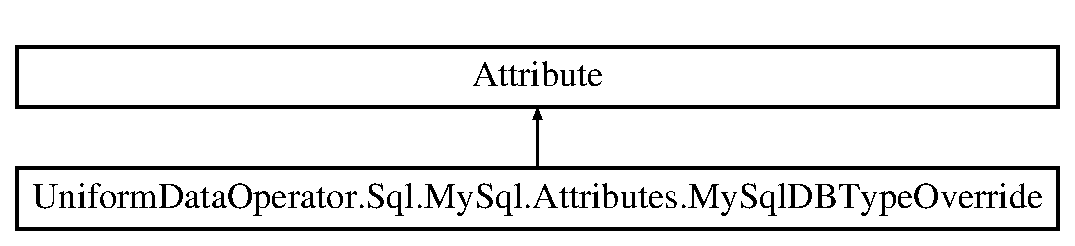
\includegraphics[height=2.000000cm]{dc/d3f/class_uniform_data_operator_1_1_sql_1_1_my_sql_1_1_attributes_1_1_my_sql_d_b_type_override}
\end{center}
\end{figure}
\subsection*{Public Member Functions}
\begin{DoxyCompactItemize}
\item 
\mbox{\hyperlink{class_uniform_data_operator_1_1_sql_1_1_my_sql_1_1_attributes_1_1_my_sql_d_b_type_override_aa560e25692613f1a6860f8991dc18a66}{My\+Sql\+D\+B\+Type\+Override}} (My\+Sql\+Db\+Type \mbox{\hyperlink{class_uniform_data_operator_1_1_sql_1_1_my_sql_1_1_attributes_1_1_my_sql_d_b_type_override_a6521991385a038d7f5878ab6bbcb5795}{type}})
\begin{DoxyCompactList}\small\item\em Overriding standard type\textquotesingle{}s definition of column and specifiy it for \mbox{\hyperlink{namespace_uniform_data_operator_1_1_sql_1_1_my_sql}{My\+Sql}} databases. \end{DoxyCompactList}\item 
\mbox{\hyperlink{class_uniform_data_operator_1_1_sql_1_1_my_sql_1_1_attributes_1_1_my_sql_d_b_type_override_acd28e7a908283c3cb18a0c83e701b85e}{My\+Sql\+D\+B\+Type\+Override}} (My\+Sql\+Db\+Type \mbox{\hyperlink{class_uniform_data_operator_1_1_sql_1_1_my_sql_1_1_attributes_1_1_my_sql_d_b_type_override_a6521991385a038d7f5878ab6bbcb5795}{type}}, string \mbox{\hyperlink{class_uniform_data_operator_1_1_sql_1_1_my_sql_1_1_attributes_1_1_my_sql_d_b_type_override_a708ba68a2b1ab31ed51c196bb3e4574f}{string\+Format}})
\begin{DoxyCompactList}\small\item\em Overriding standard type\textquotesingle{}s definition of column and specifiy it for \mbox{\hyperlink{namespace_uniform_data_operator_1_1_sql_1_1_my_sql}{My\+Sql}} databases. \end{DoxyCompactList}\end{DoxyCompactItemize}
\subsection*{Public Attributes}
\begin{DoxyCompactItemize}
\item 
My\+Sql\+Db\+Type \mbox{\hyperlink{class_uniform_data_operator_1_1_sql_1_1_my_sql_1_1_attributes_1_1_my_sql_d_b_type_override_a6521991385a038d7f5878ab6bbcb5795}{type}}
\begin{DoxyCompactList}\small\item\em Type relative to \mbox{\hyperlink{namespace_uniform_data_operator_1_1_sql_1_1_my_sql}{My\+Sql}} params. \end{DoxyCompactList}\item 
string \mbox{\hyperlink{class_uniform_data_operator_1_1_sql_1_1_my_sql_1_1_attributes_1_1_my_sql_d_b_type_override_a708ba68a2b1ab31ed51c196bb3e4574f}{string\+Format}}
\begin{DoxyCompactList}\small\item\em Type in string format that would be used during column declaration. Example\+: V\+A\+R\+C\+H\+A\+R(45), B\+L\+O\+B(4196) \end{DoxyCompactList}\end{DoxyCompactItemize}


\subsection{Detailed Description}
Attribute that can be defined to override standard D\+B\+Type defined in Column attribute, for columns that would created in \mbox{\hyperlink{namespace_uniform_data_operator_1_1_sql_1_1_my_sql}{My\+Sql}} tables. 



\subsection{Constructor \& Destructor Documentation}
\mbox{\Hypertarget{class_uniform_data_operator_1_1_sql_1_1_my_sql_1_1_attributes_1_1_my_sql_d_b_type_override_aa560e25692613f1a6860f8991dc18a66}\label{class_uniform_data_operator_1_1_sql_1_1_my_sql_1_1_attributes_1_1_my_sql_d_b_type_override_aa560e25692613f1a6860f8991dc18a66}} 
\index{Uniform\+Data\+Operator\+::\+Sql\+::\+My\+Sql\+::\+Attributes\+::\+My\+Sql\+D\+B\+Type\+Override@{Uniform\+Data\+Operator\+::\+Sql\+::\+My\+Sql\+::\+Attributes\+::\+My\+Sql\+D\+B\+Type\+Override}!My\+Sql\+D\+B\+Type\+Override@{My\+Sql\+D\+B\+Type\+Override}}
\index{My\+Sql\+D\+B\+Type\+Override@{My\+Sql\+D\+B\+Type\+Override}!Uniform\+Data\+Operator\+::\+Sql\+::\+My\+Sql\+::\+Attributes\+::\+My\+Sql\+D\+B\+Type\+Override@{Uniform\+Data\+Operator\+::\+Sql\+::\+My\+Sql\+::\+Attributes\+::\+My\+Sql\+D\+B\+Type\+Override}}
\subsubsection{\texorpdfstring{My\+Sql\+D\+B\+Type\+Override()}{MySqlDBTypeOverride()}\hspace{0.1cm}{\footnotesize\ttfamily [1/2]}}
{\footnotesize\ttfamily Uniform\+Data\+Operator.\+Sql.\+My\+Sql.\+Attributes.\+My\+Sql\+D\+B\+Type\+Override.\+My\+Sql\+D\+B\+Type\+Override (\begin{DoxyParamCaption}\item[{My\+Sql\+Db\+Type}]{type }\end{DoxyParamCaption})}



Overriding standard type\textquotesingle{}s definition of column and specifiy it for \mbox{\hyperlink{namespace_uniform_data_operator_1_1_sql_1_1_my_sql}{My\+Sql}} databases. 

Warning\+: unsafe method, cause just converts type to string to receive string\+Format value. Acceptable only for types that hasn\textquotesingle{}t params. T\+I\+N\+Y\+B\+L\+OB as example. 


\begin{DoxyParams}{Parameters}
{\em type} & Type relative to \mbox{\hyperlink{namespace_uniform_data_operator_1_1_sql_1_1_my_sql}{My\+Sql}} params.\\
\hline
\end{DoxyParams}
\mbox{\Hypertarget{class_uniform_data_operator_1_1_sql_1_1_my_sql_1_1_attributes_1_1_my_sql_d_b_type_override_acd28e7a908283c3cb18a0c83e701b85e}\label{class_uniform_data_operator_1_1_sql_1_1_my_sql_1_1_attributes_1_1_my_sql_d_b_type_override_acd28e7a908283c3cb18a0c83e701b85e}} 
\index{Uniform\+Data\+Operator\+::\+Sql\+::\+My\+Sql\+::\+Attributes\+::\+My\+Sql\+D\+B\+Type\+Override@{Uniform\+Data\+Operator\+::\+Sql\+::\+My\+Sql\+::\+Attributes\+::\+My\+Sql\+D\+B\+Type\+Override}!My\+Sql\+D\+B\+Type\+Override@{My\+Sql\+D\+B\+Type\+Override}}
\index{My\+Sql\+D\+B\+Type\+Override@{My\+Sql\+D\+B\+Type\+Override}!Uniform\+Data\+Operator\+::\+Sql\+::\+My\+Sql\+::\+Attributes\+::\+My\+Sql\+D\+B\+Type\+Override@{Uniform\+Data\+Operator\+::\+Sql\+::\+My\+Sql\+::\+Attributes\+::\+My\+Sql\+D\+B\+Type\+Override}}
\subsubsection{\texorpdfstring{My\+Sql\+D\+B\+Type\+Override()}{MySqlDBTypeOverride()}\hspace{0.1cm}{\footnotesize\ttfamily [2/2]}}
{\footnotesize\ttfamily Uniform\+Data\+Operator.\+Sql.\+My\+Sql.\+Attributes.\+My\+Sql\+D\+B\+Type\+Override.\+My\+Sql\+D\+B\+Type\+Override (\begin{DoxyParamCaption}\item[{My\+Sql\+Db\+Type}]{type,  }\item[{string}]{string\+Format }\end{DoxyParamCaption})}



Overriding standard type\textquotesingle{}s definition of column and specifiy it for \mbox{\hyperlink{namespace_uniform_data_operator_1_1_sql_1_1_my_sql}{My\+Sql}} databases. 


\begin{DoxyParams}{Parameters}
{\em type} & Type relative to \mbox{\hyperlink{namespace_uniform_data_operator_1_1_sql_1_1_my_sql}{My\+Sql}} params.\\
\hline
{\em string\+Format} & Type in string format that would be used during column declaration. Example\+: V\+A\+R\+C\+H\+A\+R(45), B\+L\+O\+B(4196)\\
\hline
\end{DoxyParams}


\subsection{Member Data Documentation}
\mbox{\Hypertarget{class_uniform_data_operator_1_1_sql_1_1_my_sql_1_1_attributes_1_1_my_sql_d_b_type_override_a708ba68a2b1ab31ed51c196bb3e4574f}\label{class_uniform_data_operator_1_1_sql_1_1_my_sql_1_1_attributes_1_1_my_sql_d_b_type_override_a708ba68a2b1ab31ed51c196bb3e4574f}} 
\index{Uniform\+Data\+Operator\+::\+Sql\+::\+My\+Sql\+::\+Attributes\+::\+My\+Sql\+D\+B\+Type\+Override@{Uniform\+Data\+Operator\+::\+Sql\+::\+My\+Sql\+::\+Attributes\+::\+My\+Sql\+D\+B\+Type\+Override}!string\+Format@{string\+Format}}
\index{string\+Format@{string\+Format}!Uniform\+Data\+Operator\+::\+Sql\+::\+My\+Sql\+::\+Attributes\+::\+My\+Sql\+D\+B\+Type\+Override@{Uniform\+Data\+Operator\+::\+Sql\+::\+My\+Sql\+::\+Attributes\+::\+My\+Sql\+D\+B\+Type\+Override}}
\subsubsection{\texorpdfstring{string\+Format}{stringFormat}}
{\footnotesize\ttfamily string Uniform\+Data\+Operator.\+Sql.\+My\+Sql.\+Attributes.\+My\+Sql\+D\+B\+Type\+Override.\+string\+Format}



Type in string format that would be used during column declaration. Example\+: V\+A\+R\+C\+H\+A\+R(45), B\+L\+O\+B(4196) 

\mbox{\Hypertarget{class_uniform_data_operator_1_1_sql_1_1_my_sql_1_1_attributes_1_1_my_sql_d_b_type_override_a6521991385a038d7f5878ab6bbcb5795}\label{class_uniform_data_operator_1_1_sql_1_1_my_sql_1_1_attributes_1_1_my_sql_d_b_type_override_a6521991385a038d7f5878ab6bbcb5795}} 
\index{Uniform\+Data\+Operator\+::\+Sql\+::\+My\+Sql\+::\+Attributes\+::\+My\+Sql\+D\+B\+Type\+Override@{Uniform\+Data\+Operator\+::\+Sql\+::\+My\+Sql\+::\+Attributes\+::\+My\+Sql\+D\+B\+Type\+Override}!type@{type}}
\index{type@{type}!Uniform\+Data\+Operator\+::\+Sql\+::\+My\+Sql\+::\+Attributes\+::\+My\+Sql\+D\+B\+Type\+Override@{Uniform\+Data\+Operator\+::\+Sql\+::\+My\+Sql\+::\+Attributes\+::\+My\+Sql\+D\+B\+Type\+Override}}
\subsubsection{\texorpdfstring{type}{type}}
{\footnotesize\ttfamily My\+Sql\+Db\+Type Uniform\+Data\+Operator.\+Sql.\+My\+Sql.\+Attributes.\+My\+Sql\+D\+B\+Type\+Override.\+type}



Type relative to \mbox{\hyperlink{namespace_uniform_data_operator_1_1_sql_1_1_my_sql}{My\+Sql}} params. 



The documentation for this class was generated from the following file\+:\begin{DoxyCompactItemize}
\item 
D\+:/\+Work/\+Git\+Hub/uniform-\/data-\/operator/\+S\+Q\+L/\+My\+S\+Q\+L/\+Attributes/My\+Sql\+D\+B\+Type\+Override.\+cs\end{DoxyCompactItemize}

\hypertarget{class_uniform_data_operator_1_1_sql_1_1_attributes_1_1_modifiers_1_1_set_query_ignore}{}\section{Uniform\+Data\+Operator.\+Sql.\+Attributes.\+Modifiers.\+Set\+Query\+Ignore Class Reference}
\label{class_uniform_data_operator_1_1_sql_1_1_attributes_1_1_modifiers_1_1_set_query_ignore}\index{Uniform\+Data\+Operator.\+Sql.\+Attributes.\+Modifiers.\+Set\+Query\+Ignore@{Uniform\+Data\+Operator.\+Sql.\+Attributes.\+Modifiers.\+Set\+Query\+Ignore}}


Can be defined to ignore of writing this value during set-\/like queries to server.  


Inheritance diagram for Uniform\+Data\+Operator.\+Sql.\+Attributes.\+Modifiers.\+Set\+Query\+Ignore\+:\begin{figure}[H]
\begin{center}
\leavevmode
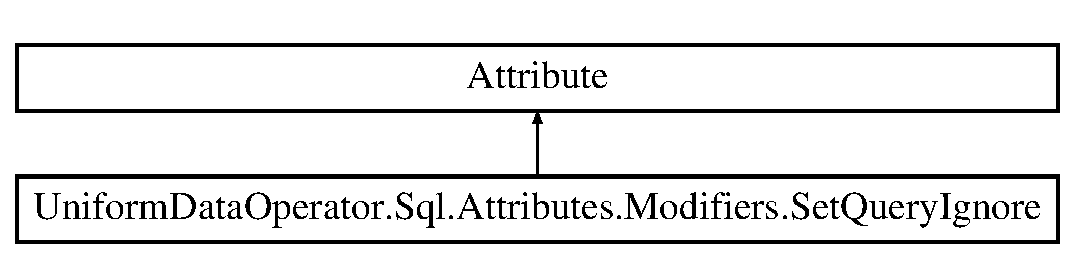
\includegraphics[height=2.000000cm]{db/ddc/class_uniform_data_operator_1_1_sql_1_1_attributes_1_1_modifiers_1_1_set_query_ignore}
\end{center}
\end{figure}


\subsection{Detailed Description}
Can be defined to ignore of writing this value during set-\/like queries to server. 



The documentation for this class was generated from the following file\+:\begin{DoxyCompactItemize}
\item 
D\+:/\+Work/\+Git\+Hub/uniform-\/data-\/operator/\+S\+Q\+L/\+Attributes/\+Modifiers/Set\+Query\+Ignore.\+cs\end{DoxyCompactItemize}

\hypertarget{class_uniform_data_operator_1_1_sql_1_1_sql_operator_handler}{}\section{Uniform\+Data\+Operator.\+Sql.\+Sql\+Operator\+Handler Class Reference}
\label{class_uniform_data_operator_1_1_sql_1_1_sql_operator_handler}\index{Uniform\+Data\+Operator.\+Sql.\+Sql\+Operator\+Handler@{Uniform\+Data\+Operator.\+Sql.\+Sql\+Operator\+Handler}}


Contains base catalog of uniform queries that strongly simplify managing of the data base.  


\subsection*{Static Public Member Functions}
\begin{DoxyCompactItemize}
\item 
static void \mbox{\hyperlink{class_uniform_data_operator_1_1_sql_1_1_sql_operator_handler_a898993886fbe98ece762f9f7f2af11fb}{Invoke\+S\+Q\+L\+Error\+Occured}} (object sender, string message)
\begin{DoxyCompactList}\small\item\em Invoke global error event informing about error occuring. \end{DoxyCompactList}\item 
static string \mbox{\hyperlink{class_uniform_data_operator_1_1_sql_1_1_sql_operator_handler_ab2de5b9d7f8e8e67b518cf39c7e6f7a5}{Collection\+To\+String}} (I\+Enumerable$<$ object $>$ collection)
\begin{DoxyCompactList}\small\item\em Conver collection view to string order. \end{DoxyCompactList}\item 
static string \mbox{\hyperlink{class_uniform_data_operator_1_1_sql_1_1_sql_operator_handler_a6973169901301adaecd52fab70df280e}{Concat\+Formated\+Collections}} (I\+Enumerable$<$ object $>$ headers, I\+Enumerable$<$ object $>$ values)
\begin{DoxyCompactList}\small\item\em Concat to collections in format\+: headers0 = \mbox{[}braket\mbox{]}values0\mbox{[}braket\mbox{]}, ..., headersN = \mbox{[}braket\mbox{]}valuesN\mbox{[}braket\mbox{]} \end{DoxyCompactList}\item 
static string \mbox{\hyperlink{class_uniform_data_operator_1_1_sql_1_1_sql_operator_handler_ac17e36b29fe5a17281927ab04dbeab26}{Concat\+Formated\+Collections}} (I\+Enumerable$<$ object $>$ headers, I\+Enumerable$<$ object $>$ values, char brackets\+Symbol)
\begin{DoxyCompactList}\small\item\em Concat to collections in format\+: headers0 = \mbox{[}braket\mbox{]}values0\mbox{[}braket\mbox{]}, ..., headersN = \mbox{[}braket\mbox{]}valuesN\mbox{[}braket\mbox{]} \end{DoxyCompactList}\item 
static bool \mbox{\hyperlink{class_uniform_data_operator_1_1_sql_1_1_sql_operator_handler_a97954b0bb1559fbe600c12aa5e2c53ef}{Database\+Data\+To\+Object}} (Db\+Data\+Reader reader, I\+Enumerable$<$ Member\+Info $>$ members, object obj, out string error)
\begin{DoxyCompactList}\small\item\em Trying to apply data base data to object by members map. \end{DoxyCompactList}\end{DoxyCompactItemize}
\subsection*{Properties}
\begin{DoxyCompactItemize}
\item 
static \mbox{\hyperlink{interface_uniform_data_operator_1_1_sql_1_1_i_sql_operator}{I\+Sql\+Operator}} \mbox{\hyperlink{class_uniform_data_operator_1_1_sql_1_1_sql_operator_handler_aa96eb9fd201700acbf53954599fec534}{Active}}\hspace{0.3cm}{\ttfamily  \mbox{[}get, set\mbox{]}}
\begin{DoxyCompactList}\small\item\em Contains las operator that asing itself to handler as active one. \end{DoxyCompactList}\end{DoxyCompactItemize}
\subsection*{Events}
\begin{DoxyCompactItemize}
\item 
static System.\+Action$<$ object, string $>$ \mbox{\hyperlink{class_uniform_data_operator_1_1_sql_1_1_sql_operator_handler_ab6cf915e80cf89b3e6eb14bf48a19185}{Sql\+Error\+Occured}}
\begin{DoxyCompactList}\small\item\em Event that can be called by operator to share errors during sql commands from async methods. \end{DoxyCompactList}\end{DoxyCompactItemize}


\subsection{Detailed Description}
Contains base catalog of uniform queries that strongly simplify managing of the data base. 



\subsection{Member Function Documentation}
\mbox{\Hypertarget{class_uniform_data_operator_1_1_sql_1_1_sql_operator_handler_ab2de5b9d7f8e8e67b518cf39c7e6f7a5}\label{class_uniform_data_operator_1_1_sql_1_1_sql_operator_handler_ab2de5b9d7f8e8e67b518cf39c7e6f7a5}} 
\index{Uniform\+Data\+Operator\+::\+Sql\+::\+Sql\+Operator\+Handler@{Uniform\+Data\+Operator\+::\+Sql\+::\+Sql\+Operator\+Handler}!Collection\+To\+String@{Collection\+To\+String}}
\index{Collection\+To\+String@{Collection\+To\+String}!Uniform\+Data\+Operator\+::\+Sql\+::\+Sql\+Operator\+Handler@{Uniform\+Data\+Operator\+::\+Sql\+::\+Sql\+Operator\+Handler}}
\subsubsection{\texorpdfstring{Collection\+To\+String()}{CollectionToString()}}
{\footnotesize\ttfamily static string Uniform\+Data\+Operator.\+Sql.\+Sql\+Operator\+Handler.\+Collection\+To\+String (\begin{DoxyParamCaption}\item[{I\+Enumerable$<$ object $>$}]{collection }\end{DoxyParamCaption})\hspace{0.3cm}{\ttfamily [static]}}



Conver collection view to string order. 

Elemets of collection must has overrided To\+String() methods. 


\begin{DoxyParams}{Parameters}
{\em collection} & Collection with strings,\\
\hline
\end{DoxyParams}
\begin{DoxyReturn}{Returns}
String in format\+: \char`\"{}i0, i1, ..., in\char`\"{}
\end{DoxyReturn}
\mbox{\Hypertarget{class_uniform_data_operator_1_1_sql_1_1_sql_operator_handler_a6973169901301adaecd52fab70df280e}\label{class_uniform_data_operator_1_1_sql_1_1_sql_operator_handler_a6973169901301adaecd52fab70df280e}} 
\index{Uniform\+Data\+Operator\+::\+Sql\+::\+Sql\+Operator\+Handler@{Uniform\+Data\+Operator\+::\+Sql\+::\+Sql\+Operator\+Handler}!Concat\+Formated\+Collections@{Concat\+Formated\+Collections}}
\index{Concat\+Formated\+Collections@{Concat\+Formated\+Collections}!Uniform\+Data\+Operator\+::\+Sql\+::\+Sql\+Operator\+Handler@{Uniform\+Data\+Operator\+::\+Sql\+::\+Sql\+Operator\+Handler}}
\subsubsection{\texorpdfstring{Concat\+Formated\+Collections()}{ConcatFormatedCollections()}\hspace{0.1cm}{\footnotesize\ttfamily [1/2]}}
{\footnotesize\ttfamily static string Uniform\+Data\+Operator.\+Sql.\+Sql\+Operator\+Handler.\+Concat\+Formated\+Collections (\begin{DoxyParamCaption}\item[{I\+Enumerable$<$ object $>$}]{headers,  }\item[{I\+Enumerable$<$ object $>$}]{values }\end{DoxyParamCaption})\hspace{0.3cm}{\ttfamily [static]}}



Concat to collections in format\+: headers0 = \mbox{[}braket\mbox{]}values0\mbox{[}braket\mbox{]}, ..., headersN = \mbox{[}braket\mbox{]}valuesN\mbox{[}braket\mbox{]} 

Elemets of collections must has overrided To\+String() methods. 


\begin{DoxyParams}{Parameters}
{\em headers} & Header of the value.\\
\hline
{\em values} & Value acording to header.\\
\hline
\end{DoxyParams}
\begin{DoxyReturn}{Returns}
String that contain collection suitable for S\+QL commands.
\end{DoxyReturn}
\mbox{\Hypertarget{class_uniform_data_operator_1_1_sql_1_1_sql_operator_handler_ac17e36b29fe5a17281927ab04dbeab26}\label{class_uniform_data_operator_1_1_sql_1_1_sql_operator_handler_ac17e36b29fe5a17281927ab04dbeab26}} 
\index{Uniform\+Data\+Operator\+::\+Sql\+::\+Sql\+Operator\+Handler@{Uniform\+Data\+Operator\+::\+Sql\+::\+Sql\+Operator\+Handler}!Concat\+Formated\+Collections@{Concat\+Formated\+Collections}}
\index{Concat\+Formated\+Collections@{Concat\+Formated\+Collections}!Uniform\+Data\+Operator\+::\+Sql\+::\+Sql\+Operator\+Handler@{Uniform\+Data\+Operator\+::\+Sql\+::\+Sql\+Operator\+Handler}}
\subsubsection{\texorpdfstring{Concat\+Formated\+Collections()}{ConcatFormatedCollections()}\hspace{0.1cm}{\footnotesize\ttfamily [2/2]}}
{\footnotesize\ttfamily static string Uniform\+Data\+Operator.\+Sql.\+Sql\+Operator\+Handler.\+Concat\+Formated\+Collections (\begin{DoxyParamCaption}\item[{I\+Enumerable$<$ object $>$}]{headers,  }\item[{I\+Enumerable$<$ object $>$}]{values,  }\item[{char}]{brackets\+Symbol }\end{DoxyParamCaption})\hspace{0.3cm}{\ttfamily [static]}}



Concat to collections in format\+: headers0 = \mbox{[}braket\mbox{]}values0\mbox{[}braket\mbox{]}, ..., headersN = \mbox{[}braket\mbox{]}valuesN\mbox{[}braket\mbox{]} 

Elemets of collections must has overrided To\+String() methods. 


\begin{DoxyParams}{Parameters}
{\em headers} & Header of the value.\\
\hline
{\em values} & Value acording to header.\\
\hline
{\em brackets\+Symbol} & Symbol that will has been using to clamp value.\\
\hline
\end{DoxyParams}
\begin{DoxyReturn}{Returns}
String that contain collection suitable for S\+QL commands.
\end{DoxyReturn}
\mbox{\Hypertarget{class_uniform_data_operator_1_1_sql_1_1_sql_operator_handler_a97954b0bb1559fbe600c12aa5e2c53ef}\label{class_uniform_data_operator_1_1_sql_1_1_sql_operator_handler_a97954b0bb1559fbe600c12aa5e2c53ef}} 
\index{Uniform\+Data\+Operator\+::\+Sql\+::\+Sql\+Operator\+Handler@{Uniform\+Data\+Operator\+::\+Sql\+::\+Sql\+Operator\+Handler}!Database\+Data\+To\+Object@{Database\+Data\+To\+Object}}
\index{Database\+Data\+To\+Object@{Database\+Data\+To\+Object}!Uniform\+Data\+Operator\+::\+Sql\+::\+Sql\+Operator\+Handler@{Uniform\+Data\+Operator\+::\+Sql\+::\+Sql\+Operator\+Handler}}
\subsubsection{\texorpdfstring{Database\+Data\+To\+Object()}{DatabaseDataToObject()}}
{\footnotesize\ttfamily static bool Uniform\+Data\+Operator.\+Sql.\+Sql\+Operator\+Handler.\+Database\+Data\+To\+Object (\begin{DoxyParamCaption}\item[{Db\+Data\+Reader}]{reader,  }\item[{I\+Enumerable$<$ Member\+Info $>$}]{members,  }\item[{object}]{obj,  }\item[{out string}]{error }\end{DoxyParamCaption})\hspace{0.3cm}{\ttfamily [static]}}



Trying to apply data base data to object by members map. 


\begin{DoxyParams}{Parameters}
{\em reader} & Data base data reader that contains data recived from server.\\
\hline
{\em members} & Map of members that would be lokking in reader.\\
\hline
{\em obj} & Target object that would contain output data.\\
\hline
{\em error} & Error occured during operation. Null if operation is success.\\
\hline
\end{DoxyParams}
\begin{DoxyReturn}{Returns}
Result of operation.
\end{DoxyReturn}
\mbox{\Hypertarget{class_uniform_data_operator_1_1_sql_1_1_sql_operator_handler_a898993886fbe98ece762f9f7f2af11fb}\label{class_uniform_data_operator_1_1_sql_1_1_sql_operator_handler_a898993886fbe98ece762f9f7f2af11fb}} 
\index{Uniform\+Data\+Operator\+::\+Sql\+::\+Sql\+Operator\+Handler@{Uniform\+Data\+Operator\+::\+Sql\+::\+Sql\+Operator\+Handler}!Invoke\+S\+Q\+L\+Error\+Occured@{Invoke\+S\+Q\+L\+Error\+Occured}}
\index{Invoke\+S\+Q\+L\+Error\+Occured@{Invoke\+S\+Q\+L\+Error\+Occured}!Uniform\+Data\+Operator\+::\+Sql\+::\+Sql\+Operator\+Handler@{Uniform\+Data\+Operator\+::\+Sql\+::\+Sql\+Operator\+Handler}}
\subsubsection{\texorpdfstring{Invoke\+S\+Q\+L\+Error\+Occured()}{InvokeSQLErrorOccured()}}
{\footnotesize\ttfamily static void Uniform\+Data\+Operator.\+Sql.\+Sql\+Operator\+Handler.\+Invoke\+S\+Q\+L\+Error\+Occured (\begin{DoxyParamCaption}\item[{object}]{sender,  }\item[{string}]{message }\end{DoxyParamCaption})\hspace{0.3cm}{\ttfamily [static]}}



Invoke global error event informing about error occuring. 



\subsection{Property Documentation}
\mbox{\Hypertarget{class_uniform_data_operator_1_1_sql_1_1_sql_operator_handler_aa96eb9fd201700acbf53954599fec534}\label{class_uniform_data_operator_1_1_sql_1_1_sql_operator_handler_aa96eb9fd201700acbf53954599fec534}} 
\index{Uniform\+Data\+Operator\+::\+Sql\+::\+Sql\+Operator\+Handler@{Uniform\+Data\+Operator\+::\+Sql\+::\+Sql\+Operator\+Handler}!Active@{Active}}
\index{Active@{Active}!Uniform\+Data\+Operator\+::\+Sql\+::\+Sql\+Operator\+Handler@{Uniform\+Data\+Operator\+::\+Sql\+::\+Sql\+Operator\+Handler}}
\subsubsection{\texorpdfstring{Active}{Active}}
{\footnotesize\ttfamily \mbox{\hyperlink{interface_uniform_data_operator_1_1_sql_1_1_i_sql_operator}{I\+Sql\+Operator}} Uniform\+Data\+Operator.\+Sql.\+Sql\+Operator\+Handler.\+Active\hspace{0.3cm}{\ttfamily [static]}, {\ttfamily [get]}, {\ttfamily [set]}}



Contains las operator that asing itself to handler as active one. 



\subsection{Event Documentation}
\mbox{\Hypertarget{class_uniform_data_operator_1_1_sql_1_1_sql_operator_handler_ab6cf915e80cf89b3e6eb14bf48a19185}\label{class_uniform_data_operator_1_1_sql_1_1_sql_operator_handler_ab6cf915e80cf89b3e6eb14bf48a19185}} 
\index{Uniform\+Data\+Operator\+::\+Sql\+::\+Sql\+Operator\+Handler@{Uniform\+Data\+Operator\+::\+Sql\+::\+Sql\+Operator\+Handler}!Sql\+Error\+Occured@{Sql\+Error\+Occured}}
\index{Sql\+Error\+Occured@{Sql\+Error\+Occured}!Uniform\+Data\+Operator\+::\+Sql\+::\+Sql\+Operator\+Handler@{Uniform\+Data\+Operator\+::\+Sql\+::\+Sql\+Operator\+Handler}}
\subsubsection{\texorpdfstring{Sql\+Error\+Occured}{SqlErrorOccured}}
{\footnotesize\ttfamily System.\+Action$<$object, string$>$ Uniform\+Data\+Operator.\+Sql.\+Sql\+Operator\+Handler.\+Sql\+Error\+Occured\hspace{0.3cm}{\ttfamily [static]}}



Event that can be called by operator to share errors during sql commands from async methods. 



The documentation for this class was generated from the following file\+:\begin{DoxyCompactItemize}
\item 
D\+:/\+Work/\+Git\+Hub/uniform-\/data-\/operator/\+S\+Q\+L/Sql\+Operator\+Handler.\+cs\end{DoxyCompactItemize}

\hypertarget{class_uniform_data_operator_1_1_sql_1_1_attributes_1_1_table}{}\section{Uniform\+Data\+Operator.\+Sql.\+Attributes.\+Table Class Reference}
\label{class_uniform_data_operator_1_1_sql_1_1_attributes_1_1_table}\index{Uniform\+Data\+Operator.\+Sql.\+Attributes.\+Table@{Uniform\+Data\+Operator.\+Sql.\+Attributes.\+Table}}


Attribute that would force to automatic generation of table on your S\+QL server suitable for declered members in class or structure.  


Inheritance diagram for Uniform\+Data\+Operator.\+Sql.\+Attributes.\+Table\+:\begin{figure}[H]
\begin{center}
\leavevmode
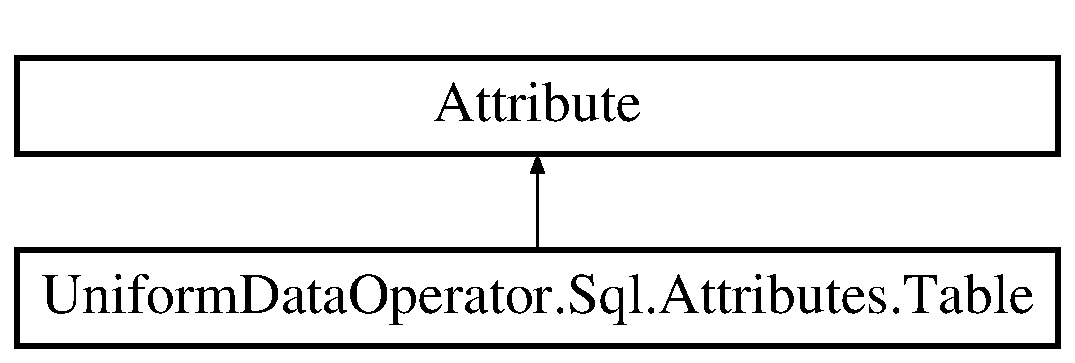
\includegraphics[height=2.000000cm]{dd/deb/class_uniform_data_operator_1_1_sql_1_1_attributes_1_1_table}
\end{center}
\end{figure}
\subsection*{Public Member Functions}
\begin{DoxyCompactItemize}
\item 
\mbox{\hyperlink{class_uniform_data_operator_1_1_sql_1_1_attributes_1_1_table_ad56af3278ca73f930b84b9dcbe777d5d}{Table}} (string \mbox{\hyperlink{class_uniform_data_operator_1_1_sql_1_1_attributes_1_1_table_a8390d02fa5d0b96ffd6e8f40cafefb7d}{schema}}, string \mbox{\hyperlink{class_uniform_data_operator_1_1_sql_1_1_attributes_1_1_table_ab413ed3bf0c1b110cf4b05cdea966de5}{table}})
\begin{DoxyCompactList}\small\item\em Configurate S\+QL table. \end{DoxyCompactList}\item 
\mbox{\hyperlink{class_uniform_data_operator_1_1_sql_1_1_attributes_1_1_table_a5c66b02de1ddfe8cd11ee4585ec77d82}{Table}} (string \mbox{\hyperlink{class_uniform_data_operator_1_1_sql_1_1_attributes_1_1_table_a8390d02fa5d0b96ffd6e8f40cafefb7d}{schema}}, string \mbox{\hyperlink{class_uniform_data_operator_1_1_sql_1_1_attributes_1_1_table_ab413ed3bf0c1b110cf4b05cdea966de5}{table}}, string \mbox{\hyperlink{class_uniform_data_operator_1_1_sql_1_1_attributes_1_1_table_afe0c2479401391900b1b16055a090e07}{engine}})
\begin{DoxyCompactList}\small\item\em Configurate S\+QL table. \end{DoxyCompactList}\end{DoxyCompactItemize}
\subsection*{Static Public Member Functions}
\begin{DoxyCompactItemize}
\item 
static string \mbox{\hyperlink{class_uniform_data_operator_1_1_sql_1_1_attributes_1_1_table_a4a18e92f3ee33003a7da468a9d5ab696}{Generate\+Create\+Table\+Command}} (Type source\+Type)
\begin{DoxyCompactList}\small\item\em Return command that would allow to create table by descriptor. \end{DoxyCompactList}\item 
static bool \mbox{\hyperlink{class_uniform_data_operator_1_1_sql_1_1_attributes_1_1_table_a0b905b5fd9ab2e381ce6cf81c3324a22}{Try\+Set\+Tables}} (bool disable\+S\+Q\+L\+Checks, out string error, params Type\mbox{[}$\,$\mbox{]} table\+Descriptors)
\begin{DoxyCompactList}\small\item\em Trying to set some tables to S\+QL server. Existed ones would be skiped. Not updating alter columns. \end{DoxyCompactList}\item 
static bool \mbox{\hyperlink{class_uniform_data_operator_1_1_sql_1_1_attributes_1_1_table_a80d799a2ba3419b489b9840f624880ff}{Try\+Set\+Table}} (bool disable\+S\+Q\+L\+Checks, Type table\+Descriptor, out string error)
\begin{DoxyCompactList}\small\item\em Trying to set table if required. Not updating alter columns. \end{DoxyCompactList}\item 
static List$<$ Member\+Info $>$ \mbox{\hyperlink{class_uniform_data_operator_1_1_sql_1_1_attributes_1_1_table_a7808fc23fc487fc878bd8d7869304ed1}{Find\+Members\+By\+Columns}} (I\+Enumerable$<$ Member\+Info $>$ members, params string\mbox{[}$\,$\mbox{]} column\+Titles)
\begin{DoxyCompactList}\small\item\em Looking for members that\textquotesingle{}s column\textquotesingle{}s titles included to array. \end{DoxyCompactList}\item 
static bool \mbox{\hyperlink{class_uniform_data_operator_1_1_sql_1_1_attributes_1_1_table_a8de48462eb10c4eddc660a2f19e96d0e}{Try\+To\+Get\+Table\+Attribute}} (Type table\+Type, out \mbox{\hyperlink{class_uniform_data_operator_1_1_sql_1_1_attributes_1_1_table}{Table}} table\+Descriptor, out string error)
\begin{DoxyCompactList}\small\item\em Looking for valid \mbox{\hyperlink{class_uniform_data_operator_1_1_sql_1_1_attributes_1_1_table}{Table}} attribute. Chack all overridings and return correct descriptor. \end{DoxyCompactList}\end{DoxyCompactItemize}
\subsection*{Public Attributes}
\begin{DoxyCompactItemize}
\item 
string \mbox{\hyperlink{class_uniform_data_operator_1_1_sql_1_1_attributes_1_1_table_a8390d02fa5d0b96ffd6e8f40cafefb7d}{schema}}
\begin{DoxyCompactList}\small\item\em Name of the holding schema. \end{DoxyCompactList}\item 
string \mbox{\hyperlink{class_uniform_data_operator_1_1_sql_1_1_attributes_1_1_table_ab413ed3bf0c1b110cf4b05cdea966de5}{table}}
\begin{DoxyCompactList}\small\item\em Name of the table. \end{DoxyCompactList}\item 
string \mbox{\hyperlink{class_uniform_data_operator_1_1_sql_1_1_attributes_1_1_table_afe0c2479401391900b1b16055a090e07}{engine}} = \char`\"{}Inno\+DB\char`\"{}
\begin{DoxyCompactList}\small\item\em Name of the database engine. \end{DoxyCompactList}\end{DoxyCompactItemize}


\subsection{Detailed Description}
Attribute that would force to automatic generation of table on your S\+QL server suitable for declered members in class or structure. 



\subsection{Constructor \& Destructor Documentation}
\mbox{\Hypertarget{class_uniform_data_operator_1_1_sql_1_1_attributes_1_1_table_ad56af3278ca73f930b84b9dcbe777d5d}\label{class_uniform_data_operator_1_1_sql_1_1_attributes_1_1_table_ad56af3278ca73f930b84b9dcbe777d5d}} 
\index{Uniform\+Data\+Operator\+::\+Sql\+::\+Attributes\+::\+Table@{Uniform\+Data\+Operator\+::\+Sql\+::\+Attributes\+::\+Table}!Table@{Table}}
\index{Table@{Table}!Uniform\+Data\+Operator\+::\+Sql\+::\+Attributes\+::\+Table@{Uniform\+Data\+Operator\+::\+Sql\+::\+Attributes\+::\+Table}}
\subsubsection{\texorpdfstring{Table()}{Table()}\hspace{0.1cm}{\footnotesize\ttfamily [1/2]}}
{\footnotesize\ttfamily Uniform\+Data\+Operator.\+Sql.\+Attributes.\+Table.\+Table (\begin{DoxyParamCaption}\item[{string}]{schema,  }\item[{string}]{table }\end{DoxyParamCaption})}



Configurate S\+QL table. 


\begin{DoxyParams}{Parameters}
{\em schema} & Name of foreign schema.\\
\hline
{\em table} & Name of foreign table.\\
\hline
\end{DoxyParams}
\mbox{\Hypertarget{class_uniform_data_operator_1_1_sql_1_1_attributes_1_1_table_a5c66b02de1ddfe8cd11ee4585ec77d82}\label{class_uniform_data_operator_1_1_sql_1_1_attributes_1_1_table_a5c66b02de1ddfe8cd11ee4585ec77d82}} 
\index{Uniform\+Data\+Operator\+::\+Sql\+::\+Attributes\+::\+Table@{Uniform\+Data\+Operator\+::\+Sql\+::\+Attributes\+::\+Table}!Table@{Table}}
\index{Table@{Table}!Uniform\+Data\+Operator\+::\+Sql\+::\+Attributes\+::\+Table@{Uniform\+Data\+Operator\+::\+Sql\+::\+Attributes\+::\+Table}}
\subsubsection{\texorpdfstring{Table()}{Table()}\hspace{0.1cm}{\footnotesize\ttfamily [2/2]}}
{\footnotesize\ttfamily Uniform\+Data\+Operator.\+Sql.\+Attributes.\+Table.\+Table (\begin{DoxyParamCaption}\item[{string}]{schema,  }\item[{string}]{table,  }\item[{string}]{engine }\end{DoxyParamCaption})}



Configurate S\+QL table. 


\begin{DoxyParams}{Parameters}
{\em schema} & Name of foreign schema.\\
\hline
{\em table} & Name of foreign table.\\
\hline
{\em engine} & Name of the database engine.\\
\hline
\end{DoxyParams}


\subsection{Member Function Documentation}
\mbox{\Hypertarget{class_uniform_data_operator_1_1_sql_1_1_attributes_1_1_table_a7808fc23fc487fc878bd8d7869304ed1}\label{class_uniform_data_operator_1_1_sql_1_1_attributes_1_1_table_a7808fc23fc487fc878bd8d7869304ed1}} 
\index{Uniform\+Data\+Operator\+::\+Sql\+::\+Attributes\+::\+Table@{Uniform\+Data\+Operator\+::\+Sql\+::\+Attributes\+::\+Table}!Find\+Members\+By\+Columns@{Find\+Members\+By\+Columns}}
\index{Find\+Members\+By\+Columns@{Find\+Members\+By\+Columns}!Uniform\+Data\+Operator\+::\+Sql\+::\+Attributes\+::\+Table@{Uniform\+Data\+Operator\+::\+Sql\+::\+Attributes\+::\+Table}}
\subsubsection{\texorpdfstring{Find\+Members\+By\+Columns()}{FindMembersByColumns()}}
{\footnotesize\ttfamily static List$<$Member\+Info$>$ Uniform\+Data\+Operator.\+Sql.\+Attributes.\+Table.\+Find\+Members\+By\+Columns (\begin{DoxyParamCaption}\item[{I\+Enumerable$<$ Member\+Info $>$}]{members,  }\item[{params string \mbox{[}$\,$\mbox{]}}]{column\+Titles }\end{DoxyParamCaption})\hspace{0.3cm}{\ttfamily [static]}}



Looking for members that\textquotesingle{}s column\textquotesingle{}s titles included to array. 


\begin{DoxyParams}{Parameters}
{\em members} & List of members that will be used for columns search.\\
\hline
{\em column\+Titles} & Array that contais column\textquotesingle{}s titles that would be looking among members.\\
\hline
\end{DoxyParams}
\begin{DoxyReturn}{Returns}
List with suitable members.
\end{DoxyReturn}
\mbox{\Hypertarget{class_uniform_data_operator_1_1_sql_1_1_attributes_1_1_table_a4a18e92f3ee33003a7da468a9d5ab696}\label{class_uniform_data_operator_1_1_sql_1_1_attributes_1_1_table_a4a18e92f3ee33003a7da468a9d5ab696}} 
\index{Uniform\+Data\+Operator\+::\+Sql\+::\+Attributes\+::\+Table@{Uniform\+Data\+Operator\+::\+Sql\+::\+Attributes\+::\+Table}!Generate\+Create\+Table\+Command@{Generate\+Create\+Table\+Command}}
\index{Generate\+Create\+Table\+Command@{Generate\+Create\+Table\+Command}!Uniform\+Data\+Operator\+::\+Sql\+::\+Attributes\+::\+Table@{Uniform\+Data\+Operator\+::\+Sql\+::\+Attributes\+::\+Table}}
\subsubsection{\texorpdfstring{Generate\+Create\+Table\+Command()}{GenerateCreateTableCommand()}}
{\footnotesize\ttfamily static string Uniform\+Data\+Operator.\+Sql.\+Attributes.\+Table.\+Generate\+Create\+Table\+Command (\begin{DoxyParamCaption}\item[{Type}]{source\+Type }\end{DoxyParamCaption})\hspace{0.3cm}{\ttfamily [static]}}



Return command that would allow to create table by descriptor. 


\begin{DoxyParams}{Parameters}
{\em source\+Type} & \\
\hline
\end{DoxyParams}
\begin{DoxyReturn}{Returns}

\end{DoxyReturn}
\mbox{\Hypertarget{class_uniform_data_operator_1_1_sql_1_1_attributes_1_1_table_a80d799a2ba3419b489b9840f624880ff}\label{class_uniform_data_operator_1_1_sql_1_1_attributes_1_1_table_a80d799a2ba3419b489b9840f624880ff}} 
\index{Uniform\+Data\+Operator\+::\+Sql\+::\+Attributes\+::\+Table@{Uniform\+Data\+Operator\+::\+Sql\+::\+Attributes\+::\+Table}!Try\+Set\+Table@{Try\+Set\+Table}}
\index{Try\+Set\+Table@{Try\+Set\+Table}!Uniform\+Data\+Operator\+::\+Sql\+::\+Attributes\+::\+Table@{Uniform\+Data\+Operator\+::\+Sql\+::\+Attributes\+::\+Table}}
\subsubsection{\texorpdfstring{Try\+Set\+Table()}{TrySetTable()}}
{\footnotesize\ttfamily static bool Uniform\+Data\+Operator.\+Sql.\+Attributes.\+Table.\+Try\+Set\+Table (\begin{DoxyParamCaption}\item[{bool}]{disable\+S\+Q\+L\+Checks,  }\item[{Type}]{table\+Descriptor,  }\item[{out string}]{error }\end{DoxyParamCaption})\hspace{0.3cm}{\ttfamily [static]}}



Trying to set table if required. Not updating alter columns. 


\begin{DoxyParams}{Parameters}
{\em disable\+S\+Q\+L\+Checks} & Disable check of data itegrity during command.\\
\hline
{\em table\+Descriptor} & Type that would be trying to recreate on your S\+QL server. Must has defined \mbox{\hyperlink{class_uniform_data_operator_1_1_sql_1_1_attributes_1_1_table}{Uniform\+Data\+Operator.\+Sql.\+Attributes.\+Table}} attribute.\\
\hline
{\em error} & Error faces during operation.\\
\hline
\end{DoxyParams}
\begin{DoxyReturn}{Returns}
Result of operation.
\end{DoxyReturn}
\mbox{\Hypertarget{class_uniform_data_operator_1_1_sql_1_1_attributes_1_1_table_a0b905b5fd9ab2e381ce6cf81c3324a22}\label{class_uniform_data_operator_1_1_sql_1_1_attributes_1_1_table_a0b905b5fd9ab2e381ce6cf81c3324a22}} 
\index{Uniform\+Data\+Operator\+::\+Sql\+::\+Attributes\+::\+Table@{Uniform\+Data\+Operator\+::\+Sql\+::\+Attributes\+::\+Table}!Try\+Set\+Tables@{Try\+Set\+Tables}}
\index{Try\+Set\+Tables@{Try\+Set\+Tables}!Uniform\+Data\+Operator\+::\+Sql\+::\+Attributes\+::\+Table@{Uniform\+Data\+Operator\+::\+Sql\+::\+Attributes\+::\+Table}}
\subsubsection{\texorpdfstring{Try\+Set\+Tables()}{TrySetTables()}}
{\footnotesize\ttfamily static bool Uniform\+Data\+Operator.\+Sql.\+Attributes.\+Table.\+Try\+Set\+Tables (\begin{DoxyParamCaption}\item[{bool}]{disable\+S\+Q\+L\+Checks,  }\item[{out string}]{error,  }\item[{params Type \mbox{[}$\,$\mbox{]}}]{table\+Descriptors }\end{DoxyParamCaption})\hspace{0.3cm}{\ttfamily [static]}}



Trying to set some tables to S\+QL server. Existed ones would be skiped. Not updating alter columns. 


\begin{DoxyParams}{Parameters}
{\em disable\+S\+Q\+L\+Checks} & Disable check of data itegrity during command.\\
\hline
{\em error} & Error cased during operation. Null if al passed without exceptions.\\
\hline
{\em table\+Descriptors} & Types with defined \char`\"{}\+Table\char`\"{} attribute.\\
\hline
\end{DoxyParams}
\begin{DoxyReturn}{Returns}
Result of operation.
\end{DoxyReturn}
\mbox{\Hypertarget{class_uniform_data_operator_1_1_sql_1_1_attributes_1_1_table_a8de48462eb10c4eddc660a2f19e96d0e}\label{class_uniform_data_operator_1_1_sql_1_1_attributes_1_1_table_a8de48462eb10c4eddc660a2f19e96d0e}} 
\index{Uniform\+Data\+Operator\+::\+Sql\+::\+Attributes\+::\+Table@{Uniform\+Data\+Operator\+::\+Sql\+::\+Attributes\+::\+Table}!Try\+To\+Get\+Table\+Attribute@{Try\+To\+Get\+Table\+Attribute}}
\index{Try\+To\+Get\+Table\+Attribute@{Try\+To\+Get\+Table\+Attribute}!Uniform\+Data\+Operator\+::\+Sql\+::\+Attributes\+::\+Table@{Uniform\+Data\+Operator\+::\+Sql\+::\+Attributes\+::\+Table}}
\subsubsection{\texorpdfstring{Try\+To\+Get\+Table\+Attribute()}{TryToGetTableAttribute()}}
{\footnotesize\ttfamily static bool Uniform\+Data\+Operator.\+Sql.\+Attributes.\+Table.\+Try\+To\+Get\+Table\+Attribute (\begin{DoxyParamCaption}\item[{Type}]{table\+Type,  }\item[{out \mbox{\hyperlink{class_uniform_data_operator_1_1_sql_1_1_attributes_1_1_table}{Table}}}]{table\+Descriptor,  }\item[{out string}]{error }\end{DoxyParamCaption})\hspace{0.3cm}{\ttfamily [static]}}



Looking for valid \mbox{\hyperlink{class_uniform_data_operator_1_1_sql_1_1_attributes_1_1_table}{Table}} attribute. Chack all overridings and return correct descriptor. 


\begin{DoxyParams}{Parameters}
{\em table\+Type} & Type that contains defined \mbox{\hyperlink{class_uniform_data_operator_1_1_sql_1_1_attributes_1_1_table}{Table}} attribute.\\
\hline
{\em table\+Descriptor} & Output table descriptor.\\
\hline
{\em error} & Error message in cvase if occured. Null in other case.\\
\hline
\end{DoxyParams}
\begin{DoxyReturn}{Returns}

\end{DoxyReturn}


\subsection{Member Data Documentation}
\mbox{\Hypertarget{class_uniform_data_operator_1_1_sql_1_1_attributes_1_1_table_afe0c2479401391900b1b16055a090e07}\label{class_uniform_data_operator_1_1_sql_1_1_attributes_1_1_table_afe0c2479401391900b1b16055a090e07}} 
\index{Uniform\+Data\+Operator\+::\+Sql\+::\+Attributes\+::\+Table@{Uniform\+Data\+Operator\+::\+Sql\+::\+Attributes\+::\+Table}!engine@{engine}}
\index{engine@{engine}!Uniform\+Data\+Operator\+::\+Sql\+::\+Attributes\+::\+Table@{Uniform\+Data\+Operator\+::\+Sql\+::\+Attributes\+::\+Table}}
\subsubsection{\texorpdfstring{engine}{engine}}
{\footnotesize\ttfamily string Uniform\+Data\+Operator.\+Sql.\+Attributes.\+Table.\+engine = \char`\"{}Inno\+DB\char`\"{}}



Name of the database engine. 

\mbox{\Hypertarget{class_uniform_data_operator_1_1_sql_1_1_attributes_1_1_table_a8390d02fa5d0b96ffd6e8f40cafefb7d}\label{class_uniform_data_operator_1_1_sql_1_1_attributes_1_1_table_a8390d02fa5d0b96ffd6e8f40cafefb7d}} 
\index{Uniform\+Data\+Operator\+::\+Sql\+::\+Attributes\+::\+Table@{Uniform\+Data\+Operator\+::\+Sql\+::\+Attributes\+::\+Table}!schema@{schema}}
\index{schema@{schema}!Uniform\+Data\+Operator\+::\+Sql\+::\+Attributes\+::\+Table@{Uniform\+Data\+Operator\+::\+Sql\+::\+Attributes\+::\+Table}}
\subsubsection{\texorpdfstring{schema}{schema}}
{\footnotesize\ttfamily string Uniform\+Data\+Operator.\+Sql.\+Attributes.\+Table.\+schema}



Name of the holding schema. 

\mbox{\Hypertarget{class_uniform_data_operator_1_1_sql_1_1_attributes_1_1_table_ab413ed3bf0c1b110cf4b05cdea966de5}\label{class_uniform_data_operator_1_1_sql_1_1_attributes_1_1_table_ab413ed3bf0c1b110cf4b05cdea966de5}} 
\index{Uniform\+Data\+Operator\+::\+Sql\+::\+Attributes\+::\+Table@{Uniform\+Data\+Operator\+::\+Sql\+::\+Attributes\+::\+Table}!table@{table}}
\index{table@{table}!Uniform\+Data\+Operator\+::\+Sql\+::\+Attributes\+::\+Table@{Uniform\+Data\+Operator\+::\+Sql\+::\+Attributes\+::\+Table}}
\subsubsection{\texorpdfstring{table}{table}}
{\footnotesize\ttfamily string Uniform\+Data\+Operator.\+Sql.\+Attributes.\+Table.\+table}



Name of the table. 



The documentation for this class was generated from the following file\+:\begin{DoxyCompactItemize}
\item 
D\+:/\+Work/\+Git\+Hub/uniform-\/data-\/operator/\+S\+Q\+L/\+Attributes/Table.\+cs\end{DoxyCompactItemize}

\hypertarget{class_base_tests_1_1_types_1_1_table2_type}{}\section{Base\+Tests.\+Types.\+Table2\+Type Class Reference}
\label{class_base_tests_1_1_types_1_1_table2_type}\index{Base\+Tests.\+Types.\+Table2\+Type@{Base\+Tests.\+Types.\+Table2\+Type}}
\subsection*{Public Attributes}
\begin{DoxyCompactItemize}
\item 
\mbox{\Hypertarget{class_base_tests_1_1_types_1_1_table2_type_a2de891713a0dc1d7e774bb0bdad1ef3c}\label{class_base_tests_1_1_types_1_1_table2_type_a2de891713a0dc1d7e774bb0bdad1ef3c}} 
int {\bfseries int\+FK}
\item 
\mbox{\Hypertarget{class_base_tests_1_1_types_1_1_table2_type_adb1d8b5e52be3103e77e032916aa6d88}\label{class_base_tests_1_1_types_1_1_table2_type_adb1d8b5e52be3103e77e032916aa6d88}} 
string {\bfseries string\+Var} = \char`\"{}test\+String\char`\"{}
\end{DoxyCompactItemize}


The documentation for this class was generated from the following file\+:\begin{DoxyCompactItemize}
\item 
D\+:/\+Work/\+Git\+Hub/uniform-\/data-\/operator/\+Tests/\+Base\+Tests/\+Types/Table2\+Type.\+cs\end{DoxyCompactItemize}

\hypertarget{class_base_tests_1_1_types_1_1_table3_type}{}\section{Base\+Tests.\+Types.\+Table3\+Type Class Reference}
\label{class_base_tests_1_1_types_1_1_table3_type}\index{Base\+Tests.\+Types.\+Table3\+Type@{Base\+Tests.\+Types.\+Table3\+Type}}
\subsection*{Public Attributes}
\begin{DoxyCompactItemize}
\item 
\mbox{\Hypertarget{class_base_tests_1_1_types_1_1_table3_type_adbab457a69b0bbbc8bc2807e19a2793d}\label{class_base_tests_1_1_types_1_1_table3_type_adbab457a69b0bbbc8bc2807e19a2793d}} 
int {\bfseries int\+FK}
\item 
\mbox{\Hypertarget{class_base_tests_1_1_types_1_1_table3_type_ab1c6286c3999dc909fcf2dd9b9836da1}\label{class_base_tests_1_1_types_1_1_table3_type_ab1c6286c3999dc909fcf2dd9b9836da1}} 
int {\bfseries int\+P\+K\+AI}
\item 
\mbox{\Hypertarget{class_base_tests_1_1_types_1_1_table3_type_abd686cdb0d1bc99ed5281c5a6128d39e}\label{class_base_tests_1_1_types_1_1_table3_type_abd686cdb0d1bc99ed5281c5a6128d39e}} 
string {\bfseries string\+Var} = \char`\"{}test\+String\char`\"{}
\end{DoxyCompactItemize}


The documentation for this class was generated from the following file\+:\begin{DoxyCompactItemize}
\item 
D\+:/\+Work/\+Git\+Hub/uniform-\/data-\/operator/\+Tests/\+Base\+Tests/\+Types/Table3\+Type.\+cs\end{DoxyCompactItemize}

\hypertarget{class_base_tests_1_1_types_1_1_table4_type}{}\section{Base\+Tests.\+Types.\+Table4\+Type Class Reference}
\label{class_base_tests_1_1_types_1_1_table4_type}\index{Base\+Tests.\+Types.\+Table4\+Type@{Base\+Tests.\+Types.\+Table4\+Type}}
\subsection*{Public Attributes}
\begin{DoxyCompactItemize}
\item 
\mbox{\Hypertarget{class_base_tests_1_1_types_1_1_table4_type_abd9dec41fe331ba2b57dda96f660f603}\label{class_base_tests_1_1_types_1_1_table4_type_abd9dec41fe331ba2b57dda96f660f603}} 
int {\bfseries int\+P\+K\+AI}
\item 
\mbox{\Hypertarget{class_base_tests_1_1_types_1_1_table4_type_a074de14ad3b69717e4eca6a7e714e1c5}\label{class_base_tests_1_1_types_1_1_table4_type_a074de14ad3b69717e4eca6a7e714e1c5}} 
string {\bfseries string\+Var} = \char`\"{}test\+String\char`\"{}
\end{DoxyCompactItemize}


The documentation for this class was generated from the following file\+:\begin{DoxyCompactItemize}
\item 
D\+:/\+Work/\+Git\+Hub/uniform-\/data-\/operator/\+Tests/\+Base\+Tests/\+Types/Table4\+Type.\+cs\end{DoxyCompactItemize}

\hypertarget{class_base_tests_1_1_types_1_1_table5_type}{}\section{Base\+Tests.\+Types.\+Table5\+Type Class Reference}
\label{class_base_tests_1_1_types_1_1_table5_type}\index{Base\+Tests.\+Types.\+Table5\+Type@{Base\+Tests.\+Types.\+Table5\+Type}}
\subsection*{Public Attributes}
\begin{DoxyCompactItemize}
\item 
\mbox{\Hypertarget{class_base_tests_1_1_types_1_1_table5_type_ae14f965f57c11a3a98b3b0533ef26f13}\label{class_base_tests_1_1_types_1_1_table5_type_ae14f965f57c11a3a98b3b0533ef26f13}} 
int {\bfseries int\+P\+K\+AI}
\item 
\mbox{\Hypertarget{class_base_tests_1_1_types_1_1_table5_type_ae30aa67ba478910dd4e0d7872e898f83}\label{class_base_tests_1_1_types_1_1_table5_type_ae30aa67ba478910dd4e0d7872e898f83}} 
string {\bfseries string\+Var} = \char`\"{}test\+String\char`\"{}
\end{DoxyCompactItemize}


The documentation for this class was generated from the following file\+:\begin{DoxyCompactItemize}
\item 
D\+:/\+Work/\+Git\+Hub/uniform-\/data-\/operator/\+Tests/\+Base\+Tests/\+Types/Table5\+Type.\+cs\end{DoxyCompactItemize}

\hypertarget{class_my_s_q_l_tests_1_1_tables}{}\section{My\+S\+Q\+L\+Tests.\+Tables Class Reference}
\label{class_my_s_q_l_tests_1_1_tables}\index{My\+S\+Q\+L\+Tests.\+Tables@{My\+S\+Q\+L\+Tests.\+Tables}}
\subsection*{Public Member Functions}
\begin{DoxyCompactItemize}
\item 
void \mbox{\hyperlink{class_my_s_q_l_tests_1_1_tables_ae9a63c27e5b8bae040555a7d633de210}{Connection}} ()
\begin{DoxyCompactList}\small\item\em Checking connection to database server. \end{DoxyCompactList}\item 
void \mbox{\hyperlink{class_my_s_q_l_tests_1_1_tables_a8b0f4f83fdeedb1cba72d520644b3bd9}{Generate}} ()
\begin{DoxyCompactList}\small\item\em Generating the test\textquotesingle{}s tables. \end{DoxyCompactList}\end{DoxyCompactItemize}
\subsection*{Static Public Member Functions}
\begin{DoxyCompactItemize}
\item 
static void \mbox{\hyperlink{class_my_s_q_l_tests_1_1_tables_a2bf30026249403d4a1764d4bc88af649}{Set\+Default}} ()
\begin{DoxyCompactList}\small\item\em Setting default S\+QL operator. \end{DoxyCompactList}\end{DoxyCompactItemize}


\subsection{Member Function Documentation}
\mbox{\Hypertarget{class_my_s_q_l_tests_1_1_tables_ae9a63c27e5b8bae040555a7d633de210}\label{class_my_s_q_l_tests_1_1_tables_ae9a63c27e5b8bae040555a7d633de210}} 
\index{My\+S\+Q\+L\+Tests\+::\+Tables@{My\+S\+Q\+L\+Tests\+::\+Tables}!Connection@{Connection}}
\index{Connection@{Connection}!My\+S\+Q\+L\+Tests\+::\+Tables@{My\+S\+Q\+L\+Tests\+::\+Tables}}
\subsubsection{\texorpdfstring{Connection()}{Connection()}}
{\footnotesize\ttfamily void My\+S\+Q\+L\+Tests.\+Tables.\+Connection (\begin{DoxyParamCaption}{ }\end{DoxyParamCaption})}



Checking connection to database server. 

\mbox{\Hypertarget{class_my_s_q_l_tests_1_1_tables_a8b0f4f83fdeedb1cba72d520644b3bd9}\label{class_my_s_q_l_tests_1_1_tables_a8b0f4f83fdeedb1cba72d520644b3bd9}} 
\index{My\+S\+Q\+L\+Tests\+::\+Tables@{My\+S\+Q\+L\+Tests\+::\+Tables}!Generate@{Generate}}
\index{Generate@{Generate}!My\+S\+Q\+L\+Tests\+::\+Tables@{My\+S\+Q\+L\+Tests\+::\+Tables}}
\subsubsection{\texorpdfstring{Generate()}{Generate()}}
{\footnotesize\ttfamily void My\+S\+Q\+L\+Tests.\+Tables.\+Generate (\begin{DoxyParamCaption}{ }\end{DoxyParamCaption})}



Generating the test\textquotesingle{}s tables. 

\mbox{\Hypertarget{class_my_s_q_l_tests_1_1_tables_a2bf30026249403d4a1764d4bc88af649}\label{class_my_s_q_l_tests_1_1_tables_a2bf30026249403d4a1764d4bc88af649}} 
\index{My\+S\+Q\+L\+Tests\+::\+Tables@{My\+S\+Q\+L\+Tests\+::\+Tables}!Set\+Default@{Set\+Default}}
\index{Set\+Default@{Set\+Default}!My\+S\+Q\+L\+Tests\+::\+Tables@{My\+S\+Q\+L\+Tests\+::\+Tables}}
\subsubsection{\texorpdfstring{Set\+Default()}{SetDefault()}}
{\footnotesize\ttfamily static void My\+S\+Q\+L\+Tests.\+Tables.\+Set\+Default (\begin{DoxyParamCaption}{ }\end{DoxyParamCaption})\hspace{0.3cm}{\ttfamily [static]}}



Setting default S\+QL operator. 



The documentation for this class was generated from the following file\+:\begin{DoxyCompactItemize}
\item 
D\+:/\+Work/\+Git\+Hub/uniform-\/data-\/operator/\+Tests/\+My\+S\+Q\+L\+Tests/Tables.\+cs\end{DoxyCompactItemize}

\hypertarget{class_base_tests_1_1_types_1_1_table_type}{}\section{Base\+Tests.\+Types.\+Table\+Type Class Reference}
\label{class_base_tests_1_1_types_1_1_table_type}\index{Base\+Tests.\+Types.\+Table\+Type@{Base\+Tests.\+Types.\+Table\+Type}}
\subsection*{Public Attributes}
\begin{DoxyCompactItemize}
\item 
\mbox{\Hypertarget{class_base_tests_1_1_types_1_1_table_type_abb14850439cf72cba85bad7b4c54f32f}\label{class_base_tests_1_1_types_1_1_table_type_abb14850439cf72cba85bad7b4c54f32f}} 
int {\bfseries pk}
\item 
\mbox{\Hypertarget{class_base_tests_1_1_types_1_1_table_type_ac96fc61cbc59ca606a19fbb72ec42ff0}\label{class_base_tests_1_1_types_1_1_table_type_ac96fc61cbc59ca606a19fbb72ec42ff0}} 
int {\bfseries int\+Var}
\item 
\mbox{\Hypertarget{class_base_tests_1_1_types_1_1_table_type_a6078c0d18572937a59ff4b4dc0a94522}\label{class_base_tests_1_1_types_1_1_table_type_a6078c0d18572937a59ff4b4dc0a94522}} 
int {\bfseries \+\_\+int\+Prop} = 123456
\item 
\mbox{\Hypertarget{class_base_tests_1_1_types_1_1_table_type_a5584287994bbf69958866d3ad23feeff}\label{class_base_tests_1_1_types_1_1_table_type_a5584287994bbf69958866d3ad23feeff}} 
uint {\bfseries uint\+Var} = 4
\item 
\mbox{\Hypertarget{class_base_tests_1_1_types_1_1_table_type_a425a914b6ee5c1dff7fa2f47d8c57fc2}\label{class_base_tests_1_1_types_1_1_table_type_a425a914b6ee5c1dff7fa2f47d8c57fc2}} 
int {\bfseries fk} = 4
\item 
\mbox{\Hypertarget{class_base_tests_1_1_types_1_1_table_type_abb4e5f2a420c546fc70a4aa725151118}\label{class_base_tests_1_1_types_1_1_table_type_abb4e5f2a420c546fc70a4aa725151118}} 
\mbox{\hyperlink{class_base_tests_1_1_types_1_1_blob_type}{Blob\+Type}} {\bfseries blob}
\end{DoxyCompactItemize}
\subsection*{Properties}
\begin{DoxyCompactItemize}
\item 
\mbox{\Hypertarget{class_base_tests_1_1_types_1_1_table_type_a08cf8ecd229624514fd695b2259e689d}\label{class_base_tests_1_1_types_1_1_table_type_a08cf8ecd229624514fd695b2259e689d}} 
int {\bfseries Int\+Prop}\hspace{0.3cm}{\ttfamily  \mbox{[}get, set\mbox{]}}
\item 
\mbox{\Hypertarget{class_base_tests_1_1_types_1_1_table_type_aa2bea278a987cb00b79198501cdd233b}\label{class_base_tests_1_1_types_1_1_table_type_aa2bea278a987cb00b79198501cdd233b}} 
byte \mbox{[}$\,$\mbox{]} {\bfseries Blob\+Prop}\hspace{0.3cm}{\ttfamily  \mbox{[}get, set\mbox{]}}
\end{DoxyCompactItemize}


The documentation for this class was generated from the following file\+:\begin{DoxyCompactItemize}
\item 
D\+:/\+Work/\+Git\+Hub/uniform-\/data-\/operator/\+Tests/\+Base\+Tests/\+Types/Table\+Type.\+cs\end{DoxyCompactItemize}

%--- End generated contents ---

% Index
\backmatter
\newpage
\phantomsection
\clearemptydoublepage
\addcontentsline{toc}{chapter}{Index}
\printindex

\end{document}
